%% LyX 2.3.6.1 created this file.  For more info, see http://www.lyx.org/.
%% Do not edit unless you really know what you are doing.
\documentclass[twoside,english]{article}
\usepackage[T1]{fontenc}
\usepackage[latin9]{inputenc}
\usepackage{geometry}
\geometry{verbose,tmargin=2cm,bmargin=2cm,lmargin=2cm,rmargin=2cm}
\usepackage{color}
\usepackage{amsmath}
\usepackage{amssymb}

\makeatletter
%%%%%%%%%%%%%%%%%%%%%%%%%%%%%% User specified LaTeX commands.
\usepackage{helvet}
\renewcommand{\familydefault}{\sfdefault}
\usepackage[T1]{fontenc}
\usepackage[latin9]{inputenc}
\usepackage{geometry}
\geometry{verbose,tmargin=1.8cm,bmargin=4cm,lmargin=1.5cm,rmargin=2cm}
\usepackage{enumitem}
\usepackage{amstext}
\usepackage{amsthm}
\usepackage{amssymb}
\usepackage{setspace}
\usepackage{graphicx}
\doublespacing


\usepackage{enumitem}
\setenumerate[1]{label=\textbf{\arabic*}}
\setenumerate[2]{label=\textbf{(\alph*)}}
\setenumerate[3]{label=\textbf{(\roman*)}}
\setlist[enumerate]{align=right}

\setcounter{page}{2}

%for upright integrals
\usepackage[integrals]{wasysym}

%to be used in conjunction with fancyfoot for last page
\usepackage{zref-totpages}

%fancyhrd settings
\usepackage{fancyhdr}
\pagestyle{fancy}
\fancyhf{}

\fancypagestyle{laststyle}
{
   \fancyhf{}
   \chead{\thepage}
   \fancyfoot[L]{\copyright NJC }
   \fancyfoot[R]{\textbf{END}} %Put \thispagestyle{laststyle} in the last page
}

%%centering page number
\chead{\thepage}

\renewcommand{\headrulewidth}{0pt}
\renewcommand{\footrulewidth}{0pt}

%%footer settings, different footer for ODD and EVEN pages, also for the LASTPAGE
\fancyfoot[LO]{Generated with Python Script by BRW\hfill \textbf{[Turn Over}}
\fancyfoot[LE]{Generated with Python Script by BRW }

%%shameless self-plug BRW

\makeatother

\usepackage{babel}
\begin{document}

\begin{enumerate}\item \textbf{{[}DHS/PRELIM/9597/2019/P1/Q1{]} }

The file \texttt{IOI19.TXT} stores the scoreboard of the 31st International
Olympiad in Informatics (IOI) held in Baku, Azerbaijan from 4 to 11
August 2019. The first line contains the header with contestant's
rank, name, team (country), and overall score. The remaining lines
contain the corresponding data. IOI 2019 eventually awarded 28 Gold,
54 Silver and 81 Bronze medals. A country typically sends up to 4
contestants to participate in IOI. 

\subsection*{Task 1.1 }

Determine the top 3 teams in the competition and display their country
names as well as the number of Gold, Silver and Bronze medals attained.
Teams which are tied will be ordered by their country names in alphabetical
order and will share the same rank. 

Sample output: 

\texttt{Top 3 teams: }

\texttt{1 ABC 4G }

\texttt{2 DEF 3G1S }

\texttt{2 GHI 3G1S }

\texttt{4 JKL 2G1S1B }

\texttt{4 MNO 2G1S1B }

\subsection*{Evidence 1 }

Program code. \hfill{}{[}9{]}

\subsection*{Evidence 2 }

Screenshot. \hfill{} {[}1{]}

\subsection*{Task 1.2 }

Write program code to prompt a user to enter a team name and display
the results of its participants. Participants who did not receive
a medal will be denoted with \texttt{P}. The program will terminate
when a user enters the text string \texttt{'ZZZ'} (without the quotes). 

Sample interaction: 

\texttt{Enter team: SGP }

\texttt{Eu-Shaun Leong G }

\texttt{Lee Jeffrey Chun Hean S }

\texttt{Benson Zhan Li Lin B }

\texttt{Daniel Zhenghao Choo P }

\texttt{Enter team: ZZZ }

\texttt{Bye }

\subsection*{Evidence 3}

Program code. \hfill{} {[}4{]}

\subsection*{Evidence 4 }

Screenshot. \hfill{}{[}1{]}

 \newpage 

\item \textbf{{[}DHS/PRELIM/9597/2019/P1/Q2{]} }

Dubbed first of its kind globally, the Singapore Quick Response Code
(SGQR) is an infrastructure-light technology that will help to simplify
QR e-payments in Singapore for both consumers and merchants. 

The SGQR is based on the QR Code Specification for Payment System
- Merchant-Presented Mode standard issued by EMVCo, which has the
benefits of international interoperability, multi-tenancy of QR schemes
and non-sensitive data presented for payments. 

According to the specification, the parsed SGQR text string contains
data items, with each data item adhering to the following structure:
id, length, value. Two such data items are highlighted in bold in
the following diagram: 
\begin{center}
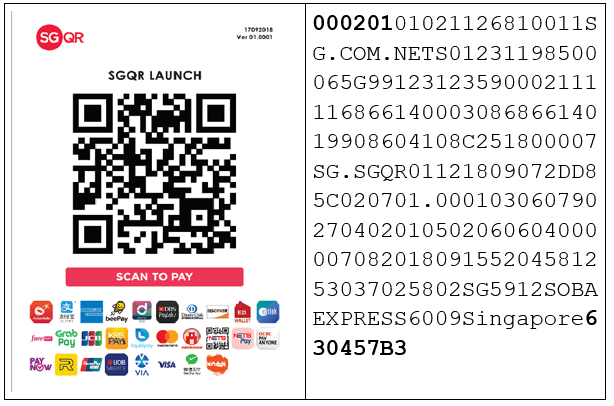
\includegraphics[width=0.5\paperwidth]{C:/Users/Admin/Desktop/Github/question_bank/LyX/static/img/9597-DHS-2019-P1-Q2}
\par\end{center}

Thus for the first data item \texttt{\textbf{000201}}, \texttt{00}
is the id, \texttt{02} is the length, and \texttt{01} is the value. 

And for the last data item \texttt{\textbf{630457B3}}, \texttt{63}
is the id, \texttt{04} is the length, and \texttt{57B3} is the value. 

The value \texttt{57B3} is also a hexdecimal number to verify the
integrity of the SGQR data. 

\subsection*{Task 2.1 }

Write program code to extract the last data item of the SGQR stored
in \texttt{SGQR.TXT}. For the example above, it will be the data item
with id 63 and length 4 i.e. 630457B3. 

\subsection*{Evidence 5 }

Program code. \hfill{} {[}3{]}

\subsection*{Evidence 6 }

Screenshot. \hfill{} {[}1{]}

\subsection*{Task 2.2 }

Write a \texttt{hex2oct} function which takes in a hexadecimal number
string and returns its equivalent octal number string. For example
\texttt{hex2oct('A')} returns \texttt{'12'}. You may not use Python's
built in \texttt{int(num, 8)}, \texttt{int(num, 16)}, \texttt{bin()},
\texttt{oct()} or \texttt{hex()} functions. Use the hexadecimal number
string \texttt{'4F63A'} to to test your program code. 

Hint: One hexadecimal digit can be expressed as four binary digits
and one octal digit can be expressed as three binary digits. 

\subsection*{Evidence 7 }

Program code. \hfill{}{[}5{]}

\subsection*{Evidence 8 }

Screenshot. \hfill{}{[}1{]}

\subsection*{Task 2.3 }

Write program code to perform input validation for a hexadecimal number
string. Test your program with suitable test data. 

\subsection*{Evidence 9 }

Program code. \hfill{}{[}3{]}

\subsection*{Evidence 10 }

Screenshots. \hfill{}{[}2{]}

 \newpage 

\item \textbf{{[}DHS/PRELIM/9597/2019/P1/Q3{]} }

From 2021 onwards, the Primary School Leaving Exam (PSLE) will be
scored with wider bands, replacing the current T-scores. 

Each subject will be scored using 8 bands known as Achievement Levels
(AL), with AL 1 being the best score and AL 8 being the lowest score.
The student\textquoteright s PSLE Score will be the sum of the four
subject scores. The PSLE Score will range from 4 (best) to 32. 
\begin{center}
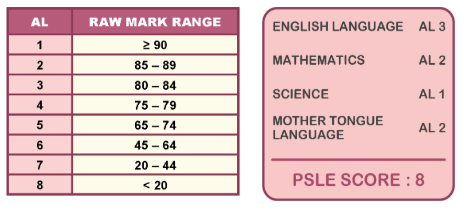
\includegraphics[width=0.5\paperwidth]{C:/Users/Admin/Desktop/Github/question_bank/LyX/static/img/9597-DHS-2019-P1-Q3}
\par\end{center}

Secondary 1 posting will continue to be based on academic merit, using
the PSLE Score. 

Each student will submit a list of 6 schools in order of preference.
If two students with the same score are being considered for the last
place in a school, the following tie-breakers will be used: 
\begin{itemize}
\item Citizenship - priority given to Singapore Citizens (SC), then Singapore
Permanent Residents (PR), then International Students (IS) 
\item Choice order of schools - priority given to the student who indicates
a certain school as a higher choice 
\item Computerised balloting 
\end{itemize}
The file \texttt{PSLE21.txt} contains the application information
of 400 Primary 6 students of a primary school with the following structure:

\texttt{<StudentID>,<EnglishLanguageMark>,<MathematicsMark>,<ScienceMark>,<MotherTongueLangueMark>,<Citizenship>,<SchoolChoice1>,<SchoolChoice2>
,<SchoolChoice3> }

You may assume that in this school all students study subjects at
the standard level. Also, all of them have made up their mind to only
apply to 3 schools of their choice. If a student is unable to get
admission to a school of their choice, they will be posted to SchoolD.

It is decided to process and store the following application information
about the student in 4 linked lists. Each linked list pertain to the
vacancy positions of the 4 schools. Schools A, B and C have 120, 150
and 80 available places. The data to be stored in each linked list
node include: PSLE score, student ID, citizenship and the 3 school
choices. 

\subsection*{Task 3.1 }

Write program code to read in and store the contents of the file \texttt{PSLE21.txt}
in a dictionary \texttt{students} with key \texttt{StudentID} and
value the computed PSLE score, citizenship and three school choices.
Display the first 10 dictionary entries in \texttt{students}. 

\subsection*{Evidence 11}

Program code. \hfill{}{[}6{]}

\subsection*{Evidence 12 }

Screenshot for first 10 dictionary entries in \texttt{students}.\hfill{}
{[}1{]}

\subsection*{Task 3.2 }

Using OOP where appropriate, write program code to declare and initialise
the necessary classes. Insert the 400 students from the \texttt{students}
dictionary in Task 3.1 to the appropriate linked lists in your main
program driver code. 

\subsection*{Evidence 13 }

Program code. \hfill{}{[}16{]}

\subsection*{Evidence 14 }

Screenshots for the first 5 entries in each linked list. \hfill{}{[}4{]}

\subsection*{Task 3.3 }

Students \texttt{P351} and \texttt{P365} who were previously Singapore
Permanent Residents (PR) have successfully become Singapore Citizens
(SC). Write the necessary program code to update their citizenship
status and new secondary 1 posting order. 

\subsection*{Evidence 15}

Program code. \hfill{}{[}5{]}

\subsection*{Evidence 16 }

Screenshots. \hfill{}{[}2{]}

\subsection*{Task 3.4}

Student \texttt{P286} has decided to emigrate to another country with
his/her parents. Write the necessary program code to remove him/her
from his/her existing allocation and perform the necessary adjustments
to fill up the vacancy. 

\subsection*{Evidence 17}

Program code. \hfill{}{[}5{]}

\subsection*{Evidence 18 }

Screenshot.\hfill{} {[}1{]}

 \newpage 

\item \textbf{{[}DHS/PRELIM/9597/2019/P1/Q4{]} }

The Viola-Jones object detection algorithm, named after two computer
vision researchers Paul Viola and Michael Jones, uses integral images
to detect the presence of facial features in an image efficiently. 

An integral image (also known as a summed-area table) is the name
of both a data structure and an algorithm used to obtain this data
structure. It uses a quick and efficient way to calculate the sum
of pixel values in a rectangular part of an image. 

In an integral image, the value of each point is the sum of all pixels
above and to the left, including the target pixel: 
\begin{center}
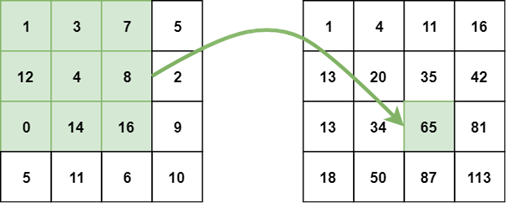
\includegraphics[width=0.5\paperwidth]{C:/Users/Admin/Desktop/Github/question_bank/LyX/static/img/9597-DHS-2019-P1-Q4-1}
\par\end{center}

The integral image can be calculated in a single pass over the original
image. This reduces summing the pixel intensities within a rectangle
into only three operations with four numbers, regardless of rectangle
size: 
\begin{center}
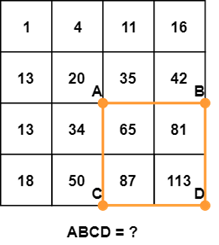
\includegraphics[width=0.25\paperwidth]{C:/Users/Admin/Desktop/Github/question_bank/LyX/static/img/9597-DHS-2019-P1-Q4-2}
\par\end{center}

The sum of pixels in the rectangle ABCD can be derived from the values
of points A, B, C, and D, using the formula $D-B-C+A$. It is easier
to understand this formula visually:

Note that subtracting both B and C means that the area defined with
A has been subtracted twice, so we need to add it back again. 

Thus $D-B-C+A=113-50-42+20=41$. 
\begin{center}
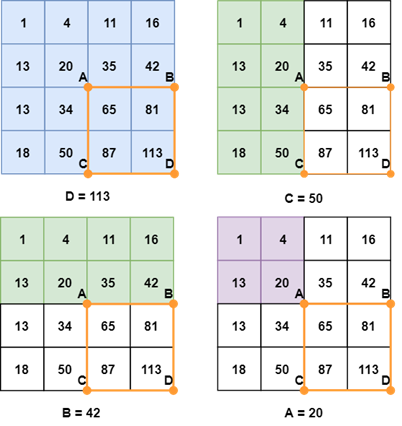
\includegraphics[width=0.5\paperwidth]{C:/Users/Admin/Desktop/Github/question_bank/LyX/static/img/9597-DHS-2019-P1-Q4-3}
\par\end{center}

\subsection*{Task 4.1 }

Write an \texttt{integral\_image()} function which reads in the data
from the file \texttt{IMAGE1.IN} into a 2D array and computes and
outputs the integral image to a file \texttt{IMAGE1.OUT} using the
algorithm described above, and also displays the result of $D-B-C+A$
to the screen. 

\subsection*{Evidence 19}

Program code. \hfill{} {[}13{]}

\subsection*{Evidence 20}

Screenshots of \texttt{IMAGE1.OUT} and output of $D-B-C+A$. \hfill{}{[}2{]}

\subsection*{Task 4.2}

Write a \texttt{magic()} function which is a generalisation of your
\texttt{integral\_image()} function which will work for any $m\times n$
rectangular 2D array and any rectangle ABCD.

Programmatically randomise your image with suitable values ($m,n\geq8$)
in \texttt{IMAGE2.IN} and work your magic on this pseudo-randomly
generated file to produce \texttt{IMAGE2.OUT} and the updated computed
value of $D-B-C+A$. 

\subsection*{Evidence 21}

Program code. \hfill{}{[}13{]}

\subsection*{Evidence 22 }

Screenshots of \texttt{IMAGE2.OUT} and output of $D-B-C+A$. \hfill{}{[}2{]}

 \newpage 

\item \textbf{{[}DHS/PRELIM/9597/2019/P2/Q1{]} }

The following Gantt chart shows the key tasks involved in a data science
project for a product recommendation engine based on customers' past
purchase patterns.
\noindent \begin{center}
\begin{tabular}{|c|l|c|c|c|c|c|c|c|c|c|c|c|c|c|c|c|c|c|c|c|c|c|}
\hline 
AID & Activity & \multicolumn{21}{c|}{Week}\tabularnewline
\hline 
A & Understand the problem & X & X &  &  &  &  &  &  &  &  &  &  &  &  &  &  &  &  &  &  & \tabularnewline
\hline 
B & Review with team &  &  & X &  &  &  &  &  &  &  &  &  &  &  &  &  &  &  &  &  & \tabularnewline
\hline 
C & Make problem statement &  &  & X &  &  &  &  &  &  &  &  &  &  &  &  &  &  &  &  &  & \tabularnewline
\hline 
D & Define scope of work &  &  & X &  &  &  &  &  &  &  &  &  &  &  &  &  &  &  &  &  & \tabularnewline
\hline 
E & Identify suitable algorithms &  &  &  & X &  &  &  &  &  &  &  &  &  &  &  &  &  &  &  &  & \tabularnewline
\hline 
F & Collect data &  &  & X & X & X & X & X & X &  &  &  &  &  &  &  &  &  &  &  &  & \tabularnewline
\hline 
G & Clean data &  &  & X & X & X & X & X & X &  &  &  &  &  &  &  &  &  &  &  &  & \tabularnewline
\hline 
H & Exploratory data analysis &  &  &  &  & X & X &  &  &  &  &  &  &  &  &  &  &  &  &  &  & \tabularnewline
\hline 
I & Develop use cases &  &  &  &  &  & X & X &  &  &  &  &  &  &  &  &  &  &  &  &  & \tabularnewline
\hline 
J & Present use cases &  &  &  &  &  &  &  & X &  &  &  &  &  &  &  &  &  &  &  &  & \tabularnewline
\hline 
K & Analyse full data &  &  &  &  &  &  &  &  & X & X & X &  &  &  &  &  &  &  &  &  & \tabularnewline
\hline 
L & Develop proof of concept &  &  &  &  &  &  &  &  &  &  &  & X & X & X &  &  &  &  &  &  & \tabularnewline
\hline 
M & Get customer approval &  &  &  &  &  &  &  &  &  &  &  &  &  &  & X &  &  &  &  &  & \tabularnewline
\hline 
N & Build final models &  &  &  &  &  &  &  &  &  &  &  &  &  &  &  & X & X & X &  &  & \tabularnewline
\hline 
O & Deploy models &  &  &  &  &  &  &  &  &  &  &  &  &  &  &  &  &  &  & X & X & \tabularnewline
\hline 
P & Sign off &  &  &  &  &  &  &  &  &  &  &  &  &  &  &  &  &  &  &  &  & X\tabularnewline
\hline 
\end{tabular}
\par\end{center}

A project manager often uses both PERT chart and Gantt chart to illustrate
and manage a project workflow. 
\begin{enumerate}
\item Give one benefit and one limitation of using a Gantt chart to depict
a project workflow?\hfill{} {[}2{]}
\item {}
\begin{enumerate}
\item Construct a PERT chart to depict the project work flow.\hfill{} {[}4{]}
\item State the critical path and the minimum project completion time. \hfill{}{[}2{]}
\item Explain and give an example of a dependent activity.\hfill{} {[}2{]}
\item Explain and give an example of a concurrent activity. \hfill{}{[}2{]}
\item Indicate in your PERT chart and justify a suitable dummy activity.
\hfill{}{[}2{]}
\item Give an example to show your understanding of float or slack time.\hfill{}
{[}2{]}
\end{enumerate}
\item The project manager needs to include a documentation activity and
a cybersecurity activity to the project. Justify the significance
of these activities and show how these can be included in your PERT
chart. Explain any implications to the critical path and projection
completion time. \hfill{}{[}5{]}
\item The project team would inadvertently have access to some restricted
customer purchase information. Give two ethical considerations related
to the privacy of data and suggest possible mitigation measures.\hfill{}
{[}4{]}
\end{enumerate}
The following shows sample interaction snippets of an interactive
exploratory data analysis session. 
\begin{center}
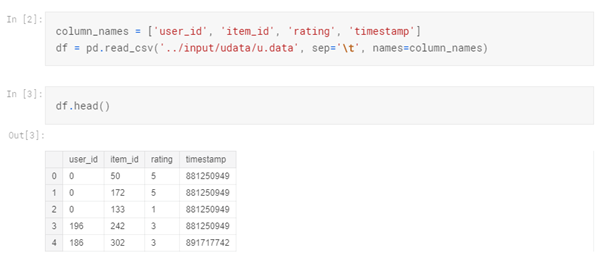
\includegraphics[width=0.65\paperwidth]{C:/Users/Admin/Desktop/Github/question_bank/LyX/static/img/9597-DHS-2019-P2-Q1-1}
\par\end{center}

\begin{center}
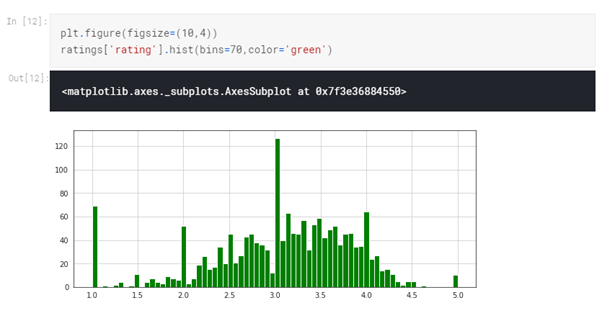
\includegraphics[width=0.65\paperwidth]{C:/Users/Admin/Desktop/Github/question_bank/LyX/static/img/9597-DHS-2019-P2-Q1-2}
\par\end{center}
\begin{enumerate}
\item[(e)]  {}
\begin{enumerate}
\item State the interface used and justify why this is the most appropriate
form of user interaction. \hfill{}{[}3{]}
\item The data analysis team is deciding on whether to perform the analysis
online in a cloud infrastructure or to process all data on a local
computer. What are two factors to consider in arriving at this decision?
\hfill{}{[}2{]}
\item Evaluate the pros and cons of each approach and make a recommendation
with reason(s) to the project team. \hfill{}{[}5{]}
\end{enumerate}
\item[(f)]  Given the relationship: bit rate = baud rate {*} voltage (\# bits
per signal)
\begin{enumerate}
\item Explain the difference between baud rate and bit rate. \hfill{}{[}2{]}
\item The following voltage levels expressed in volts are chosen to encode
bits:

-6.0, -4.5, -3.0, -1.5, +1.5, +3.0, +4.5, +6.0

How many bits represent these voltages?\hfill{} {[}1{]}
\item For the above voltages, write down one possible set of corresponding
bit patterns.\hfill{} {[}1{]}
\item If the baud rate of the line is 900 baud what is the bit rate for
the voltage levels?\hfill{} {[}1{]}
\end{enumerate}

 \newpage 

\end{enumerate}
\item \textbf{{[}DHS/PRELIM/9597/2019/P2/Q2{]} }
\begin{enumerate}
\item Given an array of integers, devise an algorithm for a function \texttt{FindLargest}
that arranges them in order to return the largest possible integer.
For example, given {[}10, 7, 76, 415{]}, your algorithm should return
77641510.\hfill{} {[}5{]}
\item Given an array of integers, devise an algorithm for a function \texttt{MultiplyNotMe}
that returns a new array such that each element at index i of the
new array is the product of all the numbers in the original array
except the one at i. For example, given {[}1, 2, 3, 4, 5{]}, your
algorithm should return {[}120, 60, 40, 30, 23{]}.\hfill{} {[}5{]}
\end{enumerate}

 \newpage 

\item \textbf{{[}DHS/PRELIM/9597/2019/P2/Q3{]} }
\begin{enumerate}
\item Given a binary search tree of positive integers, devise an algorithm
\texttt{FindFloorCeiling} to find the floor and ceiling of a given
positive integer k. The floor Is the highest element in the tree less
than or equal to an integer, while the ceiling is the lowest element
in the tree greater than or equal to an integer. If either value does
not exist, return -1. \hfill{}{[}5{]}
\item Given a sorted array, devise an algorithm \texttt{MakeBalancedBST}
to convert it into a height-balanced binary search tree. \hfill{}{[}5{]}
\end{enumerate}

 \newpage 

\item \textbf{{[}DHS/PRELIM/9597/2019/P2/Q4{]} }

Blackjack is a two-player card game whose rules are as follows:
\begin{itemize}
\item The player and then the dealer are each given two cards. 
\item The player can then \textquotedbl hit\textquotedbl , or ask for
arbitrarily many additional cards, so long as their total does not
exceed 21. 
\item The dealer must then hit if their total is 16 or lower, otherwise
pass. 
\item Finally, the two compare totals, and the one with the greatest sum
not exceeding 21 is the winner.
\end{itemize}
For this problem, cards values are counted as follows: each card between
2 and 10 counts as their face value, face cards count as 10, and aces
count as 1. 
\begin{enumerate}
\item Express the above blackjack game flow using a program flowchart. \hfill{}{[}4{]}
\item Given perfect knowledge of the sequence of cards in the deck, devise
an efficient algorithm that maximises the player's score (i.e. wins
minus losses). \hfill{} {[}8{]}
\item Evaluate the efficiency of your algorithm for part (b). \hfill{}{[}3{]}
\end{enumerate}

 \newpage 

\item \textbf{{[}DHS/PRELIM/9597/2019/P2/Q5{]} }

A role playing game (RPG) uses object-oriented programming (OOP) to
store its game characters' data. A character, either a hero or a monster,
has a name, health, magic points and inventory. Each character also
has a \texttt{take\_damage()} and a \texttt{display()} method. 

The game also has a special type of character, a dragon, which also
has additional data \texttt{airSpeed} and \texttt{breathType}.
\begin{enumerate}
\item Draw a class diagram showing the relationship between the different
game characters. \hfill{}{[}4{]}
\item Using appropriate examples, explain the following terms:
\begin{enumerate}
\item encapsulation
\item inheritance
\item polymorphism \hfill{}{[}6{]}
\end{enumerate}
\item Using suitable examples, explain why OOP is a preferred programming
paradigm in game development than a(n) imperative/procedural one.
\hfill{} {[}2{]}
\end{enumerate}

 \newpage 

\item \textbf{{[}DHS/PRELIM/9597/2019/P2/Q6{]} }

BuildingBloCS is Singapore's first/only/largest by Computing students
for Computing students and beyond national Computing education outreach
programme. In 2019, it comprises a series of workshops, talks, games,
projects showcase, programming quizzes, lucky draws and more (media
and entertainment very important). 

The organisers would like to apply what they learned in Computing
to manage workshop information using a relational database. 
\begin{itemize}
\item Each participant can register for one or more workshops 
\item Each workshop is conducted by one or more instructors 
\item Each workshop is also facilitated by one or more facilitators 
\end{itemize}
Due to Personal Data Protection Act (PDPA), it is decided to use an
alternative unique identifier as the primary key instead of collecting
participants' NRICs/FINs.

The normalised design requires a number of tables.
\begin{enumerate}
\item Draw an Entitiy-Relationship (E-R) diagram that shows these tables
and the relationships between them. \hfill{} {[}4{]}
\item Suggest and justify a suitable primary key candidate other than NRIC/FIN.
\hfill{} {[}2{]}
\item A table description can be expressed as:

\texttt{TableName(Attribute1, Attribute2, Attribute3, \dots )}

The primary key is indicated by underlining one or more attributes.

Derive the table descriptions for the tables. \hfill{}{[}6{]}
\item There are some fields with missing or null values. Explain how these
arise and how a Database Management System (DBMS) may provide facilities
to ensure the information is appropriately managed. \hfill{}{[}3{]}
\end{enumerate}

 \newpage 

\item \textbf{{[}HCI/PRELIM/9597/2019/P1/Q1{]} }

The manager of a private carpark wants to process the daily data of
people using the carpark. The carpark is open from 8am to 11pm and
the carpark charge is as follows:
\begin{itemize}
\item Before 5pm: \$1.50 per hour or part thereof 
\item After 5pm, \$3.00 per entry regardless of the duration
\end{itemize}
However, if a car enters before 5pm and leaves after 5pm, the charge
involves both rules. For example, if the car stays in the carpark
from 2.45pm to 6.30pm, it is broken down to 2 hours 15 minutes before
5pm and 1 hour 30 minutes after 5pm. Hence the charge will be \$1.50
{*} 3 + \$3.00 = \$7.50. 

Each day the carpark electronic system generates a file\texttt{ CARPARK.txt}.
Each record in the file has the following format:
\noindent \begin{center}
\texttt{<CARPLATE NUMBER>,<START TIME>,<END TIME>}
\par\end{center}

For example, \texttt{SLX2315A,0940,1415} means that a car with car
plate number SLX2315A entered the carpark at 9.40am and left at 2.15pm. 

You are \textbf{not} allowed to use any built-in functions for time
processing. 

\subsection*{Task 1.1 }

Write program code for the \texttt{Price} function using the following
specification:
\noindent \begin{center}
\texttt{FUNCTION Price (start: STRING, end: STRING) : FLOAT}
\par\end{center}

The function has two string parameters \texttt{start}, \texttt{end}
which refers to the start and end time when the car parked. The function
returns the carpark charge as a float. 

\subsection*{Evidence 1 }

Your program code.\hfill{} {[}5{]}

\subsection*{Task 1.2 }

Write a program code to perform the following task for the manager:
\begin{itemize}
\item Read data from \texttt{CARPARK.txt }
\item Write all the car plate numbers and corresponding carpark charges
to another file \texttt{CHARGE.txt}, in the following format: 
\noindent \begin{center}
\texttt{<CARPLATE NUMBER>,<CARPARK CHARGE>}
\par\end{center}

\noindent \begin{center}
\texttt{<CARPLATE NUMBER>,<CARPARK CHARGE>}
\par\end{center}
\item Output the total charges for the day
\end{itemize}

\subsection*{Evidence 2 }

Your program code.\hfill{} {[}7{]}

\subsection*{Evidence 3}

One screenshot showing the program output and contents of \texttt{CHARGE.txt}
from running the program.\hfill{} {[}3{]}

 \newpage 

\item \textbf{{[}HCI/PRELIM/9597/2019/P1/Q2{]} }

When a list of integers has repeated numbers, the searching and sorting
algorithms can be different. The task is to perform an insertion sort
before a binary search is executed. 

\subsection*{Task 2.1 }

Write the program code for a procedure to implement insertion sort
in ascending order. The input parameter is a list of integers which
may have repeated numbers. 

\subsection*{Evidence 4}

Your program code.\hfill{} {[}4{]}

\subsection*{Task 2.2 }

Write the program code for a procedure to implement binary search
for a targeted integer. The input parameter is an ordered list of
integers which may have repeated numbers. The procedure outputs all
the indices at which the target appears, or \texttt{\textminus 1}
if the target is not found. 

\subsection*{Evidence 5 }

Your program code. \hfill{}{[}9{]}

\subsection*{Task 2.3 }

The file \texttt{NUMBERS.txt} contains one integer at each line. Write
a program that uses the procedures in previous tasks and performs
the following task: 
\begin{itemize}
\item Reads the text file \texttt{NUMBERS.txt}, 
\item Perform insertion sort, and outputs the list of integers in a row, 
\item Prompts the user to provide a target to be searched, 
\item Perform a binary search and output an appropriate message
\end{itemize}

\subsection*{Evidence 6 }

Your program code.\hfill{} {[}4{]}

\subsection*{Task 2.4 }

Draw up \textbf{three} suitable tests and provide screenshot evidence
for your testing. 

\subsection*{Evidence 7 }

Annotated screenshots for each test data run. \hfill{}{[}3{]}

 \newpage 

\item \textbf{{[}HCI/PRELIM/9597/2019/P1/Q3{]} }

The examinations department of a school needs to keep long-term records
of the overall examination achievements of its students.

Students at the school have two main choices. Firstly, they can take
a variety of subjects and achieve an Academic Diploma. A diploma gives
them the opportunity to go to university. Secondly they can achieve
a Skills Certificate where they focus on one particular area (such
as IT). This gives them the necessary skills to start a career in
their chosen area.

The examinations department decides to store the following data:
\begin{itemize}
\item \texttt{StudID} is used to uniquely identify a particular student
and is six digits. The first four digits represent the year that the
student started at the school and the last two digits are used to
make the \texttt{StudID} unique e.g. 201804.
\item \texttt{Name} is the name of the student and is at most 30 characters.
\item \texttt{StudType} is the type of student and can have the values \textquoteleft D\textquoteright{}
or \textquoteleft S\textquoteright .
\item \texttt{SkillArea} is text and gives the area that the student acquired
skills in. It can have one of three values: \textquoteleft IT\textquoteright ,
\textquoteleft Business\textquoteright{} or \textquoteleft Accountancy\textquoteright .
\item \texttt{NoOfSub} is the number of subjects studied by those taking
the Diploma. 
\item \texttt{Result} is a single character and is used to indicate the
overall grade awarded. For those students who took the Skills Certificate
the grades could be Distinction (D), Merit (M), Pass (P) or Fail (F).
For those who took the Diploma the grade could be one of the letters
A to F. Grade A to E are passes. Grade F is a fail.
\end{itemize}
The program design for a solution to this problem is to be implemented
with object-oriented programming with the following three classes:
\begin{center}
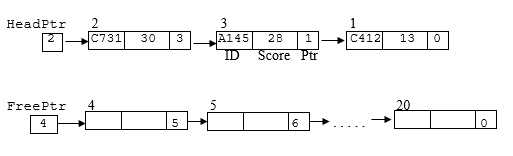
\includegraphics[width=0.5\paperwidth]{C:/Users/Admin/Desktop/Github/question_bank/LyX/static/img/9597-HCI-2019-P1-Q4-1}
\par\end{center}

\subsection*{Task 3.1 }

Write program code to define the classes \texttt{Student}, \texttt{Diploma}
and \texttt{SkillsCert}.

\subsection*{Evidence 8}

Program code for the three classes in Task 3.1. \hfill{}{[}6{]}

Assume that a file, \texttt{STUDENT.txt}, which contains details of
each student, has been created for you. The format of each student
record is as follows: 
\noindent \begin{center}
\texttt{<StudID>|<Name>|<StudType>|<SkillArea>|<NoOfSub>|<Result>}
\par\end{center}
\begin{itemize}
\item \texttt{SkillArea} would have the value \textquoteleft Diploma\textquoteright{}
if the student is taking a Diploma. 
\item \texttt{NoOfSub} would have the value 0 for those taking the Skills
Certificate.
\item \texttt{Result} is left blank initially. 
\end{itemize}

\subsection*{Task 3.2 }

Write a module, \texttt{ENTER\_RESULT}, which, when called, will ask
the user for a particular \texttt{StudID} whose result is to be entered.
Using the student ID that has been input, the corresponding student
record will be located in \texttt{STUDENT.txt}. The student data will
be displayed to the user. The user will be allowed to enter the result
for the student. The amended record will be stored back in \texttt{STUDENT.txt}. 

The student ID and result that have been input should be validated. 

If the \texttt{StudID} does not exist, the user will be given an appropriate
message.

\textbf{You are expected to make use of the classes you designed in
Task 3.1}.

Run the program \textbf{three} times. Use the following data input,
and produce a screenshot for each. 
\noindent \begin{center}
\begin{tabular}{cc}
StudID & Result\tabularnewline
\hline 
\texttt{201701} & \texttt{A}\tabularnewline
\texttt{201801} & \texttt{B}\tabularnewline
\texttt{201901} & \texttt{M}\tabularnewline
\end{tabular}
\par\end{center}

\subsection*{Evidence 9}

Program code for Task 3.2 \hfill{}{[}8{]}

\subsection*{Evidence 10 }

Three screenshots showing the test runs and final contents of \texttt{STUDENT.txt}
to show evidence that successful updates have been carried out. \hfill{}{[}2{]}

\subsection*{Task 3.3}

Implement code as specified below.

A report should be generated and displayed which will list the students
whose result has still not been entered into the \texttt{STUDENT.txt}
file. The report will list, for each different starting year: 
\begin{itemize}
\item \texttt{StudID} 
\item \texttt{Name} 
\item \texttt{StudType}
\item \texttt{SkillArea} or \texttt{NoOfSub} depending upon the value of
\texttt{StudType} 
\end{itemize}
In addition the number of each student type for each year will also
be output.

A sample output is shown below.
\noindent \begin{center}
\begin{tabular}{llll}
Year: 2017 &  &  & \tabularnewline
\hline 
\texttt{201715} & FLoo & D & 6\tabularnewline
\texttt{201708} & BLang & D & 5\tabularnewline
\texttt{201710} & LArms & S & IT\tabularnewline
Diplomas: & 2 &  & \tabularnewline
Skills: & 1 &  & \tabularnewline
\end{tabular}
\par\end{center}

\noindent \begin{center}
\begin{tabular}{llll}
Year: 2018 &  &  & \tabularnewline
\hline 
\texttt{201813} & FJean & D & 7\tabularnewline
\texttt{201817} & ABright & D & 7\tabularnewline
Diplomas: & 2 &  & \tabularnewline
Skills: & 0 &  & \tabularnewline
\end{tabular}
\par\end{center}

\noindent \begin{center}
\begin{tabular}{llll}
Year: 2019 &  &  & \tabularnewline
\hline 
\texttt{201905} & Alfie & S & Business\tabularnewline
\texttt{201903} & GKoh & D & 8\tabularnewline
Diplomas: & 1 &  & \tabularnewline
Skills: & 1 &  & \tabularnewline
\end{tabular}
\par\end{center}

\subsection*{Evidence 11 }

Program code for Task 3.3. \hfill{}{[}8{]}

\subsection*{Evidence 12 }

Screenshot of the output produced.\hfill{} {[}2{]}

 \newpage 

\item \textbf{{[}HCI/PRELIM/9597/2019/P1/Q4{]} }

A game maintains the player IDs and their scores in an ordered linked
list. The player with the highest score is stored at the first node
while the player with the lowest score is stored at the last node. 

The program to implement the linked list abstract data type will use
two classes, \texttt{ListNode} and \texttt{LinkedList}. 

The \texttt{ListNode} class has the following properties:
\noindent \begin{center}
\begin{tabular}{|l|l|l|}
\hline 
\texttt{\hspace{0.01\columnwidth}}Identifier & \texttt{\hspace{0.01\columnwidth}}Data Type & \texttt{\hspace{0.05\columnwidth}}Description\tabularnewline
\hline 
\texttt{ID} & \texttt{STRING} & The ID of the player. All IDs are unique and have the format \texttt{L999}
where \texttt{L} is any uppercase letter and \texttt{9} is a digit.\tabularnewline
\hline 
\texttt{Score} & \texttt{INTEGER} & The score of the player.\tabularnewline
\hline 
\texttt{Ptr} & \texttt{INTEGER} & The pointer to the next node.\tabularnewline
\hline 
\end{tabular}
\par\end{center}

The \texttt{LinkedList} class has the following properties: 
\noindent \begin{center}
\begin{tabular}{|l|l|l|}
\hline 
\texttt{\hspace{0.01\columnwidth}}Identifier & \texttt{\hspace{0.01\columnwidth}}Data Type & \texttt{\hspace{0.05\columnwidth}}Description\tabularnewline
\hline 
\texttt{Node} & \texttt{ARRAY{[}1..20{]} OF ListNode} & 1-D array stores the nodes that make the ordered linked list. The
unused nodes are linked together into a free list.\tabularnewline
\hline 
\texttt{HeadPtr} & \texttt{INTEGER} & Pointer to the first node in the ordered list.\tabularnewline
\hline 
\texttt{FreePtr} & \texttt{INTEGER} & Pointer to the first node in the free list.\tabularnewline
\hline 
\end{tabular}
\par\end{center}

The following diagram shows an example of a linked list object. This
example list consists of three nodes, linked in descending order of
the game scores. The unused nodes are linked to form a free list.
\begin{center}
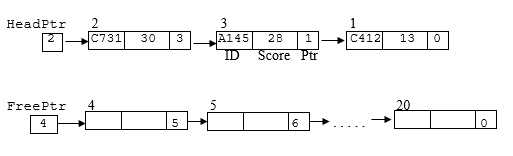
\includegraphics[width=0.5\paperwidth]{C:/Users/Admin/Desktop/Github/question_bank/LyX/static/img/9597-HCI-2019-P1-Q4-1}
\par\end{center}

\subsection*{Task 4.1}

Write program code for the classes \texttt{ListNode} and \texttt{Linkedlist}
to declare all the required variables and create the initial empty
linked list which contains all 20 nodes.

Add statement(s) to initialise the empty ordered linked list.

\subsection*{Evidence 13 }

Your program code for Task 4.1. \hfill{}{[}6{]}

\subsection*{Task 4.2 }

Write code to implement a method \texttt{AddInOrder} that will add
a new node with player\textquoteright s ID and score into the ordered
linked list in descending order of the scores. Node added to the ordered
linked list should be taken from the free list. 

Assume that all players have different scores.

\subsection*{Evidence 14 }

Your program code for Task 4.2.\hfill{} {[}7{]}

\subsection*{Task 4.3 }

Write a procedure \texttt{OutputData} which displays the value of
\texttt{HeadPtr}, the value of \texttt{FreePtr} and the contents of
\texttt{Node} array in index order.

\subsection*{Evidence 15 }

Your program code for Task 4.3.\hfill{} {[}3{]}

The files \texttt{SCORES1.txt} and \texttt{SCORES2.txt} contain the
game data. Each entry has the following format: \texttt{<Player ID>,<Score>} 

\subsection*{Task 4.4 }

Write a main program to:
\begin{itemize}
\item Create a linked list object 
\item Read all player data from \texttt{SCORES1.txt} and add them to the
linked list by calling procedure \texttt{AddInOrder}. 
\item Your program will then call procedure \texttt{OutputData}.
\end{itemize}

\subsection*{Evidence 16 }

Screenshot showing the output from running the program in Task 4.4
using \texttt{SCORES1.txt} file. \hfill{}{[}2{]}

\subsection*{Task 4.5 }

Amend your \texttt{AddInOrder} program code in Task 4.2 so that if
two or more players have the same score, they are stored in alphabetical
player ID order. Use the file \texttt{SCORES2.txt} to test your program
code.

The following diagram shows an example of an ordered linked list where
players \texttt{C412} and \texttt{B321} have the same game score of
\texttt{13} points. 
\begin{center}
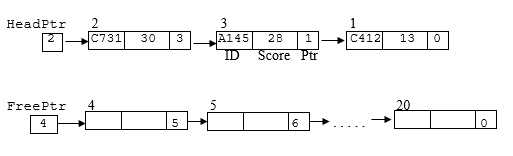
\includegraphics[width=0.5\paperwidth]{C:/Users/Admin/Desktop/Github/question_bank/LyX/static/img/9597-HCI-2019-P1-Q4-1}
\par\end{center}

\subsection*{Evidence 17 }

The amended program code for method \texttt{AddInOrder}. \hfill{}{[}4{]}

\subsection*{Evidence 18}

Screenshot showing the output from running the program in Task 4.4
using \texttt{SCORES2.txt} file. \hfill{}{[}2{]}

\subsection*{Task 4.6 }

A method \texttt{DisplayByRank} is to be added, which outputs all
player IDs and their scores stored in the ordered linked list in rank
order. If multiple players record the same score, they will have the
same rank. 

Below is a sample of screen output:
\noindent \begin{center}
\begin{tabular}{lll}
\texttt{Rank} & \texttt{Player ID} & \texttt{Score}\tabularnewline
\texttt{1} & \texttt{F111} & \texttt{45}\tabularnewline
\texttt{1} & \texttt{G333} & \texttt{45}\tabularnewline
\texttt{1} & \texttt{Z333} & \texttt{45}\tabularnewline
\texttt{4} & \texttt{C333} & \texttt{38}\tabularnewline
\texttt{5} & \texttt{B111} & \texttt{25}\tabularnewline
\texttt{5} & \texttt{Q333} & \texttt{25}\tabularnewline
\texttt{7} & \texttt{E333} & \texttt{12}\tabularnewline
\end{tabular}
\par\end{center}

Write program code to:
\begin{itemize}
\item Implement this method 
\item Test the program code with the data from Task 4.5.
\end{itemize}

\subsection*{Evidence 19 }

Program code for Task 4.6. \hfill{}{[}7{]}

\subsection*{Evidence 20}

Screenshot of the program output.\hfill{} {[}2{]}

\subsection*{Task 4.7 }

Write a recursive \texttt{ReverseTraversal} procedure that will traverse
the linked list in reverse order and output players\textquoteright{}
IDs and scores in ascending scores order.

Include a call to the procedure from your main program.

Test the program code with the data from Task 4.5.

\subsection*{Evidence 21 }

Your program code for Task 4.7.\hfill{}{[}4{]}

\subsection*{Evidence 22}

Screenshot showing the program execution to test the \texttt{ReverseTraversal}
method. \hfill{}{[}2{]}

 \newpage 

\item \textbf{{[}HCI/PRELIM/9597/2019/P1/Q8{]} }

Using the following numbers as an example, show how the numbers can
be sorted in ascending order using a \textbf{quick sort}. For each
pass, show the numbers swapped and the sub lists after splitting. 
\noindent \begin{center}
435, 646, 344, 54, 23, 98
\par\end{center}

\noindent \begin{flushleft}
\hfill{}{[}7{]}
\par\end{flushleft}

 \newpage 

\item \textbf{{[}HCI/PRELIM/9597/2019/P2/Q1{]} }

A bookshop wishes to expand its business from a brick and mortar shop
to allow for online sales. A software company has been engaged by
the bookshop to develop the online sales system. 
\begin{enumerate}
\item The analyst decides to adopt a top-down approach to the design. What
are the advantages of using top-down design to solve complex problems?\hfill{}
{[}3{]} 
\end{enumerate}
The project manager decides to use some project management tool in
the planning of the project. Below is the list of activities along
with their required time for completion.
\noindent \begin{center}
\begin{tabular}{|c|c|c|}
\hline 
Activity & Expected completion time (day) & Preceded by\tabularnewline
\hline 
\hline 
A & 2 & -\tabularnewline
\hline 
B & 3 & A\tabularnewline
\hline 
C & 1 & B\tabularnewline
\hline 
D & 3 & B\tabularnewline
\hline 
E & 4 & C\tabularnewline
\hline 
F & 3 & D\tabularnewline
\hline 
G & 2 & A\tabularnewline
\hline 
H & 5 & G\tabularnewline
\hline 
I & 3 & E, F, H\tabularnewline
\hline 
\end{tabular}
\par\end{center}
\begin{enumerate}
\item[(b)]  Construct the PERT chart for the activities, indicating the earliest
start time and latest start time of each activity. \hfill{}{[}3{]}
\item[(c)]  Which tasks are on the critical path of the Program Evaluation and
Review Technique (PERT) chart? \hfill{}{[}1{]}
\item[(d)]  What is the slack time for Task C and G? \hfill{}{[}2{]}
\item[(e)]  The person working on Task C tells the project manager he cannot
start work until one day after the scheduled starting date. What impact
would this have on the completion date of the project? Why?\hfill{}
{[}2{]}
\item[(f)]  Task A will be delayed by 2 days for some reason. If the project
manager still wants to finish the project within the original time
frame, he will need to shorten the time for one or more of the tasks.
What steps can he take to reduce the number of days allocated to a
task? \hfill{}{[}2{]}
\item[(g)]  The project manager decides to reduce the time needed for Tasks
D and F by one day each. How effective will this reduction be in achieving
his aim of maintaining the original finish time for the project? What
can he do for it to be more effective?\hfill{} {[}2{]}
\item[(h)]  Produce a Gantt chart based on the above information. \hfill{}{[}2{]}
\item[(i)]  Give \textbf{one} reason why a Gantt chart may be preferred over
a PERT chart.\hfill{} {[}1{]}
\end{enumerate}

 \newpage 

\item \textbf{{[}HCI/PRELIM/9597/2019/P2/Q2{]} }

Customers can view a catalogue of books and order from its website.
Payment is made by the customer forwarding their credit card details,
which are processed immediately. Details of the orders are matched
against the stock file to check for availability of items before packing
lists are produced and sent to the packing department.
\begin{enumerate}
\item Draw a data flow diagram to explain the flow of data through this
system.\hfill{} {[}6{]}
\item Using examples from your DFD, explain how the diagram helps to inform
a database solution for the new computerized system.\hfill{} {[}4{]}
\item Give \textbf{two} parts of the database design that is not possible
from the DFD. \hfill{}{[}2{]}
\end{enumerate}

 \newpage 

\item \textbf{{[}HCI/PRELIM/9597/2019/P2/Q3{]} }
\begin{enumerate}
\item Explain the difference between synchronous and asynchronous data transmission.\hfill{}
{[}2{]}
\item Describe the three modes of data transmission: simplex, half-duplex
and full-duplex. \hfill{}{[}3{]}
\item Give \textbf{two} advantages of packet switching over circuit switching.\hfill{}
{[}2{]}
\end{enumerate}

 \newpage 

\item \textbf{{[}HCI/PRELIM/9597/2019/P2/Q4{]} }

Sing Airline Company uses a website to provide ticket purchasing services
to customers. 
\begin{enumerate}
\item Customers are required to fill up a form with their name, passport
number, hand phone number and flight information. Give \textbf{two}
examples of data validation and \textbf{one} example of data verification
for the company to validate the customers\textquoteright{} data. \hfill{}
{[}3{]}
\item Explain the purpose of using client and server scripting and give
\textbf{one} scripting language for each. \hfill{} {[}4{]}
\item The company uses a web server to handle the customers\textquoteright{}
orders. Describe \textbf{two} possible threats that the web server
may encounter and suggest \textbf{one} strategy for each threat. \hfill{}
{[}4{]}
\item Due to large amount of information to maintain and protect, the company
is planning to use cloud computing to store and access data. Give
\textbf{one} advantage and \textbf{one} disadvantage of using this
technology. \hfill{}{[}2{]}
\item The company\textquoteright s staff handbook must include rules and
regulations for IT staff. Suggest \textbf{two} code of conduct for
the company. \hfill{} {[}2{]}
\end{enumerate}

 \newpage 

\item \textbf{{[}HCI/PRELIM/9597/2019/P2/Q5{]} }

Below is the manner in which the school library will process its overdue
list:
\begin{itemize}
\item If a book is overdue then a reminder letter would normally be sent.
\item However, if the book is more than 5 days overdue, 2 further checks
are made to see whether the reminder should be replaced by a warning
letter:
\begin{itemize}
\item If the student has had a previous warning letter the student will
not only receive the warning letter but, in addition, a copy will
be sent to the parents of the student.
\item If the student has more than 4 books overdue, but no previous warning
letter, the reminder letter is replaced by a warning letter.
\end{itemize}
\end{itemize}
\begin{enumerate}
\item Create a decision table showing all the possible outcomes and results.
\hfill{}{[}4{]}
\item Simplify your decision table by removing redundancies. \hfill{}{[}2{]}
\end{enumerate}

 \newpage 

\item \textbf{{[}HCI/PRELIM/9597/2019/P2/Q6{]} }

A company manages subscriptions to thirty different magazines. Customers
can subscribe to receive one or more of the magazines.
\begin{itemize}
\item Each magazine has a category such as Gardening or Current Affairs. 
\item Each magazine has a subscription rate, which is the cost of subscribing
to receive the magazine for 12 months.
\end{itemize}
Details of the subscriptions are to be stored in a flat file. 

\texttt{Magazine(MagazineID, MagazineName, Category, SubscriptionRate,
CustomerID, StartDate, EndDate, CustomerName, Address, PostCode, TelephoneNumber) }
\begin{enumerate}
\item What is the difference between a flat file and a relational database?
\hfill{} {[}2{]}
\item Identify and state \textbf{three} potential problems with the flat
file implementation for the magazine subscriptions. \hfill{}{[}3{]}
\item Improved on the flat file and determine the relations needed in the
relational database for the above. Explain the purpose of each relation.
\hfill{}{[}6{]}
\item In what way can your database solve the three problems in \textbf{part
(b)}. \hfill{} {[}3{]}
\item Draw the Entity-Relationship diagram between the relations you have
in \textbf{part (c)}. Explain your answer. \hfill{}{[}6{]}
\end{enumerate}

 \newpage 

\item \textbf{{[}HCI/PRELIM/9597/2019/P2/Q7{]} }

The algebraic expression \texttt{X = 2 {*} A + B} could be held in
a binary tree as:
\begin{center}
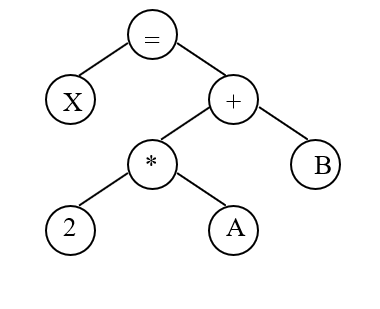
\includegraphics[width=0.5\paperwidth]{C:/Users/Admin/Desktop/Github/question_bank/LyX/static/img/9597-HCI-2019-P2-Q7}
\par\end{center}

This tree can then be read using the following algorithm:

process left subtree 

process right subtree 

read root node

This will give \texttt{X 2 A {*} B + =} which is the reverse Polish
form of the expression.
\begin{enumerate}
\item Using diagrams to help the explanation, or otherwise, show how a computer
can use a stack to evaluate the expression from its reverse Polish
form. \hfill{}{[}4{]}
\item The tree in the example could be stored in an array called TREE.
\noindent \begin{center}
\begin{tabular}{|c|c|c|c|}
\hline 
TREE{[}9{]} &  &  & \tabularnewline
\hline 
TREE{[}8{]} &  & -1 & \tabularnewline
\hline 
TREE{[}7{]} &  & 5 & \tabularnewline
\hline 
TREE{[}6{]} &  &  & \tabularnewline
\hline 
TREE{[}5{]} & 2 &  & \tabularnewline
\hline 
TREE{[}4{]} &  &  & \tabularnewline
\hline 
TREE{[}3{]} & X &  & \tabularnewline
\hline 
TREE{[}2{]} &  &  & \tabularnewline
\hline 
TREE{[}1{]} & B &  & \tabularnewline
\hline 
TREE{[}0{]} & = & 3 & 4\tabularnewline
\hline 
\end{tabular}
\par\end{center}

The values in each location in the array are: node value; left pointer;
right pointer. Where no left or right pointer exists the rouge value
-1 is used. Copy and complete the array for the example. (Note that,
since in the example there are only seven nodes, three rows of the
array will be unused.) \hfill{}{[}5{]}
\item Draw a tree similar to the one in the example which would represent
the expression:
\begin{center}
\texttt{Y = 2 {*} (A + B) \textendash{} (A \textasciicircum{} 2)} 
\par\end{center}

where \texttt{x \textasciicircum{} y} means $\mathtt{x^{y}}$.\hfill{}{[}3{]}
\item Using the algorithm in the example, and your tree, write out the reverse
Polish form of the expression in \textbf{part} (c). \hfill{}{[}3{]}
\end{enumerate}

 \newpage 

\item \textbf{{[}JPJC/PRELIM/9597/2019/P1/Q1{]} }

The file \texttt{VISITORS.txt} contains the number of visitors to
Singapore from 1978 to 2018. Each line of the text file is in the
following format: 
\noindent \begin{center}
\texttt{<year>,<month>,<number\_of\_visitors> }
\par\end{center}

\subsection*{Task 1.1 }

Write program code to 
\begin{itemize}
\item read the data from the file and store them in an appropriate data
structure, 
\item get user input to select the \textbf{year(s)} to display for \textbf{total
number of visitors}, 
\item ensure that user input for\textbf{ start year} and \textbf{end year}
are valid, 
\item display the \textbf{year(s)} and \textbf{number of visitors}. 
\end{itemize}
Sample output: 

\noindent\fbox{\begin{minipage}[t]{1\columnwidth - 2\fboxsep - 2\fboxrule}%
\texttt{Start year : 1978}

\texttt{End year ~~: 1980}

\texttt{Year Number of visitors }

\texttt{1978 1234567 }

\texttt{1979 1542384 }

\texttt{1980 1278652 }%
\end{minipage}}

\subsection*{Evidence 1 }

Your program code. \hfill{}{[}11{]}

\subsection*{Task 1.2 }

Test your program with \textbf{four} relevant test data for user input.
Copy the table with the following headings to show your test cases. 
\noindent \begin{center}
\begin{tabular}{|c|c|c|}
\hline 
Test data & Purpose of test data & Expected results \tabularnewline
\hline 
 &  & \tabularnewline
\hline 
\end{tabular} 
\par\end{center}

\subsection*{Evidence 2 }

Completed table with \textbf{four} test cases. 

Screenshots of running your program with the \textbf{four} test cases.
\hfill{}{[}4{]}

 \newpage 

\item \textbf{{[}JPJC/PRELIM/9597/2019/P1/Q2{]} }

The incomplete pseudocode function below takes in an array as input.
The array will then be sorted in ascending order and the results will
be returned. Note that the start index of the array is 1. 

\noindent %
\noindent\begin{minipage}[t]{1\columnwidth}%
\texttt{FUNCTION SomeSort(SomeList : ARRAY) }

\texttt{\qquad{}FOR Pointer \textleftarrow{} 2 TO NumberOfItems }

\texttt{\qquad{}\qquad{}ItemToBeInserted \textleftarrow{} SomeList{[}Pointer{]} }

\texttt{\qquad{}\qquad{}CurrentItem \textleftarrow{} Pointer \textendash{}
1 }

\texttt{\qquad{}\qquad{}WHILE(SomeList{[}CurrentItem{]}>ItemToBeInserted
AND CurrentItem>0) }

\texttt{\qquad{}\qquad{}\qquad{}SomeList{[}CurrentItem+1{]} \textleftarrow{}
SomeList{[}CurrentItem{]} }

\texttt{\qquad{}\qquad{}\qquad{}CurrentItem \textleftarrow{} CurrentItem
- 1 }

\texttt{\qquad{}\qquad{}ENDWHILE}

\texttt{\qquad{}\qquad{}............... $\mathtt{A}$............... }

\texttt{\qquad{}ENDFOR }

\texttt{\qquad{}RETURN ARRAY}

\texttt{ENDFUNCTION }%
\end{minipage}

\subsection*{Task 2.1 }

Complete the missing line and write program code to implement the
complete function. Sort the array given in the file \texttt{NUMBERS.txt}.
You may copy and paste the array into your program code. 

\subsection*{Evidence 3 }
\begin{itemize}
\item Your program code. 
\item Screenshot showing the array before and after running the function.\hfill{}
{[}7{]}
\end{itemize}

\subsection*{Task 2.2 }

Write a bubble sort function that takes an array, sorts the array
and returns the array. 

\subsection*{Evidence 4 }

Your bubble sort function.\hfill{} {[}4{]}

\subsection*{Task 2.3 }

Amend your program code in both functions to count and display the
number of comparisons made when sorting the array. 

\subsection*{Evidence 5 }
\begin{itemize}
\item Your amended program code. 
\item Screenshot of running both sorting functions with number of comparisons
displayed.\hfill{} {[}4{]}
\end{itemize}

 \newpage 

\item \textbf{{[}JPJC/PRELIM/9597/2019/P1/Q3{]} }

JP Medical Centre uses a priority queue to register patients who visit
for medical attention. Upon registration at the medical centre, each
patient will be assigned a priority number according to the urgency
in seeking medical care. The urgent cases receive top priority and
go directly to the front of the queue, whereas the minor cases are
added to the bottom of the queue.

A priority queue is an extension of queue with the following properties.
\begin{itemize}
\item Every element has a priority associated with it. Higher priority has
a larger number. 
\item An element with high priority leaves the queue before an element with
low priority.
\item If two elements have the same priority, they are served according
to their order in the queue, i.e. the earlier element will be served
before the later element (FIFO). 
\end{itemize}
An example of operations on a priority queue is shown below:

\textbf{Initial state of priority queue} 

\begin{tabular}{|c|c|c|c|c|c|}
\hline 
Data & \textquoteleft jim\textquoteright{} & \textquoteleft ben\textquoteright{} & \textquoteleft ken\textquoteright{} & \textquoteleft wayne\textquoteright{} & \textquoteleft harry\textquoteright{}\tabularnewline
\hline 
Priority & 3 & 3 & 2 & 1 & 1\tabularnewline
\hline 
\multicolumn{1}{c}{} & \multicolumn{1}{c}{$\overset{\uparrow}{\boldsymbol{\text{front}}}$} & \multicolumn{1}{c}{} & \multicolumn{1}{c}{} & \multicolumn{1}{c}{} & \multicolumn{1}{c}{$\overset{\uparrow}{\boldsymbol{\text{rear}}}$}\tabularnewline
\end{tabular}

\textbf{Insert \textquoteleft jenny\textquoteright{} with priority
3:} \textquoteleft jenny\textquoteright{} joins the priority queue
ahead of \textquoteleft ken\textquoteright{} who has a priority of
2 

\begin{tabular}{|c|c|c|c|c|c|c|}
\hline 
Data & \textquoteleft jim\textquoteright{} & \textquoteleft ben\textquoteright{} & '\emph{jenny}' & \textquoteleft ken\textquoteright{} & \textquoteleft wayne\textquoteright{} & \textquoteleft harry\textquoteright{}\tabularnewline
\hline 
Priority & 3 & 3 & \emph{3} & 2 & 1 & 1\tabularnewline
\hline 
\multicolumn{1}{c}{} & \multicolumn{1}{c}{$\overset{\uparrow}{\boldsymbol{\text{front}}}$} & \multicolumn{1}{c}{} & \multicolumn{1}{c}{} & \multicolumn{1}{c}{} & \multicolumn{1}{c}{} & \multicolumn{1}{c}{$\overset{\uparrow}{\boldsymbol{\text{rear}}}$}\tabularnewline
\end{tabular}

Remove from priority queue: \textquoteleft jim\textquoteright{} is
removed from front of priority queue 

\begin{tabular}{|c|c|c|c|c|c|}
\hline 
Data & \textquoteleft ben\textquoteright{} & '\emph{jenny}' & \textquoteleft ken\textquoteright{} & \textquoteleft wayne\textquoteright{} & \textquoteleft harry\textquoteright{}\tabularnewline
\hline 
Priority & 3 & \emph{3} & 2 & 1 & 1\tabularnewline
\hline 
\multicolumn{1}{c}{} & \multicolumn{1}{c}{$\overset{\uparrow}{\boldsymbol{\text{front}}}$} & \multicolumn{1}{c}{} & \multicolumn{1}{c}{} & \multicolumn{1}{c}{} & \multicolumn{1}{c}{$\overset{\uparrow}{\boldsymbol{\text{rear}}}$}\tabularnewline
\end{tabular}

A \textbf{priority queue} abstract data type (ADT) is to be \textbf{implemented}
as \textbf{a linked list} using object-oriented programming. Two classes
\texttt{Node} and \texttt{PQueue} have been identified. 
\begin{center}
\begin{tabular}{|l|l|l|}
\hline 
\multicolumn{3}{|c|}{\texttt{Class: Node}}\tabularnewline
\hline 
\texttt{\textbf{\hspace{0.01\columnwidth}}}\textbf{Identifier} & \texttt{\textbf{\hspace{0.01\columnwidth}}}\textbf{Data Type} & \texttt{\textbf{\hspace{0.05\columnwidth}}}\textbf{Description}\tabularnewline
\hline 
\multicolumn{3}{|l|}{\textbf{Properties}}\tabularnewline
\hline 
\texttt{Data} & \texttt{STRING} & The node data\tabularnewline
\hline 
\texttt{Priority} & \texttt{INTEGER} & Indicates priority of node. Higher value has higher priority.\tabularnewline
\hline 
\texttt{Pointer} & \texttt{INTEGER} & Pointer to next node in queue.\tabularnewline
\hline 
\end{tabular}
\par\end{center}

\begin{center}
\begin{tabular}{|l|l|l|}
\hline 
\multicolumn{3}{|c|}{\texttt{Class: PQueue}}\tabularnewline
\hline 
\texttt{\textbf{\hspace{0.01\columnwidth}}}\textbf{Identifier} & \texttt{\textbf{\hspace{0.01\columnwidth}}}\textbf{Data Type} & \texttt{\textbf{\hspace{0.05\columnwidth}}}\textbf{Description}\tabularnewline
\hline 
\multicolumn{3}{|l|}{\textbf{Properties}}\tabularnewline
\hline 
\texttt{ThisPQueue} & \texttt{ARRAY{[}10{]} OF Node} & The data for the priority queue.\tabularnewline
\hline 
\texttt{Front} & \texttt{INTEGER} & Index for front node of queue. \tabularnewline
\hline 
\texttt{Rear} & \texttt{INTEGER} & Index for rear node of queue. \tabularnewline
\hline 
\texttt{NextFree} & \texttt{INTEGER} & Index for the next unused node.\tabularnewline
\hline 
\multicolumn{3}{|l|}{\textbf{Methods}}\tabularnewline
\hline 
\multirow{2}{*}{Initialise} & \multirow{2}{*}{\texttt{PROCEDURE}} & \textbullet{} Create a new priority queue \tabularnewline
 &  & \textbullet{} Initialise \texttt{Front} and \texttt{Rear} to -1.\tabularnewline
\hline 
\multirow{3}{*}{\texttt{JoinPQueue (NewItem:STRING, Priority:INTEGER)}} & \multirow{3}{*}{\texttt{PROCEDURE}} & \textbullet{} Create a new node of Node class.\tabularnewline
 &  & \textbullet{} Assign \texttt{NewItem} and \texttt{Priority} passed
as parameters to the \texttt{Data} and \texttt{Priority} attribute
of \texttt{Node}.\tabularnewline
 &  & \textbullet{} Assign \texttt{Node} to the \texttt{PQueue} according
to the priority of the node.\tabularnewline
\hline 
\multirow{2}{*}{\texttt{LeavePQueue}} & \multirow{2}{*}{\texttt{FUNCTION}} & \textbullet{} Remove \texttt{Node} from \texttt{PQueue}.\tabularnewline
 &  & \textbullet{} Return the \texttt{data} attribute of \texttt{Node}. \tabularnewline
\hline 
\end{tabular}
\par\end{center}

The diagram shows the linked list with: 
\begin{itemize}
\item the elements \textquoteleft ben\textquoteright , \textquoteleft jenny\textquoteright ,
\textquoteleft ken\textquoteright , \textquoteleft wayne\textquoteright ,
\textquoteleft harry\textquoteright{} in the priority queue
\item the unused nodes linked together
\end{itemize}
\begin{center}
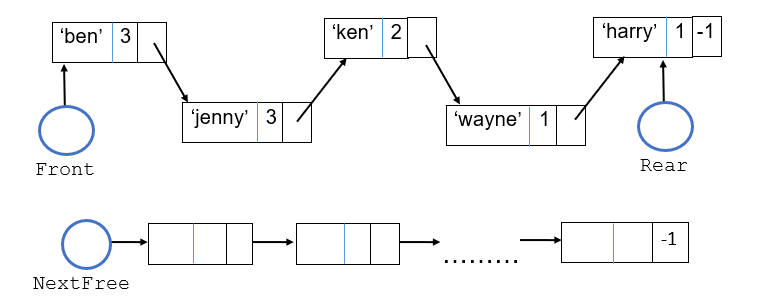
\includegraphics[width=0.65\paperwidth]{C:/Users/Admin/Desktop/Github/question_bank/LyX/static/img/9597-JPJC-2019-P1-Q3-1}
\par\end{center}

\subsection*{Task 3.1 }

Write program code to
\begin{itemize}
\item declare all the required identifiers for the \texttt{Node} and \texttt{PQueue}
class as specified, including the methods \texttt{Initialise}, \texttt{JoinPQueue},
\texttt{LeavePQueue}, and 
\item create the initial priority queue. 
\end{itemize}

\subsection*{Evidence 6: }

Your program code. \hfill{}{[}25{]}

\subsection*{Task 3.2 }

Write a procedure \texttt{OutputQueue} which displays the value of
\texttt{Front}, \texttt{Rear}, and \texttt{NextFree} and the contents
of \texttt{ThisPQueue} in index order. 

\subsection*{Evidence 7: }
\begin{itemize}
\item Your program code for \texttt{OutputPQueue}.
\item Screenshot for displaying the initial priority queue. \hfill{}{[}4{]}
\end{itemize}

\subsection*{Task 3.3 }

Write a main program to:
\begin{itemize}
\item Read from file\texttt{ PATIENTS.txt} all the data items with its priorities
into the priority queue by calling procedure \texttt{JoinPQueue}.
\item Output the priority queue by calling \texttt{OutputPQueue}. 
\end{itemize}

\subsection*{Evidence 8: }
\begin{itemize}
\item Your program code for task 3.3. 
\item Screenshot showing the output from running program in task 3.3. \hfill{}{[}5{]}
\end{itemize}
Task 3.4 

Write additional code in your main program that prints a menu with
the following options:

\noindent\fbox{\begin{minipage}[t]{1\columnwidth - 2\fboxsep - 2\fboxrule}%
\noindent \texttt{Patient Queue Menu }
\begin{enumerate}
\item[1)] \texttt{ Add patient to PQueue }
\item[2)] \texttt{ Remove patient from PQueue }
\item[3)] \texttt{ Display PQueue }
\item[4)] \texttt{ Exit program }
\end{enumerate}
%
\end{minipage}}

Write program code for each option by calling the appropriate methods
from the \texttt{PQueue} class. 

\subsection*{Evidence 9: }

Your program code for task 3.4.\hfill{} {[}4{]}

\subsection*{Task 3.5 }

Test your main program by doing the following in order and display
the priority queue: 
\noindent \begin{center}
\begin{tabular}{|l|l|l|l|}
\hline 
No. & Operation & Data  & Priority\tabularnewline
\hline 
1 & Remove patient & - & -\tabularnewline
\hline 
2 & Add patient & Donny & 2\tabularnewline
\hline 
\end{tabular} 
\par\end{center}

\subsection*{Evidence 10: }

Screenshot for testing your program in task 3.5.\hfill{} {[}2{]}

 \newpage 

\item \textbf{{[}JPJC/PRELIM/9597/2019/P1/Q4{]} }

You are to write a computer program to test the validity of classic
Sudoku puzzles. 

The classic Sudoku puzzle involves a grid of 81 squares. The grid
is divided into nine blocks, each containing nine squares. Each of
the nine blocks has to contain all the numbers 1 to 9 within its squares.
Each number can only appear once in a row, column or block. 

A $9\times9$ classic Sudoku puzzle can be represented using a two-dimensional
array. An example of this puzzle is:
\begin{center}
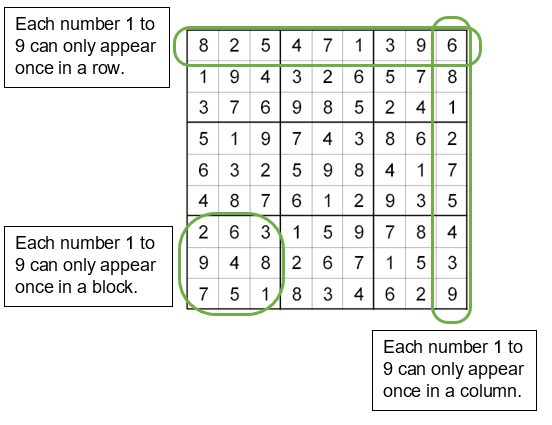
\includegraphics[width=0.5\paperwidth]{C:/Users/Admin/Desktop/Github/question_bank/LyX/static/img/9597-JPJC-2019-P1-Q4-1}
\par\end{center}

The puzzle can be displayed in this way on the computer. 
\noindent \begin{center}
\texttt{}%
\begin{tabular}{c}
\texttt{8 2 5 4 7 1 3 9 6}\tabularnewline
\texttt{1 9 4 3 2 6 5 7 8}\tabularnewline
\texttt{3 7 6 9 8 5 2 4 1}\tabularnewline
\texttt{5 1 9 7 4 3 8 6 2}\tabularnewline
\texttt{6 3 2 5 9 8 4 1 7}\tabularnewline
\texttt{4 8 7 6 1 2 9 3 5}\tabularnewline
\texttt{2 6 3 1 5 9 7 8 4}\tabularnewline
\texttt{9 4 8 2 6 7 1 5 3}\tabularnewline
\texttt{7 5 1 8 3 4 6 2 9}\tabularnewline
\end{tabular}
\par\end{center}

\noindent \begin{center}
\par\end{center}

\subsection*{Task 4.1 }

Write program code for a procedure \texttt{displayboard} that will
take a parameter \texttt{board} and display a puzzle declared as a
two-dimensional array. 

Copy and paste array \texttt{puzzle1} from the file \texttt{PUZZLES.txt}
into your program code. 

Call procedure \texttt{displayboard} to display \texttt{puzzle1}. 

\subsection*{Evidence 11: }
\begin{itemize}
\item Your program code for \texttt{displayboard} to display \texttt{puzzle1}. 
\item Screenshot of displaying \texttt{puzzle1} as a $9\times9$ Sudoku
puzzle.\hfill{} {[}5{]} 
\end{itemize}
To test the validity of a Sudoku puzzle, each of the rows, columns
and blocks can be checked to ensure that each number 1 to 9 only appears
once. 

\subsection*{Task 4.2 }

Write program code for a function \texttt{checkRow} that will check
all the nine rows of the puzzle to ensure that each number 1 to 9
only appears once. The function should take a parameter board and
return a Boolean value. 

\subsection*{Evidence 12: }

Your program code for \texttt{checkRow}.\hfill{} {[}6{]}

\subsection*{Task 4.3}

Write program code for a function \texttt{checkColumn} that will check
all the nine columns of the puzzle to ensure that each number 1 to
9 only appears once. The function should take a parameter \texttt{board}
and return a Boolean value.

\subsection*{Evidence 13: }

Your program code for \texttt{checkColumn}. \hfill{}{[}6{]}

\section*{Task 4.4 }

Write program code for a function \texttt{checkBlock} that will check
all the nine blocks of the puzzle to ensure that each number 1 to
9 only appear once. The function should take a parameter board and
return a Boolean value. 

\subsection*{Evidence 14: }

Your program code for \texttt{checkBlock}.\hfill{} {[}8{]}

\subsection*{Task 4.5 }

Write program code to call the three functions \texttt{checkrow},
\texttt{checkColumn}, and \texttt{checkBlock} to test the validity
of \texttt{puzzle1}, \texttt{puzzle2}, and \texttt{puzzle3} given
in the file \texttt{PUZZLES.txt}. Copy and paste these puzzles into
your program code. Your program should first display the puzzle before
printing statement(s) to show whether the puzzle is valid or not.
If invalid, state whether the invalidity is due to the row, column
or block.

\subsection*{Evidence 15:}

\textbullet{} Your program code for task 4.5 

\textbullet{} Screenshot of running task 4.5\hfill{} {[}5{]}

 \newpage 

\item \textbf{{[}JPJC/PRELIM/9597/2019/P2/Q1{]} }

Furniture retailer XFurniture is currently using a manual, paper-based
ordering system. 

The customer visits the show room and informs the salesperson his/her
furniture selection. After which, the salesperson asks the filing
clerk to locate the relevant paper files that contain all the necessary
details of the chosen item in the file cabinet. The files contain
the following information of a furniture item:
\begin{itemize}
\item item code 
\item description of item 
\item price of item 
\item delivery time 
\item details of the supplier
\end{itemize}
The customer pays for the purchase and the salesperson hands the original
purchase order, and a duplicate copy to the customer and the filing
clerk respectively. At the end of the day, the filing clerk will record
the total sales for the day and proceed to order the furniture from
the supplier by sending them a purchase order of the consolidated
furniture items sold for the day. 

The management of XFurniture decides to replace its current system
with a server--based ordering system. 

A system developer from an IT consultant firm is employed to carry
out the project. The first task is to write a project proposal. 
\begin{enumerate}
\item One section of the project proposal is the Problem Statement which
lists the problems in the current system. Write the Problem Statement.
\hfill{}{[}4{]}
\end{enumerate}
The system developer draws up a list of activities that will be required
for the completion of the software project:
\noindent \begin{center}
\begin{tabular}{|c|l|c|}
\hline 
Identifier & Activity & Estimated Duration (weeks)\tabularnewline
\hline 
A & Order and deliver the new database system and server & 4\tabularnewline
\hline 
B & Design and install the network infrastructure & 7\tabularnewline
\hline 
C & Order, deliver and install new PCs and printer & 9\tabularnewline
\hline 
D & est the database system, server and network & 3\tabularnewline
\hline 
E & Test the PCs with the server and network & 2\tabularnewline
\hline 
F & Copy existing sales data to the new database system & 1\tabularnewline
\hline 
G & Copy other existing PC software to the new PCs & 3\tabularnewline
\hline 
H & Test all software and database on the new PCs and server & 1\tabularnewline
\hline 
I & Train users & 2\tabularnewline
\hline 
\end{tabular}
\par\end{center}

Tasks A, B and C can be undertaken at the same time, but Task A and
Task B must be completed before Task D can commence. Tasks C and D
must be completed before Task E can begin. Task E must be completed
before Tasks F and G can start. Tasks F and G can be undertaken at
the same time, but both must be completed before Task H can commence.
Task I must follow Task H. 
\begin{enumerate}
\item[(b)]  Draw a PERT chart for this project. Provide a node key explaining
the layout and contents of the nodes used in your diagram. \hfill{}{[}4{]} 
\item[(c)]  Copy and complete the following table with the earliest and latest
start times, the earliest and latest finish times, duration, and float
time for each task. 
\noindent \begin{center}
\begin{tabular}{|c|c|c|c|c|c|c|}
\hline 
Task & EST & LST & EFT & LFT & Duration & Float\tabularnewline
\hline 
A & 0 & 3 & 4 & 7 & 4 & 3\tabularnewline
\hline 
B &  &  &  &  & 7 & \tabularnewline
\hline 
C &  &  &  &  & 9 & \tabularnewline
\hline 
D &  &  &  &  & 3 & \tabularnewline
\hline 
E &  &  &  &  & 2 & \tabularnewline
\hline 
F & 12 & 14 & 13 & 15 & 1 & \tabularnewline
\hline 
G &  &  &  &  & 3 & \tabularnewline
\hline 
H & 15 & 15 & 16 & 16 & 1 & \tabularnewline
\hline 
I & 16 & 16 & 18 & 18 & 2 & 0\tabularnewline
\hline 
\end{tabular} 
\par\end{center}

\hfill{}{[}4{]}
\item[(d)]  State the critical path.\hfill{} {[}1{]}
\item[(e)]  State the minimum time required for the project to be completed.
\hfill{} {[}1{]}
\item[(f)]  Dummy task may be used in PERT chart. What is a dummy task? \hfill{}
{[}1{]}
\item[(g)]  Draw a Gantt chart for the same project tasks, showing each of these
tasks, all dependencies, and the duration of each task. Highlight
the critical path on the Gantt chart.\hfill{} {[}4{]}
\end{enumerate}

 \newpage 

\item \textbf{{[}JPJC/PRELIM/9597/2019/P2/Q2{]} }

A project\textquoteright s software development life cycle includes
analysis, design, development, testing, implementation, and evaluation
stages.
\begin{enumerate}
\item Describe the following testing strategies that might be carried out
during a software development project, and explain how each type of
the testing strategy contributes to the overall quality of the project\textquoteright s
deliverables. 
\begin{enumerate}
\item Bottom-up testing. 
\item Top-down testing. \hfill{}{[}6{]}
\end{enumerate}
\item State two methods that could be used to implement a newly developed
system. Give a reason for each of the method chosen. \hfill{}{[}4{]}
\end{enumerate}
\item \textbf{{[}JPJC/PRELIM/9597/2019/P2/Q3{]} }
\begin{enumerate}
\item \textbf{Copy} and \textbf{complete} the algorithm for a binary search
written in pseudocode shown below. It is given that the data being
searched is stored in the array \texttt{SearchData{[}63{]}}, and the
item of data being searched is stored in the variable \texttt{SearchItem}. 

\noindent %
\noindent\begin{minipage}[t]{1\columnwidth}%
\texttt{X <- 0 }

\texttt{Low <- 1 }

\texttt{High <- \dots \dots \dots \dots \dots \dots \dots \dots \dots \dots \dots \dots \dots \dots \dots{} }

\texttt{WHILE (High >= Low) AND (\dots \dots \dots \dots \dots \dots \dots \dots \dots \dots \dots \dots \dots \dots \dots \dots \dots \dots \dots )}

\texttt{\qquad{}Middle INT((High + Low)/2) }

\texttt{\qquad{}IF SearchData{[}Middle{]} = SearchItem }

\texttt{\qquad{}\qquad{}THEN }

\texttt{\qquad{}\qquad{}\qquad{}X <- Middle }

\texttt{\qquad{}\qquad{}ELSE}

\texttt{\qquad{}\qquad{}\qquad{}IF SearchData{[}Middle{]} < SearchItem }

\texttt{\qquad{}\qquad{}\qquad{}\qquad{}THEN}

\texttt{\qquad{}\qquad{}\qquad{}\qquad{}\qquad{}Low <- Middle
+ 1}

\texttt{\qquad{}\qquad{}\qquad{}\qquad{}ELSE }

\texttt{\qquad{}\qquad{}\qquad{}\qquad{}\qquad{}IF SearchData{[}Middle{]}
> SearchItem }

\texttt{\qquad{}\qquad{}\qquad{}\qquad{}\qquad{}\qquad{}THEN}

\texttt{\qquad{}\qquad{}\qquad{}\qquad{}\qquad{}\qquad{}\qquad{}\dots \dots \dots \dots \dots \dots \dots \dots \dots \dots \dots \dots \dots \dots \dots \dots{} }

\texttt{\qquad{}\qquad{}\qquad{}\qquad{}\qquad{}ENDIF }

\texttt{\qquad{}\qquad{}\qquad{}ENDIF }

\texttt{\qquad{}ENDIF }

\texttt{ENDWHILE }%
\end{minipage}

\hfill{}{[}3{]}
\item State the maximum number of comparisons that are required to find
an item which is present in \texttt{SearchData}. \hfill{} {[}1{]}
\item You will change the binary search algorithm to a recursive algorithm
and write the equivalent program code in the form of a procedure.
Name the recursive procedure \texttt{BinarySearch}. Use the following
variables: 
\noindent \begin{center}
\begin{tabular}{|l|l|l|}
\hline 
\textbf{Variable} & \textbf{Data Type} & \textbf{Description}\tabularnewline
\hline 
\texttt{SearchData} & \texttt{ARRAY{[}63{]} : INTEGER} & global array\tabularnewline
\hline 
\texttt{SearchItem} & \texttt{INTEGER} & global variable\tabularnewline
\hline 
\texttt{X} & \texttt{INTEGER} & global variable\tabularnewline
\hline 
\texttt{Low} & \texttt{INTEGER} & parameter\tabularnewline
\hline 
\texttt{High} & \texttt{INTEGER} & global variable\tabularnewline
\hline 
\texttt{Middle} & \texttt{INTEGER} & local variable\tabularnewline
\hline 
\end{tabular} 
\par\end{center}

Write pseudocode or program code for the recursive procedure \texttt{BinarySearch}.
\hfill{}{[}4{]}
\end{enumerate}

 \newpage 

\item \textbf{{[}JPJC/PRELIM/9597/2019/P2/Q4{]} }

Object-oriented programming is used to store and process data for
a company\textquoteright s payroll. 
\begin{center}
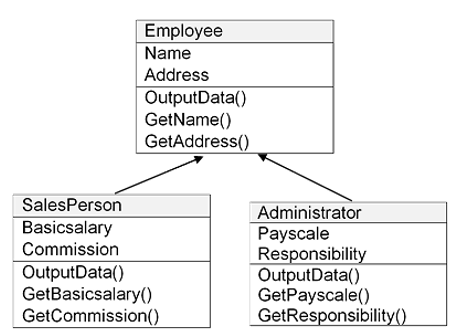
\includegraphics[width=0.5\paperwidth]{C:/Users/Admin/Desktop/Github/question_bank/LyX/static/img/9597-JPJC-2019-P2-Q4-1}
\par\end{center}
\begin{enumerate}
\item With reference to the class diagram shown above, explain: 
\begin{enumerate}
\item data encapsulation, and how classes support information hiding and
implementation independence. \hfill{}{[}3{]}
\item inheritance, and how it promotes software reusability. \hfill{}{[}2{]}
\end{enumerate}
\end{enumerate}

 \newpage 

\item \textbf{{[}JPJC/PRELIM/9597/2019/P2/Q5{]} }

With reference to \textbf{Question 1}, a server--based ordering system
will be implemented in XFurniture.

Local Area Network (LAN) will be used for the staff and customers.
\begin{enumerate}
\item Explain the meaning of a protocol for communication within the LAN.
\hfill{}{[}1{]}
\item State the purposes of switches and routers in a network. \hfill{}{[}4{]}
\item Explain the differences between using packet switching and circuit
switching in the transmission of a message. \hfill{} {[}3{]}
\item The LAN is connected to the Internet. Discuss the social and ethical
effects of allowing staff to have unrestricted access to the Internet.
\hfill{}{[}4{]}
\item Customers are now able to order furniture online after logging in
to the XFurniture online system. 
\begin{enumerate}
\item Explain why authentication techniques are necessary. \hfill{} {[}2{]}
\item Explain \textbf{two} methods for ensuring security of a network application.
\hfill{}{[}2{]}
\item A security policy is a formalised statement that defines how security
will be implemented within XFurniture. Explain why staff members are
required to know the need for privacy and integrity of data. \hfill{}{[}2{]}
\end{enumerate}
\item Explain why XFurniture has chosen to implement their server--based
ordering system over the intranet. \hfill{}{[}4{]}
\item An alternative to a server--based ordering system is to subscribe
the services of cloud computing. State the \textbf{three} services
provided by cloud computing, and explain how they can benefit XFurniture.
\hfill{} {[}6{]}
\end{enumerate}

 \newpage 

\item \textbf{{[}JPJC/PRELIM/9597/2019/P2/Q6{]} }

A reservation form used for booking JP Hotel rooms is shown:
\begin{center}
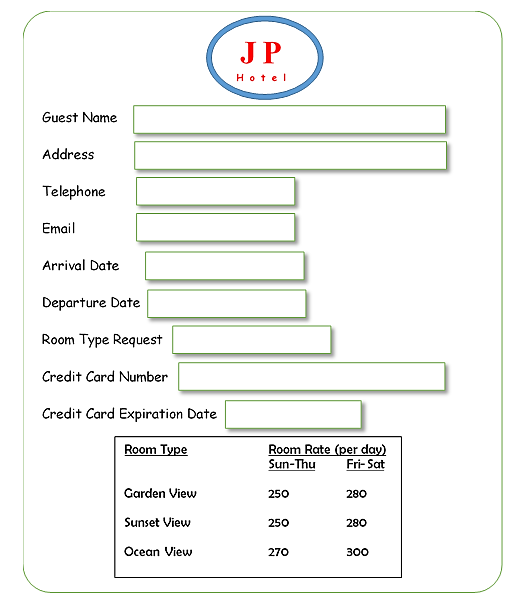
\includegraphics[width=0.5\paperwidth]{C:/Users/Admin/Desktop/Github/question_bank/LyX/static/img/9597-JPJC-2019-P2-Q6-1}
\par\end{center}

There are three room types available and the room rates are higher
for arrival on Fridays and Saturdays. A normalised database solution
is designed to store data for the hotel using a number of tables.
\begin{enumerate}
\item Draw an E-R diagram that shows these tables and the relationships
between them. \hfill{}{[}4{]}
\item Using standard notation, write the table descriptions of the tables
in part \textbf{(a)}. \hfill{} {[}6{]}
\end{enumerate}
To book a room in JP Hotel, the guest can fill in the hotel reservation
form with details specified on the form. After the form is submitted,
the credit card number and its expiration date are validated. The
guest will be notified with a message if the credit card number is
invalid. If the credit card number is valid, details of the guests
will be stored in a file. The room type requested by the guest will
then be checked for availability. If room type requested by guest
is available, a confirmation letter will be sent to the guest. 
\begin{enumerate}
\item[(c)]  Draw a data flow diagram for the hotel reservation system. \hfill{}{[}8{]}
\item[(d)]  A hotel room accommodates two guests and also includes breakfast
for two. The hotel allows for an additional guest to stay in a room
booked for two guests at a charge of \$80. An extra bed may be requested
for the additional guest at a charge of \$20. Breakfast can also be
provided for the additional guest at \$20.
\begin{enumerate}
\item Create a decision table showing all the possible conditions and actions.
\hfill{} {[}4{]}
\item Simplify your decision table by removing redundancies. \hfill{} {[}2{]}
\end{enumerate}
\end{enumerate}

 \newpage 

\item \textbf{{[}JPJC/PRELIM/9597/2019/P2/Q7{]} }
\begin{enumerate}
\item Computers use character codes that can be represented by ASCII and
Unicode. Explain the differences between these two character encoding
systems. \hfill{}{[}2{]}
\item Given that \textbf{two} bytes are used to represent a positive integer,
what is the denary number that corresponds to the \textbf{two} successive
bytes below? 
\noindent \begin{center}
\texttt{10010101 00110011} 
\par\end{center}

\noindent \begin{center}
\hfill{}\texttt{ }{[}2{]}
\par\end{center}
\item What is the hexadecimal number of the \textbf{two} bytes in \textbf{(b)}?
\hfill{} {[}2{]}
\end{enumerate}

 \newpage 

\item \textbf{{[}JPJC/PRELIM/9597/2019/P2/Q8{]} }

An Abstract Data Type (ADT) is a type (or class) for objects whose
behavior is defined by a set of value and a set of operations. 

A linked list ADT has the following operations defined:
\begin{enumerate}
\item[i. ]  \texttt{Create(x)} -- creates an empty linked list \texttt{x}.
\item[ii.]  \texttt{Insert(x,item,i)} -- inserts new value, \texttt{item},
into linked list \texttt{x} so that it is at position \texttt{i} in
the linked list.
\item[iii.]  \texttt{Delete(x,i)} -- deletes the \texttt{item} at position \texttt{i}
in the linked list \texttt{x}.
\item[iv.]  \texttt{Read(x,i)} -- returns the \texttt{item} at position \texttt{i}
in the linked list \texttt{x}.
\item[v.]  \texttt{Length(x)} -- returns the number of items in the linked
list \texttt{x}.
\item[vi.]  \texttt{IsEmptyList(x)} -- returns true if linked list \texttt{x}
is empty.
\end{enumerate}
The linked list is implemented by the use of a collection of nodes
that has \textbf{two} parts: the \textbf{data} and a \textbf{pointer
to the next item} in the linked list. In addition, there is a Start
pointer which points to the first node in the list. 
\begin{enumerate}
\item Assume a node with the following structure: 
\begin{center}
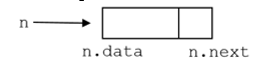
\includegraphics[width=0.25\paperwidth]{C:/Users/Admin/Desktop/Github/question_bank/LyX/static/img/9597-JPJC-2019-P2-Q8-1}
\par\end{center}

Complete the algorithm to implement the 'Delete' operation: \hfill{}{[}5{]}

\noindent %
\noindent\begin{minipage}[t]{1\columnwidth}%
\texttt{PROCEDURE Delete (x, i) }

\texttt{\qquad{}IF Length(x) = 0 THEN }

\texttt{\qquad{}\qquad{}....................................A.................................... }

\texttt{\qquad{}ENDIF }

\texttt{\qquad{}IF i = 1 THEN // situation 1: delete the 1st node }

\texttt{\qquad{}\qquad{}temp <- Start }

\texttt{\qquad{}\qquad{}....................................B.................................... }

\texttt{\qquad{}ELSE // situation 2 : delete middle node }

\texttt{\qquad{}\qquad{}Previous <- NULL }

\texttt{\qquad{}\qquad{}Current <- Start }

\texttt{\qquad{}\qquad{}FOR n <- 1 TO (i \textendash{} 1) STEP 1 }

\texttt{\qquad{}\qquad{}\qquad{}....................................C.................................... }

\texttt{\qquad{}\qquad{}\qquad{}....................................D.................................... }

\texttt{\qquad{}\qquad{}NEXT n }

\texttt{\qquad{}\qquad{}\qquad{}....................................E.................................... //
make the deletion }

\texttt{\qquad{}ENDIF }

\texttt{ENDPROCEDURE }%
\end{minipage}
\item Show how the following operations for an ADT called QUEUE using the
linked list ADT operations can be implemented. 
\begin{enumerate}
\item Create new queue. \hfill{}{[}1{]}
\item Add item to a queue. \hfill{}{[}2{]}
\item Delete item from a queue. \hfill{} {[}2{]}
\end{enumerate}
\end{enumerate}

 \newpage 

\item \textbf{{[}JPJC/PRELIM/9597/2019/P2/Q9{]} }

A binary search tree is stored as an array of records. Each record
represents a node and consists of the data and a left pointer and
a right pointer. After a number of records are inserted, the tree
is as shown. 

The array is called \texttt{BinaryTree}. 

The notation \texttt{BinaryTree{[}Root{]}.Data} will access the data
at root node.
\noindent \begin{center}
\begin{tabular}{c|c|c|c|}
\multicolumn{4}{c}{\texttt{BinaryTree}}\tabularnewline
\cline{2-4} \cline{3-4} \cline{4-4} 
 & \texttt{LeftPtr} & \texttt{DataValue} & \texttt{RightPtr}\tabularnewline
\cline{2-4} \cline{3-4} \cline{4-4} 
\texttt{{[}1{]}} & \texttt{2} & \texttt{Jay} & \texttt{3}\tabularnewline
\cline{2-4} \cline{3-4} \cline{4-4} 
\texttt{{[}2{]}} & \texttt{4} & \texttt{Gel} & \texttt{0}\tabularnewline
\cline{2-4} \cline{3-4} \cline{4-4} 
\texttt{{[}3{]}} & \texttt{0} & \texttt{Ken} & \texttt{5}\tabularnewline
\cline{2-4} \cline{3-4} \cline{4-4} 
\texttt{{[}4{]}} & \texttt{0} & \texttt{Ace} & \texttt{0}\tabularnewline
\cline{2-4} \cline{3-4} \cline{4-4} 
\texttt{{[}5{]}} & \texttt{6} & \texttt{Pan} & \texttt{0}\tabularnewline
\cline{2-4} \cline{3-4} \cline{4-4} 
\texttt{{[}6{]}} & \texttt{0} & \texttt{Max} & \texttt{0}\tabularnewline
\cline{2-4} \cline{3-4} \cline{4-4} 
\texttt{{[}7{]}} & \texttt{8} &  & \tabularnewline
\cline{2-4} \cline{3-4} \cline{4-4} 
\texttt{{[}8{]}} & \texttt{9} &  & \tabularnewline
\cline{2-4} \cline{3-4} \cline{4-4} 
\texttt{{[}9{]}} & \texttt{0} &  & \tabularnewline
\cline{2-4} \cline{3-4} \cline{4-4} 
\end{tabular}
\par\end{center}

\noindent \begin{center}
\texttt{}%
\begin{tabular}{c|c|c|c|}
\cline{2-2} \cline{4-4} 
\texttt{Root} & \texttt{1} & \texttt{NextFree} & \texttt{7}\tabularnewline
\cline{2-2} \cline{4-4} 
\end{tabular}\texttt{ }
\par\end{center}
\begin{enumerate}
\item Draw the binary search tree. \hfill{}{[}2{]}
\item Complete the algorithm to find a node in a binary search tree. This
function will return a pointer to node.\hfill{} {[}4{]}

\noindent %
\noindent\begin{minipage}[t]{1\columnwidth}%
\texttt{FUNCTION FindNode(SearchItem) RETURNS INTEGER }

\texttt{\qquad{}TempPtr <- Root }

\texttt{\qquad{}WHILE TempPtr <> NULL AND ............A............}

\texttt{\qquad{}\qquad{}IF ............B............ THEN }

\texttt{\qquad{}\qquad{}\qquad{}TempPtr <- BinaryTree{[}TempPtr{]}.LeftPtr }

\texttt{\qquad{}\qquad{}ELSE }

\texttt{\qquad{}\qquad{}\qquad{}............C............ }

\texttt{\qquad{}\qquad{}ENDIF }

\texttt{\qquad{}ENDWHILE }

\texttt{\qquad{}............D............}

\texttt{ENDFUNCTION} %
\end{minipage}
\item Write an algorithm for a pre-order traversal of the binary search
tree. \hfill{}{[}4{]}
\end{enumerate}

 \newpage 

\item \textbf{{[}NYJC/PRELIM/9597/2019/P1/Q1{]} }

The number of rainy days for each year and month is stored in the
file \texttt{RAINFALL.txt}. The first line of the file contains the
heading description for the data. Each line of data is stored in the
format \texttt{YYYY-MM,99} where \texttt{YYYY} is the year, \texttt{MM}
is the month and \texttt{99} is the number of days. Thus '\texttt{1982-
01,10}' means there were 10 rainy days in the month of January, 1982. 

You are required to write a program to: 
\begin{itemize}
\item Read the data in the file. 
\item Calculate the total number of rainy days for each year by adding all
the months\textquoteright{} rainy days for that year. 
\item Create a new file \texttt{RAINFALLYEAR.txt}. 
\item Write the heading description in the first line as \textquotedbl Year,Rainy
Days\textquotedblright . 
\item For each subsequent line, write to the file in the format \texttt{YYYY,999}
where \texttt{YYYY} is the year and \texttt{999} is the total number
of rainy days (up to 3 digits) for that year. 
\end{itemize}

\subsection*{Task 1.1 }

Write program code for this task. 

\subsection*{Evidence 1: }

Your program code. \hfill{}{[}8{]}

\subsection*{Task 1.2 }

Write program code for a procedure \texttt{ShowMenu} to display the
following menu: 
\begin{enumerate}
\item[1.] \texttt{ Query total rainy days in any year}
\item[2.] \texttt{ Query by year the month of highest rainy days }
\item[3.] \texttt{ -1 to Exit}
\end{enumerate}

\subsection*{Evidence 2: }

Your program code.\hfill{} {[}2{]}

\subsection*{Task 1.3 }

Implement a program that displays \texttt{ShowMenu} and asks the user
for their choice. Create functions \texttt{Query1} and \texttt{Query2}
which corresponds to the menu selection option \texttt{1} and \texttt{2}
respectively. When option \texttt{1} is selected, \texttt{Query1}
should run and ask the user to input the year. \texttt{Query1} will
return the total number of rainy days or a suitable message if data
for that year is not available. 

When option \texttt{2} is selected, \texttt{Query2} should execute
and ask the user for the year. \texttt{Query2} will return the month
with the highest number of rainy days in that year in words (e.g.
January, August, or December) or a suitable message if data for that
year is not available. 

For both \texttt{Query1} and \texttt{Query2}, appropriate validation
of the user input for year should be done. The program will display
\texttt{ShowMenu} after each valid query until option \texttt{3} is
selected.

\subsection*{Evidence 3: }

Your program code. \hfill{}{[}8{]}

\subsection*{Task 1.4 }

Design 3 test data which tests the functionality of your program. 

\subsection*{Evidence 4: }

A screenshot for each test case you considered. Annotate the screenshot
explaining the purpose of each test. \hfill{}{[}3{]}

 \newpage 

\item \textbf{{[}NYJC/PRELIM/9597/2019/P1/Q2{]} }

The following is the algorithm for a recursive insertion sort on an
array of size $n$. 
\begin{enumerate}
\item[1.]  Base Case: If array size is 1 or smaller, return. 
\item[2.]  Recursively sort first n -- 1 elements. 
\item[3.]  Insert last element at its correct position in sorted array. 
\end{enumerate}

\subsection*{Task 2.1 }

Write program code for this algorithm to implement a recursive insertion
sort function. Use the sample array data available from text file
\texttt{COUNTRIES.txt} and paste this into your programming code.
Your program should display the sorted items with each item shown
per line. 

\subsection*{Evidence 5: }

Your program code. \hfill{}{[}8{]}

\subsection*{Task 2.2 }

Amend your code to display the insertion process done during each
recursive call. Each recursive call should display a line as follows: 

\texttt{Element at position n is being inserted in position j }

Replace \texttt{n} and \texttt{j} to show the actual index value. 

\subsection*{Evidence 6: }

Your amended program code. \hfill{}{[}3{]}

\subsection*{Evidence 7:}

One screenshot of the output. \hfill{} {[}2{]}

 \newpage 

\item \textbf{{[}NYJC/PRELIM/9597/2019/P1/Q3{]} }

Create a binary tree Abstract Data Type (ADT) with commands to create
a new tree, insert data items to the tree and print the tree. 

The sequence of commands 
\noindent \begin{center}
\begin{tabular}{l}
Create a new tree\tabularnewline
Add to tree (15) \tabularnewline
Add to tree (10) \tabularnewline
Add to tree (20) \tabularnewline
Add to tree (8) \tabularnewline
Add to tree (12) \tabularnewline
Add to tree (18) \tabularnewline
Add to tree (25)\tabularnewline
\end{tabular}
\par\end{center}

would create the following binary tree: 
\begin{center}
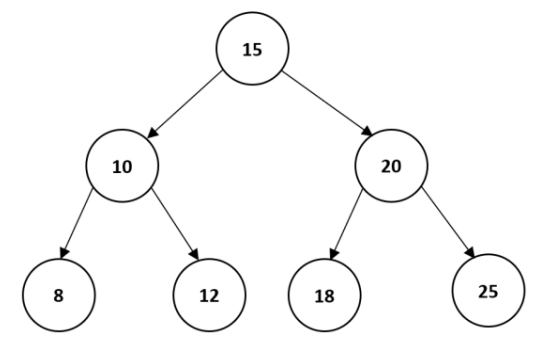
\includegraphics[width=0.25\paperwidth]{C:/Users/Admin/Desktop/Github/question_bank/LyX/static/img/9597-NYJC-2019-P1-Q3-1}
\par\end{center}

The program to implement this ADT will use the classes Tree and Node
designed as follows: 
\begin{center}
\begin{tabular}{|l|}
\hline 
\texttt{ToDo}\tabularnewline
\hline 
\texttt{root : Node}\tabularnewline
\hline 
\texttt{constructor()}\tabularnewline
\texttt{add(newItem)}\tabularnewline
\texttt{printTreeInOrder()}\tabularnewline
\hline 
\end{tabular}%
\begin{tabular}{|l|}
\hline 
\texttt{Node}\tabularnewline
\hline 
\texttt{key : INTEGER}\tabularnewline
\texttt{left : Node}\tabularnewline
\texttt{right : Node}\tabularnewline
\hline 
\texttt{constructor()}\tabularnewline
\texttt{insert(key : INTEGER)}\tabularnewline
\hline 
\end{tabular}
\par\end{center}

\subsection*{Task 3.1 }

Write program code to define the classes \texttt{Tree} and \texttt{Node}.

\subsection*{Evidence 8: }

Your program code. \hfill{}{[}16{]}

\subsection*{Task 3.2 }
\begin{itemize}
\item Write program code for a procedure \texttt{CreateTreefromArray} that
accepts an array of unsorted unique integers passed in via a parameter. 
\item The procedure will read each integer in the array and construct a
binary tree using your classes \texttt{Tree} and \texttt{Node}. 
\item Call \texttt{printTreeInOrder} to display the output (numbers shown
will always be sorted). 
\item Test your program by copying the input data found in \texttt{BST.txt}
into your code. 
\end{itemize}

\subsection*{Evidence 9: }

Your \texttt{CreateTreefromArray} program code. \hfill{}{[}4{]}

\subsection*{Evidence 10: }

A screenshot of the output. \hfill{}{[}2{]}

\subsection*{Task 3.3}

A binary tree created from keys that are in ascending order will result
in an unbalanced binary tree.

For instance, the sequence of commands
\noindent \begin{center}
\begin{tabular}{l}
Create a new tree \tabularnewline
Add to tree (8) \tabularnewline
Add to tree (10) \tabularnewline
Add to tree (12) \tabularnewline
Add to tree (15)\tabularnewline
Add to tree (18) \tabularnewline
Add to tree (20)\tabularnewline
Add to tree (25)\tabularnewline
\end{tabular}
\par\end{center}

will result in a tree that looks as follows: 
\begin{center}
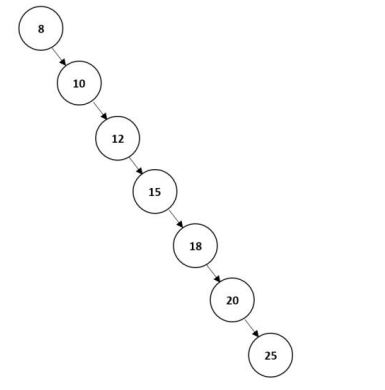
\includegraphics[width=0.25\paperwidth]{C:/Users/Admin/Desktop/Github/question_bank/LyX/static/img/9597-NYJC-2019-P1-Q3-2}
\par\end{center}

Amend procedure \texttt{CreateTreefromArray} so that the created tree
from any input array of integers will be balanced where the number
of items on the left and right subtree will roughly be divided equally
(Hint: input array must first be sorted).

\subsection*{Evidence 11: }

Your amended program code. \hfill{}{[}6{]}

\subsection*{Task 3.4 }

Create a function \texttt{FindKthSmallest} that returns the $k$th
smallest element in your binary tree. If $k=5$ the $k$th smallest
element will be 18. Your function should not need to use extra space
(e.g. creating a new array) to solve the problem other than using
a temp variable(s). 

\subsection*{Evidence 12: }

Your program code for \texttt{FindKthSmallest}. \hfill{}{[}4{]}

\subsection*{Evidence 13:}

Produce a screenshot showing the retrieval of the 5th smallest element
from the tree created earlier. \hfill{}{[}2{]}

 \newpage 

\item \textbf{{[}NYJC/PRELIM/9597/2019/P1/Q4{]} }

To encrypt a message, a keyword cipher is used. It is a form of monoalphabetic
substitution where a keyword is used as the key. The key is used to
determine the letter matchings of the cipher alphabet to the plain
alphabet. Repeating letters in the key is removed. For instance, if
the key used is \texttt{'SECRET'}, the cipher alphabet generated will
be as follows: 

\begin{tabular}{lcccccccccccccccccccccccccc}
Plain text: & \texttt{A} & \texttt{B} & \texttt{C} & \texttt{D} & \texttt{E} & \texttt{F} & \texttt{G} & \texttt{H} & \texttt{I} & \texttt{J} & \texttt{K} & \texttt{L} & \texttt{M} & \texttt{N} & \texttt{O} & \texttt{P} & \texttt{Q} & \texttt{R} & \texttt{S} & \texttt{T} & \texttt{U} & \texttt{V} & \texttt{W} & \texttt{X} & \texttt{Y} & \texttt{Z}\tabularnewline
Cipher Alphabet: & \texttt{S} & \texttt{E} & \texttt{C} & \texttt{R} & \texttt{T} & \texttt{A} & \texttt{B} & \texttt{D} & \texttt{F} & \texttt{G} & \texttt{H} & \texttt{I} & \texttt{J} & \texttt{K} & \texttt{L} & \texttt{M} & \texttt{N} & \texttt{O} & \texttt{P} & \texttt{Q} & \texttt{U} & \texttt{V} & \texttt{W} & \texttt{X} & \texttt{Y} & \texttt{Z}\tabularnewline
\end{tabular}

After the key\textquoteright s unique letters is used up, the rest
of the ciphertext letters are used in alphabetical order, excluding
those already used in the key. Thus, to encode the word \textquoteleft \texttt{Attack}\textquoteright ,
\textquoteleft \texttt{A}\textquoteright{} is replaced with \texttt{'S'},
\texttt{'t'} is replaced with \texttt{'Q'}, and so on giving the encrypted
word as \texttt{'SQQSCH'}. 

\subsection*{Task 4.1 }

Write program code for a function to generate an array of the cipher
alphabet given a key. 
\noindent \begin{center}
\texttt{FUNCTION Cipher (NewAlphabet : ARRAY, Key : STRING) }
\par\end{center}

The function has two parameters and returns the \texttt{NewAlphabet}
array with the correct cipher alphabet based on the \texttt{Key} parameter. 

\subsection*{Evidence 14:}

Your program code. \hfill{} {[}6{]}

\subsection*{Task 4.2 }

Write driver code that asks the user to enter a key that contains
only letters, calls function Cipher and displays the cipher alphabet
(all in uppercase) in one line. Do appropriate data validation on
the input key. 

\subsection*{Evidence 15: }

Your program code. \hfill{} {[}3{]}

\subsection*{Task 4.3 }

Design three suitable test cases and provide screenshot evidence for
your testing. 

\subsection*{Evidence 16: }

Annotated screenshots for each test data run. \hfill{} {[}3{]}

\subsection*{Task 4.4 }

Develop your program further to display the following menu: 
\begin{enumerate}
\item[1.]  Encode a message
\item[2.]  Decode a message 
\item[3.]  -1 to Quit
\end{enumerate}
Implement the menu options to allow a line of text to be encoded or
decoded. For each option, ask for the cipher key and the message that
is to be encoded or decoded. Test your program with the key \texttt{'TOPSECRET'}
and the message \texttt{'I will score A for Computing}'. 

\subsection*{Evidence 17: }

Your program code. \hfill{}{[}10{]}

\subsection*{Evidence 18: }

Screenshot(s) showing your output. \hfill{}{[}2{]}

\subsection*{Task 4.5 }

Frequency analysis is a common method used by code breakers to break
monoalphabetic substitution ciphers. The first step is to analyse
the coded message and construct a frequency table of all the letters
appearing in the coded message. 

Write a program that reads the content from the file \texttt{INTERCEPT.txt}.
The text in this file contains a coded message. Construct a frequency
table (ignore punctuation marks) as follows using a suitable data
structure: 

\begin{tabular}{lcccccccccccccccccccccccccc}
Ciphertext Letter: & \texttt{A} & \texttt{B} & \texttt{C} & \texttt{D} & \texttt{E} & \texttt{F} & \texttt{G} & \texttt{H} & \texttt{I} & \texttt{J} & \texttt{K} & \texttt{L} & \texttt{M} & \texttt{N} & \texttt{O} & \texttt{P} & \texttt{Q} & \texttt{R} & \texttt{S} & \texttt{T} & \texttt{U} & \texttt{V} & \texttt{W} & \texttt{X} & \texttt{Y} & \texttt{Z}\tabularnewline
Frequency: & \texttt{5} & \texttt{2} & $\cdots$ &  &  &  &  &  &  &  &  &  &  &  &  &  &  &  &  &  &  &  &  &  &  & \tabularnewline
\end{tabular}

Your program will then display the table sorted by descending order
showing the most used letter and its frequency first followed by the
next highest and so on.

Partial sample output: 

\begin{tabular}{lcccc}
Ciphertext Letter: & \texttt{S} & \texttt{O} & \texttt{G} & \texttt{$\cdots$}\tabularnewline
Frequency: & \texttt{88} & \texttt{85} & \texttt{67} & $\cdots$\tabularnewline
\end{tabular}

\subsection*{Evidence 19: }

Your program code. \hfill{} {[}7{]}

\subsection*{Evidence 20: }

Screenshot of output. \hfill{}{[}1{]}

 \newpage 

\item \textbf{{[}NYJC/PRELIM/9597/2019/P2/Q1{]} }
\begin{enumerate}
\item Database management systems are aimed at solving a number of problems
associated with traditional file-based systems. Describe three such
problems and explain how they are solved by database management systems.
\hfill{} {[}6{]}
\item A national car hire company uses a relational database. Cars are available
for hire from a large number of depots around the country. Two entities
(or records) are CARS-FOR-HIRE and DEPOTS.
\begin{enumerate}
\item Suggest four attributes (or fields) associated with the entity CARS-FOR-HIRE.
\hfill{}{[}4{]}
\item Draw a diagram showing the relationship between the entities CARS-FOR-HIRE
and DEPOTS. \hfill{}{[}1{]}
\item State one other entity which is related to either or both of the original
entities. Describe the relationship(s). Suggest an attribute for this
entity. \hfill{}{[}4{]}
\end{enumerate}
\end{enumerate}

 \newpage 

\item \textbf{{[}NYJC/PRELIM/9597/2019/P2/Q2{]} }

A stack is to be implemented using an array of 20 elements. 
\begin{enumerate}
\item Describe an algorithm to remove an item from a stack and place it
in a variable \texttt{x}. \hfill{}{[}4{]}
\item With the aid of examples, explain what nested functions or nested
subroutines are. \hfill{} {[}3{]}
\item Explain with the aid of diagrams or otherwise, how a stack can be
used by the operating system to process \textquotedblleft nested functions\textquotedblright{}
or \textquotedblleft nested subroutines\textquotedblright . \hfill{}{[}5{]}
\item Outline the data attributes and member functions for a class stack
abstract data type. You need not go into details as to how they will
be implemented. \hfill{}{[}6{]}
\end{enumerate}

 \newpage 

\item \textbf{{[}NYJC/PRELIM/9597/2019/P2/Q3{]} }

A large national electrical appliances company maintains an extensive
inventory of appliances for sale in a country. The company has twelve
specialised retail stores targeting the needs of different market
segments. Six of these stores are housed in a large mall in the capital,
but the other six are in different cities in the country. 

The six stores in the capital are linked using a LAN, while the other
six are linked via a WAN. 
\begin{enumerate}
\item Explain the difference between a LAN and a WAN. \hfill{} {[}2{]}
\item Wireless technology has become more popular in recent years. Describe
two reasons why the company will not replace its LAN network with
a wireless one. \hfill{} {[}4{]}
\item Discuss two security threats faced by the company\textquoteright s
LAN and measures that can be put in place to reduce these threats.
\hfill{} {[}6{]}
\end{enumerate}
The company is thinking of allowing all its sales personnel access
to this inventory. It can store this data on an intranet or cloud
storage. Discuss the relative merits and demerits of these two options.
\hfill{}{[}6{]}

 \newpage 

\item \textbf{{[}NYJC/PRELIM/9597/2019/P2/Q4{]} }

A company has decided to offer an in-house credit system by issuing
privileged customers an in-house credit-card which allows customers
to charge their purchases from the stores to the card, up to the customers\textquoteright{}
credit limits.
\begin{enumerate}
\item During a sales promotion, the store offers a discount of 15\% if a
customer\textquoteright s total purchase is greater or equal to \$200
but less than \$500. A discount of 20\% is given if the customer\textquoteright s
total purchase is greater or equal to \$500. For customers who had
exceeded their credit limits, the supervisor\textquoteright s approval
is required. Create a decision table or tree to represent the above
conditions and actions. \hfill{}{[}5{]}
\item In order to protect the privacy of data, many countries have passed
legislation to address this issue. Describe any 3 features of the
Personal Data Protection Act in Singapore that aims to do this. \hfill{}{[}6{]}
\end{enumerate}

 \newpage 

\item \textbf{{[}NYJC/PRELIM/9597/2019/P2/Q5{]} }

When a customer orders goods over the phone, the cashier will record
the order in an order form containing the items ordered and quantity,
customer address, delivery date and time and the amount payable. A
copy of this form will be given to the storeman who will pick the
goods and generate a delivery order (DO). The DO will be given to
the delivery man who will deliver the goods. The customer on collecting
the goods will sign on the DO and return a signed copy to the delivery
man. On his return, the delivery man will give the DO to the accounts
department who will generate an invoice. Invoices are kept in a file
until the next day where they will be mailed to the customers.
\begin{enumerate}
\item Draw a data flow diagram of the above processes.\hfill{} {[}8{]} 
\item Goods in the warehouse are divided into 2 main categories -- Kitchen
appliances (e.g. kettle, toasters and ovens) and Entertainment products
(e.g. LCD television, mp3 players and gaming consoles). Each item
has an item name, description, unit price and quantity on hand. Kitchen
appliances have an item weight, packing volume and colour. Entertainment
products have a serial number, country of manufacture and recommended
retail price.
\begin{enumerate}
\item Draw a class diagram of the above showing inheritance, their private
attributes and public methods.\hfill{} {[}6{]}
\item What is the purpose of a public method?\hfill{} {[}1{]}
\item What is the difference between a class and an object?\hfill{} {[}2{]}
\end{enumerate}
\item In relation to the diagram in part (b), explain the terms: 
\begin{enumerate}
\item Encapsulation; \hfill{}{[}2{]}
\item Inheritance;\hfill{} {[}2{]}
\item Data hiding; \hfill{}{[}2{]}
\item Polymorphism. \hfill{}{[}2{]}
\end{enumerate}
\end{enumerate}

 \newpage 

\item \textbf{{[}NYJC/PRELIM/9597/2019/P2/Q6{]} }

A linked list ADT with the following incomplete specification is given
as follows:
\begin{center}
\begin{tabular}{|l|}
\hline 
\texttt{LList}\tabularnewline
\hline 
\texttt{head : Node}\tabularnewline
\hline 
\texttt{constructor()}\tabularnewline
\texttt{addNode(s : Node)}\tabularnewline
\texttt{findmiddle(l : llist)-> INTEGER}\tabularnewline
\hline 
\end{tabular}%
\begin{tabular}{|l|}
\hline 
Node\tabularnewline
\hline 
\texttt{data : INTEGER}\tabularnewline
\texttt{nextPtr : Node}\tabularnewline
\hline 
\texttt{constructor()}\tabularnewline
\texttt{setData(s : INTEGER)}\tabularnewline
\texttt{setnextPtr(x : Node)}\tabularnewline
\texttt{getData(): INTEGER }\tabularnewline
\hline 
\end{tabular}
\par\end{center}
\begin{enumerate}
\item Explain the main difference between an array and a linked list data
structure.\hfill{} {[}2{]}
\item Using pseudo code, write an algorithm to implement \texttt{findmiddle}
that will return the data in the middle of the linked list in one
pass. \hfill{}{[}7{]}
\item State two applications of a linked list. \hfill{}{[}2{]}
\item State two other common methods (including parameters) that should
be included in the \texttt{LList} specification.\hfill{} {[}2{]}
\end{enumerate}

 \newpage 

\item \textbf{{[}RVHS/PRELIM/9597/2019/P1/Q1{]} }

\textbf{CID3 Team Grouping} 

In this question, you will help the CID3 students in forming CID3
groups for their projects. 

In \textquotedblleft \texttt{student\_cid.txt}\textquotedblright{} 

There are three fields on each line which indicates \texttt{name},
\texttt{role} and \texttt{gender} of 50 cid3 students. The fields
are separated by \textquoteleft ;\textquoteright{} 

\noindent %
\noindent\begin{minipage}[t]{1\columnwidth}%
\texttt{Rufus Schuck;Coder;F }

\texttt{Ione Wolfe;Dealer;F }

\texttt{Hillary Curl;Coder;M }

\texttt{\dots{} }%
\end{minipage}

\subsection*{Task 1.1 }

Implement the function \texttt{read\_data(filename)} which takes \texttt{filename}
as a string and returns a 2-dimension list that follows the format
as shown in the example below.

\noindent %
\noindent\begin{minipage}[t]{1\columnwidth}%
\texttt{>\textcompwordmark >\textcompwordmark > read\_data(\textquotedbl student\_cid.txt\textquotedbl ) }

\texttt{{[}{[}'Rufus Schuck', 'Coder', 'F'{]}, {[}'Ione Wolfe', 'Dealer',
'F'{]}, {[}'Hillary Curl', 'Coder', 'M'{]},\dots {]} }%
\end{minipage}

\subsection*{Evidence 1 }

Program code of function \texttt{read\_data}. \hfill{}{[}2{]}

\subsection*{Task 1.2}

Implement the function \texttt{gender\_count(cid\_student\_lst, is\_female)}
which takes a list \texttt{cid\_student\_lst} and a boolean \texttt{is\_female}
as inputs and returns the number of female students in \texttt{cid\_student\_lst}
if \texttt{is\_female} is \texttt{True}, otherwise return the number
of male students. \texttt{cid\_student\_lst} is the list obtained
in \textbf{Task 1.1}. 

\subsection*{Evidence 2 }

Program code of function \texttt{gender\_count}.\hfill{} {[}2{]}

\subsection*{Evidence 3 }

Screenshot of the output of the following: 

\noindent %
\noindent\begin{minipage}[t]{1\columnwidth}%
\texttt{cid\_student\_lst = read\_data(\textquotedbl student\_cid.txt\textquotedbl ) }

\texttt{print(gender\_count(cid\_student\_lst, True)) }

\texttt{print(gender\_count(cid\_student\_lst, False))}\hfill{}\texttt{
}{[}1{]}%
\end{minipage}

\subsection*{Task 1.3 }

Implement the procedure \texttt{role\_statistics(cid\_student\_lst)}
which takes a list \texttt{cid\_student\_lst} as input and output
the number of students for each role in the following format. (There
are more than 5 types of roles.) 

For example: 

\noindent %
\noindent\begin{minipage}[t]{1\columnwidth}%
\texttt{>\textcompwordmark >\textcompwordmark > cid\_student\_lst
= read\_data(\textquotedbl student\_cid.txt\textquotedbl ) }

\texttt{>\textcompwordmark >\textcompwordmark > role\_statistics(cid\_student\_lst) }

\texttt{Role ~~~~~~~Number }

\texttt{Coder ~~~~~~11 }

\texttt{Dealer ~~~~~13 }

\texttt{Designer ~~~14 }

\texttt{Empathizer ~14 }

\texttt{Maker ~~~~~~12 }%
\end{minipage}

Take note that the roles and numbers shown above is just an example.

\subsection*{Evidence 4 }

Program code of procedure \texttt{role\_statistics}.\hfill{} {[}3{]}

\subsection*{Evidence 5}

Screenshot of the output of the following: 

\noindent %
\noindent\begin{minipage}[t]{1\columnwidth}%
\texttt{cid\_student\_lst = read\_data(\textquotedbl student\_cid.txt\textquotedbl ) }

\texttt{role\_statistics(cid\_student\_lst)}\hfill{} {[}1{]}%
\end{minipage}

\subsection*{Task 1.4 }

Implement the function \texttt{form\_random\_group(cid\_student\_lst)}
which takes a list \texttt{cid\_student\_lst} as input and returns
a list consists of 5 student names. This list of students forms a
group and must consist of one coder, one maker, one dealer, one empathizer
and one designer. The student picked for each role must be random.
If there is not sufficient roles or students to form a group, return
an empty list. 

For example: 

\noindent %
\noindent\begin{minipage}[t]{1\columnwidth}%
\texttt{>\textcompwordmark >\textcompwordmark > cid\_student\_lst
= read\_data(\textquotedbl student\_cid.txt\textquotedbl ) }

\texttt{>\textcompwordmark >\textcompwordmark > form\_random\_group(cid\_student\_lst) }

\texttt{{[}'Fredricka Gormley', 'Jalisa Stoudemire', 'Laverna Halpern',
'Chadwick Griffin', 'Abdul Boland'{]} }%
\end{minipage}

Note: 

\noindent %
\noindent\begin{minipage}[t]{1\columnwidth}%
\texttt{Fredricka Gormley is a coder }

\texttt{Jalisa Stoudemire is a dealer}

\texttt{Laverna Halpern is a designer }

\texttt{Chadwick Griffin is an empathizer }

\texttt{Abdul Boland is a maker}%
\end{minipage}

\subsection*{Evidence 6 }

Program code of procedure \texttt{form\_random\_group}.\hfill{} {[}5{]}

\subsection*{Evidence 7 }

Screenshot of the output of the following: 

\noindent %
\noindent\begin{minipage}[t]{1\columnwidth}%
\texttt{cid\_student\_lst = read\_data(\textquotedbl student\_cid.txt\textquotedbl ) }

\texttt{for i in range(3): }

\texttt{\qquad{}print(form\_random\_group(cid\_student\_lst))} \hfill{}{[}1{]}%
\end{minipage}

\subsection*{Task 1.5 }

Implement the function \texttt{remove\_students} which takes \texttt{cid\_student\_lst}
and \texttt{one\_cid\_group} as inputs where \texttt{cid\_studnet\_lst}
is the list obtained from \textbf{task 1.1} and \texttt{one\_cid\_group}
is the list of 5 student names obtained from task 1.4. The function
removes 5 records in \texttt{cid\_student\_lst} specified by the student
names in \texttt{one\_cid\_group} and returns the removed records
in a list. For example: 

\noindent %
\noindent\begin{minipage}[t]{1\columnwidth}%
\texttt{>\textcompwordmark >\textcompwordmark > cid\_student\_lst
= read\_data(\textquotedbl student\_cid.txt\textquotedbl )}

\texttt{>\textcompwordmark >\textcompwordmark > one\_cid\_group
= form\_random\_group(cid\_student\_lst) }

\texttt{>\textcompwordmark >\textcompwordmark > one\_cid\_group
{[}'Rufus Schuck', 'Kathlene Collar', 'Luanne Lett', 'Phyliss Rolen',
'Tobias Kimmer'{]} }

\texttt{>\textcompwordmark >\textcompwordmark > remove\_students(cid\_student\_lst,
one\_cid\_group) {[}{[}'Rufus Schuck', 'Coder', 'F'{]}, {[}'Kathlene
Collar', 'Empathizer', 'M'{]}, {[}'Luanne Lett', 'Dealer', 'F'{]},
{[}'Phyliss Rolen', 'Maker', 'M'{]}, {[}'Tobias Kimmer', 'Designer',
'F'{]}}

\texttt{>\textcompwordmark >\textcompwordmark > len(cid\_student\_lst) }

\texttt{45 }%
\end{minipage}

After \texttt{remove\_students(cid\_student\_lst, one\_cid\_group)}
is executed \texttt{cid\_student\_lst} should not contain any records
with students name \texttt{Fredricka Gormley}, \texttt{Jalisa Stoudemire},
\texttt{Laverna Halpern}, \texttt{Chadwick Griffin} and \texttt{Abdul
Boland}. Since the 5 names are removed. \texttt{cid\_student\_lst}
should now have 45 records. 

\subsection*{Evidence 8 }

Program code of function \texttt{remove\_students}. \hfill{}{[}4{]}

\subsection*{Evidence 9 }

Screenshot of the output of the following code. 

\noindent %
\noindent\begin{minipage}[t]{1\columnwidth}%
\texttt{def test\_15(): }

\texttt{\qquad{}print(\textquotedbl -{}-{}-{}-{}-{}-Task 1.5-{}-{}-{}-{}-{}-\textquotedbl ) }

\texttt{\qquad{}cid\_student\_lst = read\_data(\textquotedbl student\_cid.txt\textquotedbl ) }

\texttt{\qquad{}one\_cid\_group = form\_random\_group(cid\_student\_lst) }

\texttt{\qquad{}removed\_records = remove\_students(cid\_student\_lst,
one\_cid\_group) }

\texttt{\qquad{}print(\textquotedbl removed records\textquotedbl ) }

\texttt{\qquad{}for removed\_record in removed\_records: }

\texttt{\qquad{}\qquad{}print(removed\_record) }

\texttt{\qquad{}print(\textquotedbl remaining records\textquotedbl ) }

\texttt{\qquad{}for cid\_student in cid\_student\_lst: }

\texttt{\qquad{}\qquad{}print(cid\_student) }

\texttt{test\_15()} \hfill{} {[}1{]}%
\end{minipage}

\subsection*{Task 1.6 }

Using your solutions in task 1.1, 1.4 and 1.5, write a procedure \texttt{form\_max\_cid\_group}
which takes a list \texttt{cid\_student\_lst} as input and write to
a file named \textquotedblleft \texttt{result.txt}\textquotedblright{}
the suggested maximum number of CID3 groups that can be formed from
\texttt{cid\_student\_lst}. The content in \textquotedbl\texttt{result.txt}\textquotedbl{}
should also include the group number and its group members. For example,
the content of \textquotedbl\texttt{result.txt}\textquotedbl{} can
be: 

\noindent %
\noindent\begin{minipage}[t]{1\columnwidth}%
\texttt{Group 0}

\texttt{Rufus Schuck Coder F}

\texttt{Lashawna Meals Dealer M}

\texttt{Phyliss Rolen Maker M }

\texttt{Laverna Halpern Designer F }

\texttt{Apryl Soileau Empathizer F }

\texttt{Group 1 }

\texttt{Claudette Bode Maker F }

\texttt{Angle Linck Coder F }

\texttt{Grazyna Kitzman Designer M }

\texttt{Virgilio Britt Dealer F }

\texttt{Dannette Raasch Empathizer F }

\texttt{Group 2 }

\texttt{Carolann Kintner Designer M }

\texttt{Ola Markell Empathizer F }

\texttt{Jaye Galle Maker F }

\texttt{Lanita Sciortino Coder M}

\texttt{Joella Wessner Dealer F }

\texttt{Group 3 }

\texttt{Hertha Dossantos Dealer F }

\texttt{Chadwick Griffin Empathizer M }

\texttt{Fredricka Gormley Coder F }

\texttt{Marcella Daigneault Designer F}

\texttt{Farah Quon Maker F}

\texttt{Group 4 }

\texttt{Hillary Curl Coder M }

\texttt{Elvia Dubrey Designer F}

\texttt{Terrence Shannon Empathizer M }

\texttt{Luanne Lett Dealer F }

\texttt{See Borne Maker F }

\texttt{Group 5 }

\texttt{Toney Mcnab Coder M }

\texttt{Jalisa Stoudemire Dealer M }

\texttt{Abdul Boland Maker M }

\texttt{Russell Gillison Designer F }

\texttt{Reiko Stack Empathizer F}%
\end{minipage}

\subsection*{Evidence 10 }

Program code of procedure \texttt{form\_max\_cid\_group}. \hfill{}{[}4{]}

\subsection*{Evidence 11 }

Screenshot of the content of \textquotedbl\texttt{result.txt}\textquotedbl .
\hfill{}{[}1{]}

 \newpage 

\item \textbf{{[}RVHS/PRELIM/9597/2019/P1/Q2{]} }

\textbf{EAN-13 }

EAN-13 (European Article Number) barcode a standard describing a barcode
symbology and numbering system used in global trade to identify a
specific retail product type, in a specific packaging configuration,
from a specific manufacturer. 

EAN check digits are calculated by summing each of the odd position
numbers multiplied by 3 and then by adding the sum of the even position
numbers. 

Numbers are examined going from right to left, so the first odd position
is the last digit in the code. The final digit of the result is subtracted
from 10 to calculate the check digit. 

For example, 

\noindent %
\noindent\begin{minipage}[t]{1\columnwidth}%
\texttt{EAN(first 12 digits) = }\texttt{\textbf{4}}\texttt{0}\texttt{\textbf{0}}\texttt{6}\texttt{\textbf{3}}\texttt{8}\texttt{\textbf{1}}\texttt{3}\texttt{\textbf{3}}\texttt{3}\texttt{\textbf{9}}\texttt{3 }

\texttt{Even digits ~~~~~~~~~= 4 + 0 + 3 + 1 + 3 + 9 ~~~~~~=
20 }

\texttt{Odd digits x 3 ~~~~~~= (0 + 6 + 8 + 3 + 3 + 3) x 3 =
69 }

\texttt{Total ~~~~~~~~~~~~~~~= 20 + 69 ~~~~~~~~~~~~~~~~~~~~=
89 }

\texttt{Check digit ~~~~~~~~~= 10 \textendash{} 9 ~~~~~~~~~~~~~~~~~~~~~=
1 }%
\end{minipage}

Therefore, the valid EAN number is \texttt{4006381333931}. 

\subsection*{Task 2.1 }

Implement the \textbf{\emph{iterative}} function \texttt{EAN} that
takes in a string \texttt{ean12} which is the first 12 characters
of a valid EAN number and returns the full valid EAN with the check
digit in string. 

For example:

\noindent %
\noindent\begin{minipage}[t]{1\columnwidth}%
\texttt{>\textcompwordmark >\textcompwordmark > EAN(\textquotedbl 400638133393\textquotedbl ) }

\texttt{\textquotedbl 4006381333931\textquotedbl{} }

\texttt{>\textcompwordmark >\textcompwordmark > EAN(\textquotedbl 590123412345\textquotedbl )}

\texttt{\textquotedbl 5901234123457\textquotedbl{} }%
\end{minipage}

\subsection*{Evidence 12 }

Program code for \texttt{EAN}. \hfill{} {[}3{]}

\subsection*{Evidence 13 }

Screenshot of the output of the following code. \hfill{} {[}1{]}

\noindent %
\noindent\begin{minipage}[t]{1\columnwidth}%
\texttt{print(EAN(\textquotedbl 400638133393\textquotedbl ))}

\texttt{print(EAN(\textquotedbl 590123412345\textquotedbl )) }

\texttt{print(EAN(\textquotedbl 950110153000\textquotedbl )) }

\texttt{print(EAN(\textquotedbl 007567816412\textquotedbl )) }

\texttt{print(EAN(\textquotedbl 123456789123\textquotedbl )) }

\texttt{print(EAN(\textquotedbl 563643712973\textquotedbl )) }%
\end{minipage}

\subsection*{Task 2.2}

Implement the function \texttt{EAN\_rec} which is the recursive version
of task 2.1. 

\subsection*{Evidence 14}

Program code for \texttt{EAN\_rec}. \hfill{}{[}3{]}

\subsection*{Task 2.3 }

Implement the function \texttt{generate\_n\_random\_EAN(n)} that takes
an integer \texttt{n} as input and return a list that contains n random
valid EAN numbers in string. 

For example: 

\noindent %
\noindent\begin{minipage}[t]{1\columnwidth}%
\texttt{>\textcompwordmark >\textcompwordmark > generate\_n\_random\_EAN(5)}

\texttt{{[}'9399783016850', '7126497037138', '7859230985143', '4663965860605',
'0075678464126'{]}}%
\end{minipage}

\subsection*{Evidence 15 }

Program code for \texttt{generate\_n\_random\_EAN}. \hfill{} {[}3{]}

\subsection*{Evidence 16 }

Screenshot of the output of the following code: \hfill{} {[}1{]}

\texttt{print(generate\_n\_random\_EAN(5))} 

\subsection*{Task 2.4}

Implement the function \texttt{quick\_sort\_10\_EAN()} that performs
quicksort on 10 randomly generated valid EANs and returns the sorted
list of EANs in string.

For example: 

\noindent %
\noindent\begin{minipage}[t]{1\columnwidth}%
\texttt{>\textcompwordmark >\textcompwordmark > quick\_sort\_10\_EAN() }

\texttt{{[}'0777557883249', '1830930669218', '1932904647625', '3257925382651',
'6272017045297', '6715598129708', '7248472619815', '7660010013945',
'9810395262430', '9870932286909'{]} }%
\end{minipage}

\subsection*{Evidence 17 }

Program code for \texttt{quick\_sort\_10\_EAN}. \hfill{}{[}3{]}

\subsection*{Evidence 18}

Screenshot of the output of the following code: \hfill{}{[}1{]}

\texttt{print(quick\_sort\_10\_EAN())}

 \newpage 

\item \textbf{{[}RVHS/PRELIM/9597/2019/P1/Q3{]} }

\textbf{Minimum Heap }

A minimal heap is a binary tree that always maintains the smallest
data item at its root node. In this question, the \texttt{class minHeap}
is implemented using a 1D array with each child node index calculated
using the following formula. 

\texttt{left\_child\_ptr = node\_ptr x 2 + 1}

\texttt{right\_child\_ptr = node\_ptr x 2 + 2 }
\begin{center}
\begin{tabular}{|l|l|}
\hline 
\texttt{\textbf{class minHeap attributes}} & \texttt{\textbf{Description}}\tabularnewline
\hline 
\texttt{count (INTEGER)} & It stores the number of data item currently in \texttt{minHeap}\tabularnewline
\hline 
\texttt{size (INTEGER)} & It stores the maximum number of data item \texttt{minHeap} can take.\tabularnewline
\hline 
\texttt{tree (ARRAY OF INTEGER)} & It is a 1D array that stores the data items as nodes in \texttt{minHeap}.
If a data item doesn\textquoteright t exist, it is represented by
-1. \tabularnewline
\hline 
\end{tabular}
\par\end{center}

\subsection*{Task 3.1 }

The pseudo-code of the class procedure \texttt{add(newItem)} is given
in file \textquotedblleft \texttt{task31.txt}\textquotedblright .

Use it to implement the class procedure \texttt{add}. 

\noindent %
\noindent\begin{minipage}[t]{1\columnwidth}%
\texttt{PROCEDURE add(newItem) }

\texttt{\qquad{}IF minHeap is not full THEN}

\texttt{\qquad{}\qquad{}tree{[}count{]} <- newItem}

\texttt{\qquad{}\qquad{}curr\_ptr <- count }

\texttt{\qquad{}\qquad{}parent\_ptr <- QUOTIENT((curr\_ptr - 1)
DIV 2)}

\texttt{\qquad{}\qquad{}REPEAT }

\texttt{\qquad{}\qquad{}\qquad{}SWAP (tree{[}parent\_ptr{]}, tree{[}curr\_ptr{]}) }

\texttt{\qquad{}\qquad{}\qquad{}curr\_ptr <- parent\_ptr }

\texttt{\qquad{}\qquad{}\qquad{}parent\_ptr <- QUOTIENT((curr\_ptr
- 1) DIV 2)}

\texttt{\qquad{}\qquad{}UNTIL curr\_ptr EQUAL TO 0 OR tree{[}parent\_ptr{]}<=
newItem}

\texttt{\qquad{}\qquad{}INCREMENT count BY 1 }

\texttt{\qquad{}ELSE }

\texttt{\qquad{}\qquad{}OUTPUT \textquotedbl Heap is full. Cannot
add.\textquotedbl{} }

\texttt{\qquad{}END IF }

\texttt{END PROCEDURE}%
\end{minipage}

\subsection*{Evidence 19 }

Program code for \texttt{add}. \hfill{} {[}3{]}

\subsection*{Task 3.2 }

The class function \texttt{remove\_minimum} is implemented for you
in file \textquotedblleft \texttt{T3.py}\textquotedblright . This
function removes the data item at the root node of the minimum heap
and returns the data item. Your task is to implement the class function
\texttt{sort} which returns a list consists of all the data items
stored in the minimum heap in increasing order. Take note that after
\texttt{sort} is executed, the minimum heap becomes empty. 

For example: 

\noindent %
\noindent\begin{minipage}[t]{1\columnwidth}%
\texttt{def test(): }

\texttt{\qquad{}test\_value = {[}58, 36, 3, 9, 87{]}}

\texttt{\qquad{}h1 = minHeap(5) }

\texttt{\qquad{}for value in test\_value: }

\texttt{\qquad{}\qquad{}h1.add(value) }

\texttt{\qquad{}print(h1.sort())}

\texttt{>\textcompwordmark >\textcompwordmark > test () }

\texttt{{[}3, 9, 36, 58, 87{]} }%
\end{minipage}

\paragraph*{Evidence 20}

Program code for the class function \texttt{sort}. \hfill{} {[}2{]}

\subsection*{Evidence 21}

Screenshot of the output of the following code: \hfill{}{[}1{]}

\noindent %
\noindent\begin{minipage}[t]{1\columnwidth}%
\texttt{def test\_32(n): }

\texttt{\qquad{}test\_value = random.sample(range(1,100), n)}

\texttt{\qquad{}h1 = minHeap(n)}

\texttt{\qquad{}for value in test\_value:}

\texttt{\qquad{}\qquad{}h1.add(value)}

\texttt{\qquad{}print(h1.sort())\bigskip{}
}

\texttt{print(\textquotedbl task 3.2\textquotedbl ) }

\texttt{print(\textquotedbl 1st run\textquotedbl ) }

\texttt{test\_32(15)}

\texttt{print(\textquotedbl 2nd run\textquotedbl )}

\texttt{test\_32(15) }

\texttt{print(\textquotedbl 3rd run\textquotedbl )}

\texttt{test\_32(15) }%
\end{minipage}

\subsection*{Task 3.3 }

Implement the class procedure \texttt{display\_all\_paths} which displays
all paths from the root of minimum heap to all its leaves. \emph{Hint:
The minimum heap in this question is implemented using a complete
binary tree. This means that the }\texttt{tree}\emph{ array indices
from }\texttt{0}\emph{ to }\texttt{count-1}\emph{ contain all the
data items of the minimum heap}. 

For example: 

\noindent %
\noindent\begin{minipage}[t]{1\columnwidth}%
\texttt{def test\_33(n):}

\texttt{\qquad{}test\_value = random.sample(range(1,100), n) }

\texttt{\qquad{}h1 = minHeap(n)}

\texttt{\qquad{}for value in test\_value: }

\texttt{\qquad{}\qquad{}h1.add(value) }

\texttt{\qquad{}h1. display\_all\_paths() }

\texttt{>\textcompwordmark >\textcompwordmark > test\_33(10) }

\texttt{5 16 21 40 }

\texttt{5 16 21 29 }

\texttt{5 16 34 94 }

\texttt{5 49 96 }

\texttt{5 49 69 }%
\end{minipage}

\subsection*{Evidence 22 }

Program code for \texttt{display\_all\_paths}. \hfill{} {[}3{]}

\subsection*{Evidence 23 }

Screenshot of the output of the following code: \hfill{}{[}1{]}

\noindent %
\noindent\begin{minipage}[t]{1\columnwidth}%
\texttt{print(\textquotedbl task 3.3\textquotedbl ) }

\texttt{print(\textquotedbl 1st run\textquotedbl ) }

\texttt{test\_33(5)}

\texttt{print(\textquotedbl 2nd run\textquotedbl )}

\texttt{test\_33(10)}

\texttt{print(\textquotedbl 3rd run\textquotedbl )}

\texttt{test\_33(15) }%
\end{minipage}

 \newpage 

\item \textbf{{[}RVHS/PRELIM/9597/2019/P1/Q4{]} }

\textbf{Begemed }

Begemed is a casual game which is played on ruled grids. The player
is required to swap a gem in one of the four possible directions,
namely \textquotedblleft up\textquotedblright , \textquotedblleft down\textquotedblright ,
\textquotedblleft left\textquotedblright , \textquotedblleft right\textquotedblright ;
after the swap, if a row or a column of 3 or more gems are formed,
it\textquoteright s considered a valid move and the connected gems
will be destroyed. Otherwise, it\textquoteright s considered an invalid
move. Note that diagonal directions are not counted. 

Below are some examples of the game demonstrated in a $5\times5$
grid. The letters \textquotedbl d\textquotedbl , \textquotedbl s\textquotedbl ,
\textquotedbl t\textquotedbl , \textquotedbl r\textquotedbl ,
\textquotedbl e\textquotedbl{} represents Diamond, Sapphire, Topaz,
Ruby, Emerald respectively. 
\begin{center}
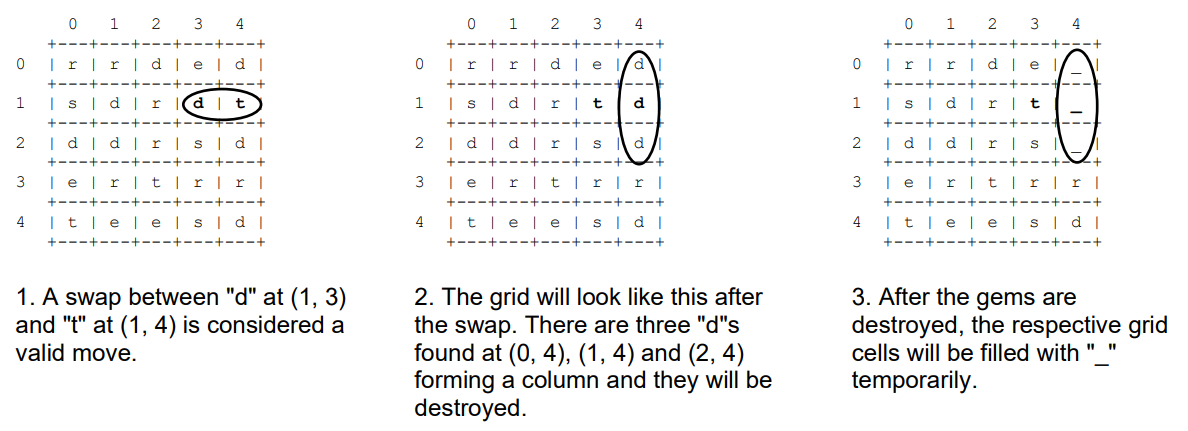
\includegraphics[width=0.7\paperwidth]{C:/Users/Admin/Desktop/Github/question_bank/LyX/static/img/9597-RVHS-2019-P1-Q4-1}
\par\end{center}

Some other valid swaps are: 
\begin{center}
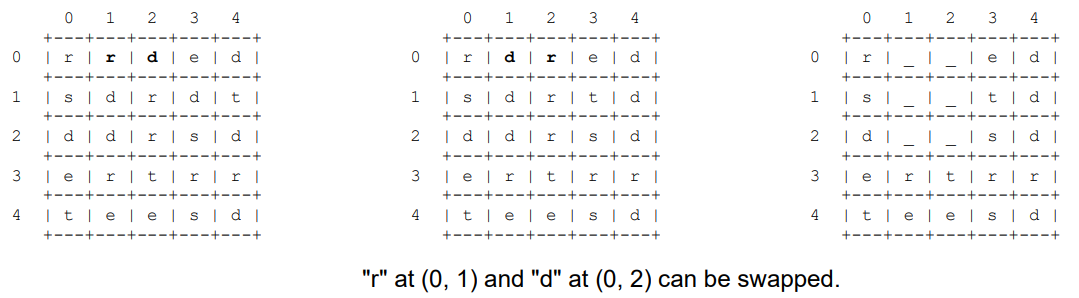
\includegraphics[width=0.7\paperwidth]{C:/Users/Admin/Desktop/Github/question_bank/LyX/static/img/9597-RVHS-2019-P1-Q4-2}
\par\end{center}

\begin{center}
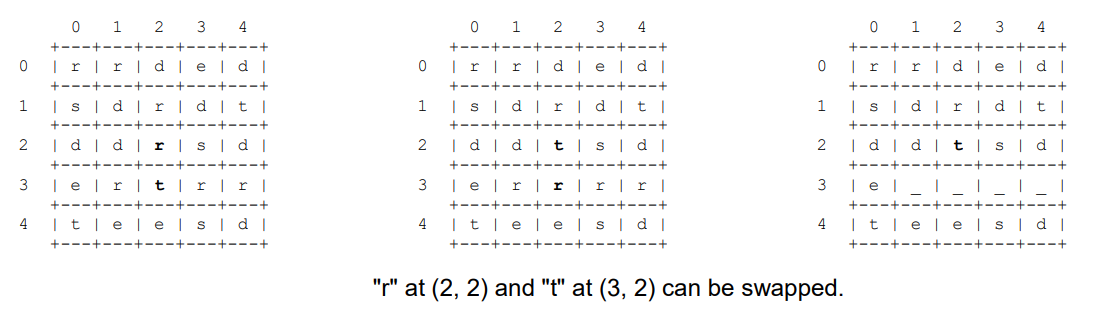
\includegraphics[width=0.7\paperwidth]{C:/Users/Admin/Desktop/Github/question_bank/LyX/static/img/9597-RVHS-2019-P1-Q4-3}
\par\end{center}

\begin{center}
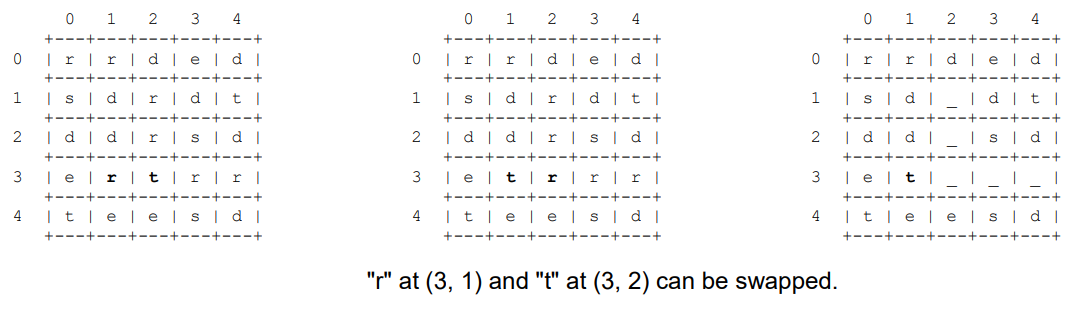
\includegraphics[width=0.7\paperwidth]{C:/Users/Admin/Desktop/Github/question_bank/LyX/static/img/9597-RVHS-2019-P1-Q4-4}
\par\end{center}

You are tasked to create a text-based interactive \textquotedblleft Begemed\textquotedblright{}
game in the following tasks. 

\subsection*{Task 4.1 }

Implement \texttt{Begemed} class according to the UML class diagram
and attributes/methods specifications given. 
\begin{center}
\begin{tabular}{|l|}
\hline 
\texttt{Board}\tabularnewline
\hline 
\texttt{- board: list }\tabularnewline
\hline 
\texttt{+ Board(size: int)}\tabularnewline
\texttt{+ new\_game(board: list) }\tabularnewline
\texttt{+ check\_connection(row: int, col: int): boolean }\tabularnewline
\texttt{+ find\_valid\_moves(row: int, col: int): list}\tabularnewline
\texttt{+ display(hint: boolean=False)}\tabularnewline
\hline 
\end{tabular}
\par\end{center}

\begin{center}
\begin{tabular}{|l|l|}
\hline 
\texttt{\textbf{Attribute}} & \texttt{\textbf{Specification}}\tabularnewline
\hline 
\texttt{board: list} & \texttt{board} is a 2-dimensional \texttt{list} hosting the gems inside
each grid. \tabularnewline
\hline 
\end{tabular}
\par\end{center}

Methods and its specification.
\begin{itemize}
\item \texttt{Board(n: int) : n} is the size used to define the dimension
of the \texttt{board}. The board should be initialized to a ($n\times n$)
2- dimensional list filled with string \textquotedblleft \_\textquotedblright .
\hfill{}{[}2{]}
\item \texttt{new\_game(new\_board : list): new\_game} takes in a \texttt{list}
named \texttt{new\_board} and assign it to the class attribute \texttt{board}.
The following list is provided in the python template file. 

t\texttt{est\_board = {[} {[}'r', 'r', 'd', 'e', 'd'{]}, {[}'s', 'd',
'r', 'd', 't'{]}, {[}'d', 'd', 'r', 's', 'd'{]}, {[}'e', 'r', 't',
'r', 'r'{]}, {[}'t', 'e', 'e', 's', 'd'{]}{]} }

\emph{This method is just a temporary solution which help you in initial
coding and debugging. In a later task, there will be further instructions
to update its implementation.} \hfill{}{[}1{]}
\item \texttt{check\_connection( row: int, col: int): boolean : check\_connection}
takes in the \texttt{row} and \texttt{col} value of a particular gem,
then check if there is a connection of 3 or more gems of the same
type in its horizontal or vertical direction. Return \texttt{True}
if such a connection is found, and \texttt{False} otherwise. \hfill{}{[}8{]}
\end{itemize}

\subsection*{Evidence 24 }

Program code of class Board and class methods up to \texttt{check\_conection}.
{[}11{]} 

Methods and its specification.
\begin{itemize}
\item \texttt{find\_valid\_moves( row: int, col: int): list} : \texttt{find\_valid\_moves}
takes in the \texttt{row} and \texttt{col} value of a particular gem,
then attempt to swap in the four directions (up, down, left, right).
If there is a new connection of 3 or more gems of the same type formed,
record as a valid movement. 

Return a \texttt{list} containing all valid movements. An empty \texttt{list}
is to be returned if no valid movement is found. 

For example:

\noindent %
\noindent\begin{minipage}[t]{1\columnwidth}%
\texttt{~~~~0~~~1~~~2~~~3~~~4 }

\texttt{~~+-{}-{}-+-{}-{}-+-{}-{}-+-{}-{}-+-{}-{}-+ }

\texttt{0 | r | r | d | e | d | }

\texttt{~~+-{}-{}-+-{}-{}-+-{}-{}-+-{}-{}-+-{}-{}-+ }

\texttt{1 | s | d | r | d | t | }

\texttt{~~+-{}-{}-+-{}-{}-+-{}-{}-+-{}-{}-+-{}-{}-+ }

\texttt{2 | d | d | r | s | d | }

\texttt{~~+-{}-{}-+-{}-{}-+-{}-{}-+-{}-{}-+-{}-{}-+ }

\texttt{3 | e | r | t | r | r | }

\texttt{~~+-{}-{}-+-{}-{}-+-{}-{}-+-{}-{}-+-{}-{}-+ }

\texttt{4 | t | e | e | s | d | }

\texttt{~~+-{}-{}-+-{}-{}-+-{}-{}-+-{}-{}-+-{}-{}-+ }%
\end{minipage}

If \texttt{find\_valid\_moves(0, 2)} is called, the function should
return \texttt{{[}'d', 'l'{]}} because when down swap or left swap
is performed on gem at \texttt{(0, 2)}, a new connection of 3 or more
gems of the same type will be formed. {[}5{]}
\item \texttt{display(hint: Boolean=False)} : \texttt{display} will print
out the \texttt{board} according to the sample format given. Take
note that the \texttt{size} of the board can be changed and hence
the grid outline should be dynamically adjusted according to its \texttt{size}. 

For example: 

\noindent %
\noindent\begin{minipage}[t]{1\columnwidth}%
\texttt{~~~~0~~~1~~~2~~~3~~~4}

\texttt{~~+-{}-{}-+-{}-{}-+-{}-{}-+-{}-{}-+-{}-{}-+}

\texttt{0 | r | r | d | e | d |}

\texttt{~~+-{}-{}-+-{}-{}-+-{}-{}-+-{}-{}-+-{}-{}-+}

\texttt{1 | s | d | r | d | t |}

\texttt{~~+-{}-{}-+-{}-{}-+-{}-{}-+-{}-{}-+-{}-{}-+}

\texttt{2 | d | d | r | s | d |}

\texttt{~~+-{}-{}-+-{}-{}-+-{}-{}-+-{}-{}-+-{}-{}-+}

\texttt{3 | e | r | t | r | r |}

\texttt{~~+-{}-{}-+-{}-{}-+-{}-{}-+-{}-{}-+-{}-{}-+}

\texttt{4 | t | e | e | s | d |}

\texttt{~~+-{}-{}-+-{}-{}-+-{}-{}-+-{}-{}-+-{}-{}-+}%
\end{minipage}

\texttt{hint} is an optional argument with a default value of \texttt{False}.
If \texttt{hint} is set to be \texttt{True}, the gems with valid moves
should be highlighted by using the \textbf{uppercase} letters, and
the valid moves for the \textbf{coordinates} and \textbf{directions}
should be displayed too. 

For example: 

\noindent %
\noindent\begin{minipage}[t]{1\columnwidth}%
\texttt{(0, 1) {[}'r'{]}}

\texttt{(0, 2) {[}'d', 'l'{]}}

\texttt{(1, 2) {[}'u'{]} }

\texttt{(1, 3) {[}'u', 'r'{]}}

\texttt{(2, 2) {[}'d'{]} }

\texttt{(3, 0) {[}'d'{]} }

\texttt{(3, 1) {[}'r'{]}}

\texttt{(3, 3) {[}'l'{]} }%
\end{minipage}

\noindent %
\noindent\begin{minipage}[t]{1\columnwidth}%
\texttt{~~~~0~~~1~~~2~~~3~~~4}

\texttt{~~+-{}-{}-+-{}-{}-+-{}-{}-+-{}-{}-+-{}-{}-+}

\texttt{0 | r | }\texttt{\textbf{\uline{R}}}\texttt{ | }\texttt{\textbf{\uline{D}}}\texttt{
| e | d |}

\texttt{~~+-{}-{}-+-{}-{}-+-{}-{}-+-{}-{}-+-{}-{}-+}

\texttt{1 | s | d | }\texttt{\textbf{\uline{R}}}\texttt{ | }\texttt{\textbf{\uline{D}}}\texttt{
| t |}

\texttt{~~+-{}-{}-+-{}-{}-+-{}-{}-+-{}-{}-+-{}-{}-+}

\texttt{2 | d | d | }\texttt{\textbf{\uline{R}}}\texttt{ | s |
d |}

\texttt{~~+-{}-{}-+-{}-{}-+-{}-{}-+-{}-{}-+-{}-{}-+}

\texttt{3 | }\texttt{\textbf{\uline{E}}}\texttt{ | }\texttt{\textbf{\uline{R}}}\texttt{
| t | }\texttt{\textbf{\uline{R}}}\texttt{ | r |}

\texttt{~~+-{}-{}-+-{}-{}-+-{}-{}-+-{}-{}-+-{}-{}-+}

\texttt{4 | t | e | e | s | d |}

\texttt{~~+-{}-{}-+-{}-{}-+-{}-{}-+-{}-{}-+-{}-{}-+}%
\end{minipage}
\end{itemize}

\subsection*{Evidence 25 }

Program code of class method \texttt{find\_valid\_moves} and \texttt{display}.
\hfill{}{[}14{]}

\subsection*{Task 4.2 }

Write a texted based menu which has the following options. Validation
of the user input is needed. 

\noindent %
\noindent\begin{minipage}[t]{1\columnwidth}%
\texttt{Choose an option below: }

\texttt{1) Validate Move }

\texttt{2) Toggle Hint Mode}

\texttt{3) Move the Gem!}

\texttt{4) New Game}

\texttt{5) Exit }%
\end{minipage}

The descriptions for the options can be found below. 

Options and its descriptions.
\begin{itemize}
\item \texttt{Validate Move} : Ask user to input a set of \texttt{row},
\texttt{col} and \texttt{direction}. Check and feedback if this swap
is valid. 
\item \texttt{Toggle Hint Mode} : For every new game, the \texttt{hint}
mode by default should be \texttt{off}. Use this option to toggle
the \texttt{on} and \texttt{off} state of hint mode.

If \texttt{hint} mode is \texttt{on}, the menu interface should automatically
highlight the gems with valid moves and print out a list of the coordinates
together with its valid movement directions. 
\item \texttt{Move the Gem! :} Move a gem in a chosen direction. 

\emph{Note that the related class method will only be implemented
in the }\textbf{\emph{next task}}\emph{. For the current menu, you
only need to take in user input for }\texttt{row}\emph{, }\texttt{col}\emph{
and }\texttt{direction}\emph{, but no further action needs to be taken. }
\item \texttt{New Game} : Start a new game and reset \texttt{hint} mode
to be off. 

For this task, you may just initialize the new game using the \texttt{test\_board}
given. 
\item \texttt{Exit} : Exit program. 
\end{itemize}

\subsection*{Evidence 26}

Program code of menu implementation. \hfill{}{[}10{]}

\subsection*{Task 4.3}

Update the class Begemed with the following methods. Note that this
task is time consuming and only worth \textbf{2 marks}. 

Methods and its specification.
\begin{itemize}
\item \texttt{new\_game(n: int)} : \texttt{new\_game} will now take in a
size of \texttt{n} and randomly generate a \texttt{$\mathtt{n}\times\mathtt{n}$}
board of gems. The newly generated gems should not have any connection
of 3 or more gems with the same type. 
\item \texttt{move\_gem(row: int, col: int, direction: string)} \texttt{move\_gem}
should take in a gem position and direction. If the swap is a valid
move, detect any newly formed connection of 3 or more gems with the
same type and cancel them. 

\noindent %
\begin{minipage}[t]{0.5\columnwidth}%
\texttt{~~~~0~~~1~~~2~~~3~~~4 }

\texttt{~~+-{}-{}-+-{}-{}-+-{}-{}-+-{}-{}-+-{}-{}-+ }

\texttt{0 | r | r | d | e | d |}

\texttt{~~+-{}-{}-+-{}-{}-+-{}-{}-+-{}-{}-+-{}-{}-+ }

\texttt{1 | s | d | r | d | t |}

\texttt{~~+-{}-{}-+-{}-{}-+-{}-{}-+-{}-{}-+-{}-{}-+ }

\texttt{2 | d | d | r | s | d |}

\texttt{~~+-{}-{}-+-{}-{}-+-{}-{}-+-{}-{}-+-{}-{}-+ }

\texttt{3 | e | }\texttt{\textbf{\uline{r}}}\texttt{ | }\texttt{\textbf{\uline{t}}}\texttt{
| r | r |}

\texttt{~~+-{}-{}-+-{}-{}-+-{}-{}-+-{}-{}-+-{}-{}-+ }

\texttt{4 | t | e | e | s | d |}

\texttt{~~+-{}-{}-+-{}-{}-+-{}-{}-+-{}-{}-+-{}-{}-+}

Swap \textquotedbl r\textquotedbl{} at (3, 1) with \textquotedbl t\textquotedbl{}
at (3, 2)%
\end{minipage}%
\begin{minipage}[t]{0.5\columnwidth}%
\texttt{~~~~0~~~1~~~2~~~3~~~4 }

\texttt{~~+-{}-{}-+-{}-{}-+-{}-{}-+-{}-{}-+-{}-{}-+}

\texttt{0 | r | r | d | e | d | }

\texttt{~~+-{}-{}-+-{}-{}-+-{}-{}-+-{}-{}-+-{}-{}-+ }

\texttt{1 | s | d | \_ | d | t |}

\texttt{~~+-{}-{}-+-{}-{}-+-{}-{}-+-{}-{}-+-{}-{}-+ }

\texttt{2 | d | d | \_ | s | d | }

\texttt{~~+-{}-{}-+-{}-{}-+-{}-{}-+-{}-{}-+-{}-{}-+ }

\texttt{3 | e | t | \_ | \_ | \_ | }

\texttt{~~+-{}-{}-+-{}-{}-+-{}-{}-+-{}-{}-+-{}-{}-+ }

\texttt{4 | t | e | e | s | d | }

\texttt{~~+-{}-{}-+-{}-{}-+-{}-{}-+-{}-{}-+-{}-{}-+}

Gems connected with 3 or more of the same type are cancelled. %
\end{minipage}

After the gems are being cancelled, those gems on top of the current
gems should \textquotedblleft fall\textquotedblright{} down. 

New gems will be randomly generated to fill up the board. 

\noindent %
\begin{minipage}[t]{0.5\columnwidth}%
\texttt{~~~~0~~~1~~~2~~~3~~~4 }

\texttt{~~+-{}-{}-+-{}-{}-+-{}-{}-+-{}-{}-+-{}-{}-+ }

\texttt{0 | r | r | \_ | \_ | \_ | }

\texttt{~~+-{}-{}-+-{}-{}-+-{}-{}-+-{}-{}-+-{}-{}-+ }

\texttt{1 | s | d | \_ | }\texttt{\textbf{\uline{e}}}\texttt{ |
}\texttt{\textbf{\uline{d}}}\texttt{ |}

\texttt{~~+-{}-{}-+-{}-{}-+-{}-{}-+-{}-{}-+-{}-{}-+ }

\texttt{2 | d | d | \_ | }\texttt{\textbf{\uline{d}}}\texttt{ |
}\texttt{\textbf{\uline{t}}}\texttt{ |}

\texttt{~~+-{}-{}-+-{}-{}-+-{}-{}-+-{}-{}-+-{}-{}-+ }

\texttt{3 | e | t | }\texttt{\textbf{\uline{d}}}\texttt{ | }\texttt{\textbf{\uline{s}}}\texttt{
| }\texttt{\textbf{\uline{d}}}\texttt{ |}

\texttt{~~+-{}-{}-+-{}-{}-+-{}-{}-+-{}-{}-+-{}-{}-+ }

\texttt{4 | t | e | e | s | d | }

\texttt{~~+-{}-{}-+-{}-{}-+-{}-{}-+-{}-{}-+-{}-{}-+ }

Gems on top of the cancelled gem \textquotedblleft falls\textquotedblright{}
down%
\end{minipage}%
\begin{minipage}[t]{0.5\columnwidth}%
\texttt{~~~~0~~~1~~~2~~~3~~~4 }

\texttt{~~+-{}-{}-+-{}-{}-+-{}-{}-+-{}-{}-+-{}-{}-+ }

\texttt{0 | r | r | }\texttt{\textbf{\uline{r}}}\texttt{ | }\texttt{\textbf{\uline{s}}}\texttt{
| }\texttt{\textbf{\uline{s}}}\texttt{ |}

\texttt{~~+-{}-{}-+-{}-{}-+-{}-{}-+-{}-{}-+-{}-{}-+ }

\texttt{1 | s | d | }\texttt{\textbf{\uline{t}}}\texttt{ | e |
d | }

\texttt{~~+-{}-{}-+-{}-{}-+-{}-{}-+-{}-{}-+-{}-{}-+ }

\texttt{2 | d | d | }\texttt{\textbf{\uline{t}}}\texttt{ | d |
t | }

\texttt{~~+-{}-{}-+-{}-{}-+-{}-{}-+-{}-{}-+-{}-{}-+ }

\texttt{3 | e | t | d | s | d |}

\texttt{~~+-{}-{}-+-{}-{}-+-{}-{}-+-{}-{}-+-{}-{}-+ }

\texttt{4 | t | e | e | s | d |}

\texttt{~~+-{}-{}-+-{}-{}-+-{}-{}-+-{}-{}-+-{}-{}-+ }

New gems are generated %
\end{minipage}

Check if there are more connections of 3 or more gems of the same
type are formed, if found repeat the above cancel and refill steps. 
\item \texttt{menu} Adjust the menu to accommodate these new changes. 
\end{itemize}

\subsection*{Evidence 27 }

Program code of above mentioned changes. \hfill{}{[}2{]}

 \newpage 

\item \textbf{{[}RVHS/PRELIM/9597/2019/P2/Q1{]} }

Vending machine
\begin{enumerate}
\item Draw a data flow diagram for a vending machine system that allows
user to buy drinks using coins and seller to refill stock. \emph{Note:
You are to decide on the processes to be included in the DFD on your
own}. \hfill{}{[}5{]}
\item Draw a flow chart on the steps in dispensing a drink by the vending
machine. Your flow chart should include various situations faced by
the system e.g. not enough cash, drinks chosen out of stock etc. \hfill{}{[}5{]}
\end{enumerate}

 \newpage 

\item \textbf{{[}RVHS/PRELIM/9597/2019/P2/Q2{]} }

Driverless car
\begin{enumerate}
\item State one ethical and one social issue of using driverless car. \hfill{}{[}2{]}
\item A simplified decision making on the behavior of a driverless car is
as follow. 
\begin{itemize}
\item When a pedestrian is sensed 10m ahead, the driverless car \textbf{must}
apply emergency break if its current speed is more than 20 km/hr.
Otherwise, it should slow down gently.
\item In other situations, when red light is sensed 20m ahead, the driverless
car should slow down gently regardless of its speed. 
\end{itemize}
Draw a reduced decision table for the scenario above. \hfill{}{[}5{]}
\end{enumerate}

 \newpage 

\item \textbf{{[}RVHS/PRELIM/9597/2019/P2/Q3{]} }

A project manager uses the PERT chart to manage a software project.
\begin{center}
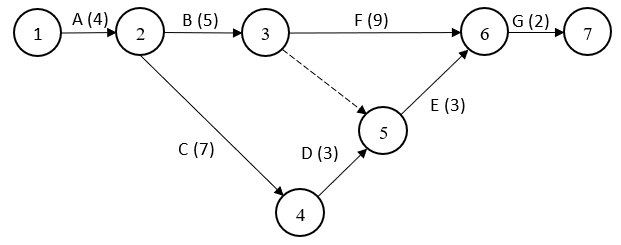
\includegraphics[width=0.5\paperwidth]{C:/Users/Admin/Desktop/Github/question_bank/LyX/static/img/9597-RVHS-2019-P2-Q3-1}
\par\end{center}

\noindent \begin{center}
\begin{tabular}{|c|c|c|}
\hline 
\textbf{Activity} & \textbf{Description} & \textbf{Duration (week)}\tabularnewline
\hline 
A & Specification & 4\tabularnewline
\hline 
B & Installation of datastore servers & 5\tabularnewline
\hline 
C & Development & 7\tabularnewline
\hline 
D & Unit Testing & 3\tabularnewline
\hline 
E & System testing & 3\tabularnewline
\hline 
F & Conversion of existing data files to new format & 9\tabularnewline
\hline 
G & UAT & 2\tabularnewline
\hline 
\end{tabular}
\par\end{center}
\begin{enumerate}
\item Explain the significance of the dotted line. \hfill{}{[}1{]}
\item Draw a Gantt chart based on the above information.\hfill{} {[}3{]}
\item State the impact on the project if activity F duration is cut by 3
weeks.\hfill{} {[}2{]}
\item State the purpose of the project proposal.\hfill{} {[}1{]}
\item State 2 important topics in the project proposal. \hfill{}{[}1{]}
\end{enumerate}

 \newpage 

\item \textbf{{[}RVHS/PRELIM/9597/2019/P2/Q4{]} }

A user-defined linked list has the following operations.

Operations and its descriptions 
\begin{itemize}
\item \texttt{create()} : This function creates an empty linked list.

For example: 

\texttt{lst1 = create()}

A linked list is created and referenced by \texttt{lst1}.
\item \texttt{insert(llst,data)} : This procedure always adds \texttt{data}
as a node at the head of the linked list

For example

\noindent %
\noindent\begin{minipage}[t]{1\columnwidth}%
\texttt{lst1: 'A'->'B'->'C'->'D'->'E'}

\texttt{insert(lst1, 'Z')}

\texttt{lst1: 'Z'->'A'->'B'->'C'->'D'->'E'}%
\end{minipage}
\item \texttt{split(llst,pos)} The function breaks the linked list at position
\texttt{pos} and returns the cut half as a new linked list.

For example: 

\noindent %
\noindent\begin{minipage}[t]{1\columnwidth}%
\texttt{lst1: 'A'->'B'->'C'->'D'->'E'}

\texttt{lst2 = split(lst1, 2)}

\texttt{lst1: 'A'->'B' }

\texttt{lst2: 'C'->'D'->'E'}%
\end{minipage}
\item \texttt{join(llst1,llist2)} This function joins 2 linked lists as
one.

For example: 

\noindent %
\noindent\begin{minipage}[t]{1\columnwidth}%
\texttt{lst1: 'C'->'B' }

\texttt{lst2: 'A'->'D'->'E}

\texttt{join(lst1, lst2)}

\texttt{lst1: 'C'->'B'->'A'->'D'->'E' }

\texttt{lst2: Empty}%
\end{minipage}
\end{itemize}
Using the provided operations of the linked list, write, in pseudo-code
an algorithm that could be used to implement the \texttt{swap} operation.
\emph{Hint: you don\textquoteright t have to use all the operations
provided}.

Operations and its description 
\begin{itemize}
\item \texttt{swap(llst,pos)} : This procedure swaps the data at positions
\texttt{pos} and \texttt{pos + 1}

For example: 

\noindent %
\noindent\begin{minipage}[t]{1\columnwidth}%
\texttt{lst1:'A'->'B'->'C'->'D'->'E' }

\texttt{swap(lst1,3)}

\texttt{lst1:'A'->'B'->'D'->'C'->'E'}%
\end{minipage}
\end{itemize}
You can assume that the operations executed are always valid. For
example, if there is no 5th node, \texttt{swap(lst1,4)} will not be
called. \hfill{}{[}5{]}

 \newpage 

\item \textbf{{[}RVHS/PRELIM/9597/2019/P2/Q5{]} }

Computer Network
\begin{enumerate}
\item Explain how the switch forwards data packet to destinated device.
\hfill{}{[}1{]}
\item State the function of a router.\hfill{} {[}1{]}
\item Explain with an example what a client server network is.\hfill{}
{[}1{]}
\item Describe the differences between PaaS and IaaS.\hfill{} {[}1{]}
\item State 2 data verification methods.\hfill{} {[}1{]}
\item Explain what packet switching is.\hfill{} {[}1{]}
\item State the connection mode that the walkie-talkie (push to talk) is
working on.\hfill{} {[}1{]}
\item State the difference between synchronous and asynchronous data transmission.
\hfill{}{[}1{]}
\item State and explain a method to protect data in transit.\hfill{} {[}1{]}
\item State and explain a method to protect data at rest.\hfill{}{[}1{]}
\end{enumerate}

 \newpage 

\item \textbf{{[}RVHS/PRELIM/9597/2019/P2/Q6{]} }

A sort procedure is implemented in Python is follow.

\noindent %
\noindent\begin{minipage}[t]{1\columnwidth}%
\texttt{def sort(sort\_lst, unsort\_lst):}

\texttt{\qquad{}if len(unsort\_lst) > 0: }

\texttt{\qquad{}\qquad{}item = unsort\_lst{[}0{]} }

\texttt{\qquad{}\qquad{}i = 0 }

\texttt{\qquad{}\qquad{}while i < len(sort\_lst) and item < sort\_lst{[}i{]}: }

\texttt{\qquad{}\qquad{}\qquad{}i += 1 }

\texttt{\qquad{}\qquad{}return sort(sort\_lst{[}:i{]}+{[}item,{]}+sort\_lst{[}i:{]},
unsort\_lst{[}1:{]})}

\texttt{\qquad{}else:}

\texttt{\qquad{}\qquad{}return sort\_lst}%
\end{minipage}
\begin{enumerate}
\item State the name of the above sorting algorithm. \hfill{}{[}1{]}
\item The below statement is executed.

\texttt{>\textcompwordmark >\textcompwordmark > sort({[}{]}, {[}9,1,8,2,3,7,5{]})}

Using the table below, trace the items in \texttt{sort\_lst} and \texttt{unsort\_lst}
in each recursive call.
\noindent \begin{center}
\begin{tabular}{|c|c|c|}
\hline 
\texttt{\textbf{\#}} & \texttt{\textbf{sort\_lst}} & \texttt{\textbf{unsort\_lst}}\tabularnewline
\hline 
\texttt{1} & \texttt{{[}{]}} & \texttt{{[}9,1,8,2,3,7,5{]}}\tabularnewline
\hline 
\texttt{2} &  & \tabularnewline
\hline 
\texttt{3} &  & \tabularnewline
\hline 
\texttt{4} &  & \tabularnewline
\hline 
\texttt{5} &  & \tabularnewline
\hline 
\texttt{6} &  & \tabularnewline
\hline 
\texttt{7} &  & \tabularnewline
\hline 
\texttt{8} &  & \tabularnewline
\hline 
\end{tabular}
\par\end{center}

\hfill{}{[}3{]}
\item State the time complexity of the sort procedure above. \hfill{}{[}1{]}
\end{enumerate}
\quad{} A sleepy teacher implemented an inefficient binary search
function as follow. The function is supposed to return True if target
is found in the list inc\_sort\_lst and False otherwise.

\noindent %
\noindent\begin{minipage}[t]{1\columnwidth}%
\texttt{01 def binSearch(target, inc\_sort\_lst):}

\texttt{02 if len(inc\_sort\_lst) == 0: }

\texttt{03 \qquad{}return False}

\texttt{04 if len(inc\_sort\_lst) == 1: }

\texttt{05 \qquad{}return True }

\texttt{06 n = len(inc\_sort\_lst)}

\texttt{07 first\_half = inc\_sort\_lst{[}:n//2{]} }

\texttt{08 second\_half = inc\_sort\_lst{[}n//2:{]} }

\texttt{09 if target > first\_half{[}-1{]}: }

\texttt{10 \qquad{}return binSearch(target, second\_half) }

\texttt{11 else: }

\texttt{12 \qquad{}return binSearch(target, first\_half)}%
\end{minipage}
\begin{enumerate}
\item[(d)]  Explain the bug in his code with examples. \hfill{}{[}1{]}
\item[(e)]  Explain how you can correct the bug without changing the code from
line 06 onwards.\hfill{} {[}2{]}
\item[(f)]  Explain why the binary search performed is inefficient.\hfill{}
{[}2{]}
\end{enumerate}

 \newpage 

\item \textbf{{[}RVHS/PRELIM/9597/2019/P2/Q7{]} }

Run length encoding (RLE) is a very simple form of lossless data compression
which runs on sequences having same value occurring many consecutive
times and it encodes the sequence to store only a single value and
its count. For example, \textquotedblleft 111111000\textquotedblright{}
can be converted to \textquotedblleft 6130\textquotedblright .

Below is a draft attempt of implementing this algorithm. 

\noindent %
\noindent\begin{minipage}[t]{1\columnwidth}%
\texttt{01 PROCEDURE RLECompress(s: STRING): }

\texttt{02 \qquad{}DECLARE comp\_str: STRING }

\texttt{03 \qquad{}DECLARE count, i: INT }

\texttt{04 \qquad{}comp\_str = \textquotedbl\textquotedbl{} }

\texttt{05 \qquad{}count, i = 0, 0 }

\texttt{06 }

\texttt{07 \qquad{}WHILE i < LENGTH(s): }

\texttt{08 \qquad{}\qquad{}count = 1 }

\texttt{09 }

\texttt{10 \qquad{}\qquad{}WHILE i < LENGTH(s) - 1 and s{[}i{]}
== s{[}i+1{]}:}

\texttt{11 \qquad{}\qquad{}\qquad{}count += 1 }

\texttt{12 \qquad{}\qquad{}\qquad{}i += 1 }

\texttt{13 \qquad{}\qquad{}END WHILE }

\texttt{14 }

\texttt{15 \qquad{}\qquad{}comp\_str += count + s{[}i{]} }

\texttt{16 \qquad{}END WHILE }

\texttt{17 }

\texttt{18 \qquad{}RETURN comp\_str }

\texttt{19 END PROCEDURE}%
\end{minipage}
\begin{enumerate}
\item The compiler reported an error at line 15. Identity the type of error,
state its definition and suggest how it can be fixed.\hfill{} {[}3{]}
\item After the above error has been corrected, a successful compilation
produces executable code. However, when the code was executed, it
failed to complete. Identity another type of error, state its definition
and suggest how it can be fixed. \hfill{}{[}3{]}
\end{enumerate}
Assuming all errors have been identified and corrected.

The following steps are taken to encode English alphabets:
\begin{enumerate}
\item[1.]  Convert alphabet to hexadecimal ASCII value 
\item[2.]  Convert the hexadecimal number to binary number 
\item[3.]  Encode the binary number using RLE algorithm
\end{enumerate}
For example, the alphabet \textquotedblleft A\textquotedblright{}
has a hexadecimal ASCII value of \textquotedblleft 41\textquotedblright .
\begin{enumerate}
\item[(c)]  State the definition of ASCII.\hfill{} {[}2{]}
\item[(d)]  State the encoded RLE string for letter \textquotedblleft A\textquotedblright .\hfill{}
{[}1{]}
\item[(e)]  State and explain with example one potential limitation of RLE encoding
when compressing long binary strings. \hfill{}{[}2{]}
\end{enumerate}

 \newpage 

\item \textbf{{[}RVHS/PRELIM/9597/2019/P2/Q8{]} }

The school library currently stores their data in flat files. These
files contain information about students, books and their loaning
details. 

Using examples from the school\textquoteright s flat files to illustrate
your answers.
\begin{enumerate}
\item Explain how data inconsistency could arise.\hfill{} {[}2{]}
\item Explain why data privacy could be a potential concern.\hfill{} {[}2{]}
\item Explain the definition of Primary Key in a relational database. \hfill{}{[}2{]}
\end{enumerate}
A book can be borrowed by any student, and a student can borrow any
book. Students need to fill up a loaning record form each time he/she
wants to borrow a book. A student is entitled to borrow up to 5 books
each time using the same loaning record form.

The decision has been made to create a relational database for the
library loaning system.
\begin{enumerate}
\item[(d)]  Identify the necessary tables and draw an E-R diagram to show the
relationships between these tables. {[}4{]}
\item[(e)]  For each table specify the attributes (fields) required and state
suitable primary keys and foreign key relationships. State necessary
legends if you are using symbols to represent the primary and foreign
keys. {[}7{]}
\end{enumerate}
The following table is generated for students\textquoteright{} reference
regarding their loaning details.

\begin{tabular}{|l|l|l|l|}
\hline 
\textbf{Student Name:} & Xiao Ming  & \textbf{Class: } & 19J08\tabularnewline
\hline 
 &  &  & \tabularnewline
\hline 
\textbf{Book Name} & \textbf{Author} & \textbf{Loan Date} & \textbf{Due Date}\tabularnewline
\hline 
A Brief History of Time & Stephen Hawking & 05 Aug 2019 & 30 Aug 2019\tabularnewline
\hline 
Spider Man Comics & Stan Lee & 29 Aug 2019 & 20 Sep 2019\tabularnewline
\hline 
\end{tabular}
\begin{enumerate}
\item[(f)]  To create the report \texttt{StudentName} and \texttt{StudentClass}
are used. Name other fields that the database uses to produce this
report.\hfill{}{[}4{]}
\end{enumerate}
Beside the database design, you are also in charge of creating an
online loaning form.
\begin{enumerate}
\item[(g)]  Design and draw a webpage layout for the auto loaning interface
for the new system. Identify and briefly explain your design considerations
for the various features which aid users to input valid data entries.
\hfill{}{[}4{]}
\item[(h)]  Some students use their handphones to snap photos of tables and
charts from the books they borrowed and use them for their research
projects. Explain what potential issues may arise and suggest alternate
ways which students can adopt.\hfill{} {[}3{]}
\end{enumerate}

 \newpage 

\item \textbf{{[}RVHS/PRELIM/9597/2019/P2/Q9{]} }

The school library has in store different kinds of items which students
can loan out. Information about items are stored and recorded, such
as \texttt{title}, \texttt{description}, and \texttt{damaged}, which
is a Boolean value indicating if the item has any form of physical
damage.

For books in the library, additional information such as the \texttt{author},
\texttt{publisher}, \texttt{ISBN} are recorded.

Digital media resources are also available for students\textquoteright{}
reference. Information such as \texttt{storage media}, \texttt{file
size} and\texttt{ playback time} are stored. 

You are engaged by the school to design an Object-Oriented Programming
solution to manage these items.
\begin{enumerate}
\item Draw a class diagram, with base class \texttt{Item}, showing: 
\begin{itemize}
\item appropriate sub-classes 
\item inheritance
\item the properties required 
\item appropriate methods, including \textbf{constructor} methods, and at
least \textbf{one} pair of \textquoteleft \textbf{get}\textquoteright{}
and \textquoteleft \textbf{set}\textquoteright{} methods for one of
the properties. \hfill{}{[}5{]}
\end{itemize}
\item Using the above example, explain the meaning of the term \textbf{Polymorphism}.
\hfill{}{[}2{]}
\item Using the above example, explain the meaning of the term \textbf{Encapsulation}.\hfill{}
{[}2{]}
\item The school also provides a series of past year examination papers
for the students\textquoteright{} loaning and reference. State how
this would affect the \textbf{class}, \textbf{properties} and \textbf{methods}
in the current example. \hfill{}{[}2{]}
\end{enumerate}

 \newpage 

\item \textbf{{[}YIJC/PRELIM/9597/2019/P1/Q1{]} }

According to some researches done on children below the age of 16,
it was found that the height of a boy, measured in centimetres (cm),
should lie within the normal range with: 
\noindent \begin{center}
minimum height = 5.3 \texttimes{} Age + 71 
\par\end{center}

\noindent \begin{center}
maximum height = 6.2 \texttimes{} Age + 87 
\par\end{center}

The text file HEIGHTDATA.TXT contains 20 entries of the data in the
following format: 
\noindent \begin{center}
<Name>, <Age>, <Height> 
\par\end{center}

\subsection*{Task 1.1: }

Write program code to:
\begin{itemize}
\item read the entire contents of \texttt{HEIGHTDATA.TXT}. 
\item determine if the boy\textquoteright s height lies within the normal
range. 
\item display the contents using the format given below 
\end{itemize}
\noindent %
\begin{minipage}[t]{0.5\columnwidth}%
Example run of the program: 

\textbf{Input File: }

\texttt{Ali,6,105 }

\texttt{Bob,10,145 }

\texttt{Charlie,15,185} %
\end{minipage}%
\fbox{\begin{minipage}[t]{0.5\columnwidth}%
The output generated from the input file would be: 

\texttt{\textbf{Name ~~~Age Height Within normal range }}

\texttt{Ali ~~~~6 ~~105 ~~~Yes}

\texttt{Bob ~~~~10 ~145 ~~~Yes }

\texttt{Charlie 15 ~185 ~~~No}%
\end{minipage}}

\subsection*{Evidence 1.1: }

Your program code. \hfill{}{[}6{]}

\subsection*{Evidence 1.2: }

Screenshot of the output.\hfill{} {[}2{]}

During data entry, some of the data may have been wrongly entered
with transposition errors. In the case of Charlie\textquoteright s,
his height should have been 158 cm but was wrongly transposed and
entered as 185 cm. 

\subsection*{Task 1.2: }

Write program code to: 
\begin{itemize}
\item determine the correct height for those entries outside the normal
range. 
\item display the amended contents using the format given below. 
\end{itemize}
In cases where there are more than one possible or no possible height,
print \textquoteleft Re-enter data\textquoteright .

\noindent %
\begin{minipage}[t]{0.5\columnwidth}%
Example run of the program:

\textbf{Input File:}

\texttt{Ali,6,105}

\texttt{Bob,10,145 }

\texttt{Charlie,15,185 }

\texttt{Ethan,7,131 }

\texttt{Rick,13,415 }%
\end{minipage}%
\fbox{\begin{minipage}[t]{0.5\columnwidth}%
The output generated from the input file would be:

\texttt{\textbf{Name ~~~Age Height Corrected Height}}

\texttt{Charlie 15 ~185 ~~~158}

\texttt{Ethan ~~7 ~~131 ~~~113 }

\texttt{Rick ~~~13 ~415 ~~~Re-enter data}%
\end{minipage}}

Example run of the program: 

\subsection*{Evidence 1.3: }

Your program code. \hfill{}{[}6{]}

\subsection*{Evidence 1.4: }

Screenshot of the output. \hfill{}{[}1{]}

 \newpage 

\item \textbf{{[}YIJC/PRELIM/9597/2019/P1/Q2{]} }

The Oxford English Dictionary, published in 1989, contains 171,476
words. Instead of doing a linear search whenever we want to find a
word, it is more efficient to perform a binary search. 

\subsection*{Evidence 2.1: }

Describe the binary search algorithm. \hfill{}{[}2{]}

\subsection*{Task 2.1: }

Write a program \texttt{BinarySearch(lst, item)} to search for an
item in the list \texttt{lst} using the binary search algorithm. 

The program will:
\begin{itemize}
\item import the sorted list of words, given in the file \texttt{1000WORDS.TXT},
into a simple array \texttt{dataset}. 
\item report whether or not the item is found in the list. If found, output
the index position and the list of words examined by the program during
the binary search. 
\end{itemize}

\subsection*{Evidence 2.2:}

Your program code and the screenshot for the following searches: 
\begin{itemize}
\item \texttt{BinarySearch(dataset, \textquotedbl WORD\textquotedbl ) }
\item \texttt{BinarySearch(dataset, \textquotedbl WORDA\textquotedbl ) }
\item \texttt{BinarySearch(dataset, \textquotedbl TRADE\textquotedbl )}
\hfill{}{[}8{]}
\end{itemize}
If we want to find all the words that start with \textquotedblleft TR\textquotedblright ,
we can perform a partial word search on the given dataset. The search
will return a word list as follows: 
\noindent \begin{center}
\texttt{{[}'TRACK', 'TRADE', 'TRAIN', 'TRAVEL', 'TREE', 'TRIANGLE',
'TRIP', 'TROUBLE', 'TRUCK', 'TRUE', 'TRY'{]}}
\par\end{center}

Using the program written in Task 2.1 to perform a binary search for
the word \textquotedblleft \texttt{TR}\textquotedblright ; the first
word starting with \textquotedblleft \texttt{TR}\textquotedblright{}
should be \textquotedblleft \texttt{TRADE}\textquotedblright{} found
at index \texttt{889}. We can now perform a linear search near index
\texttt{889} for all the words starting with \textquotedblleft \texttt{TR}\textquotedblright . 

\subsection*{Task 2.2: }

Modify the code \texttt{BinarySearch(lst, item)} written in Task 2.1. 

Your program will: 
\begin{enumerate}
\item[1.]  perform a partial search for the word in the list \texttt{lst} starting
with the given letter(s), item 
\item[2.]  perform a linear search near the index found in step (1) to return
a list of words starting with the given letter(s) 
\end{enumerate}

\subsection*{Evidence 2.3: }

Your program code and the screenshot for the following searches: 
\begin{itemize}
\item \texttt{BinarySearch(dataset, \textquotedbl TR\textquotedbl )} 
\item \texttt{BinarySearch(dataset, \textquotedbl RE\textquotedbl )}\hfill{}
{[}5{]}
\end{itemize}

 \newpage 

\item \textbf{{[}YIJC/PRELIM/9597/2019/P1/Q3{]} }

An \texttt{ExpressionTree} data structure is required to store 20
nodes. A linked list is maintained of all the nodes. A node contains
a data value and two pointers: a left pointer and a right pointer.
Items in the list are initially linked using their \texttt{LeftChild}
pointers. 

Each node is implemented as an instance of the class \texttt{Node}. 

The class \texttt{Node} has the following properties: Class: Node
Attributes Identifier Data Type Description DataValue STRING The node
data LeftChild INTEGER The left node pointer RightChild INTEGER The
right node pointer 

The \texttt{ExpressionTree} class is implemented as follows: Class:
ExpressionTree Attributes Identifier Data Type Description Tree ARRAY{[}1:20{]}
OF Node The tree data, initialised as a linked list Fringe ARRAY:
INTEGER A list to store the index of nodes traversed Root INTEGER
Index for the root position of the Tree array NextFreeChild INTEGER
Index for the next unused node 

The index of the first available node is indicated by \texttt{NextFreeChild}.
The initial value of \texttt{Root} is 0 and the initial value of \texttt{NextFreeChild}
is 0. The \texttt{Fringe} is initialised as an empty list and it will
be used for node insertion to store the index for the nodes traversed. 

The diagram shows the \texttt{Tree} array with the linked list to
record the unused nodes.
\begin{center}
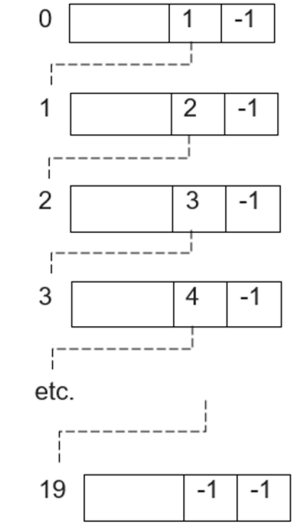
\includegraphics[width=0.15\paperwidth]{C:/Users/Admin/Desktop/Github/question_bank/LyX/static/img/9597-YIJC-2019-P1-Q3-1}
\par\end{center}

\subsection*{Task 3.1 }

Write a program code to define the \texttt{Node} and \texttt{ExpressionTree}
classes.

\subsection*{Evidence 3.1}

Your program code for Task 3.1. \hfill{}{[}12{]}

The task is to store the tokens of a binary arithmetic expression
in the data structure instantiated from the \texttt{ExpressionTree}
class. 

An arithmetic expression is a sequence of tokens that follows prescribed
rules. A token may be either an operand or an operator. 

A binary arithmetic operation using the standard arithmetic operators,
\texttt{+ - {*} /} , may be in the form of operand-operator-operand.
For example, 
\noindent \begin{center}
\texttt{2 + 3 }
\par\end{center}

where \texttt{2} and \texttt{3} are operands, \texttt{+} is an operator.
This expression will evaluate to a value of \texttt{5}. 

\subsection*{Task 3.2 }

Write a function \texttt{IsOperator(s)} that takes in a string \texttt{s},
and returns \texttt{True} if it is a standard arithmetic operator
and returns \texttt{False} if otherwise. 

\subsection*{Evidence 3.2 }

Your program code for Task 3.2. \hfill{}{[}2{]}

An expression tree is a binary tree with the following properties: 
\begin{enumerate}
\item[1.]  Each leaf is an \emph{operand}. 
\item[2.]  The root and internal nodes are \emph{operators}. 
\item[3.]  Subtrees are sub-expressions, with the root being an \emph{operator}.
\end{enumerate}
The following shows a series of commands to create and insert values
into the data structure to create an expression tree. 

\begin{minipage}[t]{0.5\columnwidth}%
\texttt{CreateNewExpTree }

\texttt{InsertToExpTree(\textquotedbl +\textquotedbl ) }

\texttt{InsertToExpTree(\textquotedbl{*}\textquotedbl ) }

\texttt{InsertToExpTree(\textquotedbl 4\textquotedbl ) }

\texttt{InsertToExpTree(\textquotedbl 2\textquotedbl ) }

\texttt{InsertToExpTree(\textquotedbl /\textquotedbl ) }

\texttt{InsertToExpTree(\textquotedbl 3\textquotedbl )}

\texttt{InsertToExpTree(\textquotedbl 1\textquotedbl )}%
\end{minipage}

The figure below shows the expression tree obtained and its \textbf{infix}
expression obtained by an in-order traversal. 

This expression will evaluate to \texttt{10}.
\begin{center}
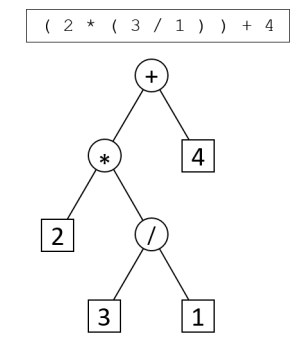
\includegraphics[width=0.25\paperwidth]{C:/Users/Admin/Desktop/Github/question_bank/LyX/static/img/9597-YIJC-2019-P1-Q3-2}
\par\end{center}

The following pseudocode (available in \texttt{PSEUDOCODE\_TASK\_3\_3.TXT})
can be used to add a node to the expression tree. 

\begin{minipage}[t]{0.88\columnwidth}%
\texttt{PROCEDURE Insert(NewToken)}

\texttt{\qquad{}IF NextFreeChild = -1 THEN // check if tree is full }

\texttt{\qquad{}\qquad{}RETURN 'Tree is Full'}

\texttt{\qquad{}// tree is not full, safe to insert new token }

\texttt{\qquad{}IF NextFreeChild = 0 THEN // inserting into empty
Tree }

\texttt{\qquad{}\qquad{}Tree{[}Root{]}.DataValue NewToken }

\texttt{\qquad{}\qquad{}NextFreeChild }

\texttt{\qquad{}\qquad{}Tree{[}Root{]}.LeftChild Tree{[}Root{]}.LeftChild
-1}

\texttt{\qquad{}ELSE }

\texttt{\qquad{}\qquad{}// inserting into tree with existing }

\texttt{\qquad{}\qquad{}// starting with Root }

\texttt{\qquad{}\qquad{}Current 0 // index of the current node }

\texttt{\qquad{}\qquad{}Previous -1 // index of previous node }

\texttt{\qquad{}\qquad{}NewNode Tree{[}NextFreeChild{]} // declare
new node }

\texttt{\qquad{}\qquad{}NewNode.DataValue NewToken }

\texttt{\qquad{}\qquad{}\qquad{}// Finding the node at which the
NewNode can be inserted }

\texttt{\qquad{}\qquad{}\qquad{}WHILE Current <> -1 THEN }

\texttt{\qquad{}\qquad{}\qquad{}\qquad{}CurrNode Tree{[}Current{]} }

\texttt{\qquad{}\qquad{}\qquad{}IF IsOperator(CurrNode.DataValue)
THEN }

\texttt{\qquad{}\qquad{}\qquad{}// check if CurrNode contains an
operator }

\texttt{\qquad{}\qquad{}\qquad{}\qquad{}IF CurrNode.LeftChild
= -1 THEN }

\texttt{\qquad{}\qquad{}\qquad{}\qquad{}// if LeftChild is empty,
insert here }

\texttt{\qquad{}\qquad{}\qquad{}\qquad{}\qquad{}CurrNode.LeftChild
NextFreeChild }

\texttt{\qquad{}\qquad{}\qquad{}\qquad{}\qquad{}NextFreeChild
NewNode.LeftChild }

\texttt{\qquad{}\qquad{}\qquad{}\qquad{}\qquad{}NewNode.LeftChild
-1 }

\texttt{\qquad{}\qquad{}\qquad{}\qquad{}\qquad{}Current -1}

\texttt{\qquad{}\qquad{}\qquad{}\qquad{}ELIF CurrNode.RightChild
= -1 THEN}

\texttt{\qquad{}\qquad{}\qquad{}\qquad{}\qquad{}// if RightChild
is empty, insert here }

\texttt{\qquad{}\qquad{}\qquad{}\qquad{}\qquad{}CurrNode.RightChild }

\texttt{\qquad{}\qquad{}\qquad{}\qquad{}\qquad{}NextFreeChild
NextFreeChild \textleftarrow{} NewNode.LeftChild }

\texttt{\qquad{}\qquad{}\qquad{}\qquad{}\qquad{}NewNode.LeftChild
-1}

\texttt{\qquad{}\qquad{}\qquad{}\qquad{}\qquad{}Current -1 }

\texttt{\qquad{}\qquad{}\qquad{}\qquad{}ELIF IsOperator(Tree{[}CurrNode.LeftChild{]}.DataValue)
THEN }

\texttt{\qquad{}\qquad{}\qquad{}\qquad{}\qquad{}// if LeftChild
is an operator, }

\texttt{\qquad{}\qquad{}\qquad{}\qquad{}\qquad{}// traverse leftchild
subtree }

\texttt{\qquad{}\qquad{}\qquad{}\qquad{}\qquad{}Previous Current }

\texttt{\qquad{}\qquad{}\qquad{}\qquad{}\qquad{}Current CurrNode.LeftChild}

\texttt{\qquad{}\qquad{}\qquad{}\qquad{}\qquad{}Fringe.APPEND(Previous)}

\texttt{\qquad{}\qquad{}\qquad{}\qquad{}ELIF IsOperator(Tree{[}CurrNode.RightChild{]}.DataValue)THEN }

\texttt{\qquad{}\qquad{}\qquad{}\qquad{}\qquad{}// if RightChild
is an operator, }

\texttt{\qquad{}\qquad{}\qquad{}\qquad{}\qquad{}// traverse rightchild
subtree }

\texttt{\qquad{}\qquad{}\qquad{}\qquad{}\qquad{}Previous Current}

\texttt{\qquad{}\qquad{}\qquad{}\qquad{}\qquad{}Current CurrNode.RightChild }

\texttt{\qquad{}\qquad{}\qquad{}\qquad{}\qquad{}Fringe.APPEND(Previous) }

\texttt{\qquad{}\qquad{}\qquad{}\qquad{}ELSE // traverse right
subtree }

\texttt{\qquad{}\qquad{}\qquad{}\qquad{}\qquad{}Previous Fringe.POP(-1) }

\texttt{\qquad{}\qquad{}\qquad{}\qquad{}\qquad{}Current Tree{[}Previous{]}.RightChild}

\texttt{\qquad{}\qquad{}\qquad{}\qquad{}ENDIF }

\texttt{\qquad{}\qquad{}\qquad{}ELSE // no place to insert}

\texttt{\qquad{}\qquad{}\qquad{}\qquad{}RETURN \textquotedbl Cannot
be inserted\textquotedbl{} }

\texttt{\qquad{}\qquad{}\qquad{}ENDIF }

\texttt{\qquad{}\qquad{}ENDWHILE}

\texttt{\qquad{}ENDIF}

\texttt{ENDPROCEDURE}%
\end{minipage}

\subsection*{Task 3.3 }

Write a code to implement the \texttt{Insert} method for the \texttt{ExpressionTree}
class from this pseudocode.

You may use the text file \texttt{PSEUDOCODE\_TASK\_3\_3.TXT} as a
basis for writing your code.

\subsection*{Evidence 3.3 }

Your program code for Task 3.3. \hfill{}{[}7{]}

\subsection*{Task 3.4: }

Write a code for the \texttt{Display} method for the \texttt{ExpressionTree}
class which displays the contents of \texttt{Tree} in index order. 

\subsection*{Evidence 3.4 }

Your program code for Task 3.4. \hfill{} {[}4{]}

\subsection*{Task 3.5 }

Write a sequence of program statements to: 
\begin{itemize}
\item create an expression tree
\item add the data items based on the sequence of commands given 
\item display the array contents 
\end{itemize}

\subsection*{Evidence 3.5 }

Your program code for Task 3.5. \hfill{}{[}3{]}

\subsection*{Evidence 3.6 }

Screenshot showing the output from running the program in Task 3.5.
\hfill{}{[}1{]}

\subsection*{Task 3.6 }

The infix notation can be obtained by performing an in-order traversal
in the expression tree. 

Write a code for the \texttt{infix} method for the \texttt{ExpressionTree}
class to generate the infix notation for a complete expression tree. 

\subsection*{Evidence 3.7 }

Your program code for Task 3.6. \hfill{} {[}6{]}

\subsection*{Evidence 3.8 }

Screenshot showing the output from running the program in Task 3.6.
\hfill{} {[}1{]}

\subsection*{Task 3.7 }

Write a code for the \texttt{calculate} method to evaluate and return
the numerical answer for the expression, rounded off to 2 decimal
places. 

\subsection*{Evidence 3.9 }

Your program code for Task 3.7. \hfill{}{[}3{]}

\subsection*{Evidence 3.10 }

Screenshot showing the output from running the program in Task 3.7.
\hfill{}{[}1{]}

 \newpage 

\item \textbf{{[}YIJC/PRELIM/9597/2019/P1/Q4{]} }

Minesweeper is a type of single-player puzzle game in which the player
continuously selects a cell in a square grid. Each cell contains either
a bomb or a value showing the number of bombs in the neighbouring
cell. (Neighbouring cells are those adjacent horizontally, vertically
or diagonally.)

If the player selects a cell that is a bomb, it \textquoteleft explodes\textquoteright{}
and he loses the game. The number of cells the player has selected
without exploding a bomb will be the player\textquoteright s score.

You are required to write a program code to generate a minesweeper
grid, randomly position the bombs and populate all the other cells
with the values indicating the number of bombs in the neighbouring
cells. Without revealing the minesweeper grid to the player, the program
should prompt the player to select the cells one by one. His score
will be the number of cells opened before hitting a bomb. 
\noindent \begin{center}
\begin{minipage}[t]{0.25\columnwidth}%
\texttt{X 2 1 1 }

\texttt{1 3 X 2 }

\texttt{0 2 X 3 }

\texttt{0 1 2 X }%
\end{minipage}
\par\end{center}

\subsection*{Task 4.1: }

Write a program code to generate and display an empty square grid
of size $n$, ie $n$ rows by $n$ columns. The minesweeper grid for
$n=5$ is as shown below: 
\noindent \begin{center}
\begin{minipage}[t]{0.25\columnwidth}%
\texttt{0 0 0 0 0 }

\texttt{0 0 0 0 0 }

\texttt{0 0 0 0 0 }

\texttt{0 0 0 0 0}

\texttt{0 0 0 0 0 }%
\end{minipage}
\par\end{center}

Your code should use a suitable data structure and fixed loop(s) to
display the grid.

\subsection*{Evidence 4.1: }

Your program code and screenshot of an empty grid of size 5.\hfill{}
{[}3{]}


\subsection*{Task 4.2: }

Write a program code to randomly place a bomb, represented by \textquotedbl X\textquotedbl ,
within the grid. Populate all the neighbouring cells by increasing
their values to 1 to indicate the presence of this one bomb in the
neighbourhood. 

\subsection*{Evidence 4.2: }

Your program code and two different screenshots of the grid ($n=5$).
\hfill{}{[}5{]}

\subsection*{Task 4.3: }

Modify the code written in Task 4.2 to randomly place two bombs within
the grid. Populate all the neighbouring cells with the correct values
to indicate the presence of the bombs in the neighbourhood. 

\subsection*{Evidence 4.3: }

Your program code and the screenshot of the grid ($n=5$) with 2 bombs.\hfill{}
{[}4{]}

\subsection*{Task 4.4: }

Modify the code written in Task 4.3 to generate $k$ numbers of bombs
within a grid of size $n$ and correctly display all the values in
the neighbouring cells surrounding the bombs. 

\subsection*{Evidence 4.4: }

Your program code and the screenshots of the minesweeper grids for
the following levels of difficulty. 
\begin{itemize}
\item Beginner (grid size $n=5$; no. of bombs $k=3$)
\item Intermediate (grid size $n=6$; no. of bombs $k=8$)
\item Expert (grid size $n=8$; no. of bombs $k=20$) {[}8{]}
\end{itemize}

\subsection*{Task 4.5: }

Write a program code to play the minesweeper game. Your code will:
\begin{itemize}
\item prompt the player to select the level of difficulty
\item generate the Minesweeper grid 
\item display a \textquotedblleft blank\textquotedblright{} grid with \textquoteleft -\textquoteright{}
for each of the cell prompt the player to input the coordinates of
a cell he wishes to open 
\begin{itemize}
\item If the opened cell is a bomb (\textquotedblleft X\textquotedblright ),
declare \textquotedblleft Game Over!\textquotedblright , show the
grid and display the player\textquoteright s score.
\item If the opened cell is not a bomb, show the updated grid with the opened
cell, increase the player\textquoteright s score by 1 and continue
with the game.
\end{itemize}
\item declare \textquotedblleft You have Won!\textquotedblright{} when the
player has opened all the possible cells and display the player\textquoteright s
score. 

{[}Sample screenshot of a typical game{]}: 

\noindent %
\begin{minipage}[t]{0.5\columnwidth}%
\texttt{Enter your cell you want to open:}

\texttt{X (1 to 5) : 2}

\texttt{Y (1 to 5) : 3}

\texttt{\_ \_ \_ \_ \_}

\texttt{\_ \_ 1 \_ \_}

\texttt{0 \_ \_ \_ \_}

\texttt{\_ \_ 1 \_ \_}

\texttt{\_ \_ \_ \_ \_}

\texttt{Your score is : 3}%
\end{minipage}%
\begin{minipage}[t]{0.5\columnwidth}%
\texttt{Enter your cell you want to open:}

\texttt{X (1 to 5) : 2}

\texttt{Y (1 to 5) : 4}

\texttt{X 1 1 1 1}

\texttt{1 1 1 X 1}

\texttt{0 0 1 1 1}

\texttt{0 1 1 1 0}

\texttt{0 1 X 1 0}

\texttt{Game over! You've hit the bomb at : (2,4).}

\texttt{Your score is : 3}

\texttt{Do you want to try again?}%
\end{minipage}
\end{itemize}

\subsection*{Evidence 4.5:}

Your program code and a screenshot of a game. \hfill{}{[}10{]}

 \newpage 

\item \textbf{{[}ACJC/PRELIM/9569/2021/P1/Q1{]} }

A food delivery app offers promotions to customers based on their
usage pattern. 

First time customers would receive a \$5 discount on their first purchase.
If a customer has spent at least \$1000 on the app in the last 3 months,
the app would upgrade the customer to Gold status and offer 10\% discount
on all orders. 

Gold status customers who have been inactive for 1 month would be
offered an additional 5\% discount on top of the existing 10\% discount.
Customers who have made their first purchase and have been inactive
for 1 month would receive a \$5 discount instead. 
\begin{enumerate}
\item Create a decision table to show these conditions and actions. \hfill{}{[}4{]}
\item Simplify your decision table by removing redundancies from the decision
table. \hfill{}{[}1{]}
\end{enumerate}

 \newpage 

\item \textbf{{[}ACJC/PRELIM/9569/2021/P1/Q2{]} }

The recursive function \texttt{Binomial} has two parameters, \texttt{N}
and \texttt{R}.

\noindent %
\noindent\begin{minipage}[t]{1\columnwidth}%
\texttt{01\qquad{}FUNCTION Binomial(N, R : INTEGERS) RETURNS INTEGER }

\texttt{02\qquad{}\qquad{}IF R = 0 OR R = N }

\texttt{03\qquad{}\qquad{}\qquad{}THEN }

\texttt{04\qquad{}\qquad{}\qquad{}\qquad{}Answer \textleftarrow{}
1 }

\texttt{05\qquad{}\qquad{}\qquad{}ELSE }

\texttt{06\qquad{}\qquad{}\qquad{}\qquad{}Answer \textleftarrow{}
Binomial(N \textendash{} 1, R) + Binomial(N \textendash{} 1, R \textendash{}
1) }

\texttt{07\qquad{}\qquad{}ENDIF }

\texttt{08\qquad{}\qquad{}RETURN Answer }

\texttt{09\qquad{}ENDFUNCTION}%
\end{minipage}
\begin{enumerate}
\item State what is meant by a recursive function, and identify the line
number that makes \texttt{Binomial} recursive. \hfill{}{[}2{]}
\item An example of a trace tree diagram showing the recursive function
call \texttt{Binomial(3,1)} is shown.
\begin{center}
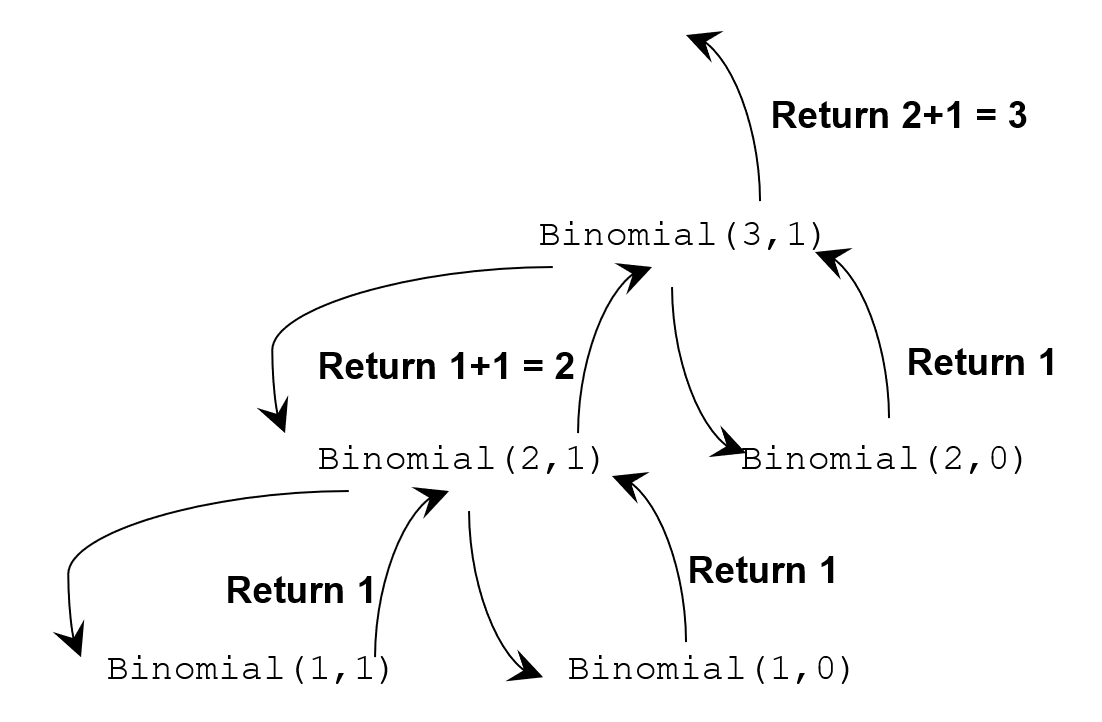
\includegraphics[width=0.5\paperwidth]{C:/Users/Admin/Desktop/Github/question_bank/LyX/static/img/9569-ACJC-2020-P1-Q2}
\par\end{center}

\end{enumerate}
Use the above example to create a trace tree diagram for the recursive
function call \texttt{Binomial(3,2)}. \hfill{}{[}4{]}
\begin{enumerate}
\item[(c)] Give values of N and R which would cause the function to enter infinite
recursion. \hfill{}{[}2{]}
\end{enumerate}

 \newpage 

\item \textbf{{[}ACJC/PRELIM/9569/2021/P1/Q3{]} }

The function \texttt{Evaluate} is designed to evaluate a polynomial
at a given value of $x$. The polynomial is stored as a queue of coefficients
in descending powers of x.

For example, the polynomial $5x^{3}-2x^{2}+3x-1$ is given as the
queue $[5,\lyxmathsym{\textendash}2,3,\lyxmathsym{\textendash}1]$,
where 5 is at the head of the queue.

\noindent %
\noindent\begin{minipage}[t]{1\columnwidth}%
\texttt{01\qquad{}FUNCTION Evaluate(X : INTEGER, Coeffs : QUEUE)
RETURNS INTEGER }

\texttt{02\qquad{}\qquad{}Answer \textleftarrow{} 0 }

\texttt{03\qquad{}\qquad{}REPEAT }

\texttt{04\qquad{}\qquad{}\qquad{}Answer \textleftarrow{} Answer
+ DEQUEUE Coeffs }

\texttt{05\qquad{}\qquad{}\qquad{}Answer \textleftarrow{} Answer
{*} X }

\texttt{06\qquad{}\qquad{}UNTIL Coeffs IS EMPTY }

\texttt{07\qquad{}\qquad{}RETURN Answer }

\texttt{08\qquad{}ENDFUNCTION}%
\end{minipage}
\begin{enumerate}
\item Draw a trace table to determine the output of the function \texttt{Evaluate}
for \texttt{X = 2} and \texttt{Coeffs = {[}5, \textendash 2, 3, \textendash 1{]}},
as described above. \hfill{}{[}4{]}
\item Describe the error in the function \texttt{Evaluate} as it is currently
written. \hfill{}{[}1{]}
\item Rewrite the pseudo-code above so that \texttt{Evaluate} returns the
correct value of the polynomial at a given value of \texttt{x}. \hfill{}{[}4{]}
\end{enumerate}

 \newpage 

\item \textbf{{[}ACJC/PRELIM/9569/2021/P1/Q4{]} }

During Home-Based Learning, many lessons were carried out over the
Internet.
\begin{enumerate}
\item For lessons carried out by video conferencing, tools by external companies
such as Zoom or Google Meet were used.

Give one example of an ethical consideration companies such as Zoom
or Google should take into account in this situation. \hfill{}{[}1{]}
\item Many lesson resources and homework submissions were carried out via
file uploads. Describe how a file can be uploaded from a student\textquoteright s
computer to a cloud drive by packet switching.\hfill{} {[}4{]}
\item For a Mother Tongue lesson, a teacher created a webpage in a non-English
language. Some students who accessed the webpage saw random characters
instead of the content intended by the teacher.
\begin{enumerate}
\item Describe the relevance of communications protocols in this context.
\hfill{}{[}2{]}
\item Describe how Unicode might address some of these problems.\hfill{}
{[}1{]}
\end{enumerate}
\end{enumerate}

 \newpage 

\item \textbf{{[}ACJC/PRELIM/9569/2021/P1/Q5{]} }

A printing shop offers printing services to its customers. When a
printing order is sent to the shop, the following information is recorded
down:
\begin{itemize}
\item Date of order 
\item Name of customer 
\item Number of copies 
\item Colour, or black and white, printing 
\item Whether express printing is required
\end{itemize}
The printing shop accepts three types of orders, leaflets, books and
posters.

Customers printing leaflets or books need to indicate if they require
single side or double side printing.

In addition, for books, the type of cover (hard cover or soft cover)
would need to be recorded. 

Leaflets and books are available in three sizes (A3, A4 or A5), while
posters are only available in a fixed size of A2.

For poster printing, customers have a choice of either glossy or matte
finishing.

The total charge to user is determined by the specifications of the
order and the formula is unique for each type of order.

This system is to be implemented using object-oriented programming
(OOP).
\begin{enumerate}
\item Draw a class diagram, showing:
\begin{itemize}
\item Any derived classes and inheritance from the base class 
\item The properties needed in the base, and any derived classes 
\item Suitable methods to support the system with at least one getter and
setter
\end{itemize}
The base class is \texttt{BASIC\_ORDER}. \hfill{}{[}8{]}
\item Explain the purpose of inheritance in object-oriented programing.
\hfill{}{[}2{]}
\end{enumerate}

 \newpage 

\item \textbf{{[}ACJC/PRELIM/9569/2021/P1/Q6{]} }

In a computer game, players\textquoteright{} names and scores are
stored in a binary search tree, in increasing order of score.

The binary search tree has its data inserted in the following order:

Ryan 18 

Bella 25 

Joshua 27 

Shane 20 

Jasmine 17 

Alexis 21 

Leslie 15
\begin{enumerate}
\item Draw the binary search tree. \hfill{}{[}4{]}
\item The binary search tree is implemented using the two dimensional array
shown below. Copy and fill in the entries in the array.
\noindent \begin{center}
\begin{tabular}{|c|c|c|c|c|}
\hline 
Index & Name & Score & Left Pointer & Right Pointer\tabularnewline
\hline 
0 &  &  &  & \tabularnewline
\hline 
1 &  &  &  & \tabularnewline
\hline 
2 &  &  &  & \tabularnewline
\hline 
3 &  &  &  & \tabularnewline
\hline 
4 &  &  &  & \tabularnewline
\hline 
5 &  &  &  & \tabularnewline
\hline 
6 &  &  &  & \tabularnewline
\hline 
\end{tabular}
\par\end{center}

\hfill{}{[}5{]}
\item To delete a node from a binary tree, the following cases are considered:
\noindent \begin{center}
\begin{tabular}{|l|l|}
\hline 
Case & Action\tabularnewline
\hline 
Node has no children & - Node is removed from tree\tabularnewline
\hline 
Node has one child & - Node is replaced with its child\tabularnewline
\hline 
\multirow{4}{*}{Node has two children} & - Call the node to be deleted $D$. Do not delete$D$\tabularnewline
\cline{2-2} 
 & - Look for the node $E$ that comes after $D$ in an in-order traversal\tabularnewline
\cline{2-2} 
 & - Copy the data $E$ into $D$.\tabularnewline
\cline{2-2} 
 & - Delete $E$ using one of the previous two cases.\tabularnewline
\hline 
\end{tabular}
\par\end{center}

Draw the tree at each step after the following players are deleted,
one after another:
\begin{enumerate}
\item Joshua \hfill{}{[}1{]}
\item Jasmine\hfill{} {[}1{]}
\item Ryan \hfill{}{[}2{]}
\end{enumerate}
\item The program has a feature which allows the user to enter an integer.
The program then returns a list of players whose score is greater
than that integer. Describe how the program can create this list using
the binary search tree. \hfill{}{[}4{]}
\end{enumerate}

 \newpage 

\quad{} 
\item \textbf{{[}ACJC/PRELIM/9569/2021/P1/Q7{]} }
\begin{enumerate}
\item The following is the pseudocode for an in-place quicksort algorithm
for sorting in ascending order.

\noindent %
\noindent\begin{minipage}[t]{1\columnwidth}%
\texttt{01\qquad{}FUNCTION Partition(L, R : INTEGERS, MyList : LIST)
RETURNS INTEGER }

\texttt{02\qquad{}\qquad{}Pivot \textleftarrow{} MyList{[}R{]} }

\texttt{03\qquad{}\qquad{}i \textleftarrow{} L }

\texttt{04\qquad{}\qquad{}j \textleftarrow{} L }

\texttt{05\qquad{}\qquad{}REPEAT }

\texttt{06\qquad{}\qquad{}\qquad{}IF MyList{[}j{]} > Pivot }

\texttt{07\qquad{}\qquad{}\qquad{}\qquad{}THEN }

\texttt{08\qquad{}\qquad{}\qquad{}\qquad{}\qquad{}}\texttt{\textbf{A}}\texttt{ }

\texttt{09\qquad{}\qquad{}\qquad{}\qquad{}ELSE }

\texttt{10\qquad{}\qquad{}\qquad{}\qquad{}Temp \textleftarrow{}
MyList{[}j{]} 11 MyList{[}j{]} \textleftarrow{} MyList{[}i{]} }

\texttt{12\qquad{}\qquad{}\qquad{}\qquad{}}\texttt{\textbf{B}}\texttt{ }

\texttt{13\qquad{}\qquad{}\qquad{}ENDIF }

\texttt{14\qquad{}\qquad{}UNTIL j = R }

\texttt{15\qquad{}\qquad{}MyList{[}R{]} \textleftarrow{} MyList{[}i{]}
// swap elements with index i and R }

\texttt{16\qquad{}\qquad{}MyList{[}i{]} \textleftarrow{} Pivot }

\texttt{17\qquad{}\qquad{}}\texttt{\textbf{C}}\texttt{ }

\texttt{18\qquad{}ENDFUNCTION }

\texttt{19\qquad{}PROCEDURE Quicksort(L, R : INTEGERS, MyList : LIST) }

\texttt{20\qquad{}\qquad{}IF }\texttt{\textbf{D}}\texttt{ }

\texttt{21\qquad{}\qquad{}\qquad{}THEN }

\texttt{22\qquad{}\qquad{}\qquad{}\qquad{}PivotPos = Partition(R,
L, MyList) }

\texttt{23\qquad{}\qquad{}\qquad{}\qquad{}CALL Quicksort(L, PivotPos
- 1, MyList) }

\texttt{24\qquad{}\qquad{}\qquad{}\qquad{}}\texttt{\textbf{E}}\texttt{ }

\texttt{25\qquad{}\qquad{}ENDIF }

\texttt{26\qquad{}ENDPROCEDURE}%
\end{minipage}
\begin{enumerate}
\item Write pseudo-code to replace \texttt{\textbf{A}}, \texttt{\textbf{B}},
\texttt{\textbf{C}}, \texttt{\textbf{D}} and \texttt{\textbf{E}} in
the above algorithm. \hfill{}{[}5{]}
\item State the time complexity of the algorithm in the above pseudo-code.
\hfill{} {[}1{]}
\item State and explain when the worst case scenario (for running time)
for quicksort arises in the above algorithm. \hfill{}{[}3{]}
\item Another programmer suggested insertion sort would be more efficient
during the worst case scenario in (iii).

State and explain if insertion sort is indeed more efficient in this
instance. \hfill{}{[}2{]}
\end{enumerate}
\item A program needs to store an array of names and scores in a two dimensional
array and perform the following:
\begin{itemize}
\item Output the names and scores in alphabetical order. 
\item Check for the presence of a particular name
\end{itemize}
The data to be stored in the array is as follows:

Peter 68 

Mary 70 

Kelvin 48 

Casper 44 

Luther 76
\begin{enumerate}
\item Draw a flowchart to represent a linear search algorithm that returns
the score of a particular name. \hfill{} {[}4{]}
\item Instead of storing the data in an array, it is suggested that the
names could be stored in a hash table instead. 

With reference to the requirements of the program, suggest one advantage
and one disadvantage of storing the names in a hash table instead
of an array. \hfill{} {[}2{]}
\item (iii) An array can be used to create the hash table data structure.
Describe the process of inserting the above data into a hash table.
You may assume there will be no collisions. \hfill{} {[}3{]}
\end{enumerate}
\end{enumerate}

 \newpage 

\item \textbf{{[}ACJC/PRELIM/9569/2021/P1/Q8{]} }

A programmer is tasked to write a program to store the examination
scores of students in the entire school. For each student, the database
would need to store the following data: name, form class, subject
class, subject, score and subject teacher.
\begin{enumerate}
\item Suggest a suitable data type for each of the following fields: 
\begin{itemize}
\item Name 
\item Class 
\item Score \hfill{}{[}2{]}
\end{itemize}
\item The programmer is considering storing this data in either a relational
or non-relational database.
\begin{enumerate}
\item State three key differences between the two types of databases. \hfill{}{[}3{]}
\item State and explain which database system the programmer should choose.
\hfill{}{[}3{]}
\end{enumerate}
\end{enumerate}
A healthcare group would like to store patient data in a relational
database. When a patient visits the clinic, the clinic will record
the following information:
\begin{itemize}
\item Date and time of visit 
\item Name of attending doctor and his NRIC 
\item Patient name and NRIC number
\end{itemize}
After the doctor has attended to the patient, the patient would be
given a prescription. The prescription would record the medication
which the patient is supposed to take. Each prescription, which consists
of at least one medicine, would have its own unique identification
number. Each medicine would have a unique identification number, name
and price. 

The data is stored in a relational database with five tables: \texttt{Patient},
\texttt{Doctor}, \texttt{Appointment}, \texttt{Prescription} and \texttt{Medicine}.
\begin{enumerate}
\item[(c)]  Draw the Entity-Relationship (E-R) diagram to show the tables in
third normal form (3NF) and the relationships between them. \hfill{}{[}7{]}
\item[(d)]  A table description can be written as:

\texttt{TableName (Attribute1, Attribute2, Attribute3, \dots )}

The primary key is indicated by underlining one or more attributes.
Foreign keys are indicated by using a dashed underline.

Using the information provided, write table descriptions for the tables
you identified in part (c). \hfill{}{[}8{]}
\end{enumerate}

 \newpage 

\item \textbf{{[}ACJC/PRELIM/9569/2021/P2/Q1{]} }

A programmer is writing a program to implement a role-playing computer
game using Object-Oriented Programming (OOP).

The players have to collect food items. A food item has the following
attributes:
\begin{itemize}
\item \texttt{name : STRING }
\item \texttt{value : INTEGER}
\end{itemize}
and the following methods:
\begin{itemize}
\item \texttt{get\_name() }
\item \texttt{get\_value()}
\end{itemize}
A player takes on the role of a person. A person has the following
attributes:
\begin{itemize}
\item \texttt{name : STRING }
\item \texttt{health : INTEGER} which is initialised at a value of \texttt{100}
\item \texttt{strength : INTEGER} which is initialised at a value of \texttt{100}
\end{itemize}
and the following methods:
\begin{itemize}
\item \texttt{get\_name() }
\item \texttt{get\_health() }
\item \texttt{get\_strength() }
\item \texttt{eat(food)} adds the value of the food to the strength. The
code should display the player\textquoteright s new strength. 
\item \texttt{attack(opponent)}
\end{itemize}
For the \texttt{attack} method, \texttt{opponent} is another person.
\begin{itemize}
\item A random integer \texttt{r} between \texttt{1} and \texttt{10} (inclusive)
is generated. 
\item If the player\textquoteright s \texttt{strength} is less than \texttt{r},
then the player does not have enough strength to attack and there
is no change to \texttt{opponent}\textquoteright s \texttt{health}. 
\item If the player\textquoteright s \texttt{strength} is at least \texttt{r},
then the attack is successful and \texttt{opponent}\textquoteright s
\texttt{health} is decreased by \texttt{r}. 
\begin{itemize}
\item If opponent\textquoteright s health is now negative, then opponent
has been defeated. 
\end{itemize}
\item The player\textquoteright s \texttt{strength} is decreased by r.
\end{itemize}
There are two subclasses of the \texttt{Person} class -- \texttt{Healer}
and the \texttt{Warrior}.

Healer has one additional method:
\begin{itemize}
\item \texttt{heal(patient)}
\end{itemize}
\quad{}

For the \texttt{heal} method, \texttt{patient} is another person.
\begin{itemize}
\item A random integer \texttt{r} between \texttt{1} and \texttt{10} (inclusive)
is generated. 
\item If the player\textquoteright s \texttt{strength} is less than \texttt{r},
then the player does not have enough strength to heal and there is
no change to \texttt{patient}\textquoteright s \texttt{health}. 
\item If the player\textquoteright s \texttt{strength} is at least \texttt{r},
then the healing is successful and \texttt{patient}\textquoteright s
\texttt{health} is increased by \texttt{r}, up to a maximum of \texttt{100}.
\end{itemize}
\texttt{Warrior}\textquoteright s \texttt{attack} method is twice
as effective, meaning that if the player has enough strength to attack,
\texttt{opponent}\textquoteright s \texttt{health} is decreased by
\texttt{2{*}r}, while the player\textquoteright s \texttt{strength}
is decreased by \texttt{r}.

\subsubsection*{Task 1.1}

Write program code to define the class \texttt{Food}. \hfill{}{[}3{]}

\subsubsection*{Task 1.2}

Write program code to define the class \texttt{Person}.

The code should display appropriate messages about the outcome of
\texttt{attack}, including the new value of opponent\textquoteright s
\texttt{health}. \hfill{}{[}10{]}

\subsubsection*{Task 1.3}

Use appropriate inheritance to write program code to define the class
\texttt{Healer}.

The code should display appropriate messages about the outcome of
\texttt{heal}, including the new value of \texttt{patient}\textquoteright s
\texttt{health}. \hfill{}{[}4{]}

\subsubsection*{Task 1.4}

Use appropriate inheritance and polymorphism to write program code
to define the class \texttt{Warrior}. \hfill{}{[}2{]}

Test your code with the following steps in order:
\begin{itemize}
\item Create a \texttt{Food} item with name \texttt{'Cheese'} and value
\texttt{10}. 
\item Create a \texttt{Warrior} with \texttt{name} \texttt{'Sam'}. 
\item Create a \texttt{Healer} with name \texttt{'Alex'}. 
\item Create a \texttt{Person} with name \texttt{'Jan'}. 
\item \texttt{'Jan'} attacks \texttt{'Sam'}. 
\item \texttt{'Sam'} attacks \texttt{'Jan'}. 
\item \texttt{'Alex'} heals \texttt{'Jan'}. 
\item \texttt{'Sam'} eats \texttt{'Cheese'}.
\end{itemize}
Download your program code and output for Task 1 as \texttt{TASK1\_<your
name>\_<centre number>\_<index number>.ipynb} \hfill{}{[}3{]}

 \newpage 

\item \textbf{{[}ACJC/PRELIM/9569/2021/P2/Q2{]} }

An $\mathtt{n\times n}$ chessboard consists of an $\mathtt{n\times n}$
grid of small squares. For this task, the squares are numbered using
a coordinate system as a tuple of two integers. The first integer
is the column number, starting from \texttt{1} at the left, and the
second integer is the row number, starting from \texttt{1} at the
bottom.

A chess knight is a piece that occupies a square, and can then move
to another square according to one of the following rules:
\begin{itemize}
\item moving two squares horizontally and then one square vertically in
either direction, or 
\item moving two squares vertically and then one square horizontally in
either direction.
\end{itemize}
See the diagram below for examples.
\begin{center}
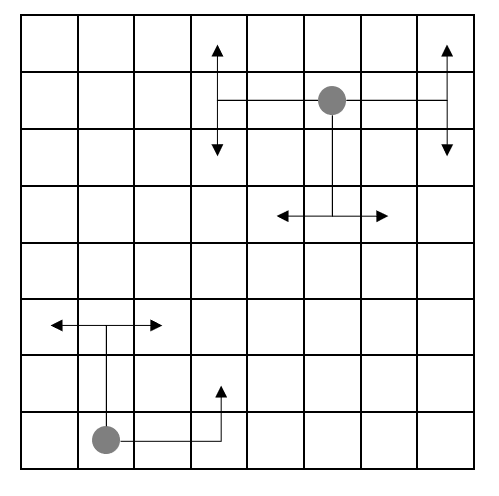
\includegraphics[width=0.5\paperwidth]{C:/Users/Admin/Desktop/Github/question_bank/LyX/static/img/9569-ACJC-2020-P2-Q2}
\par\end{center}

The knight at \texttt{(2,1)} can move to \texttt{(1,3)}, \texttt{(3,3)}
or \texttt{(4,2)}. 

The knight at \texttt{(6,7)} can move to \texttt{(4,6)}, \texttt{(4,8)},
\texttt{(5,5)}, \texttt{(7,5)}, \texttt{(8,6)} or \texttt{(8,8)}.

Only the starting and ending squares of the knight\textquoteright s
move are counted as being visited by the knight, and not the squares
that the knight passes over while moving.

A knight\textquoteright s tour is a sequence of moves that a chess
knight makes on a chessboard, so that it visits every square of the
chessboard exactly once. It does not need to return to its starting
square.

\subsubsection*{Task 2.1}

For a given value of \texttt{n} and a list of squares, write program
code to determine if the list is a knight\textquoteright s tour of
an $\mathtt{n\times n}$ chessboard.

Test your code using the values\texttt{ $\mathtt{n=7}$} and the list
of squares given in the files: 
\begin{itemize}
\item \texttt{TASK2TOUR.txt}, which is a valid tour; 
\item \texttt{TASK2NOTOUR.txt}, which is not a valid tour. \hfill{}{[}10{]}
\end{itemize}
An algorithm to generate a knight\textquoteright s tour needs to keep
track of the squares already visited, so that the knight does not
visit them a second time during the tour.

\subsubsection*{Task 2.2}

Suppose the knight is currently on square square, and a list of squares
already visited by the knight is given in \texttt{lis}.

Write a function \texttt{available(square,lis)} that returns a list
of squares which the knight can visit on its next move from \texttt{square},
and are not currently in \texttt{lis}. These are the squares available
to the knight as it tries to complete the tour.

The output should be given in lexicographic order, that is, with the
column numbers in ascending order, and, among the squares with the
same column number, with the row numbers in ascending order. \hfill{}{[}6{]}

\subsubsection*{Task 2.3}

The knight starts at \texttt{(1,1)}, the bottom left square, of an
$8\mathtt{\times}8$ chessboard.

From each square, the knight moves to the available square from which
it has the smallest number of available squares after that. If there
is a tie, the square which comes first in lexicographic order is chosen.

Write program code to generate the knight\textquoteright s tour as
a list of squares in the order they are visited.

Download your program code and output for Task 2 as \texttt{TASK2\_<your
name>\_<centre number>\_<index number>.ipynb}\hfill{} {[}9{]}

 \newpage 

\item \textbf{{[}ACJC/PRELIM/9569/2021/P2/Q3{]} }

A text file \texttt{INVENTORY.txt} contains the inventory data for
a certain electronics store. Each line in the file contains tab-delimited
data that shows the product name, product type, purchase price, selling
price and quantity available.

Each line is in the format

\texttt{Name\textbackslash tType\textbackslash tPurchase\_Price\textbackslash tSelling\_Price\textbackslash tQuantity}

where \texttt{\textbackslash t} represents the tab character.

\subsection*{Task 3.1 }

Write program code to:
\begin{itemize}
\item Read the inventory data from the text file; 
\item Find the average selling price of products belonging to the \texttt{Laptop}
product type and display this value; 
\item Count the number of products in each product type and store it in
appropriate data structure called \texttt{TypeCount}; 
\item Display the product type with the greatest number of products. If
there is a tie, display all of the product types with the greatest
number of products.
\end{itemize}
Download your program code and output for Task 3.1 as 

\texttt{TASK3\_1\_<your name>\_<centre number>\_<index number>.ipynb}
\hfill{}{[}6{]}

\subsection*{Task 3.2 }

The profit margin of each product can be calculated by the following
equation:
\noindent \begin{center}
Profit margin = selling price -- purchase price.
\par\end{center}

Write program code to:
\begin{itemize}
\item Calculate and display the total profit the store could make if all
products are sold; 
\item Sort the inventory data using a Merge sort algorithm in descending
order of profit margin; 
\item Display the sorted inventory data in the format given below.
\noindent \begin{center}
\texttt{}%
\begin{tabular}{lll}
\texttt{Product } & \texttt{Product Type } & \texttt{Profit Margin }\tabularnewline
\texttt{ThinkingPad 14} & \texttt{Computer } & \texttt{300 }\tabularnewline
\texttt{Bapple 8 } & \texttt{Phone } & \texttt{450}\tabularnewline
\end{tabular}
\par\end{center}

\end{itemize}
Download your program code and output for Task 3.2 as 

\texttt{TASK3\_2\_<your name>\_<centre number>\_<index number>.ipynb}\hfill{}
{[}9{]}

\subsection*{Task 3.3}

A store manager decided to make some changes to \texttt{INVENTORY.txt}
and saved it as \texttt{INVENTORY\_SERIAL.txt}. Each line in the updated
file contains tab-delimited data that shows the serial number, product
name, product type, purchase price, selling price and quantity available.

Each line is in the format:

\texttt{Serial\_No\textbackslash tName\textbackslash tType\textbackslash tPurchase\_Price\textbackslash tSelling\_Price\textbackslash tQuantity}

where \texttt{\textbackslash t} represents the tab character.

Write program code to insert the data from \texttt{INVENTORY\_SERIAL.txt}
into a NoSQL database \texttt{OUTLETS} under the collection \texttt{GEM}.

Download your program code for Task 3.3 as 

\texttt{TASK3\_3\_<your name>\_<centre number>\_<index number>.py}
\hfill{}{[}5{]}

\subsection*{Task 3.4}

The database administrator wants to validate that the store manager
did not make any errors when he edited the text file. Write program
code to check that the database conforms to the below specifications:
\begin{itemize}
\item \texttt{Serial\_No} consists of one digit followed by two letters,
followed by one digit (e.g. \texttt{1AB7}); 
\item \texttt{Name} consists of only letters, digits and spaces; 
\item \texttt{Quantity} is a positive integer. 
\end{itemize}
Any document that has an error should be removed from the database.
You may assume data fields not specified above are error free. Display
the documents that were removed.

Download your program code for Task 3.4 as 

\texttt{TASK3\_4\_<your name>\_<centre number>\_<index number>.py}
\hfill{}{[}5{]}

 \newpage 

\item \textbf{{[}ACJC/PRELIM/9569/2021/P2/Q4{]} }

A company keeps records of the employees working for it. The following
are the information stored in the company\textquoteright s database:
\begin{itemize}
\item \texttt{Employee\_name} -- name of the employee 
\item \texttt{Employee\_ID} -- unique ID number allocated to each employee 
\item \texttt{Job\_type} -- type of job the employee is employed for (\texttt{'Sales'}
or \texttt{'Tech\_support}') 
\item \texttt{Date\_of\_employment} -- date the employee joined the company 
\item \texttt{Service\_status} -- whether the employee is still in service
(\texttt{'True'} means the employee is still in the company, \texttt{'False'}
means the employee has left the company) 
\end{itemize}
For sales employees, the following extra information is recorded:
\begin{itemize}
\item \texttt{Total\_sales} -- the amount of sales in dollars made by the
employee 
\end{itemize}
For tech support employees, the following extra information is recorded:
\begin{itemize}
\item \texttt{Bugs\_resolved} -- the total number of bugs the employee
has resolved 
\end{itemize}
The database is expected to be normalised and stored in three different
tables:

\texttt{Employee }

\texttt{Sales }

\texttt{Tech\_support}

\subsection*{Task 4.1}

Create an SQL file called \texttt{TASK4\_1\_<your name>\_<centre number>\_<index
number>.sql} to show the SQL code to create the database \texttt{records.db}
with the three tables. Primary keys and foreign keys should be defined
where appropriate.

Save your SQL code as 

\texttt{TASK4\_1\_<your name>\_<centre number>\_<index number>.sql}
\hfill{}{[}5{]}

\subsection*{Task 4.2 }

The files \texttt{SALES.txt} and \texttt{TECH\_SUPPORT.txt} contain
information regarding the sales and tech support employees respectively.
The information should be inserted into the database.

For \texttt{SALES.txt}, information is given in the following order: 

\texttt{Employee\_ID}, \texttt{Employee\_name}, \texttt{Date\_of\_Employment},
\texttt{Service\_status}, \texttt{Total\_Sales}

For \texttt{TECH\_SUPPORT.txt}, information is given in the following
order: 

\texttt{Employee\_ID}, \texttt{Employee\_name}, \texttt{Date\_of\_Employment},
\texttt{Service\_status}, \texttt{Bugs\_resolved}

Write a python program to insert all information from the two files
into the \texttt{records} database, \texttt{records.db}. Run the program.

Save your program code as 

\texttt{TASK4\_2\_<your name>\_<centre number>\_<index number>.py}\hfill{}
{[}5{]}

\subsection*{Task 4.3}

The company wants to filter the employees by \texttt{Service\_status}
and display the results in a web browser.

Write a Python program and the necessary files to create a web application
that:
\begin{itemize}
\item receives a \texttt{Service\_status} string from a HTML form, then
\item creates and returns a HTML document that enables the web browser to
display either
\begin{itemize}
\item an ordered list of employees that are still in service, or 
\item an ordered list of employees that are no longer in service,
\end{itemize}
depending on the \texttt{Service\_status} string entered by the user.
\end{itemize}
The list should be sorted in alphabetical order.

Save your Python program as 

\texttt{TASK4\_3\_<your name>\_<centre number>\_<index number>.py }

with any additional files / sub-folders as needed in a folder named 

\texttt{TASK4\_3\_<your name>\_<centre number>\_<index number>}

Run the web application. Save the output of the program when \texttt{'TRUE'}
is entered as the \texttt{Service\_status} as \texttt{TASK4\_3\_<your
name>\_<centre number>\_<index number>.html}. \hfill{}{[}12{]}

 \newpage 

\item \textbf{{[}DHS/PRELIM/9569/2020/P1/Q1{]} }

Given an array of numbers \texttt{A}, count the minimum number of
'bubble sort' swaps (swap between pair of consecutive items) needed
to sort the array in ascending order. 

For example, if \texttt{A = {[}3, 2, 1, 4{]}}, we need 3 'bubble sort'
swaps to sort A in ascending order i.e. 

\texttt{swap(3, 2)} to get \texttt{{[}}\texttt{\uline{2, 3}}\texttt{,
1, 4{]} }

\texttt{swap(3, 1)} to get \texttt{{[}2, }\texttt{\uline{1, 3}}\texttt{,
4{]}} 

\texttt{swap(1, 2)} to get \texttt{{[}}\texttt{\uline{1, 2}}\texttt{,
3, 4{]}} 
\begin{enumerate}
\item Devise an $O(n^{2})$ algorithm using bubble sort to count the number
of 'bubble sort' swaps. 
\item Devise an $O(n\log n)$ algorithm to count the number of 'bubble sort'
swaps. 
\end{enumerate}
You should also explain why each algorithm has its efficiency. \hfill{}{[}8{]}
\begin{enumerate}
\item[(c)] Would you expect insertion sort to perform better or worse than bubble
sort in (a)? Explain your answer with respect to the number of comparisons
needed using the above example.\hfill{} {[}5{]}
\item[(d)] Why is quick sort not a suitable algorithm in part (b)? Illustrate
your answer with a suitable example. \hfill{}{[}5{]}
\end{enumerate}

 \newpage 

\item \textbf{{[}DHS/PRELIM/9569/2020/P1/Q2{]} }

You have been tasked to use a suitable data structure to manage the
preliminary exam results of students in Dunman High School. Each student
is identified by its centre and index numbers, each of which is 4-digit.
For example, Lim Ah Seng's identification number is 30420188. A typical
range of students' identification numbers are from 30420001 to 30420450,
since each graduating cohort will have about 450 students. 

The preliminary examination details to be stored are as follows: 
\begin{itemize}
\item Subject code (4-digit) eg 9569 
\item Subject name eg H2 Computing 
\item Subject grade (1-character eg 'A') You may assume that each student
will have a valid subject grade in the range of {[}'A', 'B', 'C',
'D', 'E', 'S', 'U', 'T', '0'{]}, where 'T' stands for terminated and
'0' stands for absent. 
\end{itemize}
Using suitable examples, evaluate the pros and cons using each of
the following data structure to store the required information: 
\begin{enumerate}
\item dictionary 
\item hash table \hfill{}{[}12{]}
\end{enumerate}

 \newpage 

\item \textbf{{[}DHS/PRELIM/9569/2020/P1/Q3{]} }

The information in Question 2 will also be stored in a relational
database. 
\begin{enumerate}
\item Why is a relational database model more suitable than a NoSQL database
model for storing the required information? \hfill{}{[}3{]}
\item Draw an ER diagram for a normalised database design. \hfill{}{[}4{]}
\item Produce the specification for the tables. \hfill{}{[}5{]}
\item Using examples in this context, explain the significance of the following
terms: 
\begin{enumerate}
\item primary key \hfill{}{[}2{]}
\item foreign key \hfill{}{[}2{]}
\item 1NF\hfill{} {[}2{]}
\item 2NF\hfill{} {[}2{]}
\item 3NF \hfill{}{[}2{]}
\end{enumerate}
\item What is the relationship between the data structures in Question 2
and a relational database? \hfill{}{[}4{]}
\end{enumerate}

 \newpage 

\item \textbf{{[}DHS/PRELIM/9569/2020/P1/Q4{]} }

The following diagram shows the contents with some data inserted. 
\begin{enumerate}
\item State two possible insertion orders of data to this BST.\hfill{}
{[}2{]}
\item Generalise how data can be inserted to produce a balanced BST.\hfill{}
{[}3{]}
\item The BST is to be implemented using a 1D array T. Write pseudocode
to show how data can be represented in T with suitable initial values
for an empty BST. \hfill{}{[}4{]}
\item Devise a recursive algorithm to insert to this BST. \hfill{}{[}5{]}
\item Devise a recursive algorithm to check if T is a BST. \hfill{}{[}3{]}
\item Convert the recursive algorithm in part (e) to an iterative one using
a suitable data structure which you should name and justify. \hfill{}{[}5{]}
\item Devise an algorithm to output the items in T that are within a given
range {[}a, b{]} inclusive in ascending order.\hfill{} {[}4{]}
\item Devise an algorithm to output the contents of the leaves of T in descending
order.\hfill{} {[}4{]}
\item Despite its memory overhead, why is recursion often used in BSTs?
\hfill{}{[}3{]}
\item Why is recursion less often used in linked lists?\hfill{} {[}2{]}
\end{enumerate}

 \newpage 

\item \textbf{{[}DHS/PRELIM/9569/2020/P1/Q5{]} }

A student came up with the following Python program to implement a
linked list data structure:

\noindent %
\noindent\begin{minipage}[t]{1\columnwidth}%
\texttt{01\qquad{}class Node: }

\texttt{02\qquad{}\qquad{}def \_\_init\_\_(self, data): }

\texttt{03\qquad{}\qquad{}self.data = data }

\texttt{04\qquad{}\qquad{}self.link = None }

\texttt{05 }

\texttt{06\qquad{}def insert(data): }

\texttt{07\qquad{}\qquad{}global head }

\texttt{08\qquad{}\qquad{}if head == None: \# empty linked list }

\texttt{09\qquad{}\qquad{}\qquad{}head = Node(data) }

\texttt{10\qquad{}\qquad{}else: \# insert to front }

\texttt{11\qquad{}\qquad{}\qquad{}new\_node = Node(data) }

\texttt{12\qquad{}\qquad{}\qquad{}new\_node.link = head }

\texttt{13\qquad{}\qquad{}\qquad{}head = new\_node }

\texttt{14 }

\texttt{15\qquad{}\qquad{}def display(): }

\texttt{16\qquad{}\qquad{}\qquad{}global head }

\texttt{17\qquad{}\qquad{}\qquad{}curr = head }

\texttt{18\qquad{}\qquad{}\qquad{}while curr: }

\texttt{19\qquad{}\qquad{}\qquad{}\qquad{}print(curr.data) }

\texttt{20\qquad{}\qquad{}\qquad{}\qquad{}curr = curr.link }

\texttt{21 }

\texttt{22\qquad{}\# main }

\texttt{23\qquad{}head = None }

\texttt{24\qquad{}insert(\textquotedbl Ali\textquotedbl ) }

\texttt{25\qquad{}insert(\textquotedbl Tom\textquotedbl ) }

\texttt{26\qquad{}insert(\textquotedbl Mary\textquotedbl ) }

\texttt{27\qquad{}display() }%
\end{minipage}
\begin{enumerate}
\item What will be the output of line 27?\hfill{} {[}1{]}
\item Comment on the programming paradigms used and identify any potential
pitfalls in the above program.\hfill{}{[}5{]}
\item Why is OOP appropriate in the implementation of data structures such
as linked lists?\hfill{}{[}2{]}
\item The above program maintains an unordered linked list. Devise an algorithm
to insert to an ordered linked list.\hfill{}{[}5{]}
\item A linked list can be ordered or unordered. Draw a UML class diagram
to illustrate the concepts of encapsulation, inheritance and polymorphism.\hfill{}
{[}5{]}
\item Explain how polymorphism is applied to the \texttt{insert()} rather
than the \texttt{display()} method in this context.\hfill{} {[}3{]}
\end{enumerate}

 \newpage 

\item \textbf{{[}DHS/PRELIM/9569/2020/P1/Q6{]} }

On 14 September 2020, it was reported that GrabCar was fined S\$10,000
for a 4th user data privacy violation. The Personal Data Protection
Commission (PDPC) said the update risked the personal data of 21,541
drivers and passengers, including profile pictures, names and vehicle
plate numbers. 

GrabCar rolled back the app to the previous version within about 40
minutes and took other remedial action, PDPC said. 

On Aug 30, 2019, GrabCar notified the PDPC that profile data of 5,651
GrabHitch drivers was exposed to the risk of unauthorised access by
other GrabHitch drivers for a \textquotedbl short period of time
on the same day\textquotedbl{} through the Grab app. 

Grab's investigations traced the cause of the breach to a deployment
of an update to the app on the same day. The purpose of the update
was to address a potential vulnerability discovered within the Grab
app. 

In PDPC's findings, the application programming interface URL which
allowed GrabHitch drivers to access their data, had contained a \textquotedbl userID\textquotedbl{}
portion that could potentially be manipulated to allow access to other
drivers' data. According to GrabCar, there was no evidence that this
vulnerability was exploited. 

To fix the vulnerability, the update removed the \textquotedbl userID\textquotedbl{}
from the URL, which shortened it to a hard-coded \textquotedbl users/profile\textquotedbl .
However, it failed to take into account the URL-based caching mechanism
in the app, which was configured to refresh every 10 seconds. 

The mechanism served cached content in response to data requests,
so as to reduce the load of direct access to GrabCar's database. 

With the update, all URLs in the Grab app ended with \textquotedbl users/profile\textquotedbl .
Without the \textquotedbl userID\textquotedbl{} in the URL, which
directed data requests to the correct GrabHitch driver's accounts,
the caching mechanism could no longer differentiate between drivers. 

Thus, the mechanism provided the same data to all GrabHitch drivers
for 10 seconds before new data was retrieved from GrabCar's database
and cached for the next 10 seconds. 

PDPC said GrabCar did not put in place \textquotedbl sufficiently
robust processes\textquotedbl{} to manage changes to its IT system
that may put personal data it was processing at risk. 

\textquotedbl This was a particularly grave error given that this
is the second time the (GrabCar) is making a similar mistake, albeit
with respect to a different system,\textquotedbl{} he said.

In a statement in response to Reuters' query, Grab said: \textquotedbl To
prevent a recurrence, we have since introduced more robust processes,
especially pertaining to our IT environment testing, along with updated
governance procedures and an architecture review of our legacy application
and source codes.\textquotedbl{} 

In 2019, GrabCar was ordered to pay a financial penalty of S\$16,000
after it sent out more than 120,000 marketing emails to customers
containing the name and mobile phone number of another customer. 

The PDPC had found that GrabCar \textquotedblleft failed to make reasonable
security arrangements\textquotedblright{} to detect the errors in
their database when sending out the emails. 

Source: Reuters/CNA/lk 

Adapted from https://www.channelnewsasia.com/news/business/grab-car-hitch-pdpc-personal-data-risk-fin
e-13108144 
\begin{enumerate}
\item For each of the following, suggest two ways in which the data leaks
could have been exploited by a malicious hacker with reference to 
\begin{enumerate}
\item profile pictures, names and vehicle plate numbers of drivers and passengers\hfill{}
{[}2{]}
\item name and mobile phone number of customers \hfill{}{[}2{]}
\end{enumerate}
\item What could have caused 
\begin{enumerate}
\item the URL related data leak? 
\item the marketing emails related data leak? 
\item the repeated data leaks? 
\end{enumerate}
You should provide a balance of technical and human related reasons.
\hfill{}{[}6{]}
\item How can Grab ensure and assure PDPC that sufficiently robust processes
have been put in place? \hfill{}{[}3{]}
\end{enumerate}

 \newpage 

\item \textbf{{[}DHS/PRELIM/9569/2020/P2/Q1{]} }

On 28 June 2020, nearly 10,000 TraceTogether tokens were distributed
to vulnerable seniors. The TraceTogether token supplements the TraceTogether
mobile app by extending contact tracing to groups in the community
who do not have smart phones and those whose phones do not work well
with the TraceTogether app. 

The TraceTogether token is designed to capture proximity data based
on Bluetooth signals. Every five minutes, it scans to detect other
TraceTogether users on the token or the app. The more 'hits' between
two TraceTogether users, the more likely they are in close proximity
for an extended period of time. Proximity can be estimated by the
strength of the Bluetooth signal. The closer users are to one another,
the stronger the signal and vice versa. 

There are only four types of data contained in the token: 
\begin{itemize}
\item user's randomised ID 
\item randomised ID of any other user in proximity 
\item Bluetooth signal measured using RSSI{*} 
\item timestamp of the encounter. 
\end{itemize}
{*}Received Signal Strength Indicator (RSSI) is a measure of the power
level at the receiver. A more negative number indicates a device is
further away. For example, a value of -20 to -30 indicates a device
is close while a value of -120 indicates it is near the limit of detection. 

It is important to note that these IDs do not refer to NRIC number,
but randomised and anonymised IDs linked to a personal identifier
like a mobile number. Also, no data is extracted unless a user has
tested positive for COVID-19. From there, MOH has a special software
key that can unlock the device and reveal the data for use in contact
tracing. 

A senior is tested positive for COVID-19 and MOH needs to perform
contact tracing. With the user's permission, data from its TraceTogether
token is retrieved and extracted to the file \texttt{TOKEN.txt} and
has the following structure: 

\texttt{UserRandomisedID, OtherRandomisedID, RSSI, Timestamp} 

Timestamp is in the format YYYY-MM-DD HH:MM:SS. 

\subsection*{Task 1.1 }

Prolonged exposure is currently defined as being in close contact
for at least 15 minutes within a single session. For simplicity, you
may assume close contact as a Bluetooth signal strength of greater
than or equal to -30. Generate the list of close contacts' randomised
IDs which MOH needs to perform contact tracing. \hfill{}{[}10{]}

\subsection*{Task 1.2 }

Another 3 seniors with randomised ID 75348257, 45174591 and 02548147
have also been tested as COVD-19 positive. Write a Boolean function
\texttt{is\_close\_contact(rid1, rid2)} to determine if they are close
contacts of 57345286. If yes, your function should also return the
date(s) they are under prolonged exposure with each other, the start
and end times as well as the total time in hours and minutes they
are in close contact. \hfill{}{[}10{]}

 \newpage 

\item \textbf{{[}DHS/PRELIM/9569/2020/P2/Q2{]} }

Write a program that sorts a list of student last names, but the sort
only uses the first two letters of the name. Nothing else in the name
is used for sorting. However, if two names have the same first two
letters, they should stay in the same order as in the input (this
is known as a 'stable sort'). Sorting is case sensitive based on ASCII
order (with uppercase letters sorting before lowercase letters i.e.
A<B<\dots <Z<a<b<\dots <z). 

\subsubsection*{Input }

The input file \texttt{LASTNAMES.txt} consists of a sequence of up
to 500 test cases. Each case starts with a line containing an integer
$1\le n\leq200$. After this follow $n$ last names made up of only
letters (a--z, lowercase or uppercase), one name per line. Names
have between 2 and 20 letters. Input ends when $n=0$. 

\subsubsection*{Output }

For each case, print the last names in sort-of-sorted order, one per
line. Print a blank line between cases. 

\subsubsection*{Sample Input }

\noindent %
\noindent\begin{minipage}[t]{1\columnwidth}%
\texttt{3 }

\texttt{Mozart }

\texttt{Beethoven }

\texttt{Bach }

\texttt{5 }

\texttt{Hilbert }

\texttt{Godel}

\texttt{Poincare }

\texttt{Ramanujan }

\texttt{Pochhammmer }

\texttt{0 }%
\end{minipage}

\subsubsection*{Sample Output }

\noindent %
\noindent\begin{minipage}[t]{1\columnwidth}%
\texttt{Bach }

\texttt{Beethoven }

\texttt{Mozart }

\texttt{Godel }

\texttt{Hilbert }

\texttt{Poincare }

\texttt{Pochhammmer}

\texttt{Ramanujan }%
\end{minipage}

You should make use of an appropriate data structure and one or more
suitable sorting algorithms from the syllabus. Indicate as comments
your choice of how you have adapted them or your case for designing
and implementing your own. \hfill{}{[}13{]}

 \newpage 

\item \textbf{{[}DHS/PRELIM/9569/2020/P2/Q3{]} }

A school needs a web application for teachers to use during English
lessons to record and view students' marks for weekly in-class presentations. 

The teacher should be required to login and should only be able to
input and view any information for students of the classes they teach. 

The maximum score per presentation is 100. Each English lesson is
always taught by the same teacher, each English lesson would only
have one teacher, and each class would only have one English lesson
per day. 

In a training session conducted for teachers, a demo version of the
app would be prepopulated with demo data as shown in the following
table. 
\noindent \begin{center}
\begin{tabular}{|c|c|c|c|c|c|}
\hline 
\textbf{Teacher's username } & \textbf{Teacher's password } & \textbf{Index number of student } & \textbf{Student's class } & \textbf{Date of presentation } & \textbf{Marks obtained}\tabularnewline
\hline 
\hline 
\texttt{mr\_raj } & \texttt{cr53aYJP } & \texttt{3 } & \texttt{19S306 } & \texttt{20200315 } & \texttt{95}\tabularnewline
\hline 
\texttt{mr\_james } & \texttt{8orjqiZc } & \texttt{24 } & \texttt{19S301 } & \texttt{20200315 } & \texttt{60}\tabularnewline
\hline 
\texttt{mdm\_rahayu } & \texttt{7iqndCjW} & \texttt{2 } & \texttt{19S302 } & \texttt{20200315 } & \texttt{35.5}\tabularnewline
\hline 
\texttt{mr\_james } & \texttt{8orjqiZc } & \texttt{11 } & \texttt{19S304 } & \texttt{20200325} & \texttt{60}\tabularnewline
\hline 
\end{tabular}
\par\end{center}

You have been tasked to create this web application. The data file
\texttt{DEMOAPP.txt} contains the demo data. 

\subsection*{Task 3.1 }

Create the user interface using HTML and CSS for the application.
The fields should include: 
\begin{itemize}
\item TeacherUsername 
\item TeacherPassword 
\item StudentIndex 
\item Class 
\item PresentationDate 
\item Marks The information should be presented in a tabular form. \hfill{}{[}7{]}
\end{itemize}

\subsection*{Task 3.2 }

Create a normalised relational database scheme for this application.
Provide the SQL statements for the creation of the tables. \hfill{}{[}6{]}

\subsection*{Task 3.3 }

Populate the table(s) with the demo data described above. Provide
SQL statements for the insertion of the records in \texttt{task3.sql}.\hfill{}
{[}4{]}

\subsection*{Task 3.4 }

Provide the processing logic in \texttt{app.py} and the associated
template file(s). \textcolor{white}{.}\hfill{}{[}13{]}

\subsection*{Task 3.5 }

Using SQL or otherwise, determine and display the total marks scored
by each class to the appropriate template file. \textcolor{white}{.}\hfill{}{[}5{]}

 \newpage 

\item \textbf{{[}DHS/PRELIM/9569/2020/P2/Q4{]} }

A dental clinic wishes to manage its patients' information using a
NoSQL database. 

There are 2 rooms in the clinic: Room 1 and Room 2. 

There are 3 dentists in the clinic: Doctor 1, Doctor 2, Doctor 3. 

Information about the patients is stored in the data file PATIENTS.txt
in the following format: 

\texttt{PatientID,Name,Appointment Date,Appointment Start Time,Doctor
Assigned,Room Number,Amount Charged }
\begin{itemize}
\item \texttt{PatientID} is an integer 
\item \texttt{Name} is made up of letters and space only 
\item \texttt{Appointment Date} is in DDMMYYYY format 
\item \texttt{Appointment Start} Time is HHMM in 24-hour format 
\item \texttt{Doctor Assigned} is either Doctor 1, Doctor 2 or Doctor 3 
\item \texttt{Room Number} is either Room 1 or Room 2 
\item \texttt{Amount Charged} is a float to 2 decimal places 
\end{itemize}

\subsection*{Task 4.1 }

Write program code to convert and import the data from \texttt{PATIENTS.txt}
into a MongoDB database Clinic under the collection \texttt{Patient}.
\hfill{}{[}4{]}

\subsection*{Task 4.2 }

Write program code to allow the Admin Clerk to add new patients by
requesting for the following information: 
\begin{itemize}
\item New patient's Name 
\item Appointment Date in DDMMYYYY format 
\item Appointment Start Time in 24-hour HHMM format 
\item Doctor to be Assigned 
\end{itemize}
The program should automatically assign a \texttt{PatientID}. Your
program should perform the necessary validation for each field. \hfill{}{[}8{]}

\subsection*{Task 4.3}

The Admin Clerk wants to know if there are issues with appointments.
Write program code to output appointments clashes and double bookings.
If an appointment clash occurs, reschedule the latter appointment
to the nearest available appointment on the same date. If a double
booking occurs, delete the latter duplicate booking. \hfill{}{[}8{]}

\subsection*{Task 4.4 }

Write program code for the Admin Clerk to determine the top 3 paying
patients. \hfill{} {[}4{]}

\subsection*{Task 4.5 }

The Admin Clerk realised that there are patients with the same name.
Write program code to identify patients with the same names and output
their \texttt{PatientID}s. \hfill{} {[}3{]}

 \newpage 

\item \textbf{{[}HCI/PRELIM/9569/2020/P1/Q1{]} }
\begin{enumerate}
\item Describe \textbf{two} characteristics of client-server network. \hfill{}{[}2{]}
\item Give \textbf{one} advantage and \textbf{one} disadvantage of client-server
network compared to peer-to-peer network. \hfill{}{[}2{]}
\item Briefly explain how Domain Name Server (DNS) works. \hfill{}{[}2{]}
\item Describe the DHCP server\textquoteright s process to allocate an IP
address to a client. \hfill{}{[}4{]}
\end{enumerate}

 \newpage 

\item \textbf{{[}HCI/PRELIM/9569/2020/P1/Q2{]} }

Computing technology was adopted worldwide during the recent pandemic. 
\begin{enumerate}
\item Describe \textbf{one} positive and \textbf{one} negative impact you
have observed.\hfill{} {[}2{]}
\item The national task force sets a code of conduct for all computing professionals
working on contact tracing, data analysis, etc. Describe two rules
that you would expect to be included. For each of your rules, give
an example of the unethical behaviour it is designed to prevent. \hfill{}{[}4{]}
\end{enumerate}

 \newpage 

\item \textbf{{[}HCI/PRELIM/9569/2020/P1/Q3{]} }
\begin{enumerate}
\item Using real-life examples, explain the terms data validation and data
verification. \hfill{}{[}4{]}
\item Describe how data is transmitted in a packet switching network, and
give two advantages of packet switching over circuit switching network.\hfill{}
{[}4{]}
\item Explain the purpose of layering in TCP/IP model. List the layers in
order and describe each layer\textquoteright s major function. \hfill{}{[}6{]}
\end{enumerate}

 \newpage 

\item \textbf{{[}HCI/PRELIM/9569/2020/P1/Q4{]} }
\begin{enumerate}
\item The ASCII code in denary for the character \textquoteleft \texttt{1}\textquoteright{}
is \texttt{49}.
\begin{enumerate}
\item Using 7 bits, express the ASCII code for the character \textquoteleft \texttt{4}\textquoteright{}
in binary.\hfill{}{[}1{]}
\item Express the character \textquoteleft \texttt{4}\textquoteright{} as
a hexadecimal number. \hfill{}{[}1{]}
\end{enumerate}
\item Convert \texttt{4B1} hexadecimal number to a binary number stored
as two bytes. \hfill{}{[}2{]}
\item In a restaurant, every membership account number is made up of five
digits followed by a letter e.g. \texttt{36514C} where the letter
is a modulus-eleven check digit for the account number. Each digit
is weighted, with the first digit having a weight of \texttt{7} and
each subsequent digit decreases its weight by \texttt{1}. Valid check
digits are in the range of letter C to letter M, with C corresponding
to the value of 1, D corresponds to 2 and so on.
\begin{enumerate}
\item What is the purpose of including a check digit at the end of each
membership account number? \hfill{}{[}1{]}
\item Write, in \textbf{pseudocode}, an algorithm which checks whether a
membership account number is valid. \hfill{}{[}4{]}
\item Using your algorithm, determine whether a person with the account
number \texttt{47938K} is a member of the restaurant. Explain your
answer. \hfill{}{[}1{]}
\end{enumerate}
\end{enumerate}

 \newpage 

\item \textbf{{[}HCI/PRELIM/9569/2020/P1/Q5{]} }
\begin{enumerate}
\item Run-length encoding is a simple data compression technique that can
be effective when repeated values occur at adjacent positions within
a string. Compression is achieved by replacing groups of repeated
values with one copy of the value, followed by the number of times
the value should be repeated. For example, \textquotedblleft \texttt{AAAAABBBAAAB}\textquotedblright{}
would be compressed as \textquotedblleft \texttt{A5B3A3B1}\textquotedblright . 

Write, in \textbf{pseudocode}, a function that implements the run-length
compression technique described above. The function will take a string
argument and return the run-length compressed string. \hfill{}{[}6{]}
\item Using \textbf{pseudocode}, write a detailed algorithm for a function
which will take two string values, called \texttt{P} and \texttt{Q},
and will search the string value \texttt{P} for the first occurrence
of the string value \texttt{Q} within it. The value returned is the
start position of the first occurrence of \texttt{Q} in \texttt{P},
or zero if there is no occurrence. Assume the string index starts
at 1. For example, if \texttt{P} is '\texttt{bananas}' and Q is '\texttt{na}'
then the function would give the result 3, because '\texttt{na}' first
occurs in '\texttt{bananas}' starting at character position three.
{[}6{]}
\end{enumerate}

 \newpage 

\item \textbf{{[}HCI/PRELIM/9569/2020/P1/Q6{]} }
\begin{enumerate}
\item State \textbf{two} key characteristics of a recursive function, and
when is it suitable to be used. {[}3{]}
\item The procedure \texttt{MoveTower(n,i,j)} shown below simulates the
movement of moving \texttt{n} discs from peg \texttt{i} to peg \texttt{j}.

\noindent %
\noindent\begin{minipage}[t]{1\columnwidth}%
\texttt{PROCEDURE MoveTower(n, i, j) }

\texttt{\qquad{}IF n = 1 OUTPUT (\textquotedbl Move disc from peg\textquotedbl ,
i, \textquotedbl to peg\textquotedbl , j) }

\texttt{\qquad{}ELSE }

\texttt{\qquad{}\qquad{}MoveTower(n-1, i, 6-i-j) }

\texttt{\qquad{}\qquad{}OUTPUT (\textquotedbl Move disc from peg\textquotedbl ,
i, \textquotedbl to peg\textquotedbl , j) }

\texttt{\qquad{}\qquad{}MoveTower(n-1, 6-i-j, j) }

\texttt{\qquad{}ENDIF}

\texttt{ENDPROCEDURE}%
\end{minipage}
\begin{enumerate}
\item Dry-run the procedure and show the output that is produced when the
task is to move 3 discs from peg 1 to peg 3. \hfill{}{[}3{]}
\item Assuming a stack is used for passing parameters to the procedure,
show also the contents of the stack, excluding the return address,
after each of the first \textbf{five} procedure calls. \hfill{} {[}3{]}
\end{enumerate}
\item If a procedure is to be able to call itself recursively, it is usual
for the values of any variables used in the procedure to be held in
a stack rather than in fixed storage. Why is this? \hfill{}{[}1{]}
\end{enumerate}

 \newpage 

\item \textbf{{[}HCI/PRELIM/9569/2020/P1/Q7{]} }

A linked list ADT has the following operations defined: 
\begin{itemize}
\item \texttt{Create(x) }-{}- creates an empty linked list \texttt{x}; 
\item \texttt{Insert(x,item,p)} -{}- inserts new value, \texttt{item}, into
linked list \texttt{x} so that it is at position \texttt{p} in the
linked list; 
\item \texttt{Delete(x,p)} -{}- deletes the item at position \texttt{p}
in the linked list \texttt{x}; 
\item \texttt{Read(x,p)} -{}- returns the item at position \texttt{p} in
the linked list \texttt{x}; 
\item \texttt{Length(x)} -{}- returns the number of items in the linked
list \texttt{x}; 
\item \texttt{IsEmptyList(x)} -{}- returns \texttt{True} if linked list
\texttt{x} is empty, otherwise returns \texttt{False}; 
\item \texttt{Clear(x)} -- empties the linked list \texttt{x};
\end{itemize}
The linked list is implemented by the use of a collection of nodes
that have two parts: the item data and a pointer to the next item
in the list. In addition, there is a \texttt{Start} pointer which
points to the first item in the list.
\begin{enumerate}
\item Write algorithms that could be used to implement the \textquoteleft \texttt{Delete}\textquoteright{}
and \textquoteleft \texttt{Insert}\textquoteright{} operation. \hfill{}{[}8{]}
\end{enumerate}
A stack ADT has the following operations:
\begin{itemize}
\item \texttt{Create()} - creates a new stack; 
\item \texttt{Push(item)} - adds \texttt{item} onto the stack; 
\item \texttt{Pop()} - deletes and returns item from the stack; 
\item \texttt{IsEmpty()} -- if the stack is empty returns True, otherwise
False; 
\item \texttt{Clear()} -- removes all items in the stack;
\end{itemize}
\begin{enumerate}
\item[(b)]  Show how to implement \textquoteleft \texttt{Create}\textquoteright ,
\textquoteleft \texttt{Push}\textquoteright{} and \textquoteleft \texttt{Pop}\textquoteright{}
operation using the list ADT operations.\hfill{} {[}4{]}
\end{enumerate}
The stack implementation above is used to implement the undo/redo
mechanism of a text editor. 

An Undo stack is used to keep the edit history of the editor and the
Redo stack is used to keep the history of the undo operations. The
content of the text editor is stored as a string in the Undo stack
and Redo stack. 

When an undo is invoked, the Undo stack is popped and the content
is pushed into the Redo Stack. When a redo is invoked, the Redo stack
is popped and the content is pushed into the Undo Stack.
\begin{enumerate}
\item[(c)]  Using the stack ADT operations, show how to implement the following
functions which return the contents. Assume that \texttt{undoStack}
and \texttt{redoStack} are created. 
\begin{enumerate}
\item \texttt{FUNCTION Undo() RETURNS STRING} 
\item \texttt{FUNCTION Redo() RETURNS STRING}\hfill{} {[}3{]}
\end{enumerate}
\end{enumerate}

 \newpage 

\item \textbf{{[}HCI/PRELIM/9569/2020/P1/Q8{]} }

S-Cut offers haircut service at a price based on age group at 60 outlets
located around Singapore. S-Cut has engaged you to develop an application
that runs on kiosk stationed at their outlets. The application uses
a relational database to store the data. Customers need to register
as a regular member with their name, contact number and price. They
can purchase a haircut service using the kiosks provided. The service
record should contain date of service, member information and the
outlet information. Based on the requirements given above, design
the database that consists of 3 tables: Member, Outlet and ServiceRecord.
\begin{enumerate}
\item {}
\begin{enumerate}
\item Draw the Entity-Relationship (E-R) diagram to show the tables in third
normal form (3NF) and their relationships between them. \hfill{}{[}3{]}
\item A table description can be expressed as:

\texttt{TableName( }\texttt{\uline{Attribute1}}\texttt{, Attribute2{*},
Attribute3, \dots ) }

The primary key is indicated by underlining one or more attributes.
Foreign keys are indicated by using a dashed underline/asterisk. Using
the information given, write table descriptions for the tables you
have identified in part \textbf{(a)(i)}. \hfill{}{[}5{]}
\end{enumerate}
\item To attract more customers, some outlets offer 20\% discount on Saturday
and Sunday. Write the table description with the changes to the database
to capture the change in price per haircut on Saturday and Sunday.
\hfill{}{[}1{]}
\item S-Cut offers platinum membership which entice members to additional
benefits. Platinum member needs to credit \$100 to their account which
entitles them to 12 sessions of haircut services, in addition they
will receive a birthday gift on their birthday month. To ensure greater
productivity in development of the membership system, object oriented
design is used. 
\begin{enumerate}
\item Draw a class diagram for member class(es) which exhibit the following: 
\begin{itemize}
\item Suitable classes with appropriate properties and methods
\item Inheritance 
\item Polymorphism \hfill{}{[}6{]}
\end{itemize}
\item Explain the term \textbf{encapsulation} and how it is applied in your
design in (c)(i). \hfill{}{[}2{]}
\item Explain the term \textbf{polymorphism} and how it is applied in your
design in (c)(i). \hfill{}{[}2{]}
\end{enumerate}
\item An alternative way to develop an application that runs on the kiosk
would be a web-based application. State \textbf{two} differences between
a native application and a web-based application. \hfill{}{[}2{]}
\item S-Cut collects data from the customer, describe \textbf{two} data
protection obligations on how S-Cut must comply with the Personal
Data Protection Act (PDPA). \hfill{}{[}2{]}
\end{enumerate}

 \newpage 

\item \textbf{{[}HCI/PRELIM/9569/2020/P2/Q1{]} }

The file \texttt{COVID19.TXT} stores the cumulative total number of
confirmed covid-19 cases in Singapore from 14 April 2020 till 15 May
2020.

A sample record is: 

\texttt{1704}, \texttt{5050 }

This means that as of 17 April 2020, a cumulative total of 5050 confirmed
covid-19 cases were reported. 

The task is to determine the dates with the highest and lowest number
of the confirmed new covid-19 cases in Singapore and the longest ascending
streak during the period.

Note: You cannot use the built-in \texttt{sort()}, \texttt{min()}
and \texttt{max()} functions.

\subsection*{Task 1.1 }

Write program code to: 
\begin{itemize}
\item read the data from the text file 
\item calculate the number of new covid-19 cases per day (from 15 April
2020 to 15 May 2020) 
\item output the dates with the highest and lowest numbers of new covid-19
cases, excluding the first day on 14 April 2020. 
\item If more than one dates exists with the highest/lowest number of new
covid-19 cases, all dates are reported.
\end{itemize}

\subsubsection*{Sample output:}

\texttt{Highest \# cases (1426) is on 20 April 2020 }

\texttt{Lowest \# cases (447) is on 15 April 2020, 2 May 2020} \hfill{}{[}9{]}

\subsection*{Task 1.2 }

Write program code to:
\begin{itemize}
\item Determine the ascending streak of new covid-19 cases 
\item output the longest ascending streak of new cases across the period
from 15 April 2020 to 15 May 2020 inclusive.
\noindent \begin{center}
\begin{tabular}{|c|c|c|c|}
\hline 
Date & Cumulative Total Cases & New Cases & \tabularnewline
\hline 
\hline 
1404 & 3252 &  & \tabularnewline
\hline 
1504 & 3699 & 447 & \multirow{2}{*}{2-day ascending streak}\tabularnewline
\cline{1-3} \cline{2-3} \cline{3-3} 
1604 & 4427 & 728 & \tabularnewline
\hline 
1704 & 5050 & 623 & \multirow{2}{*}{2-day ascending streak}\tabularnewline
\cline{1-3} \cline{2-3} \cline{3-3} 
1804 & 5992 & 942 & \tabularnewline
\hline 
1904 & 6588 & 596 & \tabularnewline
\hline 
$\vdots$ & $\vdots$ & $\vdots$ & \tabularnewline
\hline 
0305 & 18205 & 657 & \tabularnewline
\hline 
0305 & 18778 & 573 & \multirow{3}{*}{3-day ascending streak}\tabularnewline
\cline{1-3} \cline{2-3} \cline{3-3} 
0305 & 19410 & 632 & \tabularnewline
\cline{1-3} \cline{2-3} \cline{3-3} 
0305 & 20198 & 788 & \tabularnewline
\hline 
0305 & 20939 & 741 & \tabularnewline
\hline 
$\vdots$ & $\vdots$ & $\vdots$ & \tabularnewline
\hline 
1205 & 24671 & 884 & \tabularnewline
\hline 
1305 & 25346 & 675 & \multirow{3}{*}{3-day ascending streak}\tabularnewline
\cline{1-3} \cline{2-3} \cline{3-3} 
1405 & 26098 & 752 & \tabularnewline
\cline{1-3} \cline{2-3} \cline{3-3} 
1505 & 26891 & 793 & \tabularnewline
\hline 
\end{tabular}
\par\end{center}
\end{itemize}

\subsubsection*{Sample output:}

\texttt{Longest ascending streak is 3 days} \hfill{}{[}6{]}

 \newpage 

\item \textbf{{[}HCI/PRELIM/9569/2020/P2/Q2{]} }

The file \texttt{COUNTRY1.TXT} stores a list of country names.

\subsection*{Task 2.1 }

Using the country name, a hash address is calculated from a hashing
function as follows: 
\begin{itemize}
\item the ASCII code is calculated for each character (in lowercase) within
the country name 
\item the total of ASCII values is calculated 
\item the total is divided by 30 and the remainder is the hash address for
this country 
\end{itemize}
For example, the hash address for \texttt{Brazil} is 14 

Write program code for the hashing function using the following specification 

\texttt{FUNCTION HashKey (Country: STRING): INTEGER }

This function has a single parameter \texttt{Country} and returns
the hash address as an integer. \hfill{}{[}3{]}

\subsection*{Task 2.2 }

The hash table is implemented as a list with 30 elements. Elements
are written to and read from the hash table using the above hash function
with the country name as the input parameter. 

Write program code which does the following: 
\begin{itemize}
\item Read all country names from \texttt{COUNTRY1.TXT} 
\item Use the function \texttt{HashKey} to calculate the hash address for
each country 
\item Store each country name in the hash table 
\end{itemize}
You must ensure that when a collision occurs, your program design
will deal with this situation by searching sequentially from the calculated
hash address for an empty location and storing the country name at
this empty location. The program will generate an error message if
the hash table is full. \hfill{}{[}7{]}

\subsection*{Task 2.3 }

Write program code for a procedure SearchCountry using the following
specification 

\texttt{PROCEDURE SearchCountry (Country: STRING, HashTable: LIST)}

This procedure has two parameters, \texttt{Country} and \texttt{HashTable},
and does the following: 
\begin{itemize}
\item Calculate the hash address for the country 
\item Locate the country name in the hash table 
\item Report whether or not this country name was found. If found, also
output the address of the hash table where the country was found. 
\end{itemize}
You must ensure that your program can deal with collision when searching.
\hfill{}{[}6{]}

Devise a set of \textbf{three} test cases with the country to be used.
\hfill{} {[}3{]}

\subsection*{Task 2.4 }

The file \texttt{COUNTRY2.TXT} stores a list of countries with their
corresponding numbers of confirmed cases and death cases of COVID19
pandemic on May 16, 2020. 

Each record has the following format: 
\noindent \begin{center}
\texttt{<country>,<no. of confirmed cases>,<no. of death case> }
\par\end{center}

A sample record is 
\noindent \begin{center}
\texttt{Brazil, 233142, 15633 }
\par\end{center}

Death rate for each country is calculated as the number of death cases
/ the number of confirmed cases. This rate is output as a percentage
to 1 decimal place. For the example above, the death rate of Brazil
is $15633/233142=6.7\%$.

Write program code which does the following: 
\begin{itemize}
\item Read the data from \texttt{COUNTRY2.TXT }
\item Implement \textbf{bubble sort} to arrange the countries from highest
to lowest death rate 
\item Generate a text file \texttt{RATE.TXT} to display the list of countries
and their death rate. Each record has the format \texttt{<country>,
<death rate>}. 
\end{itemize}
If two countries have the same death rate, their order in the list
does not matter. \hfill{}{[}9{]}

 \newpage 

\item \textbf{{[}HCI/PRELIM/9569/2020/P2/Q3{]} }

A bakery currently keeps records on paper of all its products it sells
in the shop. It decided to trial a database to manage its products.
It is expected that the database should be normalized. The following
information of the bakery is recorded: 
\begin{itemize}
\item \texttt{ProductCode} -- Unique code of the item 
\item \texttt{Name} -- Name of the item 
\item \texttt{Type} -- The type of product -- \texttt{'Cake'}, \texttt{'Loaf'},
\texttt{'Bun'} 
\item \texttt{Location} -- The location at which the product is made --
\texttt{'North'}, \texttt{'South'}, \texttt{'East'}, \texttt{'West'}
Kitchen 
\item \texttt{Price} -- The selling price of the product 
\end{itemize}
For cakes, the following additional information is recorded: 
\begin{itemize}
\item \texttt{ServingSize} -- the estimated number of servings per cake 
\item \texttt{Shape} -- Shape of the cake -- \texttt{'Square'}, \texttt{'Circle'},
\texttt{'Roll'} 
\end{itemize}
For loaves, the following additional information is recorded: 
\begin{itemize}
\item \texttt{Weight} -- weight of loaf in gram 
\end{itemize}
For buns, the following additional information is recorded:
\begin{itemize}
\item \texttt{PiecesPerPackage} -- number of pieces per package
\end{itemize}
The information is to be stored in four different tables: 

\texttt{Product }

\texttt{Cake }

\texttt{Loaf }

\texttt{Bun}

\subsection*{Task 3.1 }

Create a SQL file named \texttt{Task3\_1\_<your\_name>\_<centre number>\_<index
number>.sql} to show the SQL code to create the database \texttt{bakery.db}
with the four tables. The table, \texttt{Product}, must use the \texttt{ProductCode}
as its \textbf{primary key}. The other tables must refer to the \texttt{ProductCode}
as a \textbf{foreign key}.

Save your SQL code as 

\texttt{Task3\_1\_<your\_name>\_<centre number>\_<index number>.sql}
\hfill{}{[}4{]}

\subsection*{Task 3.2 }

The files \texttt{CAKES.TXT}, \texttt{LOAVES.TXT} and \texttt{BUNS.TXT}
contain information about the bakery\textquoteright s cakes, loaves
and buns respectively for insertion into the bakery database. Each
row in the three files is a comma-separated list of information about
a single product. 

For \texttt{CAKES.TXT}, the information about each cake is given in
the following order: 
\noindent \begin{center}
\texttt{ProductCode, Name, Location, Price, ServingSize, Shape }
\par\end{center}

For \texttt{LOAVES.TXT}, the information about each loaf is given
in the following order: 
\noindent \begin{center}
\texttt{ProductCode, Name, Location, Price, Weight }
\par\end{center}

For \texttt{BUNS.TXT}, the information about each bun is given in
the following order:
\noindent \begin{center}
\texttt{ProductCode, Name, Location, Price, PiecesPerPackage}
\par\end{center}

Write a Python program to insert all information from the three files
into the bakery database, bakery.db. Run the program. 

Save your program code as \texttt{Task3\_2\_<your\_name>\_<centre
number>\_<index number>.py} \hfill{}{[}6{]}

\subsection*{Task 3.3 }

Write SQL code to show the \texttt{ProductCode}, \texttt{Name}, \texttt{Location},
\texttt{Price} and the \texttt{ServingSize} of each cake with \texttt{'Circle'}
Shape. Run the query. 

Save this code as 

\texttt{Task3\_3\_<your\_name>\_<centre number>\_<index number>.sql
}\hfill{}{[}4{]}

\subsection*{Task 3.4 }

The bakery wants to filter the products by \texttt{Location} and display
the results in a web browser. 

Write a Python program and the necessary files to create a web application
that: 
\begin{itemize}
\item receives a \texttt{Location} string from a HTML form, then 
\item creates and returns a HTML document that enables the web browser to
display a table tabulating the details of the product based on the
\texttt{Location} in ascending order of \texttt{Price}. The table
will display the following columns: \texttt{Name}, \texttt{Type},
\texttt{Price}.
\end{itemize}
Save your Python program as 

\texttt{Task3\_4\_<your\_name>\_<centre number>\_<index number>.py }

with any additional files/sub-folders as needed in a folder named
Task3\_4\_<your\_name>\_<centre number>\_<index number>

Run the web application. Save the output of the program when \texttt{'North'}
is entered as the \texttt{Location} as 

\texttt{Task3\_4\_<your\_name>\_<centre number>\_<index number>.html}
\hfill{}{[}10{]}

 \newpage 

\item \textbf{{[}HCI/PRELIM/9569/2020/P2/Q4{]} }

A programmer is writing a program to manipulate different data structures
using Object-Oriented Programming. 

The superclass, \texttt{LinkedStructure}, will store the following
data:
\begin{itemize}
\item A linear linked list of data items held in an \textbf{array} of size
10. Array index starts at 1. 
\item Head pointer, pointing to the first element in the linked list 
\item Tail pointer, pointing to the last element in the linked list 
\item Free pointer, pointing to the first element in the free list
\end{itemize}
The diagram shows the linked structure after four items have been
added and the unused nodes are linked together. 
\noindent \begin{center}
<INSERT\_IMAGE\_HERE>
\par\end{center}

This superclass has the following methods:
\begin{itemize}
\item \texttt{Initialise()} method sets up an empty linked list. Should
link all nodes to form the free list. Initialise values for head pointer,
tail pointer and free pointer 
\item \texttt{Add(item)} appends the parameter into its correct \textbf{alphabetical}
order in the linked list. 
\item \texttt{Remove(item)} removes the parameter from the ordered linked
list 
\item \texttt{Display()} displays the data items in the linked list in alphabetical
order 
\item \texttt{PrintStructure()} displays the current state of all pointers
and the array contents in index order 
\item \texttt{IsEmpty()} tests for empty linked list 
\item \texttt{IsFull()} tests for no unused nodes
\end{itemize}
The superclass is used to implement a linear queue. 

The subclass \texttt{Queue} has the following methods:
\begin{itemize}
\item \texttt{Add(item)} appends the parameter to the queue and overrides
the \texttt{LinkedStructure} add method . 
\item \texttt{Remove()} returns and removes the next item in the queue
\item \texttt{Display()} method should display the queue contents in order
(e.g. the earliest added item first) and should override the \texttt{LinkedStructure}
display method. 
\end{itemize}
Each method updates its appropriate pointers, and produces suitable
errors (or returns different values) to indicate if the actions are
not possible, e.g. if the structure is empty. 

For each of the sub-tasks, add a comment statement, at the beginning
of the code using the hash symbol \textquoteleft \#\textquoteright ,
to indicate the sub-task the program code belongs to, for example:

\subsection*{Task 4.1 }

Write program code for the superclass \texttt{LinkedStructure}. \hfill{}{[}20{]}

\subsection*{Task 4.2}

Write program code to:
\begin{itemize}
\item create a \texttt{LinkedStructure} object 
\item add the following three data items in the order shown to the ordered
linked list 
\noindent \begin{center}
\texttt{Japan, Singapore, China }
\par\end{center}
\item output all pointers and array contents using the \texttt{PrintStructure()}
method after adding the items 
\item output the current contents of the linked list using the \texttt{Display()}
method 
\item remove two data items \texttt{China}, \texttt{Japan} in that order
from the linked list 
\item output all pointers and array contents using the \texttt{PrintStructure()}
method after the removal of the items. \hfill{} {[}5{]}
\end{itemize}

\subsection*{Task 4.3}

Write program code for the subclass \texttt{Queue}.

Use appropriate inheritance and polymorphism in your designs. \hfill{}{[}5{]}

\subsection*{Task 4.4}

The file \texttt{QUEUE.TXT} stores data to test your program.

Write program code to:
\begin{itemize}
\item create a new queue and add the data in the file QUEUE.TXT to the queue 
\item output the current contents of the queue
\item remove and output two items from the queue 
\item output all pointers and the array contents of the queue after the
removal of the items.
\end{itemize}
All outputs should have appropriate messages to indicate what they
are showing. \hfill{}{[}3{]}

 \newpage 

\item \textbf{{[}JPJC/PRELIM/9569/2020/P1/Q1{]} }

A one-dimensional array \texttt{X} will be used to record the timings
of the participating teams racing in a 200 metres dragon boat race
event. Five dragon boat teams will compete in the event, and the timing
(in seconds) of each team will be captured as records in \texttt{X}. 
\noindent \begin{center}
\begin{tabular}{|c|c|c|c|c|c|}
\hline 
Index & 1  & 2 & 3  & 4  & 5\tabularnewline
\hline 
\hline 
Timing, seconds & 58.61  & 49.01  & 48.54  & 59.32  & 49.78\tabularnewline
\hline 
\end{tabular} 
\par\end{center}

A segment of the pseudocode to perform bubble sort is given below. 

\noindent\begin{minipage}[t]{1\columnwidth}%
\texttt{Line 1: \qquad{}flag <- TRUE }

\texttt{Line 2: \qquad{}WHILE flag = TRUE DO }

\texttt{Line 3: \qquad{}\qquad{}flag <- FALSE }

\texttt{Line 4: \qquad{}\qquad{}FOR i = 1 to N //N is the size of
array X }

\texttt{Line 5: \qquad{}\qquad{}\qquad{}IF X{[}i{]} > X{[}i+1{]} }

\texttt{Line 6: \qquad{}\qquad{}\qquad{}\qquad{}THEN }

\texttt{Line 7: \qquad{}\qquad{}\qquad{}\qquad{}\qquad{}SWAP(X{[}i{]},
X{[}i+1{]})//swaps value of items }

\texttt{Line 8: \qquad{}\qquad{}\qquad{}\qquad{}\qquad{}flag
<- TRUE }

\texttt{Line 9: \qquad{}\qquad{}\qquad{}ENDIF }

\texttt{Line 10: \qquad{}\qquad{}NEXT i }

\texttt{Line 11: \qquad{}ENDWHILE}%
\end{minipage} An error is detected in the pseudocode above. 
\begin{enumerate}
\item Identify the error by stating the line number, and the type of error.\hfill{}
{[}2{]}
\item \textbf{Without} changing the order and the types of constructs used,
rectify the error in \textbf{(a)}. \hfill{}{[}1{]}
\item Using the race timings of the dragon boat event given above, use a
trace table to illustrate that the amended algorithm works. \hfill{}{[}3{]}
\item Describe the worst case scenario, and state the worst case time complexity
for performing the bubble sort using the algorithm given above. \hfill{}{[}2{]}
\item In the worst case scenario, state the total number of comparisons
made by the bubble sort algorithm if 10 lanes are used. \hfill{}{[}1{]}
\end{enumerate}

 \newpage 

\item \textbf{{[}JPJC/PRELIM/9569/2020/P1/Q10{]} }

A program written using object-oriented programming has \texttt{point},
\texttt{circle}, and \texttt{cone} as its defined classes. The following
diagram below shows the attributes and methods of the class \texttt{point}. 
\noindent \begin{center}
\texttt{}%
\begin{tabular}{|l|}
\hline 
\texttt{point }\tabularnewline
\hline 
\hline 
\texttt{Properties: }\tabularnewline
\hline 
\texttt{PROTECTED: }\tabularnewline
\texttt{x-value: REAL }\tabularnewline
\texttt{y-value: REAL }\tabularnewline
\hline 
\texttt{Methods: }\tabularnewline
\hline 
\texttt{PUBLIC: }\tabularnewline
\texttt{constructor() }\tabularnewline
\texttt{getCoordinates(): TUPLE }\tabularnewline
\texttt{setCoordinates(x, y: REAL)}\tabularnewline
\hline 
\end{tabular}
\par\end{center}
\begin{enumerate}
\item Draw an inheritance diagram for \textbf{all} the \textbf{three} classes
defined in the program. \hfill{}{[}4{]}
\item Explain the differences between 
\begin{enumerate}
\item private and protected attributes/ methods of a class, \hfill{}{[}2{]}
\item an object and a class. \hfill{}{[}2{]}
\end{enumerate}
\end{enumerate}

 \newpage 

\item \textbf{{[}JPJC/PRELIM/9569/2020/P1/Q11{]} }

A clinic manages patients\textquoteright{} medical and financial records
through an Internet-based information management portal. Due to several
security incidents related to unintended disclosure of patients\textquoteright{}
information, the clinic\textquoteright s management has decided to
migrate the portal to a local area network (LAN) that consists only
\textbf{four} computers and \textbf{one} printer. Information of patients\textquoteright{}
medical and financial records can only be accessed by authorised staff
on one of the four computers. 
\begin{enumerate}
\item Describe the meaning of the term local area network (LAN). \hfill{}{[}2{]}
\item Explain why ring networks today rarely use physical layout of a ring?
\hfill{}{[}2{]}
\item Describe the functions of a multi-station access unit used in a Token
Ring network. \hfill{}{[}3{]}
\item Describe how token passing enables a computer to send data to the
printer in this Token Ring network. \hfill{}{[}3{]}
\end{enumerate}

 \newpage 

\item \textbf{{[}JPJC/PRELIM/9569/2020/P1/Q2{]} }

Every sales transaction made in JPJC supermarket is stored as a record
in a serial file for auditing purposes. At the end of each day, a
copy of the daily serial file, sorted by transaction amount in descending
order will be archived into the main database. 
\begin{enumerate}
\item State what is meant by a serial file? \hfill{}{[}1{]}
\item Explain how an archive file is different from a backup file, and describe
how a backup file for sales transactions can be created for JPJC supermarket.\hfill{}
{[}2{]}
\end{enumerate}
Merge sort algorithm is used to arrange the sales transaction records
by ordering them in descending order of transaction amounts. The algorithm
will first read all the daily unsorted sales transactions into \texttt{A},
a fixed size array of records with index starting from 1. Then, \texttt{mergesort}
will be applied to sort \texttt{A}. The pseudocode for \texttt{mergesort}
is given below, 

\noindent\begin{minipage}[t]{1\columnwidth}%
\texttt{PROCEDURE mergesort(A: ARRAY of RECORDS, x, y: INTEGERS)}

\texttt{\qquad{}IF x < y }

\texttt{\qquad{}\qquad{}THEN }

\texttt{\qquad{}\qquad{}\qquad{}m x + ((y - x) DIV 2) //DIV performs
integer division }

\texttt{\qquad{}\qquad{}\qquad{}mergesort(A, x, m) }

\texttt{\qquad{}\qquad{}\qquad{}mergesort(A, m + 1, y) }

\texttt{\qquad{}\qquad{}\qquad{}merge(A, x, m, y) }

\texttt{\qquad{}ENDIF }

\texttt{ENDPROCEDURE }

\texttt{//-{}-{}-main program-{}-{}- }

\texttt{mergesort(A, x, y) }%
\end{minipage}

Given that array \texttt{A = {[}39.10, 17.50, 35.40, 42.68, 8.90,
35.40{]}}, and \texttt{merge(A, x, m, y)} will sort and combine elements
of \texttt{A{[}x:m{]}}, and \texttt{A{[}m+1:y{]}} into \texttt{A{[}x:y{]}}
in descending order. 
\begin{enumerate}
\item[(c)]  State the values of \texttt{x}, and \texttt{y} when \texttt{mergesort}
is called in the main program.\hfill{} {[}2{]}
\item[(d)]  State the total number of times \texttt{mergesort} and \texttt{merge}
are called in the entire program.\hfill{} {[}2{]}
\end{enumerate}
The following diagram shows an incomplete trace tree diagram of the
array of sales transaction records represented by its sales amount. 
\begin{enumerate}
\item[(e)]  Draw and complete the trace tree diagram above by applying merge
sort to the unsorted array of records A. \hfill{}{[}4{]}
\item[(f)]  The time complexity for merge sort is $O(N\log_{2}N)$. Explain
why this time complexity is applicable to the best, average and worst
case scenarios.\hfill{} {[}1{]}
\end{enumerate}

 \newpage 

\item \textbf{{[}JPJC/PRELIM/9569/2020/P1/Q3{]} }
\begin{enumerate}
\item State what is meant by a recursive algorithm? \hfill{}{[}2{]}
\item Explain the difference between an iterative algorithm and a recursive
algorithm. \hfill{}{[}2{]}
\item Design a recursive algorithm \texttt{SumOfCubes(n)} using pseudocode,
that returns the integer value of series 
\[
1^{3}+2^{3}+3^{3}+\ldots+(n-1)^{3}+n^{3},
\]
where $n=1,2,3,\ldots$ \hfill{}{[}3{]}
\item Explain what will happen when the value of \texttt{n }gets too large.
\hfill{}{[}1{]}
\end{enumerate}

 \newpage 

\item \textbf{{[}JPJC/PRELIM/9569/2020/P1/Q4{]} }

The elections department of a town wishes to store the records of
its voters in a linked list. The stored records are first ordered
by the voter\textquoteright s age (in years), followed by voter\textquoteright s
name in alphabetical order. The voters list is maintained with the
record of the youngest voter at the start of the list. 
\begin{enumerate}
\item Explain why the sequence of nodes in a linked list does not always
reflect how the data is stored in the memory of the computer. {[}2{]}
\quad{} 

\begin{tabular}{c|c|c|c|}
\multicolumn{1}{c}{} & \multicolumn{1}{c}{\textbf{Age}} & \multicolumn{1}{c}{\textbf{Name}} & \multicolumn{1}{c}{\textbf{Link}}\tabularnewline
\cline{2-4} \cline{3-4} \cline{4-4} 
\textbf{1} & \texttt{35} & \texttt{Tim Tan} & \texttt{3}\tabularnewline
\cline{2-4} \cline{3-4} \cline{4-4} 
\textbf{2} & \texttt{23} & \texttt{Annie Hao} & \texttt{a}\tabularnewline
\cline{2-4} \cline{3-4} \cline{4-4} 
\textbf{3} & \texttt{45} & \texttt{Bob Boon} & \texttt{6}\tabularnewline
\cline{2-4} \cline{3-4} \cline{4-4} 
\textbf{4} & \texttt{24} & \texttt{Lester Moh} & \texttt{b}\tabularnewline
\cline{2-4} \cline{3-4} \cline{4-4} 
\textbf{5} & \texttt{18} & \texttt{Ari Bello} & \texttt{c}\tabularnewline
\cline{2-4} \cline{3-4} \cline{4-4} 
\textbf{6} & \texttt{52} & \texttt{Helen How} & \texttt{0}\tabularnewline
\cline{2-4} \cline{3-4} \cline{4-4} 
\textbf{7} & \texttt{23} & \texttt{Cindy Ku} & \texttt{d}\tabularnewline
\cline{2-4} \cline{3-4} \cline{4-4} 
\textbf{8} & \texttt{55} & \texttt{Charles Chu} & \texttt{1}\tabularnewline
\cline{2-4} \cline{3-4} \cline{4-4} 
\textbf{9} & \texttt{53} & \texttt{Mimi Lee} & \texttt{e}\tabularnewline
\cline{2-4} \cline{3-4} \cline{4-4} 
\textbf{10} & \texttt{40} & \texttt{Jenny Tsai} & \texttt{f}\tabularnewline
\cline{2-4} \cline{3-4} \cline{4-4} 
\end{tabular}%
\begin{tabular}{|c|c|}
\hline 
\textbf{Head} & \texttt{g}\tabularnewline
\hline 
\textbf{Free} & \texttt{8}\tabularnewline
\hline 
\end{tabular}
\end{enumerate}
Two linked lists are kept to manage the actual data, and the free
spaces. When a new item is added, a node is taken from the head of
the free space list, and when a node is deleted, the deleted node
will be returned to the tail of the free space list. 
\begin{enumerate}
\item[(b)]  Given that \texttt{Ari Bello} is the youngest voter, state the values
of \texttt{a}, \texttt{b}, \texttt{c}, \texttt{d}, \texttt{e}, \texttt{f},
and \texttt{g}. \hfill{}{[}4{]}
\item[(c)]  Draw the \textbf{linked list diagram} to show its state right after
each of the following successive operations: 
\begin{enumerate}
\item Insert \texttt{18} years old, \texttt{Ahmad Ali}. 
\item Delete \texttt{23} years old, \texttt{Cindy Ku}. 
\item Insert \texttt{37} years old, \texttt{Tania Tan}. \hfill{}{[}6{]}
\end{enumerate}
\item[(d)]  Describe \textbf{one} advantage and \textbf{one} disadvantage of
using a linked list over a static array. \hfill{}{[}2{]}
\end{enumerate}

 \newpage 

\item \textbf{{[}JPJC/PRELIM/9569/2020/P1/Q5{]} }

The stack is a first in last out data structure where the items are
inserted to and deleted from the top of the stack. The items of the
stack are globally stored in a fixed length array \texttt{S} of size
20. A stack pointer \texttt{sp} points to the top item in the stack,
and is initialised to 0. The three basic methods of the stack are:
\begin{itemize}
\item \texttt{PUSH(X) //inserts X as new item on the top of STACK S }
\item \texttt{POP() ~~//removes and returns item at the top of STACK S. }
\item \texttt{PEEK() ~//returns value of the item on top of STACK S without
removing it. }
\end{itemize}
\begin{enumerate}
\item Write the pseudocode for the algorithms \texttt{PUSH(X)}, \texttt{POP()},
and \texttt{PEEK()}.\hfill{}{[}5{]}
\end{enumerate}
The precedence order of the operators from highest to lowest is as
follows: 
\begin{enumerate}
\item[1.]  Parenthesis 
\item[2.] \texttt{ '\textasciicircum ' }
\item[3.]  \texttt{'{*}'} or \texttt{'/'} with equivalent level of priority 
\item[4.] \texttt{ '+'} or \texttt{'-'} with equivalent level of priority
\end{enumerate}
The pseudocode below shows a stack-based function \texttt{InfixToPostfix}
that converts and returns an input expression represented in infix
notation to its postfix form.

\noindent %
\noindent\begin{minipage}[t]{1\columnwidth}%
\texttt{FUNCTION InfixToPostfix(infix: STRING) RETURNS postfix }

\texttt{\qquad{}Scan through infix expression one token at a time
from leftmost. }

\texttt{\qquad{}Initialise empty STACK S }

\texttt{\qquad{}Initialise empty STRING postfix }

\texttt{FOR token read from infix item by item }

\texttt{\qquad{}\qquad{}CASE of token: }

\texttt{\qquad{}\qquad{}\qquad{}operand : postfix <- postfix +
token}

\texttt{\qquad{}\qquad{}\qquad{}'(' : PUSH(token) }

\texttt{\qquad{}\qquad{}\qquad{}')' : REPEAT postfix <- postfix
+ POP() UNTIL POP() = '(' operator:}

\texttt{\qquad{}\qquad{}\qquad{}\qquad{}WHILE S not empty }

\texttt{\qquad{}\qquad{}\qquad{}\qquad{}\qquad{}IF token = '('
THEN }

\texttt{\qquad{}\qquad{}\qquad{}\qquad{}\qquad{}\qquad{}BREAK }

\texttt{\qquad{}\qquad{}\qquad{}\qquad{}\qquad{}ENDIF }

\texttt{\qquad{}\qquad{}\qquad{}\qquad{}\qquad{}IF PEEK() is
higher or equal precedence than token THEN }

\texttt{\qquad{}\qquad{}\qquad{}\qquad{}\qquad{}\qquad{}postfix
<- postfix + POP() }

\texttt{\qquad{}\qquad{}\qquad{}\qquad{}\qquad{}ENDIF }

\texttt{\qquad{}\qquad{}\qquad{}\qquad{}ENDWHILE }

\texttt{\qquad{}\qquad{}\qquad{}\qquad{}PUSH(token) }

\texttt{\qquad{}\qquad{}END CASE }

\texttt{\qquad{}NEXT token }

\texttt{\qquad{}REPEAT }

\texttt{\qquad{}\qquad{}postfix <- postfix + POP() }

\texttt{\qquad{}UNTIL S is empty }

\texttt{\qquad{}RETURN postfix }

\texttt{ENDFUNCTION }%
\end{minipage}
\begin{enumerate}
\item[(b)]  Complete the trace table given below for \texttt{InfixToPostfix(\textquotedbl A/(B-C){*}D\textasciicircum E\textquotedbl )}. 
\begin{center}
\begin{tabular}{|c|c|c|c|}
\hline 
\texttt{token } & \texttt{Description } & \texttt{STRING postfix } & \texttt{Stack, S}\tabularnewline
\hline 
\hline 
\texttt{A} & \texttt{Appends to postfix } & \texttt{\textquotedbl A\textquotedbl{} } & \texttt{empty}\tabularnewline
\hline 
\texttt{/ } & \texttt{Push to S } & \texttt{\textquotedbl A\textquotedbl{} } & \texttt{/}\tabularnewline
\hline 
\texttt{( } & \texttt{Push to S } & \texttt{\textquotedbl A\textquotedbl{} } & \texttt{/,(}\tabularnewline
\hline 
\texttt{\dots{} } & \texttt{\dots \dots \dots \dots \dots{} } & \texttt{\dots \dots \dots \dots \dots{} } & \texttt{\dots \dots \dots \dots \dots{}}\tabularnewline
\hline 
\end{tabular}
\par\end{center}

\end{enumerate}
\hfill{}{[}4{]}
\begin{enumerate}
\item[(c)]  Show, with the aid of diagrams, how the computer uses a stack to
directly evaluate the value of the postfix expression \texttt{895-/12+{*}4-}.
\hfill{}{[}3{]}
\end{enumerate}

 \newpage 

\item \textbf{{[}JPJC/PRELIM/9569/2020/P1/Q6{]} }

Traversal was performed on the binary tree given below. 
\begin{enumerate}
\item List the nodes, in the order, that are visited for, 
\begin{enumerate}
\item in-order traversal, \hfill{}{[}1{]}
\item pre-order traversal, and \hfill{}{[}1{]}
\item post-order traversal.\hfill{}{[}1{]}
\end{enumerate}
\item A binary search tree is considered as an ordered binary tree where
the key values of nodes in the left sub-tree are less than the value
of its parent (root) node's key, and key values of nodes in the right
sub-tree are greater than the value of its parent (root) node\textquoteright s
key. 
\begin{enumerate}
\item Explain how a recursive algorithm can be used to locate a node with
key value \texttt{search\_key} by returning \texttt{TRUE} when \texttt{search\_key}
is found, and \texttt{FALSE} otherwise. \hfill{}{[}4{]}
\item State \textbf{one} advantage of using binary search tree as data structure
over linked list, and describe a situation that would negate this
advantage.\hfill{} {[}2{]}
\end{enumerate}
\end{enumerate}

 \newpage 

\item \textbf{{[}JPJC/PRELIM/9569/2020/P1/Q7{]} }

Car owners who wish to purchase or renew their insurance policy with
XYZ Motor Insurance are required to accumulate not more than 6 demerit
points in their driving records. Under this demerit points system,
a driver who clocks up more than 20 demerit points will have his/her
driving license revoked, thus denying the person from driving and
from purchasing any vehicle insurance. Drivers who have not made any
insurance claims for the past 3 years can get 2 demerit points off,
and current employees of XYZ Motor Insurance can get 1 demerit point
deducted. In addition, drivers awarded with certificate of merit can
get 1 demerit point off as well. XYZ Motor Insurance only allows drivers
to receive a maximum deduction of 3 demerit points per year. Draw
a decision table to reflect the eligibility of car owners who wish
to purchase or renew a car insurance policy with XYZ Motor Insurance.
\hfill{}{[}5{]}

 \newpage 

\item \textbf{{[}JPJC/PRELIM/9569/2020/P1/Q8{]} }

A company currently uses a computerised flat file to keep track of
the monthly claims submitted by its employee, and has decided to use
a relational database to store and manage the claims submitted by
the employees instead. The following table shows the details of the
computerised flat file.

\begin{tabular}{|c|c|c|c|c|c|}
\hline 
Claims ID  & Item Description  & Staff ID  & Staff Name  & Department  & Amount\tabularnewline
\hline 
\hline 
2818 & Phone charger & P212 & John Lee & Production & \$53.23\tabularnewline
\hline 
3291 & Car Transport & S281 & Chan, Molly & Sales & \$31.40\tabularnewline
\hline 
3998 & Meal, Lunch & O323  & Omar Hairi  & Operations & \$7.20\tabularnewline
\hline 
4820  & AAA Batteries  & E493  & Muthu K.  & Engineering  & \$10.17\tabularnewline
\hline 
6322  & Hard Drive 3TB  & A550  & Jervois F.  & Accounts  & \$27.99\tabularnewline
\hline 
7384  & Medical  & M438  & Zudin B Ali  & Marketing  & \$48.00\tabularnewline
\hline 
\dots .  & \dots .  & \dots .  & \dots .  & \dots . & \dots .\tabularnewline
\hline 
\end{tabular}
\begin{enumerate}
\item State and justify \textbf{one} reason made by the company to migrate
its claims information from the existing flat file system to a relational
database management system. \hfill{}{[}2{]}
\item State \textbf{two} other fields which would be useful for the company
to capture. \hfill{}{[}2{]}
\item Given that the every claim is associated with one item, write the
table descriptions of the relational database in \textbf{first normal
form} and \textbf{second normal form}. You are to include the fields
in \textbf{(b)}. \hfill{}{[}4{]}
\end{enumerate}

 \newpage 

\item \textbf{{[}JPJC/PRELIM/9569/2020/P1/Q9{]} }
\begin{enumerate}
\item What is the denary value of hexadecimal ABCD? \hfill{} {[}2{]}
\item An integer variable of size 4 bytes is used to keep track of the number
of commuters who travel to work from Jurong bus interchange. State
the maximum number of commuters this variable can keep track. \hfill{}{[}3{]}
\end{enumerate}

 \newpage 

\item \textbf{{[}JPJC/PRELIM/9569/2020/P2/Q1{]} }

Jurong Pioneer Primary School uses buses to transport students to
school. There are six bus routes labelled \texttt{A} to \texttt{F}.
A survey was conducted to analyse the punctuality statistics of these
buses over a four-week period.

The data from the survey is stored in the file \texttt{SURVEY.TXT}.
The format of the data in the file is: 
\noindent \begin{center}
\texttt{<Day>,<A>,<B>,<C>,<D>,<E>,<F>} 
\par\end{center}

Positive numbers represent minutes early, negative numbers represent
minutes late and 0 represents the bus having been on time. 

\subsection*{Task 1.1 }

Write the program code that: 
\begin{itemize}
\item reads the entire contents of \texttt{SURVEY.TXT} into an appropriate
data structure called \texttt{Records}, and 
\item displays the contents of \texttt{Records} in neat columns. \hfill{}{[}4{]}
\end{itemize}

\subsection*{Task 1.2 }

Extend your program so that the following statistics for the four-week
period may be calculated and output: 
\begin{itemize}
\item the number of late arrivals for each bus route,
\item the average number of minutes late for each bus route, using only
data from days on which it was late, and 
\item the bus route(s) with the highest number of days late. 
\end{itemize}
All the results should be displayed with appropriate annotation. The
following is an example run of the program: 
\noindent \begin{center}
<INSERT\_IMAGE\_HERE> \hfill{}{[}8{]}
\par\end{center}

\subsection*{Task 1.3}

Additional code is to be written for the user to input a specific
day, for example: \texttt{Fri3}, to be used for the analysis of data.
Find and display how many buses were late on this day and for each
late bus, display the route label and how late the bus was on this
day. 

Test your code using the following test data: 

\texttt{Tue1} 

\texttt{Thu2} 

Download your program code for Task 1 as 

\texttt{TASK1\_<your class>\_<your name>.ipynb} \hfill{}{[}4{]}

 \newpage 

\item \textbf{{[}JPJC/PRELIM/9569/2020/P2/Q2{]} }

In linear queue data structure, elements are inserted until the queue
becomes full. However, after the queue becomes full, new elements
cannot be inserted until all the existing elements are removed from
the queue. Although there are empty spaces in the queue, they remain
unused. This is a disadvantage of a linear queue. 

After inserting all the elements into a linear queue: 
\noindent \begin{center}
\begin{tabular}{|c|c|c|c|c|}
\hline 
\textquotedblleft John\textquotedblright{} & \textquotedblleft Amy\textquotedblright{}  & \textquotedblleft Chetan\textquotedblright{}  & \textquotedblleft Xin Xin\textquotedblright{}  & \textquotedblleft Evan\textquotedblright{}\tabularnewline
\hline 
\multicolumn{1}{c}{$\overset{\uparrow}{\text{Front}}$} & \multicolumn{1}{c}{} & \multicolumn{1}{c}{} & \multicolumn{1}{c}{} & \multicolumn{1}{c}{$\overset{\uparrow}{\text{Rear}}$}\tabularnewline
\end{tabular}
\par\end{center}

Linear queue is still considered full after elements have been dequeued: 
\noindent \begin{center}
\begin{tabular}{|c|c|c|c|c|}
\hline 
\textquotedblleft John\textquotedblright{} & \textquotedblleft Amy\textquotedblright{} & \textquotedblleft Chetan\textquotedblright{} & \textquotedblleft Xin Xin\textquotedblright{} & \textquotedblleft Evan\textquotedblright{}\tabularnewline
\hline 
\multicolumn{1}{c}{} & \multicolumn{1}{c}{} & \multicolumn{1}{c}{} & \multicolumn{1}{c}{$\overset{\uparrow}{\text{Front}}$} & \multicolumn{1}{c}{$\overset{\uparrow}{\text{Rear}}$}\tabularnewline
\end{tabular}
\par\end{center}

To overcome this disadvantage, a circular queue data structure may
be implemented. The next element added to the queue will be stored
at index 0 
\noindent \begin{center}
<INSERT\_IMAGE\_HERE> 
\par\end{center}

\begin{center}
\begin{tabular}{|l|l|l|}
\hline 
\multicolumn{3}{|c|}{\texttt{Queue}}\tabularnewline
\hline 
\multicolumn{3}{|c|}{Attributes}\tabularnewline
\hline 
\texttt{\hspace{0.01\columnwidth}}Identifier & \texttt{\hspace{0.01\columnwidth}}Data Type & \texttt{\hspace{0.05\columnwidth}}Description\tabularnewline
\hline 
\texttt{Items} & \texttt{ARRAY{[}0:4{]} OF STRING} & Stores the elements of queue\tabularnewline
\hline 
\texttt{Front} & \texttt{INTEGER} & Index of the first item added to the queue.\tabularnewline
\hline 
\texttt{Rear} & \texttt{INTEGER} & Index of the last item added to the queue.\tabularnewline
\hline 
\multicolumn{3}{|c|}{\texttt{Methods}}\tabularnewline
\hline 
Identifier & \multicolumn{2}{l|}{Description}\tabularnewline
\hline 
\texttt{Constructor()} & \multicolumn{2}{l|}{Instantiates a \texttt{Queue} object.}\tabularnewline
\hline 
\texttt{IsEmpty()} & \multicolumn{2}{l|}{Returns \texttt{TRUE} if the queue is empty and \texttt{FALSE} otherwise.}\tabularnewline
\hline 
\texttt{IsFull()} & \multicolumn{2}{l|}{Returns \texttt{TRUE} if the queue is full and \texttt{FALSE} otherwise.}\tabularnewline
\hline 
\texttt{Enqueue(STRING)} & \multicolumn{2}{l|}{Inserts a new item to the queue. Displays a suitable message if the
queue is full.}\tabularnewline
\hline 
\texttt{Dequeue():STRING} & \multicolumn{2}{l|}{Returns the item removed from the queue or \textquotedblleft \texttt{NONE}\textquotedblright{}
if the queue is empty.}\tabularnewline
\hline 
\texttt{Display()} & \multicolumn{2}{l|}{Outputs items from the front to the rear of the queue.}\tabularnewline
\hline 
\end{tabular}
\par\end{center}

\begin{center}
\begin{tabular}{|l|l||l|}
\hline 
\multicolumn{3}{|c|}{\texttt{CircularQueue}}\tabularnewline
\hline 
\multicolumn{3}{|c|}{\texttt{Methods}}\tabularnewline
\hline 
Identifier & \multicolumn{2}{l|}{Description}\tabularnewline
\hline 
\texttt{Constructor()} & \multicolumn{2}{l|}{Instantiates a \texttt{CircularQueue} object.}\tabularnewline
\hline 
\texttt{IsFull()} & \multicolumn{2}{l|}{Returns \texttt{TRUE} if the queue is full and \texttt{FALSE} otherwise.Overrides
the method in parent class.}\tabularnewline
\hline 
\texttt{Enqueue(STRING)} & \multicolumn{2}{l|}{Inserts a new item to the queue. Displays a suitable message if the
queue is full.Overrides the method in parent class.}\tabularnewline
\hline 
\texttt{Dequeue():STRING} & \multicolumn{2}{l|}{Returns the item removed from the queue or \textquotedblleft \texttt{NONE}\textquotedblright{}
if the queue is empty.Overrides the method in parent class.}\tabularnewline
\hline 
\texttt{Display()} & \multicolumn{2}{l|}{Outputs items from the front to the rear of the queue.Overrides the
method in parent class.}\tabularnewline
\hline 
\end{tabular}
\par\end{center}

\subsection*{Task 2.1}

Implement the classes \texttt{Queue} and \texttt{CircularQueue} with
object-oriented programming. The first item added to an empty queue
is stored at index 0. The attributes of each object is reinitialised
when the queue becomes empty.\hfill{} {[}20{]} 

\subsection*{Task 2.2 }

There are two printers in the General Office. One of the printers
implements a linear queue while the other implements a circular queue. 

Write the code to instantiate a \texttt{Queue} object and a \texttt{CircularQueue}
object. Test your code, on both queues, using the following steps: 
\begin{enumerate}
\item[i.]  Enqueue five users in the order given in the diagram. 
\item[ii.]  Dequeue twice.
\item[iii.]  Enqueue \textquotedblleft Mohan\textquotedblright .
\item[iv.]  Display the queue. 
\end{enumerate}
Download your program code for Task 2 as 

\texttt{TASK2\_<your class>\_<your name>.ipynb} \hfill{}{[}6{]}

 \newpage 

\item \textbf{{[}JPJC/PRELIM/9569/2020/P2/Q3{]} }

The library in Jurong Pioneer Primary School uses a hybrid data structure
to keep track of its inventory. Each record in the hash table stores
a simple list \texttt{{[}<Category>, <Binary Search Tree object>{]}}.
Each node in the Binary Search Tree (BST) stores the ISBN number and
title of a book. The nodes in each BST share the same book category
and are sorted, in ascending order, according to their ISBN numbers. 

\subsection*{Task 3.1 }

Write the object-oriented code for the \texttt{BST} and \texttt{BSTNode}
classes described above. \hfill{}{[}10{]}

A checksum is applied to determine the Hash Value for each \texttt{<Category>},
where the ASCII value of each character in the title is multiplied
by its position in the \texttt{<Category>} string (starting from left
to right), and then summed. 

For example, given the category \textquotedblleft classics\textquotedblright ,
the summed value would thus be: $99\times1+108\times2+97\times3+115\times4+115\times5+105\times6+99\times7+115\times8=3884$.

$(3884\mod19)+1=9$

A weighted modulus 19 operation is then applied and 1 is added to
the remainder to determine the final Hash Value. 

\subsection*{Task 3.2 }

Write the code for the function \texttt{CalcHash(my\_string)}, which
takes in a string argument and returns its resultant Hash Value. \hfill{}{[}4{]}

\subsection*{Task 3.3 }

Write the code to declare and initialise \texttt{HashTable}, an empty
hash table array that may store up to 19 records. {[}2{]} 

\subsection*{Task 3.4 }

\texttt{CATEGORIES.TXT} is a text file containing the book categories.
Read the entire contents of \texttt{CATEGORIES.TXT} and update the
records in the hash table. Collisions are handled using \textbf{linear
probing}. \hfill{}{[}4{]}

\texttt{BOOKS.TXT} holds the details of books in the library. The
format of the data in the file is: \texttt{<Category>},\texttt{ <ISBN>},\texttt{
<Title>}. 

\subsection*{Task 3.5 }

Write program code to: 
\begin{itemize}
\item read the lines from the file, 
\item extract the \texttt{<Category>}, \texttt{<ISBN>} and \texttt{<Title>}
values, and 
\item add each book to the BST of its category. \hfill{}{[}6{]}
\end{itemize}

\subsection*{Task 3.6 }

Write the code to display the ISBN and title of each book belonging
to \texttt{\textquotedblleft classics\textquotedblright{}} category.
The output is sorted according to the ISBN numbers. Ensure your output
uses headings to identify the data displayed. 

Download your program code for Task 3 as 

\texttt{TASK3\_<your class>\_<your name>.ipynb}\hfill{} {[}4{]}

 \newpage 

\item \textbf{{[}JPJC/PRELIM/9569/2020/P2/Q4{]} }

A computer company has several offices throughout Singapore, each
with several salespersons. Each salesperson is assigned to one office
only. A record of the sales made by each salesperson has been set
up using a relational database. 

The following tables hold the data: 

\texttt{CUSTOMER (}\texttt{\uline{CustomerID}}\texttt{, CustomerName,
Email, Telephone) }

\texttt{OFFICE (}\texttt{\uline{OfficeID}}\texttt{, PostalCode,
Telephone) }

\texttt{SALE (}\texttt{\uline{SalesPersonID{*}}}\texttt{, }\texttt{\uline{CustomerID{*}}}\texttt{,
}\texttt{\uline{SaleDate}}\texttt{, Amount) }

\texttt{SALESPERSON (}\texttt{\uline{SalesPersonID}}\texttt{, SalesPersonName,
OfficeID{*}) }

\textbf{Note}: Underlined field indicates primary key. Asterisk ({*})
indicates a foreign key. 

\subsection*{Task 4.1 }

Write the SQL code to create the four tables in the database named
\texttt{computercompany.db}. 

Save the SQL file as \texttt{TASK4\_1\_<your class>\_<your name>.sql}.
\hfill{}{[}4{]}

\subsection*{Task 4.2 }

The files \texttt{CUSTOMER.CSV}, \texttt{OFFICE.CSV}, \texttt{SALE.CSV}
and \texttt{SALESPERSON.CSV} contain information exported by their
spreadsheets files. Write Python code to migrate them to the database. 

Save your Python code as \texttt{TASK4\_2\_<your class>\_<your name>.py}.
\hfill{} {[}6{]}

\subsection*{Task 4.3 }

Write SQL code to show the \texttt{SaleDate}, \texttt{SalesPersonName},
\texttt{CustomerName} and \texttt{Amount} of all sale transactions
performed at the office with ID \texttt{1}. 

Save the SQL file as \texttt{TASK4\_3\_<your class>\_<your name>.sql}.
\hfill{} {[}4{]}

\subsection*{Task 4.4 }

A report is produced to show the top salesperson in each office each
month. 

Write Python code to: 
\begin{enumerate}
\item[i.]  generate a web form that allows a user to enter the month (\texttt{1}
to \texttt{12}) and year, 
\item[ii.]  use the data submitted by the web form to query the database, and 
\item[iii.]  return a HTML page with the report displayed. 
\end{enumerate}
The following is a sample report for March, 2020. 
\noindent \begin{center}
\begin{tabular}{|lll|}
\hline 
\multicolumn{3}{|c|}{Top Performers in March 2020}\tabularnewline
\textbf{Office ID} & \textbf{Salesperson} & \textbf{Total Amount S\$}\tabularnewline
1 & Low Kok Kheong & 7880\tabularnewline
2 & Mindy Tan & 6935\tabularnewline
3 & Monish Chandr & 10700\tabularnewline
\hline 
\end{tabular}
\par\end{center}

Save your Python program as \texttt{TASK4\_4\_<your class>\_<your
name>.py} with any additional files/ sub-folders as needed in a zipped
folder named 

\texttt{Task4\_<your class>\_<your name>.zip}.\hfill{} {[}12{]}

\subsection*{Task 4.5 }

Deploy the web app on your local host and enter the following data: 
\begin{enumerate}
\item month -- \texttt{8}, and 
\item year -- \texttt{2020}. 
\end{enumerate}
Save the screenshot of table generated as 

\texttt{TASK4\_5\_<your class>\_<your name>.jpg}. \hfill{} {[}2{]}

 \newpage 

\item \textbf{{[}NYJC/PRELIM/9569/2020/P1/Q1{]} }

\textbf{Figure 1} shows ten numbers stored in an array \texttt{L}.
\noindent \begin{center}
\begin{tabular}{|c|c|c|c|c|c|c|c|c|c|}
\multicolumn{10}{c}{\textbf{Figure 1}}\tabularnewline
\hline 
\multicolumn{10}{|c|}{\texttt{L}}\tabularnewline
\hline 
\texttt{{[}1{]}} & \texttt{{[}2{]}} & \texttt{{[}3{]}} & \texttt{{[}4{]}} & \texttt{{[}5{]}} & \texttt{{[}6{]}} & \texttt{{[}7{]}} & \texttt{{[}8{]}} & \texttt{{[}9{]}} & \texttt{{[}10{]}}\tabularnewline
\hline 
\texttt{34} & \texttt{8} & \texttt{6} & \texttt{35} & \texttt{27} & \texttt{35} & \texttt{63} & \texttt{56} & \texttt{16} & \texttt{24}\tabularnewline
\hline 
\end{tabular}
\par\end{center}

The numbers in \texttt{L} are to be sorted.

\textbf{Figure 2} shows an \textbf{incomplete} structure chart that
has been created while developing a solution to the problem of sorting
the numbers in \texttt{L}.

The constant \texttt{MAX} has been used to represent the size of the
array.
\noindent \begin{center}
\textbf{Figure 2} 
\par\end{center}

\begin{center}
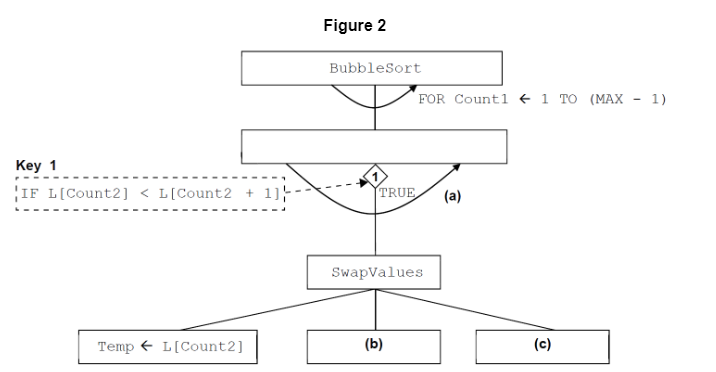
\includegraphics[width=0.5\paperwidth]{C:/Users/Admin/Desktop/Github/question_bank/LyX/static/img/9569-NYJC-2020-P1-Q1}
\par\end{center}
\begin{enumerate}
\item {}
\begin{enumerate}
\item Describe the goal of this problem. \hfill{}{[}1{]}
\item How should the curved arrow \textbf{(a)} in \textbf{Figure 2} be labelled?
\hfill{}{[}1{]}
\item What should be written in box \textbf{(b)} in \textbf{Figure 2}? \hfill{}{[}1{]}
\item What should be written in box\textbf{ (c)} in \textbf{Figure 2}? \hfill{}{[}1{]}
\end{enumerate}
\end{enumerate}
A new Bubble Sort routine is developed using the structure chart shown
in \textbf{Figure 2}.
\begin{enumerate}
\item[(b)] What value will be in \texttt{L{[}1{]} }when this Bubble Sort routine
has finished executing on the array \texttt{L} shown in \textbf{Figure
1}? \hfill{}{[}1{]}
\item[(c)]  A Bubble Sort routine, based on the structure chart in \textbf{Figure
2}, always completes \texttt{MAX - 1} passes through the array. Often,
this number of passes is not required, as the contents of the array
will be sorted after fewer passes have been made. If a pass is made
through the array during which no swaps need to be made, then the
array has been sorted.

Describe the changes that need to be made to the Bubble Sort routine
so that it will only complete the minimum number of passes through
the array that are needed to fully sort the contents of the array.
\hfill{} {[}3{]}
\item[(d)] The Bubble Sort routine can also be implemented using recursion. 
\begin{enumerate}
\item Define what is meant by a recursive function. \hfill{} {[}2{]}
\item Using pseudocode, write a recursive Bubble Sort routine.\hfill{}
{[}3{]}
\item Explain a disadvantage of a recursive Bubble Sort function over an
iterative one.\hfill{} {[}2{]}
\item Name and describe another recursive sort algorithm. \hfill{} {[}5{]}
\end{enumerate}
\end{enumerate}

 \newpage 

\item \textbf{{[}NYJC/PRELIM/9569/2020/P1/Q2{]} }

In Morse code, each letter of the alphabet is represented by a unique
combination of dots and dashes. Study the following table carefully:
\noindent \begin{center}
\begin{tabular}{|c|c|c|}
\hline 
\textbf{Letter} & \textbf{Morse Code} & \tabularnewline
\hline 
\hline 
A & \texttt{. -} & dot dash\tabularnewline
\hline 
B & \texttt{- . . .} & dash dot dot dot\tabularnewline
\hline 
C & \texttt{- . - .} & dash dot dash dot\tabularnewline
\hline 
D & \texttt{- . . .} & dash dot dot\tabularnewline
\hline 
\end{tabular}
\par\end{center}

A binary tree is used to represent this coding system. Each node,
except the root node, contains a letter of the alphabet. The position
of each letter in the tree is determined by its Morse code. Moving
from one node to another down the tree is done by traversing either
a left branch or a right branch. A left branch corresponds to a .
(dot) and a right branch corresponds to a -- (dash). 

The first three levels of the tree are shown below:
\begin{center}
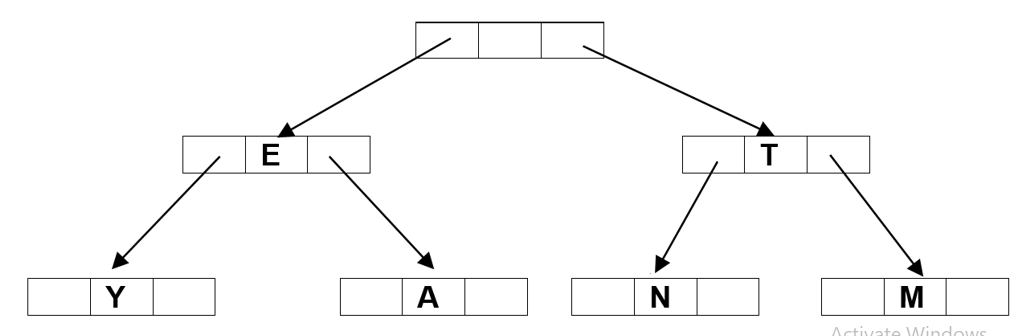
\includegraphics[width=0.5\paperwidth]{C:/Users/Admin/Desktop/Github/question_bank/LyX/static/img/9569-NYJC-2020-P1-Q2}
\par\end{center}
\begin{enumerate}
\item What are the Morse codes for the letters N and Y? \hfill{}{[}2{]}
\item Draw a diagram of the binary tree which clearly shows the position
of the letters D, C and B in the tree.\hfill{} {[}3{]}
\item {}
\begin{enumerate}
\item Explain why this binary tree representation is not the most suitable
data structure for performing English to Morse code conversion. \hfill{}{[}2{]}
\item Describe a better alternative and explain how the Morse code of a
letter could be found. \hfill{}{[}3{]}
\end{enumerate}
\end{enumerate}

 \newpage 

\item \textbf{{[}NYJC/PRELIM/9569/2020/P1/Q3{]} }

The algorithm represented using pseudo-code in \textbf{Figure 3} describes
a method to convert two hexadecimal numbers into decimal. The subroutine
\texttt{ToDecimal} used in\textbf{ Figure 3} is shown in \textbf{Figure
4} and the built-in subroutine \texttt{ASCII} is explained in \textbf{Table
1}. 
\noindent \begin{center}
\textbf{Figure 3} 
\par\end{center}

\noindent %
\noindent\begin{minipage}[t]{1\columnwidth}%
\texttt{FOR Count <- 1 TO 2 }

\texttt{\qquad{}INPUT HexString }

\texttt{\qquad{}Number <- 0 }

\texttt{\qquad{}FOR EACH HexDigit IN HexString }

\texttt{\qquad{}\qquad{}Value <- ToDecimal(HexDigit) }

\texttt{\qquad{}\qquad{}Number <- Number {*} 16 + Value }

\texttt{\qquad{}ENDFOR }

\texttt{\qquad{}OUTPUT Number }

\texttt{ENDFOR}%
\end{minipage}

The \texttt{FOR EACH} command steps through each character in a string
working from left to right. 
\noindent \begin{center}
\textbf{Figure 4} 
\par\end{center}

\noindent %
\noindent\begin{minipage}[t]{1\columnwidth}%
\texttt{SUBROUTINE ToDecimal(HexDigit)}

\texttt{\qquad{}IF HexDigit = \textquotedbl A\textquotedbl{} THEN }

\texttt{\qquad{}\qquad{}Value <- 10}

\texttt{\qquad{}ELSEIF HexDigit = \textquotedbl B\textquotedbl{}
THEN }

\texttt{\qquad{}\qquad{}Value <- 11}

\texttt{\qquad{}ELSEIF HexDigit = \textquotedbl C\textquotedbl{}
THEN}

\texttt{\qquad{}\qquad{}Value <- 12}

\texttt{\qquad{}ELSEIF HexDigit = \textquotedbl D\textquotedbl{}
THEN }

\texttt{\qquad{}\qquad{}Value <- 13}

\texttt{\qquad{}ELSEIF HexDigit {*} \textquotedbl E\textquotedbl{}
THEN }

\texttt{\qquad{}\qquad{}Value <- 14}

\texttt{\qquad{}ELSEIF HexDlgit = \textquotedbl F\textquotedbl{}
THEN }

\texttt{\qquad{}\qquad{}Value <- 15}

\texttt{\qquad{}ELSEIF HexDigit IN (\textquotedbl 0\textquotedbl ,
\textquotedbl l\textquotedbl , ..., \textquotedbl 9\textquotedbl{]}
THEN }

\texttt{\qquad{}\qquad{}Value <- ASCII(HexDigit) - 48}

\texttt{\qquad{}ELSE }

\texttt{\qquad{}\qquad{}Value <- -1}

\texttt{\qquad{}ENDIF}

\texttt{\qquad{}RETURN Value}

\texttt{ENDSUBROUTINE}%
\end{minipage}
\noindent \begin{center}
\textbf{Table 1} 
\par\end{center}

\noindent \begin{center}
\begin{tabular}{|c|c|}
\hline 
Subroutine used in Figure 4 & Description\tabularnewline
\hline 
\hline 
ASCII(Char) & Returns the ASCII code or the chal passed as a parameter. Example:
\texttt{ASCII (\textquotedbl l\textquotedbl )} returns \texttt{49}\tabularnewline
\hline 
\end{tabular}
\par\end{center}
\begin{enumerate}
\item Copy and complete the following table by hand-tracing the algorithm
in Figure 3. Use \textquotedbl\texttt{A2}\textquotedbl{} and \textquotedbl\texttt{1G}\textquotedbl{}
as input strings. You may not need to use all the rows. 
\noindent \begin{center}
\begin{tabular}{|c|c|c|c|c|c|}
\hline 
\texttt{\textbf{Count}} & \texttt{\textbf{HexString}} & \texttt{\textbf{Number}} & \texttt{\textbf{HexDigit}} & \texttt{\textbf{Value}} & \texttt{\textbf{Output}}\tabularnewline
\hline 
 &  &  &  &  & \tabularnewline
\hline 
 &  &  &  &  & \tabularnewline
\hline 
\multicolumn{6}{c}{$\vdots$}\tabularnewline
\end{tabular}
\par\end{center}

\hfill{}{[}6{]}
\item Explain how the algorithm in Figure 3 has attempted to deal with the
conversion of \textquotedbl\texttt{1G}\textquotedbl{} into decimal
and why this method is not fully effective. \hfill{} {[}2{]}
\item Other than a trace table, describe two other debugging methods a programmer
can use to find bugs in his code. \hfill{} {[}4{]}
\end{enumerate}

 \newpage 

\item \textbf{{[}NYJC/PRELIM/9569/2020/P1/Q4{]} }

Company X sells merchandise to wholesale and retail outlets. Wholesale
customers receive a two percent discount on all orders. The company
also encourages both wholesale and retail customers to pay cash on
delivery by offering a two percent discount for this method of payment.
Another two percent discount is given on orders of 50 or more units.
Discounts can be stacked for each order.
\begin{enumerate}
\item Create a decision table to show these conditions and actions. \hfill{}
{[}4{]}
\item Write pseudo-code to implement a function \texttt{ComputeDiscount}
that takes in the appropriate parameters and returns the message \textquotedblleft \texttt{Discount
rate is X\%}\textquotedblright{} where \texttt{X} is the calculated
discount. \hfill{}{[}6{]}
\item Draw a system flowchart of your pseudo-code in \textbf{(b)}. \hfill{}{[}4{]}
\end{enumerate}

 \newpage 

\item \textbf{{[}NYJC/PRELIM/9569/2020/P1/Q5{]} }

Athletes, who are members of teams, compete in running events, which
are held at fixtures throughout the year. For example, athlete 15
might compete in the Girls\textquoteright{} 1500m Under 18 race in
the fixture at National Stadium on 12 September 2020.

A relational database is used to store the details of which athletes
enter each event at each fixture. The relations used in the database
are shown in \textbf{Figure 5}.
\noindent \begin{center}
\textbf{Figure 5}
\par\end{center}

\texttt{Athlete(}\texttt{\uline{AthleteID}}\texttt{, Surname, Forename,
DateOfBirth, Gender, TeamName) }

\texttt{EventType(}\texttt{\uline{EventTypeID}}\texttt{, Gender,
Distance, AgeGroup) }

\texttt{Fixture(}\texttt{\uline{FixtureID}}\texttt{, FixtureDate,
LocationName) }

\texttt{EventAtFixture(}\texttt{\uline{FixtureID}}\texttt{, }\texttt{\uline{EventTypeID}}\texttt{) }

\texttt{EventEntry(}\texttt{\uline{FixtureID}}\texttt{, }\texttt{\uline{EventTypeID}}\texttt{,
}\texttt{\uline{AthleteID}}\texttt{) }
\begin{itemize}
\item Each \texttt{Athlete}, \texttt{EventType} and \texttt{Fixture} is
identified by a unique identity number, for example \texttt{AthleteID}
for athletes. 
\item An \texttt{EventType} is a type of event, such as Boys\textquoteright{}
100m Under 15 race. 
\item If an athlete wants to take part in an event at a particular fixture,
then an entry is created in the \texttt{EventEntry} relation to represent
this. 
\end{itemize}
\textbf{Figure 6} shows an incomplete entity-relationship diagram
for part of the database. 
\noindent \begin{center}
\textbf{Figure 6}
\par\end{center}

\begin{center}
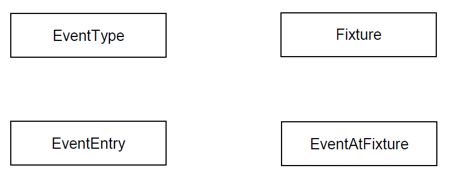
\includegraphics[width=0.5\paperwidth]{C:/Users/Admin/Desktop/Github/question_bank/LyX/static/img/9569-NYJC-2020-P1-Q5}
\par\end{center}
\begin{enumerate}
\item Copy and draw lines on \textbf{Figure 6} to show the degree of any
\textbf{three} relationships that exist between the four entities
shown. {[}3{]}
\item The following SQL statement is intended to make a table to represent
the Athlete relation. The statement contains some errors. 
\noindent \begin{center}
\textbf{Figure 7}
\par\end{center}

\noindent %
\noindent\begin{minipage}[t]{1\columnwidth}%
\texttt{CREATE TABLE Athlete ( }

\texttt{\qquad{}PRIMARY KEY AthleteID, }

\texttt{\qquad{}VARCHAR(50) Surname, }

\texttt{\qquad{}VARCHAR(30) Forename, }

\texttt{\qquad{}DATE DateOfBirth, }

\texttt{\qquad{}VARCHAR(6) Gender, }

\texttt{\qquad{}VARCHAR(30) TeamName }

\texttt{) }%
\end{minipage}

You may assume that all of the data types used in \textbf{Figure 7}
are valid and the field lengths are appropriate. State \textbf{two}
errors that have been made. \hfill{}{[}2{]}
\item State two reasons why database designs, such as this one, are usually
normalised. \hfill{}{[}2{]}
\item A list is to be produced of the names of all athletes who are competing
in the fixture that is taking place on 17/09/20. The list must include
the \texttt{Surname}, \texttt{Forename} and \texttt{DateOfBirth} of
these athletes and no other details. The list should be presented
in alphabetical order by Surname. With reference to the database design
shown in Figure 3, write an SQL query to produce the list. \hfill{}{[}5{]}
\item An IT consultant is suggesting changing to the use of a NoSQL database
instead.
\begin{enumerate}
\item Describe two advantages that a NoSQL database have over a SQL database.
\hfill{} {[}4{]}
\item Explain with reasons if you agree or disagree with making the change.
\hfill{}{[}2{]}
\end{enumerate}
\end{enumerate}

 \newpage 

\item \textbf{{[}NYJC/PRELIM/9569/2020/P1/Q6{]} }

Computers connected to the Internet use the TCP/IP suite of protocols
for data transmission.
\begin{enumerate}
\item What is a protocol? {[}1{]}
\item The TCP/IP stack is divided into four layers. One of these is the
application layer protocol. \textbf{Table 1} shows four different
scenarios that all use the TCP/IP protocol. Complete \textbf{Table
1} by writing the name of the particular \textbf{application layer
protocol} that would be used to transfer data during each operation.
You must give a different answer in each case.
\noindent \begin{center}
\textbf{Table 2}
\par\end{center}

\noindent \begin{center}
\begin{tabular}{|c|l|c|}
\hline 
 & \textbf{Operation} & \textbf{Application Layer Protocol }\tabularnewline
\hline 
\hline 
\textbf{(i)} & Managing a server remotely  & \tabularnewline
\hline 
\textbf{(ii)} & Retrieving e-mail from an e-mail server & \tabularnewline
\hline 
\textbf{(iii)} & Viewing a sports news web page using a web browser  & \tabularnewline
\hline 
\textbf{(iv)} & Accessing your online bank account using a web browser & \tabularnewline
\hline 
\end{tabular}
\par\end{center}

{[}4{]}
\item A student uses the following URL to download a copy of a previous
year\textquoteright s Computing exam paper.

$\mathtt{\underset{A}{\underbrace{https}}://\underset{B}{\underbrace{www.nanyang.moe.sg}}\underset{C}{\underbrace{/gce/computing/2019H2Computing2.pdf}}}$
\begin{enumerate}
\item Describe the \textbf{three} labelled parts (\texttt{A}, \texttt{B}
and \texttt{C}) of this URL.. \hfill{} {[}3{]}
\item State the top-level domain part in the URL. \hfill{} {[}1{]}
\end{enumerate}
\item To access the exam paper, the student\textquoteright s computer might
need to make use of a Domain Name System (DNS) query which is transmitted
to a DNS server.
\begin{enumerate}
\item What is the role of a DNS server? . \hfill{}{[}2{]}
\item In some circumstances the student\textquoteright s computer will not
need to contact a remote DNS server to access a resource. Describe
\texttt{two} situations when a DNS query will \texttt{not} be sent
to a remote DNS server. . \hfill{}{[}2{]}
\end{enumerate}
\item In the process of requesting a web page, a browser will generate an
HTTP GET request.
\begin{enumerate}
\item In which layer of the TCP/IP stack is the browser operating? . \hfill{}{[}1{]}
\item Explain why the student\textquoteright s computer might need to make
several HTTP GET requests to display one web page. . \hfill{}{[}2{]}
\item The HTTP GET requests are being sent to port 80 on the remote machine.
The browser has been allocated a \textbf{client port number}. What
is meant by a client port number?. \hfill{} {[}1{]}
\end{enumerate}
\end{enumerate}

 \newpage 

\item \textbf{{[}NYJC/PRELIM/9569/2020/P1/Q7{]} }

Below is a numbered list of the names of some of the legislation that
applies in situations where computers are used:

1. Copyright, Designs and Patents Act 

2. Computer Misuse Act 

3. Regulation of Investigatory Powers Act 

4. Health and Safety Regulations 5. Data Protection Act

For each of the situations given below, identify the relevant legislation
which is being followed. Write the number that corresponds to the
appropriate legislation in each situation.
\begin{enumerate}
\item {}
\begin{enumerate}
\item Marcus wanted an MP3 of a recent song so he went to an online music
store. After paying he was able to immediately download the purchased
song. \hfill{}{[}1{]}
\item A new workstation is installed in an office and an assessment is performed
regarding the lighting for the workstation and the positioning of
the desk, monitor and chair. \hfill{}{[}1{]}
\item Mr Smith hands over his 50-character encryption key in response to
a request from the authorities investigating a fraud case. \hfill{}{[}1{]}
\end{enumerate}
\item The operators of a number of multi-storey car parks have installed
systems to scan and recognise number plates. The system is used at
both the entrance and exit of the car parks so that the arrival and
leaving times can be recorded.

Customers can set up an account so that money is automatically debited
when their car number plate is recognised as the car leaves the car
park. Customers who do not have an account can use their mobile phones
to pay the car parking fees by sending a text message to a specified
number with their number plate details and length of stay.

As these car parks are based around Singapore, the company also collects
location specific data. 
\begin{enumerate}
\item The company will need to follow the Data Protection Act as they will
be storing personal data. What is meant by personal data? \hfill{}{[}1{]}
\item Why might the storing of number plate details, mobile phone numbers
and location specific data be a concern for privacy campaigners? \hfill{}
{[}2{]}
\end{enumerate}
\item Explain with specific examples why a code of conduct for computing
professionals is necessary. \hfill{} {[}3{]}
\end{enumerate}

 \newpage 

\item \textbf{{[}NYJC/PRELIM/9569/2020/P2/Q1{]} }

The task is to implement a hash table to retrieve data about waste
disposal in Singapore. 

For each of the sub-tasks, add a comment statement, at the beginning
of the code using the hash symbol '\texttt{\#}', to indicate the sub-task
the program code belongs to, for example:
\noindent \begin{center}
\begin{tabular}{c|l|}
\cline{2-2} 
\multirow{2}{*}{\texttt{In{[}1{]}:}} & \texttt{\# Task 1.1}\tabularnewline
 & \texttt{Program Code}\tabularnewline
\cline{2-2} 
\multirow{2}{*}{\texttt{In{[}2{]}:}} & \texttt{\# Task 1.2}\tabularnewline
 & \texttt{Program Code}\tabularnewline
\cline{2-2} 
\multirow{2}{*}{\texttt{In{[}3{]}:}} & \texttt{\# Task 1.3}\tabularnewline
 & \texttt{Program Code}\tabularnewline
\cline{2-2} 
\multicolumn{1}{c}{} & \multicolumn{1}{l}{\texttt{Output:}}\tabularnewline
\end{tabular}
\par\end{center}

The file \texttt{waste.csv} contains the following fields in each
line: 

\texttt{Year \textendash{} \textquotedblleft YYYY\textquotedblright{} }

\texttt{Waste Disposed Of \textendash{} \textquotedblleft Numeric\textquotedblright{}
(Million Tons) }

\texttt{Waste Recycled \textendash{} \textquotedblleft Numeric\textquotedblright{}
(Million Tons) }

The first line of the file contains the headings. 

\subsection*{Task 1.1 }

Write a program to: 
\begin{itemize}
\item read data from \texttt{waste.csv} 
\item into a hash table of size 20 
\item by creating a function \texttt{GetKeyAddress(Year)} to generate the
hash address 
\item and directly inserting the data into the correct location in the hash
table 
\item taking care of any potential collisions using any suitable methods 
\end{itemize}
Display the contents of the hash table showing the data from the first
slot to the last slot. \hfill{}{[}14{]}

\subsection*{Task 1.2}

Create a menu with the following options: 
\begin{enumerate}
\item[1.] \texttt{ Get Waste Disposed and Recycled by year }
\item[2.] \texttt{ Display year(s) where Recycled waste > Waste disposed }
\item[3.] \texttt{ Return Average waste disposed between two years }
\item[4.] \texttt{ -1 to Exit }
\end{enumerate}
\begin{itemize}
\item implement the functions for each menu choice. 
\item use only direct access to retrieve data for options 1 and 3. 
\item option 1 and 3 requires asking users to input in the year(s). 
\item validate the user input. 
\item test option 1 with the year 2007 and show the output. 
\item test option 3 with the range 2002 to 2008 and show the output. 
\item show the output for option 2. \hfill{}{[}10{]}
\end{itemize}
Save your program code and output for Task 1 as 

\texttt{TASK1\_<your name>.ipynb }

 \newpage 

\item \textbf{{[}NYJC/PRELIM/9569/2020/P2/Q2{]} }

A school library stores the following data in a file named \texttt{story.csv}: 

\begin{tabular}{ll}
\textbf{Field} & \textbf{Format}\tabularnewline
book\_title & text\tabularnewline
text subject & text\tabularnewline
author\_name & text\tabularnewline
published & \textquoteleft YYYY\textquoteright{} (year) \tabularnewline
\end{tabular}

Merge sort is an efficient sorting algorithm which falls under divide
and conquer paradigm and produces a stable sort. It operates by dividing
a large array into two smaller subarrays and then recursively sorting
the subarrays. 

For each of the sub-tasks, add a comment statement at the beginning
of the code using the hash symbol '\texttt{\#}', to indicate the sub-task
the program code belongs to, for example: 
\noindent \begin{center}
\begin{tabular}{c|l|}
\cline{2-2} 
\multirow{2}{*}{\texttt{In{[}1{]}:}} & \texttt{\# Task 2.1}\tabularnewline
 & \texttt{Program Code}\tabularnewline
\cline{2-2} 
\multirow{2}{*}{\texttt{In{[}2{]}:}} & \texttt{\# Task 2.2}\tabularnewline
 & \texttt{Program Code}\tabularnewline
\cline{2-2} 
\end{tabular}
\par\end{center}

\subsection*{Task 2.1 }

Write program code to: 
\begin{itemize}
\item read data from \texttt{story.csv} into an array of records. 
\item ask user to input in which field to sort the records by.
\item validate that the choice must be \texttt{\textquoteleft B\textquoteright },
\texttt{\textquoteleft S\textquoteright }, \texttt{\textquoteleft A\textquoteright },
or \texttt{\textquoteleft P\textquoteright{}} representing \texttt{book\_title},
\texttt{subject}, \texttt{author\_name} and \texttt{published} fields. 
\item implement a \texttt{MergeSort(ArrayData, Sortby)} function that takes
in two parameters, \texttt{ArrayData} (array of records) and \texttt{Sortby},
and sorts the records in ascending order according to the specified
field. \texttt{MergeSort(ArrayData, Sortby)} will return the sorted
\texttt{ArrayData} using a mergesort algorithm to do the sorting. 
\item display \texttt{ArrayData}. 
\item test your program twice and show your output for sorting by \texttt{subject}
and by \texttt{author\_name}. \hfill{} {[}12{]}
\end{itemize}

\subsubsection*{Task 2.2 }

Write program code to: 
\begin{itemize}
\item implement a \texttt{QuickSort(ArrayData)} function that uses the quicksort
algorithm to sort the \texttt{ArrayData} by \texttt{book\_title} in
descending order. \hfill{} {[}8{]}
\end{itemize}
Design 2 test cases to test your QuickSort(ArrayData) function and
explain the purpose of the test data. Show the output of your test
cases. \hfill{}{[}4{]}

Save your program code and output for Task 2 as 

\texttt{TASK2\_<your name>.ipynb}

 \newpage 

\item \textbf{{[}NYJC/PRELIM/9569/2020/P2/Q3{]} }

You are to create a song playlist using a doubly linked list implemented
using Object-Oriented Programming (OOP). The doubly linked list data
structure is a linked list made up of nodes with two pointers pointing
to the next and previous element. 
\begin{center}
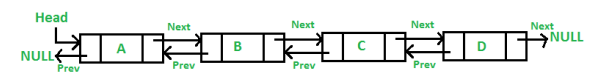
\includegraphics[width=0.5\paperwidth]{C:/Users/Admin/Desktop/Github/question_bank/LyX/static/img/9569-NYJC-2020-P2-Q3-1}
\par\end{center}

A doubly linked list allows traversal of nodes in both direction which
is not possible in a singly linked list. For example, a user can go
forward or backwards to play the next or previous song.

The \texttt{node}, will store the following data: 
\begin{itemize}
\item \texttt{title (str) }
\item \texttt{prev (node) }
\item \texttt{next (node)} 
\end{itemize}
The class, \texttt{SongPlaylist}, will store the following data: 
\begin{itemize}
\item a doubly linked list of \texttt{node} objects. 
\item \texttt{head} pointer, pointing to the first \texttt{node} in the
doubly linked list. 
\end{itemize}
The class \texttt{SongPlaylist} has the following methods: 
\begin{itemize}
\item \texttt{insert(SongPlaylist, title: str)} adds a song title at the
beginning of the list. 
\item \texttt{insertafter(SongPlaylist, searchtitle: str, newtitle: str)}
adds a song title after \texttt{searchtitle}.
\item \texttt{display(SongPlaylist)} outputs out the playlist. 
\end{itemize}
For each of the sub-tasks, add a comment statement, at the beginning
of the code using the hash symbol '\#', to indicate the sub-task the
program code belongs to, for example: 
\noindent \begin{center}
\begin{tabular}{c|l|}
\cline{2-2} 
\multirow{2}{*}{\texttt{In{[}1{]}:}} & \texttt{\# Task 3.1}\tabularnewline
 & \texttt{Program Code}\tabularnewline
\cline{2-2} 
\multirow{2}{*}{\texttt{In{[}2{]}:}} & \texttt{\# Task 3.2}\tabularnewline
 & \texttt{Program Code}\tabularnewline
\cline{2-2} 
\multirow{2}{*}{\texttt{In{[}3{]}:}} & \texttt{\# Task 3.3}\tabularnewline
 & \texttt{Program Code}\tabularnewline
\cline{2-2} 
\multicolumn{1}{c}{} & \multicolumn{1}{l}{\texttt{Output:}}\tabularnewline
\end{tabular}
\par\end{center}

\subsection*{Task 3.1 }

Write program code to define classes to implement the song playlist.
The figures below show the links that must be updated for the insert
and insertafter methods: 

Inserting at the beginning of the list
\begin{center}
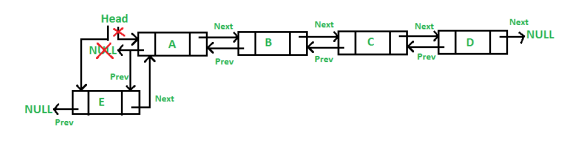
\includegraphics[width=0.5\paperwidth]{C:/Users/Admin/Desktop/Github/question_bank/LyX/static/img/9569-NYJC-2020-P2-Q3-2}
\par\end{center}

Inserting after a given node
\begin{center}
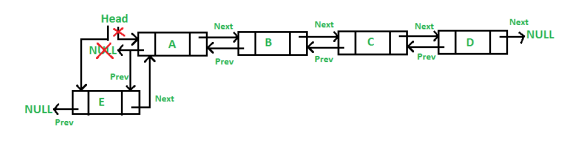
\includegraphics[width=0.5\paperwidth]{C:/Users/Admin/Desktop/Github/question_bank/LyX/static/img/9569-NYJC-2020-P2-Q3-3}
\par\end{center}

\noindent \begin{center}
\textcolor{white}{.}\hfill{}{[}10{]} 
\par\end{center}

The program has the following menu: 
\begin{enumerate}
\item[1.] \texttt{ Create New Song Playlist }
\item[2.] \texttt{ Add a song in front }
\item[3.] \texttt{ Add a song after }
\item[4.] \texttt{ Display Playlist }
\item[5.] \texttt{ -1 to End }
\end{enumerate}
Option 1 will prompt the user to enter the name of the new playlist. 

Option 2 will prompt the user to enter the song title and the name
of the playlist. 

Option 3 will prompt the user to enter the name of the playlist, existing
song title, and the new song title to be inserted after the existing
song title. 

Option 4 will prompt the user to enter the name of the playlist to
be displayed and output accordingly. 

\subsection*{Task 3.2 }

Write program code to: 
\begin{itemize}
\item display the main menu. 
\item input the choice by the user. 
\item run the appropriate code to carry out the task for the choice made.
\hfill{}{[}4{]}
\end{itemize}
Test your program by creating a new playlist called \texttt{MJ} and
add in the following titles in order: \texttt{\textquotedblleft Heal
the World\textquotedblright }, \texttt{\textquotedblleft Thriller\textquotedblright },
\texttt{\textquotedblleft Beat It\textquotedblright }. Show your output
by displaying the playlist.\hfill{}{[}2{]}

\subsection*{Task 3.3 }

Extend your program by writing a function \texttt{insertionSort(Playlist)}
that will sort the song titles in ascending order. 

The algorithm for this \texttt{insertionSort} is given below: 
\begin{enumerate}
\item[1)]  Create an empty \texttt{sorted} doubly linked list. 
\item[2)]  Traverse the given doubly linked list, do following for every node.
- Insert current node in sorted way in \texttt{sorted} doubly linked
list. 
\item[3)]  Change head of given linked list to head of \texttt{sorted} list. 
\end{enumerate}
Write program code to implement \texttt{insertionSort(Playlist)}.
\hfill{}{[}6{]}

Save your program code and output for Task 3 as 

\texttt{TASK3\_<your name>.ipynb}

 \newpage 

\item \textbf{{[}NYJC/PRELIM/9569/2020/P2/Q4{]} }

A school wants to create a database to allow students to register
for different enrichment activities that will be held on the school\textquoteright s
Enrichment Day. An enrichment activity falls under one of three categories
-- Arts, Cultural, and Sports. 

It is expected that the database should be normalised. 

When a student registers for an activity, the following information
is recorded: 
\begin{itemize}
\item \texttt{StudentID} - unique 6-digit register number of the student. 
\item \texttt{Type} - type of activity (\texttt{'A\textquoteright }, \texttt{\textquoteleft C\textquoteright{}}
or \texttt{'S'}). 
\item \texttt{Venue} - where the activity will be held. 
\item \texttt{Session} - whether the activity is conducted in the morning
or afternoon (\texttt{'AM'} means the morning session, and \texttt{'PM'}
means the afternoon session). 
\end{itemize}
For the Arts category, the following extra information is recorded: 
\begin{itemize}
\item \texttt{Performance} -- \textquotedblleft \texttt{True}\textquotedblright{}
for performance arts, \textquotedblleft \texttt{False}\textquotedblright{}
for visual arts. 
\end{itemize}
For Cultural, the following extra information is recorded:
\begin{itemize}
\item \texttt{Race} -- which race the culture belongs to. 
\end{itemize}
For Sports, the following extra information is recorded: 
\begin{itemize}
\item \texttt{Contact} -- \textquotedblleft C\textquotedblright{} to denote
contact sports, \textquotedblleft NC\textquotedblright{} to denote
non-contact sports. 
\item \texttt{Cost} - the amount of money in dollars (not more than \$50)
the student must pay the instructor. 
\end{itemize}
The information is to be stored in four different tables: 

\texttt{Registration }

\texttt{Arts}

\texttt{Cultural }

\texttt{Sports }

\subsection*{Task 4.1}

Create an SQL file called\texttt{ TASK4\_l\_<your name>.sql} to show
the SQL code to create the database\texttt{ register.db} with the
four tables. The table, \texttt{Registration}, must use \texttt{StudentID}
as its \textbf{primary key}. The other tables must refer to the \texttt{StudentID}
as a \textbf{foreign key}.

Save your SQL code as 

\texttt{TASK4\_1\_<your name>.sql}\hfill{} {[}5{]}

\subsection*{Task 4.2 }

The school wants to allow students to register over the internet.
The form design for the webpage is shown below: 
\begin{center}
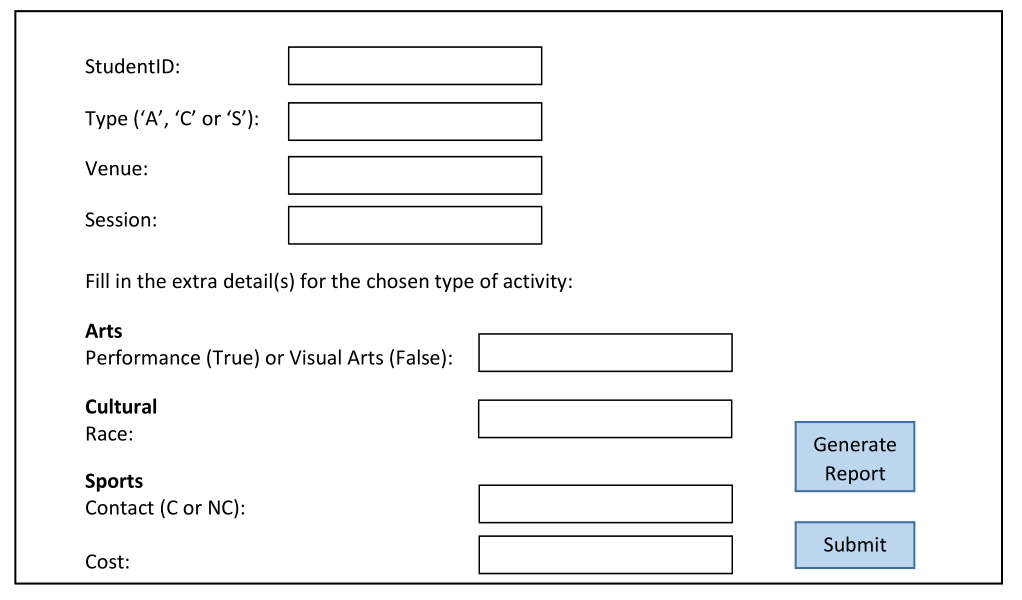
\includegraphics[width=0.5\paperwidth]{C:/Users/Admin/Desktop/Github/question_bank/LyX/static/img/9569-NYJC-2020-P2-Q4}
\par\end{center}

Write a Python program and the necessary files to create a web application
that: 
\begin{itemize}
\item accepts the input from the web form (assume input is keyed in correctly) 
\item updates the registration details into \texttt{register.db} 
\item creates and returns a HTML document that enables the web browser to
display a table tabulating the \texttt{StudentID} and \texttt{Type}
of activity registered for the morning session. 
\end{itemize}
Save your Python program as

\texttt{TASK4\_2\_<your name>.py} with any additional files / sub-folders
as needed in a folder named \texttt{TASK4\_2\_<your name>} \hfill{}{[}12{]}

\subsection*{Task 4.3 }

Test your web application by entering the following records via the
form\textquoteright s submit button: 

\texttt{192701, A, Hall, AM, True }

\texttt{192703, A, MPR, PM, False }

\texttt{192723, S, Field, AM, C, 20 }

\texttt{192803, C, 5-56, AM, Malay }

\texttt{192820, S, 5-60, PM, NC, 15 }

\texttt{193005, C, LT4, PM, Chinese }

\texttt{193006, C, LT4, PM, Chinese} 

Save the output of the program when the user clicks on the \textquotedblleft Generate
Report\textquotedblright{} button as \texttt{TASK4\_3\_<your name>.html}\hfill{}
{[}3{]}

\subsection*{Task 4.4 }

Write SQL code to count the number of different races for the cultural
activities. Run this query. 

Save this code as 

\texttt{TASK4\_4\_<your name>.sql} \hfill{}{[}4{]}

 \newpage 

\item \textbf{{[}YIJC/PRELIM/9569/2020/P1/Q1{]} }

A list of data items is stored in a hash table using an array \texttt{Values}.
The following pseudocode describes an algorithm for searching the
table using the hashing function \texttt{Hash}. 

\noindent\begin{minipage}[t]{1\columnwidth}%
\texttt{01 Index <- Hash(Key) }

\texttt{02 WHILE Values{[}Index{]} <> Key }

\texttt{03 \qquad{}Index <- Index + 1}

\texttt{04 ENDWHILE }

\texttt{05 Return Values{[}Index{]} }%
\end{minipage}
\begin{enumerate}
\item Explain the situations when \textquotedbl\texttt{Values{[}Index{]}
<> Key\textquotedbl} in line \texttt{02} will be \texttt{True}.
\hfill{}{[}2{]}
\item describe the two problems with this algorithm. \hfill{}{[}2{]}
\item Without writing any program code, describe the modifications required
to overcome each of the problems stated in (b). \hfill{}{[}4{]}
\end{enumerate}

 \newpage 

\item \textbf{{[}YIJC/PRELIM/9569/2020/P1/Q2{]} }

An array \texttt{seq} contains a list of sorted data items except
the last element. \texttt{{[}1,2,5,8,9,6{]}} is an example of such
an array. 

The function \texttt{sortInner} takes two parameters, the array \texttt{seq}
and the index position \texttt{j} of the last element, and returns
the mutated array \texttt{seq}. 

\noindent\begin{minipage}[t]{1\columnwidth}%
\texttt{def sortInner(seq, j): }

\texttt{\qquad{}if j == 0: }

\texttt{\qquad{}\qquad{}return seq }

\texttt{\qquad{}else: }

\texttt{\qquad{}\qquad{}if seq{[}j{]} <= seq{[}j-1{]}: }

\texttt{\qquad{}\qquad{}\qquad{}seq{[}j{]}, seq{[}j-1{]} = seq{[}j-1{]},
seq{[}j{]} }

\texttt{\qquad{}return sortInner(seq, j-1)}%
\end{minipage} 
\begin{enumerate}
\item State what is meant by a recursive function.\hfill{} {[}2{]} 
\item Describe what happens when the function \texttt{sortInner({[}1,2,5,8,9,6{]},5)}
is executed. \hfill{}{[}2{]} 
\item Write a recursive function \texttt{insertionSort} for the Insertion
Sort algorithm by using the given function \texttt{sortInner(seq,j}).\hfill{}
{[}2{]} 
\item Explain whether the Insertion Sort algorithm in \textbf{(c)} is performing
an \textquotedbl in-place\textquotedbl{} or \textquotedbl non in-place\textquotedbl{}
sorting and whether it is stable or unstable.\hfill{} {[}4{]} 
\item State and explain the efficiencies of the Insertion Sort algorithm
in \textbf{(c)} in the worst case scenario, using the Big-O notation
for the time complexity. \hfill{}{[}2{]} 
\end{enumerate}

 \newpage 

\item \textbf{{[}YIJC/PRELIM/9569/2020/P1/Q3{]} }

A wildlife information application is being developed to store and
display information about birds. The application uses a binary search
tree to store the name of the bird. 
\begin{enumerate}
\item The binary search tree has its data inserted in the following order. 

\texttt{Magpie }

\texttt{Cockatiel }

\texttt{Jay }

\texttt{Pigeon }

\texttt{Mynah }

\texttt{Crow }

\texttt{Albatross }

\texttt{Quail }

Draw the binary search tree. \hfill{}{[}4{]}
\item The binary search tree in part \textbf{(a)} can be implemented using
object-oriented programming that involves the use of two pointers
and an array. 
\begin{enumerate}
\item Describe the purpose of the two pointers in the implementation of
the binary search tree class. \hfill{} {[}2{]}
\item Describe the purpose of the array in the implementation of the binary
search tree class. \hfill{}{[}1{]}
\end{enumerate}
\item {}
\begin{enumerate}
\item List the nodes, in order, that are visited for an in-order traversal.
\hfill{}{[}2{]}
\item State the property exhibited by the list of items produced in part
(c)(i). \hfill{}{[}1{]}
\end{enumerate}
\item Describe an algorithm, using pseudocode, which uses a stack to perform
an in- order traversal for the tree \hfill{} {[}5{]}
\end{enumerate}

 \newpage 

\item \textbf{{[}YIJC/PRELIM/9569/2020/P1/Q4{]} }

\emph{HoLi Tea} is a popular chain selling a wide variety of bubble
tea. Each drink is categorised by the flavor (e.g. brown sugar, peppermint,
lemon \dots ), the type of tea leaves used (e.g. green tea, red tea,
black tea \dots ), the pearl options (e.g. black pearl, white pearl,
or no pearl) and the price. 

There are two variants of bubble tea: Milk Tea and Fruit Tea. Each
milk tea has a specific type of milk used (e.g. fresh milk, condensed
milk) and some milk tea come with pudding. Some fruit tea include
cultured milk. 

The owner of HoLi Tea intends to use object-oriented programming language
to store and process the information on the types of drink in the
self-ordering web application system. 

The base class \texttt{BUBBLE\_TEA} has a method to display the properties
of the bubble tea. 
\begin{enumerate}
\item {}
\begin{enumerate}
\item Draw a UML class diagram showing:\hfill{}{[}6{]}
\begin{itemize}
\item any derived classes and inheritance from the base class 
\item the properties needed in the base, and any derived classes 
\item suitable methods to support the system with at least one getter and
one setter method
\end{itemize}
\item Explain why inheritance is an important feature of object-oriented
programming.\hfill{} {[}2{]}
\item Explain why polymorphism is useful in object-oriented programming.
\hfill{}{[}2{]}
\end{enumerate}
\emph{HoLi Tea} has a loyalty programme to reward their regular customers.
Members are entitled to a 20\% discount for their purchases and a
free drink on their birthday. To pay tribute to the frontline workers
during the COVID-19 pandemic, all frontline workers are entitled to
a 20\% discount for their purchases, and those who are also members
will receive a free drink on any day. 
\item {}
\begin{enumerate}
\item Create a decision table showing all the possible conditions and actions.
\hfill{}{[}5{]}
\item Simplify your decision table by removing redundancies. \hfill{}{[}3{]}
\end{enumerate}
\end{enumerate}

 \newpage 

\item \textbf{{[}YIJC/PRELIM/9569/2020/P1/Q5{]} }

YI restaurant serves a variety of local dishes at reasonable prices
and plans to provide food delivery services to its customers via a
web application. A customer places an online order and an employee
will be assigned by the system to deliver the order to the customer.
The customer can choose to pay online when ordering or make cash payment
upon delivery. Customers can choose more than one dish in the same
online order and each order has a unique ID. 

At the time of ordering, the application records the following data: 
\begin{itemize}
\item Customer name, delivery address and email, if the customer has not
placed an online order before 
\item Customer ID 
\item Order date 
\item Order time 
\item Payment mode 
\item Dish and quantity 
\end{itemize}
The following shows an example of the order receipt which will be
sent to the customer\textquoteright s email address. 
\begin{center}
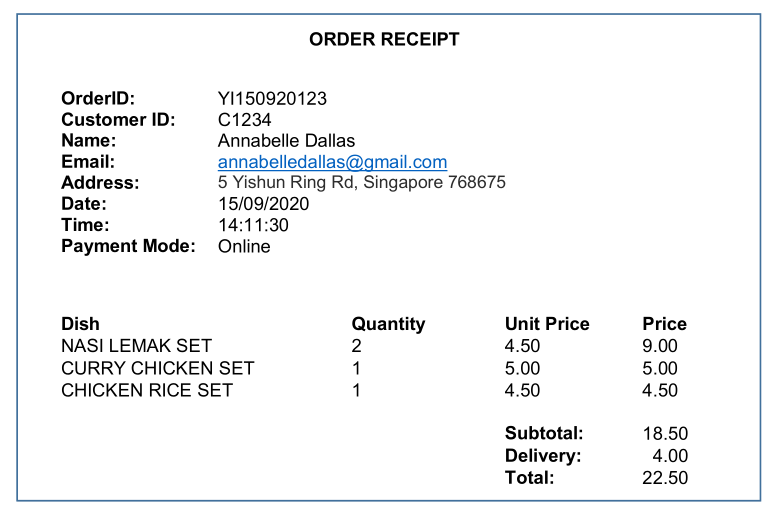
\includegraphics[width=0.5\paperwidth]{C:/Users/Admin/Desktop/Github/question_bank/LyX/static/img/9569-YIJC-2020-P1-Q5}
\par\end{center}

The restaurant assigns a unique ID to each employee and maintains
its employees\textquoteright{} information, such as their name, contact
number and bank account number. The restaurant keeps a record of the
employees\textquoteright{} delivery assignments, the date and time
when the order is successfully delivered to the customer. 
\begin{enumerate}
\item The company wants to model this application using a relational database. 
\begin{enumerate}
\item The database needs three tables to store the data for the customers\textquoteright{}
food order: \texttt{CUSTOMER}, \texttt{ORDER} and \texttt{FOOD}. 

Draw an Entity-Relationship (E-R) diagram showing the three tables
and the relationships between them. \hfill{}{[}2{]}
\item The database needs three tables to store the data for the employees\textquoteright{}
delivery assignment: \texttt{EMPLOYEE}, \texttt{ORDER} and \texttt{ASSIGNMENT}. 

Draw an Entity-Relationship (E-R) diagram showing the three tables
and the relationships between them. \hfill{}{[}2{]}
\item Draw the overall Entity-Relationship (E-R) diagram showing the five
tables and the relationships between them. \hfill{}{[}1{]}
\end{enumerate}
\item A table description can be expressed as: 

\texttt{TableName (}\texttt{\uline{Attribute1}}\texttt{, Attribute2{*},
Attribute3,...)} 

The primary key is indicated by underlining one or more attributes. 

Foreign keys are indicated using an asterisk or dashed underline. 

Write table descriptions for the five tables.\hfill{} {[}6{]}
\item Describe a method to protect data from loss or corruption.\hfill{}
{[}2{]}
\item Explain how Singapore\textquoteright s Personal Data Protection Act
(PDPA) protects the personal data of the customers and employees stored
in the database. \hfill{}{[}2{]}
\item Describe the impact of such food delivery applications on the society
and economy.\hfill{} {[}4{]}
\item With an increase in demand for food delivery, the restaurant wishes
to enhance the food delivery services to cater to the larger volume
of orders and to include more features in the application such as
real time location tracking of the food order and customers\textquoteright{}
review of the dishes, yet ensuring that the application maintains
fast performance. The restaurant is now considering using a NoSQL
DBMS instead of a relational database. 

State and explain \textbf{two} reasons why NoSQL DBMS may be more
suitable for the proposed scenario.\hfill{} {[}4{]}
\end{enumerate}

 \newpage 

\item \textbf{{[}YIJC/PRELIM/9569/2020/P1/Q6{]} }

A Web Developer is designing an online Sales portal for a company.
The customer needs to submit an online form to register before ordering
through the portal. 
\begin{center}
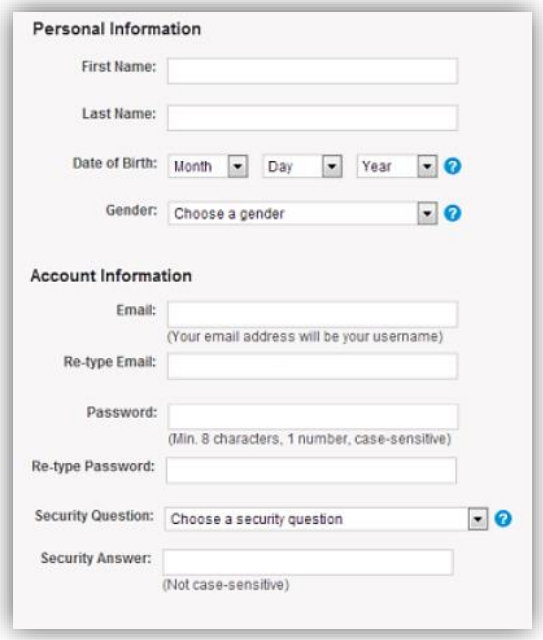
\includegraphics[width=0.25\paperwidth]{C:/Users/Admin/Desktop/Github/question_bank/LyX/static/img/9569-YIJC-2020-P1-Q6}
\par\end{center}
\begin{enumerate}
\item Explain the difference between data validation and data verification.
\hfill{}{[}2{]}
\item Describe two validation checks that the above form should perform
for the customer's inputs.\hfill{} {[}2{]}
\item Describe, with a specific example, how the customer's inputs are being
verified. \hfill{}{[}2{]}
\end{enumerate}
The web developer intends to use CAPTCHA for the above form 
\begin{center}
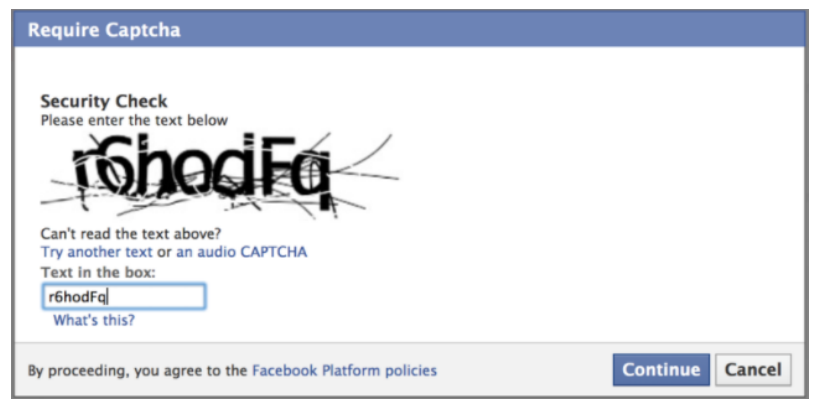
\includegraphics[width=0.3\paperwidth]{C:/Users/Admin/Desktop/Github/question_bank/LyX/static/img/9569-YIJC-2020-P1-Q6-2}
\par\end{center}
\begin{enumerate}
\item Explain what this added feature helps to verify. \hfill{}{[}2{]}
\item Describe the required server scripting to process the customer's input
on his email address and password. \hfill{}{[}4{]}
\item Describe the differences between a web application and a native application.
Explain how the developer should decide between designing a web or
a native application.\hfill{} {[}4{]}
\end{enumerate}

 \newpage 

\item \textbf{{[}YIJC/PRELIM/9569/2020/P1/Q7{]} }

The College\textquoteright s local area network (LAN) is connected
to the MOE Headquarter\textquoteright s LAN over the internet. 
\begin{center}
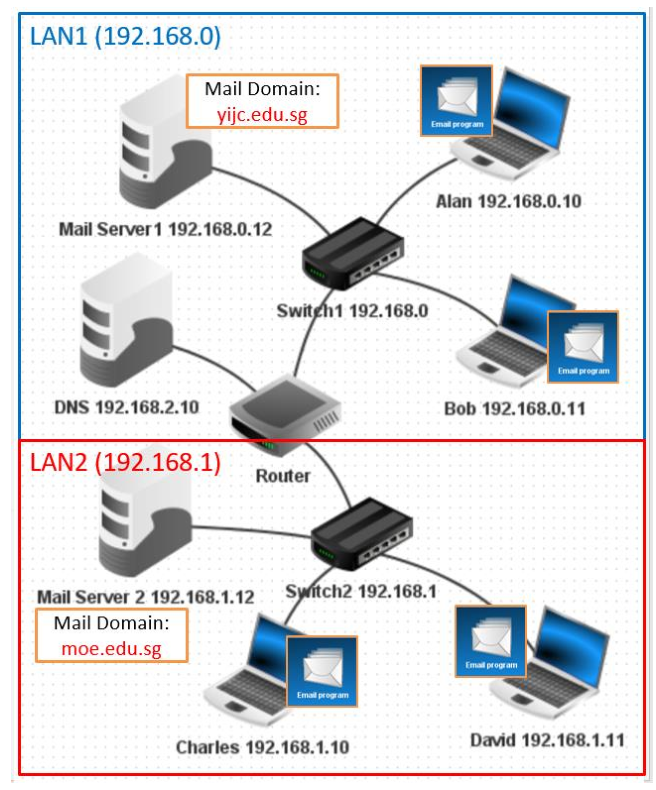
\includegraphics[width=0.5\paperwidth]{C:/Users/Admin/Desktop/Github/question_bank/LyX/static/img/9569-YIJC-2020-P1-Q7}
\par\end{center}

A staff in the college, Alan, sends an email to Charles who works
in the MOE Headquarter.
\begin{enumerate}
\item The following questions should take reference from the above network
diagram. 
\begin{enumerate}
\item Describe the function of the Domain Name System (DNS) server.\hfill{}
{[}1{]}
\item Explain how the router identifies that the MOE's Mail server is residing
in another network.\hfill{} {[}1{]}
\item Describe in detail how Alan's email is delivered and kept in the MOE's
Mail server.\hfill{} {[}2{]}
\item Describe how Charles eventually receive Alan\textquoteright s email.\hfill{}
{[}2{]}
\end{enumerate}
\item Charles forwards Alan\textquoteright s email to his colleague, David.
Describe how David could receive the email even when he is away from
the office. \hfill{}{[}2{]}
\end{enumerate}

 \newpage 

\item \textbf{{[}YIJC/PRELIM/9569/2020/P2/Q1{]} }

In a Battleship game, a player fires missiles within a region measuring
6 metres by 6 metres, represented with full-stops (\textquotedbl .\textquotedbl ),
to sink the ships. Each ship is represented by \textquotedbl\texttt{XXX}\textquotedbl .
The region is represented on the screen by a rectangular grid. Each
square metre of the region is represented by an x-coordinate and a
y-coordinate. The top left square metre of the region display has
\texttt{x = 0} and \texttt{y = 0}. 

\subsubsection*{Task 1.1}

In one of the games, three ships were positioned in the region as
given in the text file \texttt{GAME.TXT}. Write a program to read
in the data from this file, store it in a suitable data structure
and display on the screen as shown.

\noindent %
\noindent\begin{minipage}[t]{1\columnwidth}%
\texttt{. . . . . . }

\texttt{. . . . X . }

\texttt{X X X . X . }

\texttt{. . . . X . }

\texttt{. X X X . . }

\texttt{. . . . . . }%
\end{minipage}

\hfill{}{[}6{]}

\subsubsection*{Task 1.2}

During the game, the player cannot see the ships in the region.

\noindent %
\noindent\begin{minipage}[t]{1\columnwidth}%
\texttt{. . . . . . }

\texttt{. . . . . . }

\texttt{. . . . . . }

\texttt{. . . . . . }

\texttt{. . . . . . }

\texttt{. . . . . .}%
\end{minipage}

Write program code to allow the player to fire 5 missiles targeting
at specific locations, one at a time after observing each outcome.
The player will input an x-coordinate and y-coordinate for each targeted
location.

If the missile strikes any part of a ship, the damaged square metre
will be represented with an \textquotedbl\texttt{S}\textquotedbl ,
otherwise an \textquotedbl\texttt{O}\textquotedbl{} to represent
it has missed. A sunken ship will be represented by \textquotedbl\texttt{SSS}\textquotedbl .

\noindent %
\noindent\begin{minipage}[t]{1\columnwidth}%
one missile which missed the ship

\bigskip{}

\texttt{O . . . . .}

\texttt{. . . . . .}

\texttt{. . . . . .}

\texttt{. . . . . .}

\texttt{. . . . . .}

\texttt{. . . . . .}%
\end{minipage}

\noindent %
\noindent\begin{minipage}[t]{1\columnwidth}%
another missile which struck the ship

\bigskip{}

\texttt{O . . . . .}

\texttt{. . . . . .}

\texttt{. S . . . .}

\texttt{. . . . . .}

\texttt{. . . . . .}

\texttt{. . . . . .}%
\end{minipage}

The program code should also display the positions of all the ships
at the end of the game.

\noindent %
\noindent\begin{minipage}[t]{1\columnwidth}%
\texttt{O . . . . . }

\texttt{. . . . X . }

\texttt{S S S . X . }

\texttt{. . . . X . }

\texttt{. X X S . . }

\texttt{. . . . . .}%
\end{minipage}

\hfill{}{[}7{]} 

Download your program code and output for Task 1.1 and 1.2 as 

\texttt{Task1\_<your name>\_<centre number>\_<index number>.ipynb}

\subsubsection*{Task 1.3}

Write server and client program for this asymmetric Battleship game
where a server display the region and the player (the client) selects
the target locations for his missiles. After firing each missile,
the server returns an updated display for the region indicating a
strike or a miss. Once the player fires his last missile, the server
will display the positions of all the ships, together with the damages
and misses, and both the client and server quit the game. \hfill{}{[}12{]}

Download your server and client program code for Task 1.3 as

\texttt{Task1\_server\_<your name>\_<centre number>\_<index number>.py }

\texttt{Task1\_client\_<your name>\_<centre number>\_<index number>.py}

 \newpage 

\item \textbf{{[}YIJC/PRELIM/9569/2020/P2/Q2{]} }

The file \texttt{SONG.TXT} contains the lyrics of the song, Count
on me Singapore. The task is to read every word from the file, store
it in a suitable data structure, sort the words and perform searches
based on word and count.

\subsection*{Task 2.1}

Write program code to:
\begin{itemize}
\item read the words from the file and store them in a suitable data structure,
\item sort the words in alphabetical order using \textbf{quick sort}, 
\item write each word and their number of occurrence in a text file, WORDCOUNT.TXT,
where the next word is on a new line. {[}12{]}
\end{itemize}
A sample of the \texttt{WORDCOUNT.TXT} for the first 5 lines is as
follows:

\noindent %
\noindent\fbox{\begin{minipage}[t]{1\columnwidth - 2\fboxsep - 2\fboxrule}%
\texttt{a 5 }

\texttt{achieve 12 }

\texttt{air 1 }

\texttt{all 1 }

\texttt{and 9}%
\end{minipage}}

\subsection*{Task 2.2}

Write program code to:
\begin{itemize}
\item read the words and counts from the \texttt{WORDCOUNT.TX}T file 
\item allow the user to select the following options:

\noindent %
\noindent\begin{minipage}[t]{1\columnwidth}%
\texttt{1. Search for a word }

\texttt{2. Search for word(s) based on count}

\texttt{3. Quit program}%
\end{minipage}
\item take in user input for the word or the count 
\item if found, display the word and its count, else 
\item display \textquotedbl\texttt{Not Found}\textquotedbl{} display appropriate
error messages for invalid user input \hfill{}{[}6{]}
\end{itemize}

\subsection*{Task 2.3}

Design test data for your program written in \textbf{Task 2.2}, provide
evidence of testing that includes:
\begin{itemize}
\item search for a word that is contained in the file 
\item search for a word that is not contained in the file
\item search for word(s) with a count that is contained in the file 
\item search for word(s) with a count that is not contained in the file
\hfill{} {[}2{]}
\end{itemize}
Download your program code and output for Task 2 as 

\texttt{Task2\_<your name>\_<centre number>\_<index number>.ipynb}

 \newpage 

\item \textbf{{[}YIJC/PRELIM/9569/2020/P2/Q3{]} }

The task is to store words in nodes that is contained within a linked
list data structure. A node contains a word, the word category and
a next pointer. The pointers link the word items in proper grammatical
order based on their word category (\textquoteleft N\textquoteright :
noun, \textquoteleft V\textquoteright : verb, \textquoteleft D\textquoteright :
determiner, \textquoteleft J\textquoteright : adjective). The unused
nodes are linked as shown below. The first unused node is the position
where the new word item is to be stored.
\begin{center}
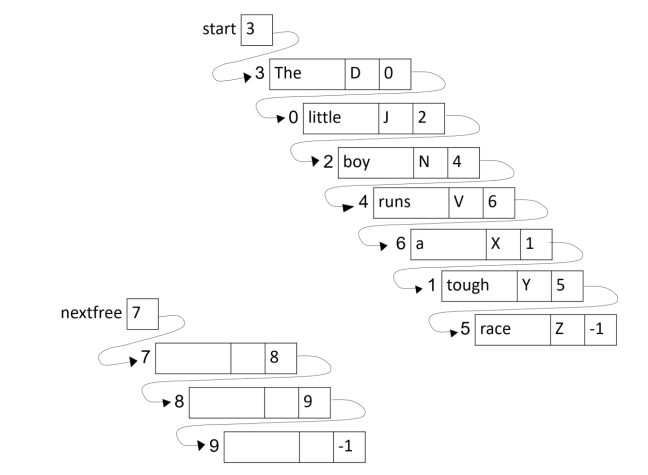
\includegraphics[width=0.5\paperwidth]{C:/Users/Admin/Desktop/Github/question_bank/LyX/static/img/9569-YIJC-2020-P2-Q3-1}
\par\end{center}

The diagram shows the linked list with:
\begin{itemize}
\item the words and their respective category inserted in the following
order: 
\begin{itemize}
\item \texttt{'little', 'J' }
\item \texttt{'tough', 'J' }
\item \texttt{'boy', 'N' }
\item \texttt{'The', 'D' }
\item \texttt{'runs', 'V' }
\item \texttt{'race', 'N' }
\item \texttt{'a', 'D'}
\end{itemize}
\item the unused nodes linked together
\end{itemize}
Each node is implemented as an instance of the class Node. The class
Node has the following UML class diagram:
\begin{center}
\begin{tabular}{|l|}
\hline 
\hspace{0.25\columnwidth}Node\tabularnewline
\hline 
\texttt{word: STRING}\tabularnewline
\texttt{category: STRING}\tabularnewline
\texttt{next: INTEGER}\tabularnewline
\hline 
\texttt{constructor()}\tabularnewline
\texttt{set\_word(w: STRING)}\tabularnewline
\texttt{set\_category(c: STRING)}\tabularnewline
\texttt{set\_next(n: INTEGER)}\tabularnewline
\texttt{get\_word(): STRING}\tabularnewline
\texttt{get\_category(): STRING}\tabularnewline
\texttt{get\_next(): INTEGER}\tabularnewline
\hline 
\end{tabular}
\par\end{center}

The \texttt{LinkedList} class is implemented as follows: 
\begin{itemize}
\item Attributes
\begin{itemize}
\item \texttt{sentence : ARRAY{[}0:9{]} of Node -} The linked list data
structure that contains 10 nodes.
\item \texttt{start : INTEGER} - Index for the start position of the linked
list. 
\item \texttt{nextfree : INTEGER} - Index for the next unused node.
\end{itemize}
\item Methods
\begin{itemize}
\item \texttt{\_\_init\_\_ : PROCEDURE} - Sets all the node data values
to \textquoteleft empty string\textquoteright . Set pointers to indicate
all nodes are unused and linked. Initialise values for start and nextfree.
\item \texttt{isempty : FUNCTION RETURNS BOOLEAN} - Tests for empty linked
list.
\item \texttt{isfull : FUNCTION RETURNS BOOLEAN} - Tests for no unused nodes.
\item \texttt{display : PROCEDURE} - Displays the contents of sentence in
index order. 
\item \texttt{insert : PROCEDURE} - Adds a new word and its category to
the linked list. 
\item \texttt{traversal : PROCEDURE} - Displays the simple sentence obtained
from the linked list.
\end{itemize}
\end{itemize}
The index of the first available node is indicated by \texttt{nextfree}.
The initial values of \texttt{start} and \texttt{nextfree} is -1 and
0 respectively.

\subsection*{Task 3.1}

Write the program code to define the \texttt{Node} and \texttt{LinkedList}
classes. 

Do not attempt to write the methods \texttt{insert} and \texttt{traversal}
at this stage. \hfill{} {[}10{]}

\subsection*{Task 3.2}

Write program code to create a LinkedList object and run the display
method to confirm the initial values of the pointers, word and category
values when the linked list is empty. \hfill{}{[}2{]}

A simple sentence contains words from different category arranged
in the manner as illustrated: 

(\textquoteleft N\textquoteright : noun, \textquoteleft V\textquoteright :
verb, \textquoteleft D\textquoteright : determiner, \textquoteleft J\textquoteright :
adjective)

Verb come between two nouns.

Determiner comes before a noun, adjective comes before a noun and
after a determiner.
\noindent \begin{center}
\begin{tabular}{|c|c|c|}
\hline 
boy & runs & race\tabularnewline
\hline 
N & V & N\tabularnewline
\hline 
\end{tabular}
\par\end{center}

\noindent \begin{center}
\begin{tabular}{|c|c|c|c|c|}
\hline 
The & boy  & runs & a & race\tabularnewline
\hline 
D & N & V & D & N\tabularnewline
\hline 
\end{tabular}
\par\end{center}

\noindent \begin{center}
\begin{tabular}{|c|c|c|c|c|c|c|}
\hline 
The & little & boy & runs & a & tough & race\tabularnewline
\hline 
D & J & N & V & D & J & N\tabularnewline
\hline 
\end{tabular}
\par\end{center}

In order to aid the process of inserting the words in their correct
position in the linked list, the code letter \textquoteleft X\textquoteright ,
\textquoteleft Y\textquoteright{} and \textquoteleft Z\textquoteright{}
is used in place of the second set of \textquoteleft D\textquoteright ,
\textquoteleft J\textquoteright , \textquoteleft N\textquoteright{}
respectively, so that the correct position can be determined by comparing
the category when traversing down the linked list.
\noindent \begin{center}
\begin{tabular}{|c|c|c|c|c|c|c|}
\hline 
The & little & boy & runs & a & tough & race\tabularnewline
\hline 
D & J & N & V & X & Y & Z\tabularnewline
\hline 
\end{tabular}
\par\end{center}

The following pseudocode (available in PSEUDOCODE\_TASK\_3\_3.TXT
) can be used to add a word and its category to the linked list.

\noindent %
\noindent\begin{minipage}[t]{1\columnwidth}%
\texttt{PROCEDURE insert(new\_word, new\_category)}

\texttt{\bigskip{}
}

\texttt{\qquad{}//check if Linked List is full }

\texttt{\qquad{}IF nextfree = -1 THEN }

\texttt{\qquad{}\qquad{}RETURN 'Linked List is Full' }

\texttt{\qquad{}ENDIF }

\texttt{\bigskip{}
}

\texttt{\qquad{}//linked list is not full, safe to insert new word }

\texttt{\qquad{}sentence{[}nextfree{]}.word <- new\_word }

\texttt{\qquad{}sentence{[}nextfree{]}.category <- new\_category}

\texttt{\bigskip{}
}

\texttt{\qquad{}IF start = -1 THEN //inserting into empty list }

\texttt{\qquad{}\qquad{}start <- nextfree}

\texttt{\qquad{}\qquad{}temp <- sentence{[}start{]}.next }

\texttt{\qquad{}\qquad{}sentence{[}start{]}.next <- -1 }

\texttt{\qquad{}\qquad{}nextfree <- temp}

\texttt{\bigskip{}
}

\texttt{\qquad{}ELSE }

\texttt{\qquad{}// traverse down the linked list to search for position
to}

\texttt{\qquad{}// insert }

\texttt{\qquad{}\qquad{}current <- start //pointer of current node }

\texttt{\qquad{}\qquad{}previous <- -1 //pointer of previous node }

\texttt{\qquad{}\qquad{}inserted <- FALSE //flag to check for insertion}

\texttt{\bigskip{}
}

\texttt{\qquad{}\qquad{}WHILE current > -1 AND inserted = FALSE}

\texttt{\qquad{}\qquad{}\qquad{}IF sentence{[}current{]}.category
> new\_category THEN \bigskip{}
}

\texttt{\qquad{}\qquad{}\qquad{}//position found, insert before
current node }

\texttt{\qquad{}\qquad{}\qquad{}\qquad{}IF current = start THEN }

\texttt{\qquad{}\qquad{}\qquad{}\qquad{}\qquad{}//check if current
equals to start}

\texttt{\qquad{}\qquad{}\qquad{}\qquad{}\qquad{}start <- nextfree }

\texttt{\qquad{}\qquad{}\qquad{}\qquad{}ELSE }

\texttt{\qquad{}\qquad{}\qquad{}\qquad{}\qquad{}sentence{[}previous{]}.next
<- nextfree}

\texttt{\qquad{}\qquad{}\qquad{}\qquad{}ENDIF \bigskip{}
}

\texttt{\qquad{}\qquad{}\qquad{}\qquad{}temp <- sentence{[}nextfree{]}.next}

\texttt{\qquad{}\qquad{}\qquad{}\qquad{}sentence{[}nextfree{]}.next
<- current}

\texttt{\qquad{}\qquad{}\qquad{}\qquad{}nextfree <- temp}

\texttt{\qquad{}\qquad{}\qquad{}\qquad{}inserted <- TRUE}

\texttt{\bigskip{}
}

\texttt{\qquad{}\qquad{}\qquad{}ELIF sentence{[}current{]}.category
< new\_category THEN }

\texttt{\qquad{}\qquad{}\qquad{}\qquad{}previous <- current }

\texttt{\qquad{}\qquad{}\qquad{}\qquad{}current <- sentence{[}current{]}.next }

\texttt{\bigskip{}
}

\texttt{\qquad{}\qquad{}\qquad{}ELSE THEN }

\texttt{\qquad{}\qquad{}\qquad{}\qquad{}IF new\_category = 'N'
THEN }

\texttt{\qquad{}\qquad{}\qquad{}\qquad{}\qquad{}new\_category
<- 'Z'}

\texttt{\qquad{}\qquad{}\qquad{}\qquad{}ENDIF }

\texttt{\qquad{}\qquad{}\qquad{}\qquad{}IF new\_category = 'D'
THEN }

\texttt{\qquad{}\qquad{}\qquad{}\qquad{}\qquad{}new\_category
<- 'X' }

\texttt{\qquad{}\qquad{}\qquad{}\qquad{}ENDIF }

\texttt{\qquad{}\qquad{}\qquad{}\qquad{}IF new\_category = 'J'
THEN }

\texttt{\qquad{}\qquad{}\qquad{}\qquad{}\qquad{}new\_category
<- 'Y' }

\texttt{\qquad{}\qquad{}\qquad{}\qquad{}ENDIF }

\texttt{\bigskip{}
}

\texttt{\qquad{}\qquad{}\qquad{}\qquad{}previous <- current }

\texttt{\qquad{}\qquad{}\qquad{}\qquad{}current <- sentence{[}current{]}.next}

\texttt{\qquad{}\qquad{}\qquad{}\qquad{}sentence{[}nextfree{]}.category
<- new\_category}

\texttt{\qquad{}\qquad{}\qquad{}ENDIF}

\texttt{\qquad{}\qquad{}ENDWHILE}

\texttt{\bigskip{}
}

\texttt{\qquad{}\qquad{}IF inserted = False THEN }

\texttt{\qquad{}\qquad{}\qquad{}sentence{[}previous{]}.next <-
nextfree }

\texttt{\qquad{}\qquad{}\qquad{}temp <- sentence{[}nextfree{]}.next }

\texttt{\qquad{}\qquad{}\qquad{}sentence{[}nextfree{]}.next <-
-1 }

\texttt{\qquad{}\qquad{}\qquad{}nextfree <- temp }

\texttt{\qquad{}\qquad{}ENDIF }

\texttt{\bigskip{}
}

\texttt{\qquad{}ENDIF}

\texttt{ENDPROCEDURE}%
\end{minipage}

\subsection*{Task 3.3}

Write code to implement \texttt{insert} method from this pseudocode.
You may use the text file \texttt{PSEUDOCODE\_TASK\_3\_3.TXT} as a
basis for writing your code. \hfill{}{[}8{]}

\subsection*{Task 3.4:}

Write code to insert the following into the linked list created in
\textbf{Task 3.2} and display its contents:
\begin{itemize}
\item 'little', 'J' 
\item 'tough', 'J' 
\item 'boy', 'N' 
\item 'The', 'D' 
\item 'runs', 'V' 
\item 'race', 'N' 
\item 'a', 'D' \hfill{}{[}2{]}
\end{itemize}

\subsection*{Task 3.5:}

Write code to implement traversal method which displays the simple
sentence obtained from traversing the linked list and run it. 

The expected output should look like this:
\noindent \begin{center}
\texttt{The little boy runs a tough race. }\hfill{}{[}8{]}
\par\end{center}

Download your program code and output for Task 3 as

\texttt{Task3\_<your name>\_<centre number>\_<index number>.ipynb}

 \newpage 

\item \textbf{{[}YIJC/PRELIM/9569/2020/P2/Q4{]} }

\emph{SafeEnter} is a digital check-in system that tracks the people
visiting the public places, to prevent and control the transmission
of COVID-19 through contact tracing.
\begin{center}

\includegraphics[width=0.25\paperwidth]{C:/Users/Admin/Desktop/Github/question_bank/LyX/static/img/9569-YIJC-2020-P2-Q4-1}
\par\end{center}

\subsection*{Task 4.1}

Create a HTML file called \texttt{index.html} to display the Check-In
form for people to input their particulars and other details. (Use
the picture \texttt{IN.JPG} provided.) {[}5{]}
\begin{center}
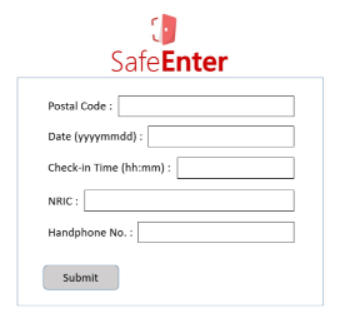
\includegraphics[width=0.25\paperwidth]{C:/Users/Admin/Desktop/Github/question_bank/LyX/static/img/9569-YIJC-2020-P2-Q4-2}
\par\end{center}

\noindent \begin{center}
Check-In Form
\par\end{center}

\subsection*{Task 4.2}

Write program code, \texttt{server.py}, for the back-end server to
display the Check-In form on the clients\textquoteright{} browser
when they scan a QR-code which links to the SafeEnter website. The
server script should include a route \textquoteleft \texttt{/checkin}\textquoteright{}
to receive the inputs from the client, the program code should: 
\begin{itemize}
\item prevent the user from accessing the \textquoteleft \texttt{/checkin}\textquoteright{}
route directly 
\item receive all the inputs in the Check-In form
\item reject empty or null inputs
\item append the new entry into the \texttt{event} table in the given database
\texttt{covid.db }
\item reply by sending a \texttt{checkout.html} page back to the client\textquoteright s
browser, displaying the following Check-Out form, which is to be used
when leaving the venue (Use the picture \texttt{OUT.JPG} provided.)\texttt{
}\hfill{}{[}12{]}
\end{itemize}
\begin{center}
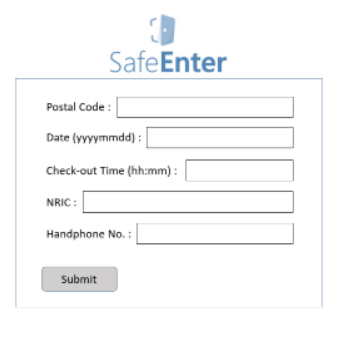
\includegraphics[width=0.25\paperwidth]{C:/Users/Admin/Desktop/Github/question_bank/LyX/static/img/9569-YIJC-2020-P2-Q4-3}
\par\end{center}

\noindent \begin{center}
Check-Out Form
\par\end{center}

\subsection*{Task 4.3}

Modify the program code, \texttt{server.py}, and include an additional
route \textquoteleft \texttt{/checkout}\textquoteright{} to receive
the inputs from the client\textquoteright s Check-Out form when they
leave the venue. The program code should: 
\begin{itemize}
\item allow the user from accessing the \textquoteleft /checkout\textquoteright{}
route directly 
\item receive all the inputs in the Check-Out form 
\item reject empty or null inputs 
\item update the corresponding entry in the \texttt{event} table in the
\textbf{given} database \texttt{covid.db }\hfill{}{[}8{]}
\end{itemize}
Download the files for your program codes for Task 4 as 

\texttt{Task4\_<your name>\_<centre number>\_<index number>\_index.html }

\texttt{Task4\_<your name>\_<centre number>\_<index number>\_checkout.html}

\texttt{Task4\_<your name>\_<centre number>\_<index number>\_server.py }

\texttt{Task4\_<your name>\_<centre number>\_<index number>\_covid.db}

 \newpage 

\item \textbf{{[}ACJC/PRELIM/9569/2021/P1/Q1{]} }

A famous restaurant only accommodates one seating daily from 6.00
pm to 8.00 pm. It has 10 tables, each with a maximum capacity between
2 and 8 people. Advanced reservation is required to dine in at the
restaurant. 

The owner of the restaurant decides to write a program to handle reservations.
As a trial, it can only take a booking for one evening only. 

A procedure to initialise the arrays \texttt{MaxSize}, \texttt{IsBooked}
and \texttt{GroupSize} has been defined. The indexes of each array
corresponds to the table number.

\begin{tabular}{|c|c|}
\multicolumn{1}{c}{Index} & \multicolumn{1}{c}{\texttt{MaxSize}}\tabularnewline
\hline 
1 & 2\tabularnewline
\hline 
2 & 2\tabularnewline
\hline 
3 & 4\tabularnewline
\hline 
4 & 4\tabularnewline
\hline 
5 & 4\tabularnewline
\hline 
6 & 6\tabularnewline
\hline 
7 & 6\tabularnewline
\hline 
8 & 6\tabularnewline
\hline 
9 & 8\tabularnewline
\hline 
10 & 8\tabularnewline
\hline 
\end{tabular}%
\begin{tabular}{|c|c|}
\multicolumn{1}{c}{} & \multicolumn{1}{c}{\texttt{IsBooked}}\tabularnewline
\hline 
1 & FALSE\tabularnewline
\hline 
2 & FALSE\tabularnewline
\hline 
3 & FALSE\tabularnewline
\hline 
4 & FALSE\tabularnewline
\hline 
5 & FALSE\tabularnewline
\hline 
6 & FALSE\tabularnewline
\hline 
7 & FALSE\tabularnewline
\hline 
8 & FALSE\tabularnewline
\hline 
9 & FALSE\tabularnewline
\hline 
10 & FALSE\tabularnewline
\hline 
\end{tabular}%
\begin{tabular}{|c|c|}
\multicolumn{1}{c}{} & \multicolumn{1}{c}{\texttt{GroupSize}}\tabularnewline
\hline 
1 & \tabularnewline
\hline 
2 & \tabularnewline
\hline 
3 & \tabularnewline
\hline 
4 & \tabularnewline
\hline 
5 & \tabularnewline
\hline 
6 & \tabularnewline
\hline 
7 & \tabularnewline
\hline 
8 & \tabularnewline
\hline 
9 & \tabularnewline
\hline 
10 & \tabularnewline
\hline 
\end{tabular}

The procedure \texttt{BookTable} is shown below. When a booking enquiry
is made, the number of customers is keyed in. 

\fbox{\begin{minipage}[t]{0.8\columnwidth}%
\texttt{01 PROCEDURE BookTable }

\texttt{02 \qquad{}DECLARE NumberOfCustomers, TableNumber : INTEGERS }

\texttt{03 \qquad{}DECLARE Found : BOOLEAN}

\texttt{04 \qquad{}INPUT NumberOfCustomers }

\texttt{05 \qquad{}TableNumber \textleftarrow{} 0 }

\texttt{06 \qquad{}FOUND \textleftarrow{} False }

\texttt{07 \qquad{}REPEAT }

\texttt{08 \qquad{}\qquad{}TableNumber \textleftarrow{} TableNumber
+ 1 }

\texttt{09 \qquad{}\qquad{}IF MaxSize{[}TableNumber{]} > NumberOfCustomers
AND IsBooked{[}TableNumber{]} = FALSE }

\texttt{10 \qquad{}\qquad{}\qquad{}THEN }

\texttt{11 \qquad{}\qquad{}\qquad{}\qquad{}Found \textleftarrow{}
TRUE }

\texttt{12 \qquad{}\qquad{}ENDIF }

\texttt{13 \qquad{}UNTIL Found = TRUE AND TableNumber = 10 }

\texttt{14 \qquad{}\qquad{}IF Found = FALSE }

\texttt{15 \qquad{}\qquad{}\qquad{}THEN }

\texttt{16 \qquad{}\qquad{}\qquad{}OUTPUT \textquotedbl No tables
with enough seats available.\textquotedbl{} }

\texttt{17 \qquad{}\qquad{}\qquad{}ELSE }

\texttt{18 \qquad{}\qquad{}\qquad{}\qquad{}GroupSize{[}TableNumber{]}
\textleftarrow{} NumberOfCustomers }

\texttt{19 \qquad{}\qquad{}\qquad{}\qquad{}OUTPUT \textquotedbl Booking
is successful! Table no:\textquotedbl , TableNumber }

\texttt{20 \qquad{}ENDIF }

\texttt{21 ENDPROCEDURE}%
\end{minipage}}
\begin{enumerate}
\item There are two errors and one missing line of code in the procedure
above.
\begin{enumerate}
\item Name the type of the errors. \hfill{}{[}1{]}
\item Describe the errors and the changes required to correct them. \hfill{}{[}3{]}
\item Write the missing line of code and state where it should be located.
\hfill{}{[}2{]}
\end{enumerate}
\item Once the procedure \texttt{BookTable} is able to run correctly, the
owner decides to improve its functionality.

The procedure should ask the user to input the name and the mobile
number of the person making the reservation when a table with enough
seats can be found.

Name and describe two data validation techniques that can be applied
to any of the inputs mentioned above.\hfill{} {[}2{]}
\item Explain the difference in the type of memory allocation for an array
and a linked list. \hfill{}{[}2{]}
\end{enumerate}

 \newpage 

\item \textbf{{[}ACJC/PRELIM/9569/2021/P1/Q2{]} }

A hash table has 8 spaces to store strings, indexed from 1 to 8 inclusive.

The hash function finds the ASCII number of the first letter of the
string, then counts the number of 1s in its binary representation.
This is the index in which the string will be inserted into the hash
table.

For example, the string \texttt{'Arlington'} will have index 2 because
the ASCII number of '\texttt{A}' is 65, which is \texttt{1000001}
in binary, and there are two \texttt{1}s.

The following strings are to be inserted into the hash table in the
order given.

\texttt{'Grover', }

\texttt{Horsburgh', }

\texttt{'Island',}

\texttt{'Jordan', }

\texttt{'Kalman'}
\begin{enumerate}
\item Find the output of the hash function for each of the strings. \hfill{}{[}5{]}
\item {}
\begin{enumerate}
\item Suppose collisions in the hash table are to be resolved using open
hashing.

Draw the hash table after all five strings are inserted. \hfill{}{[}5{]}
\item Suppose instead that collisions in the hash table are to be resolved
using closed hashing, where spaces 6 to 8 (inclusive) are used as
the overflow storage.

Draw the hash table after all five strings are inserted. \hfill{}
{[}2{]}
\end{enumerate}
\item Explain why the space with index 1 in the hash table will never be
occupied unless there is a collision. \hfill{} {[}2{]}
\end{enumerate}

 \newpage 

\item \textbf{{[}ACJC/PRELIM/9569/2021/P1/Q3{]} }

The diagram below shows a flowchart for performing a search through
a binary tree. The algorithm searches through \texttt{Tree} for \texttt{Searchfor}.
If it finds a node whose data is equal to \texttt{Searchfor}, it outputs
\texttt{Found}. Otherwise, it outputs \texttt{Not Found}.
\noindent \begin{center}
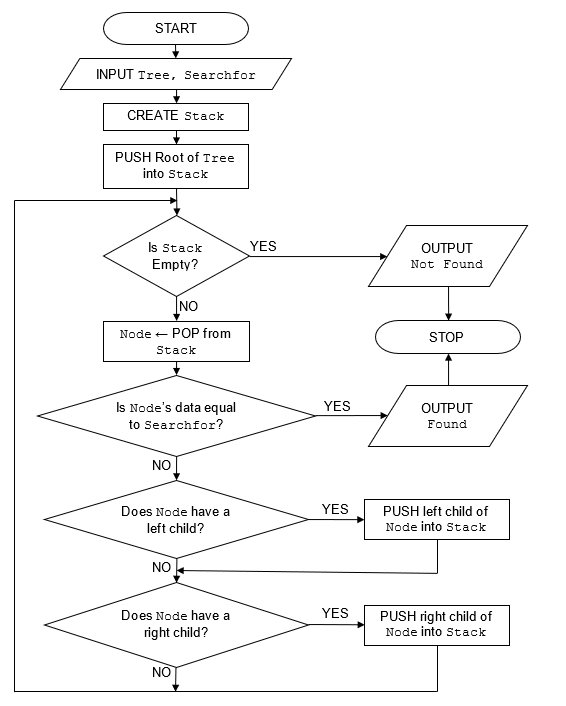
\includegraphics[scale=0.8]{C:/Users/Admin/Desktop/Github/question_bank/LyX/static/img/9569-ACJC-2021-P1-Q3-1}\quad{}
\par\end{center}
\begin{enumerate}
\item Given the input \texttt{Tree} below and a \texttt{Searchfor} value
of 5, draw a trace table to illustrate the algorithm. \hfill{} {[}5{]}
\noindent \begin{center}
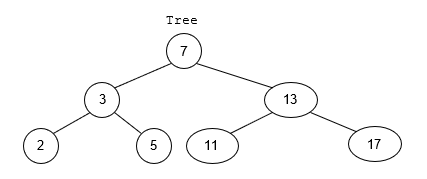
\includegraphics[scale=0.8]{C:/Users/Admin/Desktop/Github/question_bank/LyX/static/img/9569-ACJC-2021-P1-Q3-2}\quad{}
\par\end{center}
\item State whether this is a depth-first search or a breadth-first search.
\hfill{} {[}1{]}
\item Draw a flowchart to illustrate how the other kind of search in (ii)
can be carried out using the same input parameters. \hfill{} {[}3{]}
\item Given the same input \texttt{Tree} and the same \texttt{Searchfo}r
value of 5, draw a trace table to illustrate the algorithm in (iii).
\hfill{} {[}5{]}
\end{enumerate}

 \newpage 

\item \textbf{{[}ACJC/PRELIM/9569/2021/P1/Q4{]} }

Merge sort and bubble sort are two sorting algorithms that can be
applied to sort a list of integers in ascending order.
\begin{enumerate}
\item By briefly comparing the operation of merge sort and bubble sort,
state which algorithm would be more efficient. \hfill{}{[}3{]}
\end{enumerate}
The pseudocode for the recursive \texttt{MergeSortDesc} function is
shown below, which takes in a list of integers and returns a new list
with the integers sorted in descending order. It makes use of the
\texttt{MergeDesc} function in line \texttt{10} that merges two lists
of integers sorted in descending order into a single list of integers
sorted in descending order as well.

\fbox{\begin{minipage}[t]{0.8\columnwidth}%
\texttt{01 FUNCTION MergeSortDesc(MyList: LIST) RETURNS LIST }

\texttt{02 \qquad{}MaxIndex \textleftarrow{} LENGTH(MyList) }

\texttt{03 \qquad{}\qquad{}IF ......A...... }

\texttt{04 \qquad{}\qquad{}\qquad{}THEN }

\texttt{05 \qquad{}\qquad{}\qquad{}Half \textleftarrow{} ......B...... }

\texttt{06 \qquad{}\qquad{}\qquad{}LeftList \textleftarrow{} LEFT(MyList,
Half) }

\texttt{07 \qquad{}\qquad{}\qquad{}RightList \textleftarrow{} RIGHT(MyList,
Half) }

\texttt{08 \qquad{}\qquad{}\qquad{}SortedLeftList \textleftarrow{}
MergeSortDesc(LeftList) }

\texttt{09 \qquad{}\qquad{}\qquad{}SortedRightList \textleftarrow{}
MergeSortDesc(RightList) }

\texttt{10 \qquad{}\qquad{}\qquad{}Result \textleftarrow{} MergeDesc(SortedLeftList,
SortedRightList) }

\texttt{11 \qquad{}\qquad{}ELSE }

\texttt{12 \qquad{}\qquad{}\qquad{}......C...... }

\texttt{13 \qquad{}\qquad{}ENDIF }

\texttt{14 \qquad{}\qquad{}RETURN Result }

\texttt{15 ENDFUNCTION}%
\end{minipage}}
\begin{enumerate}
\item[(b)] State what is meant by a \textbf{recursive} function. \hfill{}{[}2{]}
\item[(c)] Write the pseudocode for \texttt{A}, \texttt{B} and \texttt{C} in
the algorithm. \hfill{}{[}3{]}
\item[(d)] Describe the operation of the \texttt{MergeDesc} function.

Assume that the function does not modify the two input lists.\hfill{}
{[}4{]}
\end{enumerate}

 \newpage 

\item \textbf{{[}ACJC/PRELIM/9569/2021/P1/Q5{]} }

A gym organises various classes and runs a loyalty membership programme
with four tiers: Bronze, Silver, Gold and Diamond 

Upon joining, each member is given a unique membership number and
starts with a Bronze membership. Each member can sign up for multiple
classes at a reduced rate based on the membership tier.

Each class has a unique class name. Some classes are offered at three
different levels: Beginner, Intermediate and Advanced

Each instructor is identified with a unique three-character code and
can take one or more classes.

A relational database is to be created to store data about members,
employees and classes.

Part of the table \texttt{MEMBER}, which is a first attempt at the
database design, is shown below. 

\begin{tabular}{|c|c|c|c|c|}
\hline 
MemberNo  & MemberName  & MemberTier  & ClassName & InstCode\tabularnewline
\hline 
\multirow{3}{*}{5 } & \multirow{3}{*}{Lindy White} & \multirow{3}{*}{Silver } & Body Pump  & WAY \tabularnewline
\cline{4-5} \cline{5-5} 
 &  &  & Yoga (Beginner)  & DAV \tabularnewline
\cline{4-5} \cline{5-5} 
 &  &  & Zumba & ROG\tabularnewline
\hline 
\dots{}  & \dots{}  & \dots{}  & \dots{}  & ...\tabularnewline
\hline 
78  & Derek Davis  & Bronze  & Muay Thai (Beginner)  & CHA \tabularnewline
\hline 
\dots{} & \dots{}  & \dots{} \dots{} \dots{}  & \dots{}  & ...\tabularnewline
\hline 
\multirow{4}{*}{132} & \multirow{4}{*}{John Chua } & \multirow{4}{*}{Diamond } & Circuits (Intermediate)  & JON \tabularnewline
\cline{4-5} \cline{5-5} 
 &  &  & Muay Thai (Intermediate)  & LEX \tabularnewline
\cline{4-5} \cline{5-5} 
 &  &  & Yoga (Advanced) & DAV \tabularnewline
\cline{4-5} \cline{5-5} 
 &  &  & Zumba & ROG\tabularnewline
\hline 
\dots{}  & \dots{} & \dots{}  & \dots{}  & \dots{}\tabularnewline
\hline 
\end{tabular}
\begin{enumerate}
\item The table \texttt{MEMBER} is not normalised.
\begin{enumerate}
\item Describe \textbf{one} potential issue that may be encountered when
the data are maintained in such a non-normalised table. \hfill{}{[}1{]}
\item Explain why the table is not in first normal form (1NF). \hfill{}{[}1{]}
\end{enumerate}
\item A second attempt at the database design gives rise to two tables:

\texttt{MEMBER(MemberNo, MemberName, MemberTier)}

\texttt{MEMBERCLASSES(MemberNo, ClassName, Instructor)}

The primary keys are not shown. 
\begin{enumerate}
\item State what is meant by a \textbf{primary key}. \hfill{}{[}1{]}
\item By referring to the relationship between the tables \texttt{MEMBER}
and \texttt{MEMBERCLASSES}, state how the relationship is implemented.\hfill{}
{[}2{]}
\item Write an SQL query to create the table MEMBER with the appropriate
constraints.\hfill{} {[}4{]}
\end{enumerate}
\item Another attempt at the database design needs to be made to ensure
that all the tables are in third normal form (3NF). 

In addition, the following data need to be recorded in the database:
\begin{itemize}
\item the date on which each member signs up for the gym membership; 
\item the attendance of each member in any classes taken;
\item the original fee, i.e. before discount, of each class; 
\item the name and the salary of each instructor. 
\end{itemize}
\begin{enumerate}
\item State the total number of 3NF tables required and give their names.
\hfill{}{[}1{]}
\item Draw the Entity-Relationship (E-R) diagram to show the 3NF tables
and the relationships between them. \hfill{}{[}4{]}
\item A table description can be written as:

\texttt{TableName(}\texttt{\uline{Attribute1}}\texttt{, Attribute2{*},
Attribute3, ...) }

The primary key is indicated by underlining one or more attributes.
Foreign keys are indicated by using a dashed underline/asterisk. 

Using the information provided, write table descriptions for all the
3NF tables you identified in \textbf{(c)(i)}.\hfill{} {[}8{]}
\end{enumerate}
\item Making backups and archives are performed to prevent the loss of data.

Explain the difference between a backup and an archive.\hfill{} {[}2{]}
\end{enumerate}

 \newpage 

\item \textbf{{[}ACJC/PRELIM/9569/2021/P1/Q6{]} }

A driving simulator is programmed using Object-Oriented Programming
(OOP).

The diagram below shows a UML Class Diagram with \textbf{some} of
the classes, attributes, and methods used in the simulator.
\noindent \begin{center}
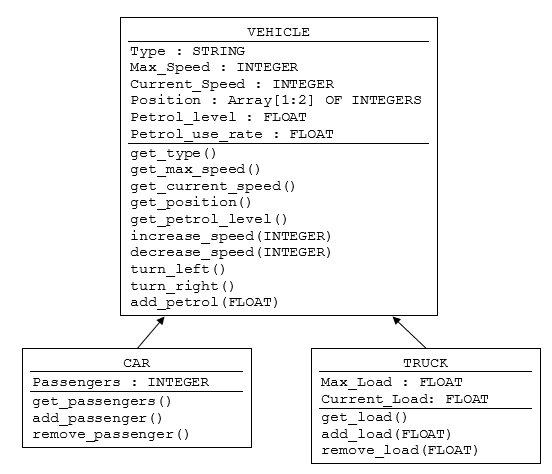
\includegraphics[scale=0.8]{C:/Users/Admin/Desktop/Github/question_bank/LyX/static/img/9569-ACJC-2021-P1-Q6}\quad{}
\par\end{center}
\begin{enumerate}
\item State the relationship between the \texttt{CAR} class and the \texttt{VEHICLE}
class. \hfill{}{[}1{]}
\item Explain briefly, in this context, how each of the following features
of Object-Oriented Programming help the simulation to be developed
more efficiently.
\begin{enumerate}
\item Abstraction \hfill{} {[}2{]}
\item Inheritance \hfill{}{[}2{]}
\end{enumerate}
\item The petrol use rate depends on the speed at which the vehicle is travelling,
as well as the mass of the vehicle and the contents of the vehicle
-- the number of passengers in a car, or the mass of the load in
a truck. Explain how polymorphism can be used in this case to write
the simulation. \hfill{}{[}2{]}
\end{enumerate}

 \newpage 

\item \textbf{{[}ACJC/PRELIM/9569/2021/P1/Q7{]} }

A new social media platform is to be created. In years to come, it
is expected to be as popular globally as other trending social media
platforms.
\begin{enumerate}
\item Give two reasons why a NoSQL database is likely to be more suitable
than an SQL database for the social media platform. \hfill{}{[}2{]}
\end{enumerate}
A basic login page that controls access to user accounts is shown
below. The password field masks the user input with a dot (\textbullet )
replacing each of the characters supplied.
\noindent \begin{center}
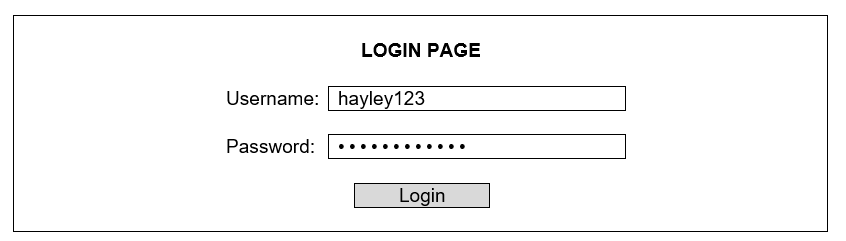
\includegraphics[scale=0.5]{C:/Users/Admin/Desktop/Github/question_bank/LyX/static/img/9569-ACJC-2021-P1-Q7}\quad{}
\par\end{center}
\begin{enumerate}
\item[(b)] When the login button is clicked, the program processes the username
and password supplied by the user.

It displays an error message if the username entered does not exist
in the database. If the password entered matches the registered password
for the username, login is granted. Otherwise, the program displays
an error message to indicate the user of the incorrect password entered.

The account will be locked if the user enters the correct username,
but enters the wrong password three times.
\begin{enumerate}
\item Create a decision table to show these conditions and actions. \hfill{}{[}4{]} 
\item Simplify your decision table by removing redundancies. \hfill{}{[}1{]} 
\end{enumerate}
\item[(c)] It is known that users tend to have different problems associated
with passwords.

Besides the error message to tell the user when an incorrect password
is entered, describe \textbf{two} examples based on usability principles
that can be applied to improve the functionality of the login page.
{[}2{]}
\item[(d)] Explain why the HTTP POST method should be used instead of the HTTP
GET method for the login request. \hfill{}{[}2{]}
\end{enumerate}

 \newpage 

\item \textbf{{[}ACJC/PRELIM/9569/2021/P1/Q8{]} }

In a hypothetical scenario, a data security company is helping a client
company manage a database of the client company\textquoteright s customers.
The data security company notices a possible vulnerability in the
database.

Further investigation shows that the vulnerability is obscure and
that none or few of the programmers anticipated it. Since the vulnerability
is obscure, they determine that the chances of the database being
breached are minimal, and decide not to tell the client company about
it. 

Instead, the data security company waits until the next time the database
is due for scheduled maintenance to attempt to fix the vulnerability.
By doing so, they can give themselves enough time to learn how to
fix the vulnerability and avoid causing unnecessary panic within the
client company or among the customers, which could lead to a potential
loss of business.

Describe how each of the following ethical guidelines was breached
by the data security company.
\begin{enumerate}
\item Integrity \hfill{}{[}2{]}
\item Responsibility \hfill{}{[}2{]}
\item Competence \hfill{}{[}2{]}
\item Professionalism \hfill{}{[}2{]}
\end{enumerate}

 \newpage 

\item \textbf{{[}ACJC/PRELIM/9569/2021/P2/Q1{]} }

\noindent The Universal Product Code (UPC) system is used for tracking
trade items in shipping, inventory, and sales. Each item is given
a 12-digit identification number. The validity of this identification
number can be checked using a checksum. If $x_{i}$ represents the
$i$th digit (starting with $i=1$ as the leftmost digit), then a
valid identification number satisfies the condition that

\noindent 
\[
3x_{1}+x_{2}+3x_{3}+x_{4}+3x_{5}+x_{6}+3x_{7}+x_{8}+3x_{9}+x_{10}+3x_{11}+x_{12}
\]

\noindent has a remainder of 0 when divided by 10.

\noindent The identification number can be encoded into a barcode.
For this Task, the barcode will be represented as a string of '\texttt{0}'s
and '\texttt{1}'s, where '\texttt{0}' represents a white stripe and
'\texttt{1}' represents a black stripe.

\noindent The barcode is divided into seven sections. From left to
right, they are
\begin{itemize}
\item A \textquoteleft quiet zone\textquoteright{} consisting of nine '\texttt{0}'s; 
\item A start pattern which is always '\texttt{101}'; 
\item The first six digits of the identification number are encoded using
the table below; 
\item A middle pattern which is always '\texttt{01010}'; 
\item The last six digits of the identification number are encoded using
the table below; 
\item An end pattern which is always '\texttt{101}'; 
\item A \textquoteleft quiet zone\textquoteright{} consisting of nine '\texttt{0}'s.
\end{itemize}
\noindent The table below shows the encoding system for the digits.
Note that depending on whether the digit occurs in the first six digits
or the last six digits, it would be encoded differently. However,
the two encodings are optical inverses of each other -- a '\texttt{0}'
is changed into a '\texttt{1}', and vice versa.
\noindent \begin{center}
\begin{tabular}{|c|c|c|}
\hline 
Digit  & First six digits & Last six digits\tabularnewline
\hline 
0  & \texttt{'0001101' } & \texttt{'1110010'}\tabularnewline
\hline 
1  & \texttt{'0011001' } & \texttt{'1100110'}\tabularnewline
\hline 
2  & \texttt{'0010011'} & \texttt{'1101100'}\tabularnewline
\hline 
3  & \texttt{'0111101' } & \texttt{'1000010' }\tabularnewline
\hline 
4  & \texttt{'0100011' } & \texttt{'1011100' }\tabularnewline
\hline 
5  & \texttt{'0110001' } & \texttt{'1001110'}\tabularnewline
\hline 
6  & \texttt{'0101111' } & \texttt{'1010000'}\tabularnewline
\hline 
7  & \texttt{'0111011'} & \texttt{'1000100' }\tabularnewline
\hline 
8  & \texttt{'0110111' } & \texttt{'1001000'}\tabularnewline
\hline 
9  & \texttt{'0001011' } & \texttt{'1110100'}\tabularnewline
\hline 
\end{tabular}
\par\end{center}

\noindent The reason for encoding the first and last six digits differently
is that the barcode may inadvertently be scanned upside down. Notice
that in the first six digits, the encoding for each digit contains
an odd number of '\texttt{1}'s, while in the last six digits, the
encoding for each digit contains an even number of '\texttt{1}'s.
This allows the scanning software to detect if the barcode has been
placed upside down and correct it. \quad{} 

\noindent For example, the UPC identification number 036000 291452
would be encoded as:

\begin{tabular}{|c|c|c|c|c|c|}
\hline 
000000000 & 101 & 0001101 & 0111101 & 0101111 & 0001101\tabularnewline
\hline 
Quiet & Start & 0 & 3  & 6  & 0\tabularnewline
\hline 
\end{tabular}

\begin{tabular}{|c|c|c|c|c|c|}
\hline 
0001101  & 0001101  & 01010 & 1101100  & 1110100  & 1100110\tabularnewline
\hline 
0  & 0  & Middle & 2  & 9  & 1\tabularnewline
\hline 
\end{tabular}

\begin{tabular}{|c|c|c|c|c|}
\hline 
1011100 & 1001110  & 1101100  & 101 & 000000000 \tabularnewline
\hline 
4  & 5  & 2  & End & Quiet\tabularnewline
\hline 
\end{tabular}
\noindent \begin{center}
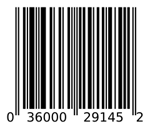
\includegraphics[scale=0.8]{C:/Users/Admin/Desktop/Github/question_bank/LyX/static/img/9569-ACJC-2021-P2-Q1}
\par\end{center}

\noindent (Notice that in an actual barcode, the stripes for the start,
middle and end pattern are usually slightly longer than the surrounding
stripes. This is to help humans to read it.)

\subsection*{Task 1.1}

\noindent Write a function to determine the validity of any input
string as an identification number. \hfill{}{[}5{]}

\subsection*{Task 1.2}

\noindent Write a function to convert a valid identification number,
given as a string, into a barcode (a string of '\texttt{0}'s and '\texttt{1}'s).
\hfill{}{[}5{]}

\subsection*{Task 1.3}

\noindent Write a function that takes in a string, check whether it
represents a valid barcode, and converts it to an identification number
if it does. Note that the barcode may be upside down. \hfill{}{[}11{]}

\noindent Download your program code and output for Task 1 as \texttt{TASK1\_<your
name>\_<centre number>\_<index number>.ipynb}

 \newpage 

\item \textbf{{[}ACJC/PRELIM/9569/2021/P2/Q2{]} }

\noindent A file compression algorithm reduces file sizes so that
files can be sent more quickly. One such algorithm is the Huffman
algorithm for text files, which will be implemented in this task.

\noindent Unlike ASCII, which assigns a fixed size of 8 bits for each
character, the Huffman algorithm assigns fewer bits to more common
characters and more bits to less common characters. For example, in
a long text written in English, characters such as '\texttt{e}' and
'\texttt{t}' will have fewer bits assigned to them than characters
such as '\texttt{q}' and '\texttt{z}'. If the text is long enough,
this will use fewer bits in total to encode the text compared to ASCII.

\noindent To know which sequence of bits to encode for each character,
the \textbf{frequency} of each character, which is the number of times
each character appears in the text file, is tabulated.

\noindent The characters are put into a tree. A node is created for
each character. The following steps are then repeated until there
is only one node without a parent:
\begin{enumerate}
\item Identify the two nodes, without parents, which have the lowest frequency. 
\item Create a new node whose left and right children are the two nodes
identified in Step 1. The frequency of the new node is the total of
the frequency of its children.
\end{enumerate}
\noindent The diagram on the following page shows the process of creation
of a tree for a file with only five distinct characters ('\texttt{A}',
'\texttt{E}', '\texttt{I}', '\texttt{O}' and '\texttt{U}'), in five
stages.

\noindent The bit sequence assigned to a character will be the path
from the root to the node corresponding to that character, where going
left corresponds to '\texttt{0}' and going right corresponds to '\texttt{1}'.
For example, '\texttt{A}' is encoded as '\texttt{10}' and '\texttt{O}'
is encoded as '\texttt{011}'.

\subsection*{Task 2.1}

\noindent Create a Node class that has the following attributes: 
\begin{itemize}
\item \texttt{data}, which is determined when the node is initialized 
\item \texttt{left}, a pointer to another node, 
\item \texttt{right}, a pointer to another node 
\end{itemize}
\noindent When the node is initialised, left and right do not point
to anything. The class also has setter methods for left and right,
and getter methods for all three attributes. \hfill{}{[}3{]}

\subsection*{Task 2.2}

\noindent Write code that takes an input \texttt{.txt} file and creates
a dictionary whose keys are the characters in the file, including
spaces, punctuation and line breaks ('\texttt{\textbackslash n}'),
and the value of a key is its frequency in the file. Uppercase and
lowercase letters should be considered as different characters.

\noindent Create a node for each character in the file, and put the
nodes into a list in ascending order of frequency. \hfill{}{[}11{]}

\subsection*{Task 2.3}

\noindent Create a tree using the algorithm described above. \hfill{}{[}5{]}

\subsection*{Task 2.4}

\noindent Create a dictionary whose keys are the characters, and the
value of a key is the bit sequence of that character, expressed as
a string of '\texttt{0}'s and '\texttt{1}'s.

\noindent Carry out Tasks 2.2 to 2.4 on the file \texttt{HAMLET.txt}.
Compress the file by replacing each character with its bit sequence
and writing the output to a new file, \texttt{HAMLET\_compressed.txt}.
{[}8{]}

\noindent Download your program code and output for Task 2 as \texttt{TASK2\_<your
name>\_<centre number>\_<index number>.ipynb} 

\noindent Diagram showing how the tree is created based on the frequency
of each character: 
\noindent \begin{center}
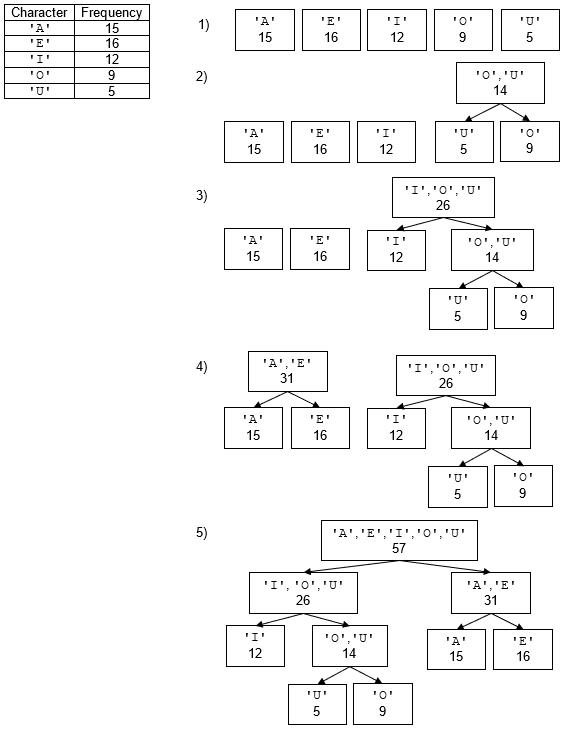
\includegraphics[scale=0.8]{C:/Users/Admin/Desktop/Github/question_bank/LyX/static/img/9569-ACJC-2021-P2-Q2}\quad{}
\par\end{center}

 \newpage 

\item \textbf{{[}ACJC/PRELIM/9569/2021/P2/Q3{]} }

\noindent A community centre is required to keep COVID-19 vaccination
records of its members in a NoSQL database. The CoviDie vaccine, which
requires two doses to be taken at least 21 days apart, has been secured
for all members of this particular community centre. 

\noindent As everyone needs to be vaccinated before the end of 2021,
we shall only consider the year 2021, which is a non-leap year. The
table below shows the number of days available in the twelve months
of 2021.
\noindent \begin{center}
\begin{tabular}{|c|c|c|c|c|c|c|}
\hline 
Month  & 01  & 02  & 03  & 04  & 05  & 06\tabularnewline
\hline 
Days  & 31  & 28  & 31  & 30  & 31 & 30\tabularnewline
\hline 
\end{tabular}
\par\end{center}

\noindent \begin{center}
\begin{tabular}{|c|c|c|c|c|c|c|}
\hline 
Month  & 07  & 08  & 09 & 10  & 11  & 12\tabularnewline
\hline 
Days & 31 & 31 & 30 & 31 & 30 & 31\tabularnewline
\hline 
\end{tabular}
\par\end{center}

\subsection*{Task 3.1}

\noindent Write a function \texttt{second\_dose\_date(date)} that:
\begin{itemize}
\item Takes a string value \texttt{date} in the format \texttt{YYYYMMDD},
where \texttt{YYYY} represents the year, \texttt{MM} represents the
month and \texttt{DD} represents the day 
\item determines the date that is 21 days after the input date 
\item returns the result date in the format \texttt{YYYYMMDD}
\end{itemize}
\noindent Assume that the result date does not go beyond \texttt{20211231}.
\hfill{}{[}3{]}

\noindent Test the function using the following three calls:
\begin{itemize}
\item \texttt{second\_dose\_date('20210105') }
\item \texttt{second\_dose\_date('20210212') }
\item \texttt{second\_dose\_date('20210919')} \hfill{}{[}3{]}
\end{itemize}
\noindent Save your program code as

\noindent \texttt{TASK3\_1\_<your name>\_<centre number>\_<index number>.py}

\subsection*{Task 3.2}

\noindent The list of members under the management committee of the
community centre is stored in the text file \texttt{VACCINATION.txt}.
Some members have not taken the vaccination at all, some others have
only taken the first dose, while the rest have taken both doses.

\noindent Each line of the text file is of the following format: \texttt{\_id,name,date\_first\_dose,date\_second\_dose,remarks}
\begin{itemize}
\item \texttt{\_id} is a unique integer ID assigned to the member 
\item \texttt{name} is the name of the member 
\item \texttt{date\_first\_dose} and \texttt{date\_second\_dose}, if any,
represent the date of the first dose and the date of the second dose
respectively in the format \texttt{YYYYMMDD} 
\item \texttt{remarks}, if any, shows the pre-existing condition of the
member
\end{itemize}
\noindent Write program code to insert the data from \texttt{VACCINATION.txt}
into a NoSQL database \texttt{community\_centre} under the collection
\texttt{management\_committee}. The program should clear the collection
\texttt{management\_committee} if it exists inside the database. \hfill{}{[}7{]}

\noindent Save your program code as T\texttt{ASK3\_2\_<your name>\_<centre
number>\_<index number>.py}

\subsection*{Task 3.3}

\noindent The community centre needs a program to check the vaccination
status of its members. The program should also allow for the downloading
of vaccination certificates for members who are fully vaccinated,
i.e. they have taken the two doses.

\noindent Write program code to: 
\begin{itemize}
\item prompt the user to input a member ID, and keep prompting until the
user keys in numeric character(s) 
\item if the member ID is available in the NoSQL database, perform either
one of the following: 
\begin{itemize}
\item if the member is fully vaccinated, write the vaccination certificate
to an output text file and update the record in the NoSQL database
by including a field and an appropriate value to indicate that the
certificate has been downloaded 
\item if the member has only taken the first dose, output a message to show
the date from which the member can take the second dose 
\item if the member has not taken the vaccination at all, output a message
to tell that the member should take the first dose as soon as possible 
\end{itemize}
\item otherwise, if the member ID is not available in the NoSQL database,
display an appropriate message and terminate the program
\end{itemize}
\noindent The format of the vaccination certificate is as follows.

\noindent \texttt{VACCINATION CERTIFICATE}

\noindent \texttt{Name: <name> }

\noindent \texttt{Vaccine type: CoviDie }

\noindent \texttt{Date of first dose: <date\_first\_dose> }

\noindent \texttt{Date of second dose: <date\_second\_dose>} \hfill{}{[}8{]}

\noindent Save your program code as \texttt{TASK3\_3\_<your name>\_<centre
number>\_<index number>.py}

\noindent Test your program for the member with \texttt{member\_id
= 24}. \hfill{}{[}2{]}

\noindent The output text file should be saved as \texttt{TASK3\_3\_<your
name>\_<centre number>\_<index number>.txt}

 \newpage 

\item \textbf{{[}ACJC/PRELIM/9569/2021/P2/Q4{]} }

\noindent A company specialising in bento boxes wishes to trial a
relational database management system to manage its data. It is expected
that the database should be normalised to third normal form (3NF).

\noindent The company owns four kiosks. For each of the kiosks, the
following information is to be recorded in the table \texttt{Kiosk}: 
\begin{itemize}
\item \texttt{KioskID} -- the unique integer assigned to the kiosk 
\item \texttt{Location} -- the area where the kiosk is located 
\item \texttt{Rating} -- the average rating of the kiosk between 0.0 and
5.0 inclusive
\end{itemize}
\noindent The company offers eight different types of bento boxes.
Some of them may contain egg, nut, seafood or a combination of them.
For each of the bento boxes, the following information is to be recorded
in the table \texttt{BentoBox}:
\begin{itemize}
\item \texttt{BentoName} -- the unique name of the bento box 
\item \texttt{ProductionCost} -- the cost incurred in producing the bento
box in dollars and cents 
\item \texttt{ContainEgg} -- an integer 0 for not containing egg and 1
for containing egg 
\item \texttt{ContainNut} -- an integer 0 for not containing nut and 1
for containing nut 
\item \texttt{ContainSeafood} -- an integer 0 for not containing seafood
and 1 for containing seafood 
\end{itemize}
\noindent Each of the four kiosks sells all eight bento boxes at different
mark-up prices. Another table \texttt{KioskBento} is needed to record
the following information:
\begin{itemize}
\item \texttt{KioskID} -- the unique integer assigned to the kiosk 
\item \texttt{BentoName} -- the unique name of the bento box 
\item \texttt{SellPrice} -- the price at which the bento box is sold at
the kiosk in dollars and cents
\end{itemize}

\subsection*{Task 4.1}

\noindent Create an SQL file called \texttt{TASK4\_1\_<your name>\_<centre
number>\_<index number>.sql} to show the SQL code to create the database
\texttt{bento\_company.db} with the three tables. \hfill{}{[}5{]}

\noindent Save your SQL code as \texttt{TASK4\_1\_<your name>\_<centre
number>\_<index number>.sql}

\subsection*{Task 4.2}

\noindent The files \texttt{KIOSK.txt} and \texttt{BENTOBOX.txt} contain
information about the company\textquoteright s kiosks and bento boxes
respectively for insertion into the database. Each row in the two
files is a comma-separated list of information. 

\noindent For \texttt{KIOSK.txt}, information about each kiosk is
given in the following order: \texttt{KioskID}, \texttt{location},
\texttt{rating}

\noindent For \texttt{BENTOBOX.txt}, information about each bento
box is given in the following order: \texttt{BentoName}, \texttt{ProductionCost},
\texttt{ContainEgg}, \texttt{ContainNut}, \texttt{ContainSeafood}

\noindent The mark-up price for each kiosk has been set as follows:
\begin{itemize}
\item \texttt{KioskID = 1} sells each bento box at a price that is \$2.60
higher than the production cost
\item \texttt{KioskID = 2} sells each bento box at a price that is \$2.90
higher than the production cost 
\item \texttt{KioskID = 3} sells each bento box at a price that is \$2.40
higher than the production cost 
\item \texttt{KioskID = 4} sells each bento box at a price that is \$3.10
higher than the production cost
\end{itemize}
\noindent Write program code to insert all the required information
into the database \texttt{bento\_company.db}. \hfill{}{[}6{]}

\noindent Save your program code as \texttt{TASK4\_2\_<your name>\_<centre
number>\_<index number>.py}

\noindent Run your program.

\subsection*{Task 4.3}

\noindent The company wishes to create a form to display the bento
boxes sold at a particular kiosk and their prices in a web browser.
The form should allow customers to indicate egg, nut and seafood allergies,
if any, and filter out the bento boxes that they cannot consume.

\noindent Write a Python program and the necessary files to create
a web application that:
\begin{itemize}
\item receives input from a HTML form that includes:
\begin{itemize}
\item a text box to enter the \texttt{location} of the kiosk 
\item three checkboxes to indicate egg, nut and seafood allergies, if any
\end{itemize}
\item returns a HTML document to display only the bento boxes that the customers
can consume based on the allergies indicated, if any, and their prices
for the given \texttt{location}
\end{itemize}
\noindent Input validation is not required. \hfill{}{[}10{]}

\noindent Save your Python program as \texttt{TASK4\_3\_<your name>\_<centre
number>\_<index number>.py}

\noindent with any additional files / sub-folders as needed in a folder
named \texttt{TASK4\_3\_<your name>\_<centre number>\_<index number>}

\noindent Run and test the web application using the following input:
\begin{itemize}
\item \texttt{'Woodlands'} entered as the \texttt{location} 
\item checkboxes indicating egg and seafood allergies ticked \hfill{}{[}2{]}
\end{itemize}
\noindent Save the output of the program as \texttt{TASK4\_3\_<your
name>\_<centre number>\_<index number>.html }

 \newpage 

\item \textbf{{[}DHS/PRELIM/9569/2021/P1/Q1{]} }

A cosmic ray striking computer memory at just the right time can flip
a bit, turning a 0 into a 1 or vice versa. 

Bit flips had caused plane accidents, software glitches, and at times,
the Blue Screen of Death (BSoD) on personal computers. 
\begin{enumerate}
\item The hexadecimal number \texttt{D4} had been changed to \texttt{9A}.
Suggest the minimum number of times a bit flip could have affected
it and explain why. \hfill{}{[}2{]}
\item Explain why Unicode characters, as compared to ASCII characters, are
more likely to be altered after a cosmic ray strike.\hfill{} {[}2{]}
\item Define what a backup and archive is, and explain which should be prioritised
if a company is warned of a global cosmic ray strike occurring in
a week. \hfill{}{[}4{]}
\item Explain how TCP/IP layers help to fulfil the purpose of the TCP/IP
model. \hfill{}{[}2{]}
\item Suggest and explain a consequence on network communication when a
data packet is affected by a bit flip occurring at the Internet Layer\hfill{}
{[}2{]}
\item Explain why the consequence of a bit flip occurring at the Internet
Layer and the Transport Layer would be the same as the consequence
as a bit flip occurring at the Internet Layer only. \hfill{}{[}1{]}
\end{enumerate}

 \newpage 

\item \textbf{{[}DHS/PRELIM/9569/2021/P1/Q2{]} }

An array stores 16 powers of 2 integers in ascending order: 

1, 2, 4, 8, 16, 32, 64, 128, 256, 512, 1024, 2048, 4096, 8192, 16384,
32768 
\begin{enumerate}
\item If the array is searched by means of a binary search, state which
elements would be accessed, and in what order,
\begin{enumerate}
\item when searching for the number 4096 (which is present), and \hfill{}{[}1{]}
\item when searching for the number 3 (which is not present). \hfill{}{[}1{]}
\end{enumerate}
\item Draw a program flowchart of an iterative binary search algorithm.
\hfill{}{[}6{]}
\item Explain why binary search could be more efficient than linear search.
\hfill{} {[}1{]}
\item State the time complexities of hash table search and binary search
and explain which is more efficient with reference to their time complexities
in the above scenario. \hfill{} {[}4{]}
\end{enumerate}

 \newpage 

\item \textbf{{[}DHS/PRELIM/9569/2021/P1/Q3{]} }

A mobile network provider\textquoteright s management of customer\textquoteright s
overdue bills include an automated emailing and SMS system. 
\begin{itemize}
\item If a mobile bill is overdue, a daily system generated reminder is
emailed to the user indicating the overdue details. 
\item If the user has 1 mobile bill that is more than 6 days overdue, in
place of the daily reminder email, a warning email and SMS will be
sent to the user. 
\item If a user has more than 4 bills which are more than 14 days overdue,
the user will incur a penalty fee for every additional week starting
from the 14th day of being overdue.
\item If a user has incurred more than 3 penalty fees, the user\textquoteright s
mobile service will be terminated. 
\item Penalty fees could be incurred as a result of other actions such as
accessing illegal websites. 
\item Each bill issued to a customer represents the past month\textquoteright s
usage. 
\end{itemize}
\begin{enumerate}
\item Create a decision table showing all possible outcomes and results
for bill(s) that are overdue. \hfill{}{[}4{]}
\item Simplify the decision table by removing redundancies. \hfill{}{[}3{]}
\item A user interface is designed for a program for customers to check
their bills and overdue status. State a usability principle and describe
how the user interface of the program should be designed to demonstrate
this principle.\hfill{} {[}2{]}
\end{enumerate}

 \newpage 

\item \textbf{{[}DHS/PRELIM/9569/2021/P1/Q4{]} }
\begin{enumerate}
\item Explain how a linked list data structure could be more suitable than
an array data structure to implement a binary tree. \hfill{}{[}2{]}
\item (b) Suggest and justify one circumstance where an array structure
is more appropriate than a linked structure. \hfill{}{[}2{]}
\end{enumerate}
The diagram shows a binary tree before and after an inversion. 
\begin{center}
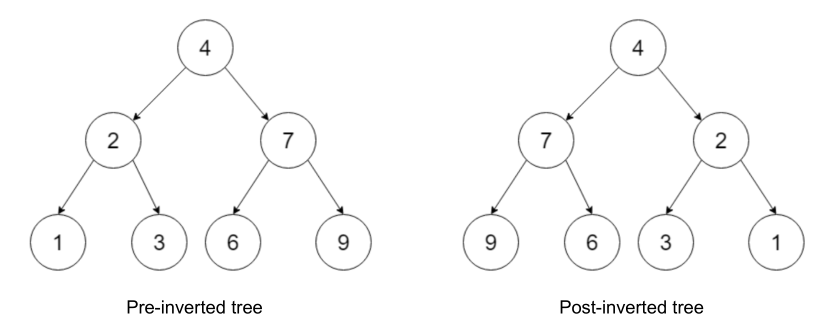
\includegraphics[width=0.5\paperwidth]{C:/Users/Admin/Desktop/Github/question_bank/static/img/9597-DHS-2021-P1-Q4-1}
\par\end{center}

Each node has these attributes: 
\begin{itemize}
\item \texttt{right} which is the pointer to right subtree 
\item \texttt{data} which is the value contained in each respective node
displayed above 
\item \texttt{left} which is the pointer to the left subtree
\end{itemize}
\begin{enumerate}
\item[(c)]  Write pseudocode for procedure \texttt{insert} which will add a
node to the post-inverted tree (which may be empty) in such a way
that if the new value of the node is \textbf{less} than the value
at the current node, the new node will be added to the \textbf{right}
subtree, or else it will be added to the left subtree. \texttt{insert}
takes in values \texttt{node\_data} and \texttt{root\_node} which
is the value to be added to the tree and the instance of the root
node of the tree respectively. \hfill{}{[}6{]}
\item[(d) ] A function \texttt{invertTree} takes in the root node of the above
pre-inverted tree, uses recursion to invert it into the post-inverted
tree, and returns the root node of the post-inverted tree. Write pseudocode
for the function and visualise it in a trace diagram. An incomplete
trace diagram is provided for you to begin with. Copy and complete
it. 
\noindent \begin{center}
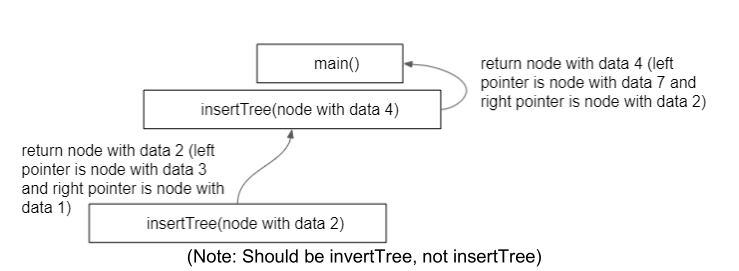
\includegraphics[width=0.5\paperwidth]{C:/Users/Admin/Desktop/Github/question_bank/static/img/9597-DHS-2021-P1-Q4-2}
\par\end{center}

(Note: Should be invertTree, not insertTree) \hfill{}{[}6{]}
\end{enumerate}

 \newpage 

\item \textbf{{[}DHS/PRELIM/9569/2021/P1/Q5{]} }

Consider the following data which shows a single Civics Group record
used in COVID19 vaccination tracking. 
\noindent \begin{center}
\includegraphics[width=0.5\paperwidth]{C:/Users/Admin/Desktop/Github/question_bank/static/img/9597-DHS-2021-P1-Q5}
\par\end{center}
\begin{enumerate}
\item Derive a set of tables to show the above data in first, second and
third normal form. \hfill{}{[}6{]}
\item Draw an ER diagram for a normalised database design. \hfill{} {[}2{]}
\item Using examples in the above context, explain the significance of the
following terms:
\begin{enumerate}
\item primary key \hfill{}{[}2{]}
\item foreign key \hfill{}{[}2{]}
\end{enumerate}
\item With reference to the above context, describe or suggest a scenario
where a NoSQL database would be more appropriate. \hfill{} {[}1{]}
\end{enumerate}

 \newpage 

\item \textbf{{[}DHS/PRELIM/9569/2021/P1/Q6{]} }

Long-distance optical fibre lines and submarine cables which are a
vital part of the global internet infrastructure are vulnerable to
solar superstorms which happen once in a century. The last solar superstrom
was in 1921. 
\begin{enumerate}
\item State and explain why websites would or would not be accessible by
web browsers if a solar superstorm shuts down all DNS servers. \hfill{}{[}2{]}
\item Explain packet switching and its importance in ensuring global internet
connectivity when some parts of the earth are hit by a solar superstorm.
\hfill{}{[}4{]}
\end{enumerate}
An international company based in many countries updates its network
structure to ensure Internet connectivity during solar superstorms. 

Employees can now access files on a shared virtual space which is
made up of 3 servers located in the United States, Europe, and Asia.
All servers hold identical information (any changes made on one server
would update the other servers immediately) so even if one server
is affected by the solar superstorm, employees still can access their
files on the other servers. 

Employees must be connected physically to the company\textquoteright s
intranet network at each country\textquoteright s office to access
the virtual space. 
\begin{enumerate}
\item[(c)] Draw a network diagram of the above configuration and label the LAN,
internet, router(s), WAN link(s), intranet, servers, and employee
laptops. \hfill{}{[}5{]}
\item[(d)] Why is version control vital when employees from different countries
work in teams? \hfill{}{[}1{]}
\end{enumerate}

 \newpage 

\item \textbf{{[}DHS/PRELIM/9569/2021/P1/Q7{]} }

A divide and conquer approach is used by merge sort to successively
divide a list into half, forming two sublists, until each sublist
is of length 1. The sublists are then sorted and merged into larger
sublists until they are recombined into a single sorted list. An algorithm
for merge sort to perform an ascending sort is given below. It will
be used to sort large or small data sizes. 

\noindent %
\noindent\begin{minipage}[t]{1\columnwidth}%
\texttt{01 PROCEDURE mergesort(mergelist : ARRAY) }

\texttt{02}

\texttt{03 \qquad{}IF LENGTH(mergelist) > 1 THEN }

\texttt{04 }

\texttt{05 \qquad{}\qquad{}mid \textleftarrow{} LENGTH(mergelist)
DIV 2 }

\texttt{06 }

\texttt{07 \qquad{}\qquad{}FOR index \textleftarrow{} 0 TO (mid
- 1) }

\texttt{08 \qquad{}\qquad{}\qquad{}lefthalf{[}index{]} \textleftarrow{}
mergelist{[}index{]} }

\texttt{09 \qquad{}\qquad{}NEXT index}

\texttt{10}

\texttt{11 \qquad{}\qquad{}right\_len \textleftarrow{} LENGTH(mergelist)
- mid}

\texttt{12}

\texttt{13 \qquad{}\qquad{}FOR index \textleftarrow{} 0 TO (right\_len
- 1) }

\texttt{14 \qquad{}\qquad{}\qquad{}righthalf{[}index{]} \textleftarrow{}
mergelist{[}right\_len + index{]} }

\texttt{15 \qquad{}\qquad{}NEXT index }

\texttt{16}

\texttt{17 \qquad{}\qquad{}mergesort(lefthalf) }

\texttt{18 \qquad{}\qquad{}mergesort(righthalf) }

\texttt{19}

\texttt{20 \qquad{}\qquad{}i \textleftarrow{} 0 }

\texttt{21 \qquad{}\qquad{}j \textleftarrow{} 0 }

\texttt{22 \qquad{}\qquad{}k \textleftarrow{} 0 }

\texttt{23 \qquad{}\qquad{}WHILE i < LENGTH(lefthalf) AND j < LENGTH(righthalf) }

\texttt{24 \qquad{}\qquad{}\qquad{}IF lefthalf{[}i{]} > righthalf{[}j{]}
THEN }

\texttt{25 \qquad{}\qquad{}\qquad{}\qquad{}mergelist{[}k{]} \textleftarrow{}
lefthalf{[}i{]}}

\texttt{26 \qquad{}\qquad{}\qquad{}\qquad{}i \textleftarrow{}
i + 1 }

\texttt{27 \qquad{}\qquad{}\qquad{}ELSE }

\texttt{28 \qquad{}\qquad{}\qquad{}\qquad{}mergelist{[}k{]} \textleftarrow{}
righthalf{[}j{]} }

\texttt{29 \qquad{}\qquad{}\qquad{}\qquad{}j \textleftarrow{}
j + 1 }

\texttt{30 \qquad{}\qquad{}\qquad{}ENDIF }

\texttt{31 \qquad{}\qquad{}\qquad{}k \textleftarrow{} k + 1}

\texttt{32 \qquad{}\qquad{}ENDWHILE }

\texttt{33}

\texttt{34 \qquad{}\qquad{}WHILE i < LENGTH(lefthalf) }

\texttt{35 \qquad{}\qquad{}\qquad{}mergelist{[}k{]} \textleftarrow{}
lefthalf{[}i{]} }

\texttt{36 \qquad{}\qquad{}\qquad{}i \textleftarrow{} i + 1 }

\texttt{37 \qquad{}\qquad{}\qquad{}k \textleftarrow{} k + 1 }

\texttt{38 \qquad{}\qquad{}ENDWHILE }

\texttt{39}

\texttt{40 \qquad{}\qquad{}WHILE j < LENGTH(righthalf) }

\texttt{41 \qquad{}\qquad{}\qquad{}mergelist(k{]} \textleftarrow{}
righthalf{[}j{]} }

\texttt{42 \qquad{}\qquad{}\qquad{}j \textleftarrow{} j + 1 }

\texttt{43 \qquad{}\qquad{}\qquad{}k \textleftarrow{} k + 1 }

\texttt{44 \qquad{}\qquad{}ENDWHILE }

\texttt{45 \qquad{}ENDIF }

\texttt{46 ENDPROCEDURE }%
\end{minipage}
\begin{enumerate}
\item The following array of numbers is to be sorted using \texttt{mergesort}: 
\noindent \begin{center}
\texttt{mergelist = {[}2, 4, 2, 8, 2, 8, 9, 1, 3{]}} 
\par\end{center}

What are the first two lists to be merged? \hfill{}{[}1{]}
\item Explain what a logic error is, give the line number for the logic
error in the above code, and rewrite the line correctly. \hfill{}
{[}2{]}
\end{enumerate}
The procedure\texttt{ sorting\_proc} uses an optimised bubble sort
to sort an array\texttt{ input\_array} in an ascending order. It is
used within \texttt{modified\_mergesort} which is a modified version
of \texttt{mergesort}. 

\noindent %
\noindent\begin{minipage}[t]{1\columnwidth}%
\texttt{01 PROCEDURE sorting\_proc(input\_array : ARRAY) }

\texttt{02}

\texttt{03 \qquad{}length \textleftarrow{} LENGTH(input\_array) }

\texttt{04}

\texttt{05 \qquad{}REPEAT }

\texttt{06 \qquad{}\qquad{}swapped \textleftarrow{} FALSE }

\texttt{07}

\texttt{08 \qquad{}\qquad{}FOR curr\_elem\_index \textleftarrow{}
1 to length \textendash{} 1 }

\texttt{09}

\texttt{10 \qquad{}\qquad{}\qquad{}IF input\_array {[}curr\_elem\_index
- 1{]} > input\_array {[}curr\_elem\_index{]} THEN }

\texttt{11 \qquad{}\qquad{}\qquad{}\qquad{}SWAP (input\_array
{[}curr\_elem\_index - 1{]}, input\_array {[}curr\_elem\_index{]}) }

\texttt{12 \qquad{}\qquad{}\qquad{}\qquad{}swapped \textleftarrow{}
TRUE }

\texttt{13 \qquad{}\qquad{}\qquad{}ENDIF}

\texttt{14 }

\texttt{15 \qquad{}\qquad{}ENDFOR}

\texttt{16}

\texttt{17 \qquad{}\qquad{}length \textleftarrow{} length \textendash{}
1 }

\texttt{18 }

\texttt{19 \qquad{}UNTIL NOT swapped }

\texttt{20}

\texttt{21 ENDPROCEDURE }%
\end{minipage}

\noindent %
\noindent\begin{minipage}[t]{1\columnwidth}%
\texttt{01 PROCEDURE modified\_mergesort(mergelist : ARRAY) }

\texttt{02 }

\texttt{03 \qquad{}IF LENGTH(mergelist) > 1 THEN }

\texttt{04 }

\texttt{05 \qquad{}\qquad{}IF LENGTH(mergelist) < 5 THEN }

\texttt{06 \qquad{}\qquad{}\qquad{}sorting\_proc(mergelist) }

\texttt{07 \qquad{}\qquad{}\qquad{}RETURN}

\texttt{08 }

\texttt{09 \qquad{}\qquad{}ELSE}

\texttt{10}

\texttt{11 \qquad{}\qquad{}\qquad{}mid \textleftarrow{} LENGTH(mergelist)
DIV 2 }

\texttt{12 }

\texttt{13 \qquad{}\qquad{}\qquad{}FOR index \textleftarrow{} 0
TO (mid - 1) }

\texttt{14 \qquad{}\qquad{}\qquad{}\qquad{}lefthalf{[}index{]}
\textleftarrow{} mergelist{[}index{]} }

\texttt{15 \qquad{}\qquad{}\qquad{}NEXT index}

\texttt{16}

\texttt{17 \qquad{}\qquad{}\qquad{}right\_len \textleftarrow{}
LENGTH(mergelist) - mid }

\texttt{18}

\texttt{19 \qquad{}\qquad{}\qquad{}FOR index \textleftarrow{} 0
TO (right\_len - 1) }

\texttt{20 \qquad{}\qquad{}\qquad{}\qquad{}righthalf{[}index{]}
\textleftarrow{} mergelist{[}right\_len + index{]} }

\texttt{21 \qquad{}\qquad{}\qquad{}NEXT index }

\texttt{22}

\texttt{23 \qquad{}\qquad{}\qquad{}mergesort(lefthalf) }

\texttt{24 \qquad{}\qquad{}\qquad{}mergesort(righthalf) }

\texttt{25}

\texttt{26 \qquad{}\qquad{}\qquad{}i \textleftarrow{} 0 }

\texttt{27 \qquad{}\qquad{}\qquad{}j \textleftarrow{} 0 }

\texttt{28 \qquad{}\qquad{}\qquad{}k \textleftarrow{} 0 }

\texttt{29 \qquad{}\qquad{}\qquad{}WHILE i < LENGTH(lefthalf) AND
j < LENGTH(righthalf) }

\texttt{30 \qquad{}\qquad{}\qquad{}\qquad{}IF lefthalf{[}i{]}
> righthalf{[}j{]} THEN }

\texttt{31 \qquad{}\qquad{}\qquad{}\qquad{}\qquad{}mergelist{[}k{]}
\textleftarrow{} lefthalf{[}i{]} }

\texttt{32 \qquad{}\qquad{}\qquad{}\qquad{}\qquad{}i \textleftarrow{}
i + 1 }

\texttt{33 \qquad{}\qquad{}\qquad{}\qquad{}ELSE }

\texttt{34 \qquad{}\qquad{}\qquad{}\qquad{}\qquad{}mergelist{[}k{]}
\textleftarrow{} righthalf{[}j{]}}

\texttt{35 \qquad{}\qquad{}\qquad{}\qquad{}\qquad{}j \textleftarrow{}
j + 1 }

\texttt{36 \qquad{}\qquad{}\qquad{}\qquad{}ENDIF }

\texttt{37 \qquad{}\qquad{}\qquad{}\qquad{}k \textleftarrow{}
k + 1 }

\texttt{38 \qquad{}\qquad{}\qquad{}ENDWHILE }

\texttt{39 }

\texttt{40 \qquad{}\qquad{}\qquad{}WHILE i < LENGTH(lefthalf) }

\texttt{41 \qquad{}\qquad{}\qquad{}\qquad{}mergelist{[}k{]} \textleftarrow{}
lefthalf{[}i{]} }

\texttt{42 \qquad{}\qquad{}\qquad{}\qquad{}i \textleftarrow{}
i + 1 }

\texttt{43 \qquad{}\qquad{}\qquad{}\qquad{}k \textleftarrow{}
k + 1}

\texttt{44 \qquad{}\qquad{}\qquad{}ENDWHILE}

\texttt{45 }

\texttt{46 \qquad{}\qquad{}\qquad{}WHILE j < LENGTH(righthalf)}

\texttt{47 \qquad{}\qquad{}\qquad{}\qquad{}mergelist{[}k{]} \textleftarrow{}
righthalf{[}j{]} }

\texttt{48 \qquad{}\qquad{}\qquad{}\qquad{}j \textleftarrow{}
j + 1 }

\texttt{49 \qquad{}\qquad{}\qquad{}\qquad{}k \textleftarrow{}
k + 1 }

\texttt{50 \qquad{}\qquad{}\qquad{}ENDWHILE }

\texttt{51 \qquad{}\qquad{}ENDIF }

\texttt{52 \qquad{}ENDIF }

\texttt{53 ENDPROCEDURE}%
\end{minipage}
\begin{enumerate}
\item[(c)]  Would the above modification of mergesort improve the algorithm\textquoteright s
overall efficiency? Support your answer with a description on how
and explanation on why its efficiency is affected. \hfill{} {[}4{]}
\end{enumerate}
The procedure \texttt{insertionSort} is an algorithm which uses insertion
sort. 

\noindent %
\noindent\begin{minipage}[t]{1\columnwidth}%
\texttt{01 PROCEDURE insertionSort(input\_array: ARRAY) }

\texttt{02 }

\texttt{03 \qquad{}current\_elem\_index \textleftarrow{} 0 }

\texttt{04 }

\texttt{05 \qquad{}REPEAT }

\texttt{06 \qquad{}\qquad{}current\_elem\_index \textleftarrow{}
current\_elem\_index + 1 }

\texttt{07 \qquad{}\qquad{}compared\_item\_index \textleftarrow{}
-1 }

\texttt{08 \qquad{}\qquad{}swapped \textleftarrow{} FALSE }

\texttt{09 }

\texttt{10 \qquad{}\qquad{}REPEAT }

\texttt{11 \qquad{}\qquad{}\qquad{}compared\_item\_index \textleftarrow{}
compared\_item\_index + 1 }

\texttt{12 }

\texttt{13 \qquad{}\qquad{}\qquad{}IF input\_array{[}current\_elem\_index{]}
< input\_array{[}compared\_item\_index{]} THEN }

\texttt{14 }

\texttt{15 \qquad{}\qquad{}\qquad{}\qquad{}temp \textleftarrow{}
input\_array{[}current\_elem\_index{]}}

\texttt{16 }

\texttt{17 \qquad{}\qquad{}\qquad{}\qquad{}the value of each element
of input\_array from compared\_item\_index to (current\_elem\_index
\textendash{} 1) is sequentially assigned to each element of input\_array
from (compared\_item\_index + 1) to current\_elem\_index}

\texttt{18 }

\texttt{19 \qquad{}\qquad{}\qquad{}\qquad{}input\_array{[}compared\_item\_index{]}
\textleftarrow{} temp }

\texttt{20 }

\texttt{21 \qquad{}\qquad{}\qquad{}\qquad{}swapped \textleftarrow{}
TRUE }

\texttt{22 \qquad{}\qquad{}\qquad{}ENDIF }

\texttt{23 }

\texttt{24 \qquad{}\qquad{}UNTIL swapped \textleftarrow{} TRUE }

\texttt{25 }

\texttt{26 \qquad{}UNTIL current\_elem\_index = LENGTH(input\_array)
- 1 }

\texttt{27 }

\texttt{28 ENDPROCEDURE }%
\end{minipage}
\begin{enumerate}
\item[(d)]  Modify \texttt{insertionSort} and \texttt{sorting\_proc} to count
and store the number of comparisons made in a variable named \texttt{comparisons}.
Instead of copying all the pseudocode statements, state the line number(s)
you want to modify or insert any pseudocode at, followed by the pseudocode
statement(s) to be added/modified. \hfill{}{[}3{]}
\item[(e)]  Trace the modified algorithms \texttt{insertionSort} and \texttt{sorting\_proc}
for the array \texttt{{[}5, 2, 3, 4{]}} showing the value of all variables
for each step by completing the following tables. 

Trace table for \texttt{insertionSort}: 

\texttt{}%
\begin{tabular}{|c|c|c|c|c|}
\hline 
\texttt{current\_elem \_index } & \texttt{compared\_item\_index } & \texttt{comparisons} & \texttt{input\_array} & \texttt{swapped}\tabularnewline
\hline 
\texttt{1} & \texttt{0} & \texttt{1} & \texttt{{[}2,5,3,4{]}} & \texttt{TRUE}\tabularnewline
\hline 
\texttt{2} & \texttt{0} & \texttt{2} & \texttt{{[}2,5,3,4{]}} & \texttt{FALSE}\tabularnewline
\hline 
... & ... & ... & ... & \tabularnewline
\hline 
\end{tabular}

Trace table for \texttt{sorting\_proc}: 

\texttt{}%
\begin{tabular}{|c|c|c|c|c|}
\hline 
\texttt{current\_elem \_index} & \texttt{compared\_item\_index} & \texttt{input\_array} & \texttt{arr\_length} & \texttt{swapped}\tabularnewline
\hline 
\texttt{1} & \texttt{1} & \texttt{{[}2,5,3,4{]}} & \texttt{4} & \texttt{TRUE}\tabularnewline
\hline 
\texttt{2} & 2 & \texttt{{[}2,5,3,4{]}} & \texttt{4} & \texttt{FALSE}\tabularnewline
\hline 
... & ... & \texttt{...} & ... & \texttt{...}\tabularnewline
\hline 
\end{tabular} 

\hfill{}{[}7{]}
\item[(f)]  In the context of \texttt{mergesort}, suggest scenario(s) where
using the current optimised bubble sort algorithm for \texttt{sorting\_proc}
would be better than using the \texttt{insertionSort} algorithm above.
Support your answer by designing 3 test cases (normal and boundary)
and comparing the number of \texttt{comparisons} made by each algorithm
for each test case. Display your output. \hfill{} {[}7{]}
\end{enumerate}

 \newpage 

\item \textbf{{[}DHS/PRELIM/9569/2021/P2/Q1{]} }

\textbf{Task 1}

For this task, submit all code as \texttt{T1\_<index number>\_<name>.py}. 

The Taliban\textquoteright s takeover of Afghanistan had seen the
United States (US) evacuating people. The Republic of Singapore Air
Force offers its A330 Multi-Role Tanker Transport plane (A330 MRTT)
to help the US airlift groups of evacuees from Afghanistan. 

\subsubsection*{Task 1.1 }

To prevent Taliban interference, messages sent between evacuees and
the A330 MRTT are encrypted. 

The encryption converts each character of the message into its ASCII
number representation, adds the ASCII number representation of a character
of a secret key which is in the same position, and then converts it
back into ASCII text. 

Secret keys are generated from passwords known only by the sender
and receiver. Passwords that are shorter in length than the message
are lengthened to match by repeating the password until the same length
as the message is achieved. 

For example, given that the inputs are 

\texttt{password : \textquotedbl cat\textquotedbl{} }

\texttt{message ~: \textquotedbl hello\textquotedbl} 

Step 1 - Extend password by repeating until matches length of message 

\texttt{\textquotedbl cat\textquotedbl{} -> \textquotedbl catca\textquotedbl{} }

Step 2 - Convert each character of password and message into ASCII
number representation 

\texttt{\textquotedbl hello\textquotedbl{} -> 104, 101, 108, 108,
111 }

\texttt{\textquotedbl catca\textquotedbl{} -> 99, 97, 116, 99, 97 }

Step 3 - Add the ASCII number representation of same positions together 

\texttt{104+99, 101+97, 108+116, 108+99, 111+97 -> 203, 198, 224,
207, 208 }

Step 4 - Convert each number to its ASCII character 

\texttt{203, 198, 224, 207, 208 -> \textquotedbl �����\textquotedbl{} }

Therefore, the results are 

\texttt{Secret key : \textquotedbl catca\textquotedbl{} }

\texttt{Encrypted message : \textquotedbl �����\textquotedbl{} }

Write a function \texttt{generateKey(password, message)} that takes
in two argument strings \texttt{message} and \texttt{password} and
returns the secret key. 

Test your function using \texttt{generateKey(\textquotedbl cat\textquotedbl ,
\textquotedbl hello\textquotedbl )} and show your output. \hfill{}{[}4{]}

\subsubsection*{Task 1.2 }

Write functions \texttt{encrypt(password, message)} and \texttt{decrypt(password,
message)} that takes in \texttt{password} and message strings and
returns the encrypted or decrypted \texttt{message}. It should use
the above function \texttt{generateKey(password, message)} to obtain
the secret key before performing the encryption. 

Test your function with \texttt{decrypt(\textquotedbl cat\textquotedbl ,
encrypt(\textquotedbl cat\textquotedbl ,\textquotedbl hello\textquotedbl ))}.
Show your output. \hfill{}{[}6{]}

\subsubsection*{Task 1.3 }

Since the A330 MRTT plane can only take a maximum of 266 passengers
at once, implement a \texttt{Queue} to manage incoming pickup requests
and dropoffs. Write a class Queue with the following methods: 
\begin{itemize}
\item \texttt{enqueue(string)} which takes in a string and adds it to the
queue or returns \texttt{\textquotedbl Queue is full!\textquotedbl}
if queue is full 
\item \texttt{dequeue} which removes the next item for the queue or returns
\texttt{\textquotedbl Queue is empty!\textquotedbl} if the queue
is empty 
\item \texttt{display} which returns a string of queue items in sequence
from head to tail or returns \texttt{\textquotedbl Queue is empty!\textquotedbl}
if the queue is empty
\item \texttt{current\_size} which returns an integer of the number of items
in the queue. \hfill{}{[}8{]}
\end{itemize}

\subsubsection*{Task 1.4 }

Using socket programming, write the client program for the evacuee
teams (client) in Afghanistan and the A330 MRTT plane (server) to
communicate. The program should 
\begin{itemize}
\item use the above queue data structure to manage the requests 
\item request the user to set a password for encryption at the start of
the program 
\item present the user with incoming pickup requests and pickup details
(Team name and group size) as well as queue details (size of current
queue) 
\item allow the user(server) to accept/reject pickup requests 
\item encrypt all information sent and received using \texttt{encrypt(password,
message)} and \texttt{decrypt(password, message)} functions. 
\end{itemize}
You are provided with the client program in \texttt{client.py}. Write
and submit the server program as \texttt{T1\_<index number>\_<name>.py}. 

Study the following sample program output to determine your code design,
output format and socket protocol. User inputs are underlined. 

\noindent %
\noindent\fbox{\begin{minipage}[t]{1\columnwidth - 2\fboxsep - 2\fboxrule}%
\textbf{Sample server program:}

\texttt{Please set a password: Answer: }\texttt{\uline{WDIB4}}\texttt{ }

\texttt{Next action? }

\texttt{Menu: }

\texttt{1) Wait for connection from client for next pickup request }

\texttt{2) Dequeue }

\texttt{Type an option:}\texttt{\uline{2}}\texttt{ \bigskip{}
}

\texttt{Queue is empty! \bigskip{}
}

\texttt{Next action? }

\texttt{Menu:}

\texttt{1) Wait for connection from client for next pickup request }

\texttt{2) Dequeue }

\texttt{Type an option:}\texttt{\uline{1}}\texttt{ }

\texttt{\bigskip{}
Awaiting connection from pickup client... }

\texttt{\bigskip{}
Connection established! }

\texttt{Receiving data from client\dots{} }

\texttt{Checking client's secret key\dots{} }

\texttt{Client's secret key is correct! }

\texttt{\bigskip{}
Client's Team name: Team1 }

\texttt{Group size: 143}

\texttt{No. of passengers in queue: 0 }

\texttt{You have capacity for them. }

\texttt{\bigskip{}
Confirm pickup? Y/N? }

\texttt{Answer:}\texttt{\uline{Y}}\texttt{ \bigskip{}
}

\texttt{Added to queue. }

\texttt{Items in queue now are: Team1, Team1, Team1, Team1, Team1,
Team1, Team1, Team1, Team1, Team1, Team1, Team1, Team1, Team1, Team1,
Team1, Team1, Team1, Team1, Team1, Team1, Team1, Team1, Team1, Team1,
Team1, Team1, Team1, Team1, Team1, Team1, Team1, Team1, Team1, Team1,
Team1, Team1, Team1, Team1, Team1, Team1, Team1, Team1, Team1, Team1,
Team1, Team1, Team1, Team1, Team1, Team1, Team1, Team1, Team1, Team1,
Team1, Team1, Team1, Team1, Team1, Team1, Team1, Team1, Team1, Team1,
Team1, Team1, Team1, Team1, Team1, Team1, Team1, Team1, Team1, Team1,
Team1, Team1, Team1, Team1, Team1, Team1, Team1, Team1, Team1, Team1,
Team1, Team1, Team1, Team1, Team1, Team1, Team1, Team1, Team1, Team1,
Team1, Team1, Team1, Team1, Team1, Team1, Team1, Team1, Team1, Team1,
Team1, Team1, Team1, Team1, Team1, Team1, Team1, Team1, Team1, Team1,
Team1, Team1, Team1, Team1, Team1, Team1, Team1, Team1, Team1, Team1,
Team1, Team1, Team1, Team1, Team1, Team1, Team1, Team1, Team1, Team1,
Team1, Team1, Team1, Team1, Team1, Team1, Team1, Team1, }

\texttt{Connection disconnected. }

\texttt{\bigskip{}
Next action? Menu: }

\texttt{1) Wait for connection from client for next pickup request }

\texttt{2) Dequeue }

\texttt{Type an option:}\texttt{\uline{1}}\texttt{ }

\texttt{\bigskip{}
Awaiting connection from pickup client... }

\texttt{\bigskip{}
Connection established! }

\texttt{Receiving data from client\dots{} }

\texttt{Checking client's secret key\dots{} }

\texttt{Client's secret key is correct! }

\texttt{\bigskip{}
Client's Team name: Team2 }

\texttt{Group size: 151 }

\texttt{No. of passengers in queue: 143 }

\texttt{You do NOT have capacity for them. }

\texttt{Connection disconnected. \bigskip{}
Next action? }

\texttt{Menu: }

\texttt{1) Wait for connection from client for next pickup request }

\texttt{2) Dequeue }

\texttt{Type an option:}\texttt{\uline{1}}\texttt{ }

\texttt{\bigskip{}
}

\texttt{Awaiting connection from pickup client... }

\texttt{\bigskip{}
Connection established! }

\texttt{Receiving data from client\dots{} }

\texttt{Checking client's secret key\dots{} }

\texttt{Client's secret key is correct!\bigskip{}
}

\texttt{Client's Team name: Team3 }

\texttt{Group size: 19 }

\texttt{No. of passengers in queue: 143}

\texttt{You have capacity for them. \bigskip{}
}

\texttt{Confirm pickup? Y/N? }

\texttt{Answer:}\texttt{\uline{N}}\texttt{ }

\texttt{\bigskip{}
Connection disconnected. \bigskip{}
Next action? }

\texttt{Menu: }

\texttt{1) Wait for connection from client for next pickup request }

\texttt{2) Dequeue }

\texttt{Type an option:}\texttt{\uline{1}}\texttt{ }

\texttt{\bigskip{}
Awaiting connection from pickup client... }

\texttt{\bigskip{}
Connection established! }

\texttt{Receiving data from client\dots{} }

\texttt{Checking client's secret key\dots{} }

\texttt{Client's secret key is correct!}

\texttt{\bigskip{}
Client's Team name: Team4 }

\texttt{Group size: 15 }

\texttt{No. of passengers in queue: 143 }

\texttt{You have capacity for them. }

\texttt{\bigskip{}
Confirm pickup? Y/N? }

\texttt{Answer:}\texttt{\uline{Y}}\texttt{ }

\texttt{\bigskip{}
Added to queue. Items in queue now are: }

\texttt{Team1, Team1, Team1, Team1, Team1, Team1, Team1, Team1, Team1,
Team1, Team1, Team1, Team1, Team1, Team1, Team1, Team1, Team1, Team1,
Team1, Team1, Team1, Team1, Team1, Team1, Team1, Team1, Team1, Team1,
Team1, Team1, Team1, Team1, Team1, Team1, Team1, Team1, Team1, Team1,
Team1, Team1, Team1, Team1, Team1, Team1, Team1, Team1, Team1, Team1,
Team1, Team1, Team1, Team1, Team1, Team1, Team1, Team1, Team1, Team1,
Team1, Team1, Team1, Team1, Team1, Team1, Team1, Team1, Team1, Team1,
Team1, Team1, Team1, Team1, Team1, Team1, Team1, Team1, Team1, Team1,
Team1, Team1, Team1, Team1, Team1, Team1, Team1, Team1, Team1, Team1,
Team1, Team1, Team1, Team1, Team1, Team1, Team1, Team1, Team1, Team1,
Team1, Team1, Team1, Team1, Team1, Team1, Team1, Team1, Team1, Team1,
Team1, Team1, Team1, Team1, Team1, Team1, Team1, Team1, Team1, Team1,
Team1, Team1, Team1, Team1, Team1, Team1, Team1, Team1, Team1, Team1,
Team1, Team1, Team1, Team1, Team1, Team1, Team1, Team1, Team1, Team1,
Team1, Team1, Team1, Team1, Team4, Team4, Team4, Team4, Team4, Team4,
Team4, Team4, Team4, Team4, Team4, Team4, Team4, Team4, Team4, }

\texttt{Connection disconnected. }

\texttt{\bigskip{}
Next action? }

\texttt{Menu: }

\texttt{1) Wait for connection from the next pickup location client }

\texttt{2) Dequeue }

\texttt{Type an option:}\texttt{\uline{2}}\texttt{ }

\texttt{\bigskip{}
How many to dequeue? 143}

\texttt{\bigskip{}
Items in queue now are: }

\texttt{Team4, Team4, Team4, Team4, Team4, Team4, Team4, Team4, Team4,
Team4, Team4, Team4, Team4, Team4, Team4, }

\texttt{Connection disconnected. }

\texttt{\bigskip{}
Next action? }

\texttt{Menu: }

\texttt{1) Wait for connection from client for next pickup request }

\texttt{2) Dequeue}

\texttt{Type an option:}\texttt{\uline{1}}\texttt{ }

\texttt{\bigskip{}
Awaiting connection from pickup client... }

\texttt{\bigskip{}
Connection established! }

\texttt{Receiving data from client\dots{} }

\texttt{Wrong secret key. }

\texttt{Connection disconnected. }

\texttt{\bigskip{}
Next action? }

\texttt{Menu: }

\texttt{1) Wait for connection from client for next pickup request }

\texttt{2) Dequeue }

\texttt{Type an option:}%
\end{minipage}}

\noindent %
\noindent\fbox{\begin{minipage}[t]{1\columnwidth - 2\fboxsep - 2\fboxrule}%
\texttt{Sample client programs (in sequence): }

\texttt{\textbf{\emph{CLIENT 1 }}}

\texttt{Please set a password. }

\texttt{Answer: }\texttt{\uline{WDIB4 }}

\texttt{\bigskip{}
}

\texttt{What is your Team Name? }

\texttt{Answer: }\texttt{\uline{Team1}}\texttt{ }

\texttt{\bigskip{}
}

\texttt{Group size?}

\texttt{Answer: }\texttt{\uline{143}}\texttt{ }

\texttt{\bigskip{}
}

\texttt{Establishing connection... }

\texttt{Connection established! }

\texttt{Data sent! }

\texttt{\bigskip{}
}

\texttt{Waiting for the server to confirm your request\dots{} }

\texttt{\bigskip{}
}

\texttt{Pickup confirmed! Please wait for pickup. }

\texttt{\bigskip{}
}

\texttt{Connection disconnected. }

\texttt{\bigskip{}
}

\texttt{\textbf{\emph{CLIENT 2}}}\texttt{\emph{ }}

\texttt{Please set a password. }

\texttt{Answer: }\texttt{\uline{WDIB4}}\texttt{ solver(\textquotedbl ((1{*}7)+6)\textquotedbl )\bigskip{}
}

\texttt{What is your Team Name? }

\texttt{Answer: }\texttt{\uline{Team2}}\texttt{ \bigskip{}
}

\texttt{Group size? }

\texttt{Answer: }\texttt{\uline{151}}\texttt{ \bigskip{}
}

\texttt{Establishing connection... }

\texttt{Connection established! }

\texttt{Data sent! \bigskip{}
}

\texttt{Waiting for the server to confirm your request\dots{} \bigskip{}
}

\texttt{Pickup rejected! }

\texttt{Wrong password or request rejected. }

\texttt{Please try again. Connection disconnected. \bigskip{}
}

\texttt{\textbf{\emph{CLIENT 3}}}\texttt{ }

\texttt{Please set a password. }

\texttt{Answer: }\texttt{\uline{WDIB4}}\texttt{ \bigskip{}
}

\texttt{What is your Team Name? }

\texttt{Answer: }\texttt{\uline{Team3}}\texttt{ \bigskip{}
}

\texttt{Group size? }

\texttt{Answer: }\texttt{\uline{19}}\texttt{ \bigskip{}
}

\texttt{Establishing connection... }

\texttt{Connection established! }

\texttt{Data sent! \bigskip{}
}

\texttt{Waiting for the server to confirm your request\dots{} \bigskip{}
}

\texttt{Pickup rejected! }

\texttt{Wrong password or request rejected. }

\texttt{Please try again. \bigskip{}
}

\texttt{Connection disconnected. \bigskip{}
}

\texttt{\textbf{\emph{CLIENT 4 }}}

\texttt{Please set a password. }

\texttt{Answer: }\texttt{\uline{WDIB4}}\texttt{ \bigskip{}
}

\texttt{What is your Team Name? }

\texttt{Answer: }\texttt{\uline{Team4}}\texttt{ \bigskip{}
}

\texttt{Group size? }

\texttt{Answer: }\texttt{\uline{15}}\texttt{ \bigskip{}
}

\texttt{Establishing connection... }

\texttt{Connection established! }

\texttt{Data sent! \bigskip{}
}

\texttt{Waiting for the server to confirm your request\dots{} \bigskip{}
}

\texttt{Pickup confirmed! Please wait for pickup to arrive. \bigskip{}
}

\texttt{Connection disconnected. \bigskip{}
}

\texttt{\textbf{\emph{CLIENT 4 }}}

\texttt{Please set a password. }

\texttt{Answer: }\texttt{\uline{FEWF}}\texttt{ }

\texttt{What is your Team Name? }

\texttt{Answer: }\texttt{\uline{Team5}}\texttt{ }

\texttt{Group size? }

\texttt{Answer: }\texttt{\uline{10}}\texttt{ \bigskip{}
}

\texttt{Establishing connection... }

\texttt{Connection established! }

\texttt{Data sent! \bigskip{}
}

\texttt{Waiting for the server to confirm your request\dots{} \bigskip{}
}

\texttt{Pickup cancelled. }

\texttt{Wrong password or request rejected. }

\texttt{Please try again. \bigskip{}
}

\texttt{Connection disconnected.}%
\end{minipage}}

\hfill{}{[}15{]}

 \newpage 

\item \textbf{{[}DHS/PRELIM/9569/2021/P2/Q2{]} }

\textbf{Task 2} 

Name your Jupyter Notebook and save all parts for this task as 

\texttt{TASK2\_<index\_number>\_<name>.ipynb }

You will be writing a Math game program for Form Teachers to play
with students in school. The game auto-generates math expressions
and tracks scoring. 

\subsubsection*{Task 2.1 }

Using a stack data structure, write a function \texttt{solver(expr)}
that takes in a string of a mathematical expression expr such as \texttt{\textquotedbl ((1{*}7)+6)\textquotedbl}
and returns \texttt{13}. You may assume that the entire expression
would never have spaces, and would always be enclosed in an opening
and closing parenthesis \textquotedbl ( )\textquotedbl . Do not
use the built-in function \texttt{eval()}. Test your function with
\texttt{solver(\textquotedbl ((1{*}7)+6)\textquotedbl )} and show
your output. \hfill{}{[}6{]}

\subsubsection*{Task 2.2 }

Write a function \texttt{generate\_expression} that takes in an integer
\texttt{operator\_count} and returns a string of a mathematical expression
which has the specified number of operators (i.e. \texttt{+ - {*}
/} ) in \texttt{operator\_count}. The function should use \textbf{recursion}
to form up the operators and operands. The operands, operators and
positions of operands and operators should be random. 

For example, \texttt{generate\_expression(5)} would output \textquotedbl\texttt{(4{*}(6-(2+((1{*}7)+6))))}\textquotedbl{}
and \texttt{generate\_expression(5}) would output \textquotedbl\texttt{((8+(6+((2{*}4)-3)))+6)}\textquotedbl . 

Test your function with \texttt{generate\_expression(5)} and show
your output. \hfill{}{[}7{]}

\subsubsection*{Task 2.3 }

Implement the following using object-oriented programming: 
\begin{itemize}
\item \texttt{Person}, a class, which 
\begin{itemize}
\item initialises with these attributes 
\begin{itemize}
\item \texttt{name: string }
\item \texttt{gender: string} where male is \textquotedbl\texttt{M}\textquotedbl{}
and female is \textquotedbl\texttt{F}\textquotedbl{} 
\item \texttt{score: integer }
\end{itemize}
\item has the following methods 
\begin{itemize}
\item \texttt{display\_info()} which displays the \texttt{Person}\textquoteright s
\texttt{name}, \texttt{gende}r and \texttt{score} 
\begin{itemize}
\item 1. eg \textquotedbl\texttt{Nelson(M)\textquoteright s score is 3.}\textquotedbl{} 
\end{itemize}
\item \texttt{attempts()} which
\begin{itemize}
\item 1. uses the function \texttt{generate\_expression} from Task 2.2 to
generate and display a random math expression of 2 operators 
\item 2. queries the user to give an answer rounded up to the nearest integer 
\item 3. displays \textquotedbl\texttt{Good job!}\textquotedbl{} if the
input is correct or \textquotedbl\texttt{Wrong answer. (Correct
answer: <answer>)}\textquotedbl{} where \texttt{<answer>} is the correct
answer. 
\item 4. increases the score of the student by \texttt{1} if the answer
is correct 
\item 5. displays the user\textquoteright s latest \texttt{sc}ore 
\end{itemize}
\end{itemize}
\end{itemize}
\item \texttt{Student}, a subclass of \texttt{Person}, which 
\begin{itemize}
\item also has the following attribute 
\begin{itemize}
\item \texttt{role: string} which is \textquotedbl\texttt{no role}\textquotedbl{}
by default unless the \texttt{Student} has a class committee role
such as \textquotedbl\texttt{chairperson}\textquotedbl{} 
\end{itemize}
\item also has the following methods 
\begin{itemize}
\item \texttt{student\_role()} which returns a string describing the \texttt{role}
of the \texttt{Student}
\end{itemize}
\end{itemize}
\item \texttt{FormTeacher}, a subclass of \texttt{Person}, which 
\begin{itemize}
\item also has the following methods
\begin{itemize}
\item \texttt{display\_info()} which uses polymorphism to display the\texttt{
FormTeacher}\textquoteright s information with salutation to the FormTeacher\textquoteright s
name 
\begin{itemize}
\item 1. eg: \textquotedbl\texttt{Ms. Norah's score is 0}.\textquotedbl{}
where \textquotedbl\texttt{Norah}\textquotedbl{} is her name, and
\textquotedbl\texttt{Ms}.\textquotedbl{} corresponds to her gender.
\hfill{} {[}14{]}
\end{itemize}
\end{itemize}
\end{itemize}
\end{itemize}

\subsubsection*{Task 2.4}

Write driver code to test the earlier class you created. Also, create
\texttt{groups} which is a list that uses a 2-dimensional array to
store and associate each instance created below with his/her civics
group. Use this 2-dimensional array to display the scores of all persons
in each civics group indicating the student chairperson\textquoteright s
name (if any). Test your code with the following steps in order: 
\begin{itemize}
\item Create an instance of \texttt{Student} with \texttt{name} \textquotedbl\texttt{Melvin}\textquotedbl{}
in civics group \texttt{5C35} 
\item Create an instance of \texttt{Student} with \texttt{name} \textquotedbl\texttt{Susan}\textquotedbl{}
in civics group \texttt{5C35} whose role is \textquotedbl\texttt{chairperson}\textquotedbl{} 
\item Create an instance information of \texttt{FormTeacher} with \texttt{name}
\textquotedbl\texttt{Norah}\textquotedbl{} in civics group \texttt{5C35} 
\item Create an instance of \texttt{Student} with name \textquotedbl\texttt{Ben}\textquotedbl{}
in civics group \texttt{6C35} 
\item Create an instance of \texttt{FormTeacher} with name \textquotedbl\texttt{Jimmy}\textquotedbl{}
in civics group \texttt{6C35} 
\item Display the information of Melvin 
\item Display the information of Susan 
\item Display the information of Norah 
\item Melvin attempts a math question 
\item Susan attempts a math question 
\item Jimmy attempts a math question 
\item Display the scores of all persons in each civics group with a header
for each class 
\end{itemize}
Here is a sample of an expected output: 

\noindent %
\noindent\begin{minipage}[t]{1\columnwidth}%
\texttt{Melvin(M)'s score is 0. }

\texttt{Susan(F)'s score is 0. }

\texttt{Ms. Norah's score is 0. \bigskip{}
}

\texttt{To Melvin : ((5/7)+8) ? }

\texttt{Answer:1 }

\texttt{Wrong answer. (Correct answer: 9 ) }

\texttt{Total score is still 0. \bigskip{}
}

\texttt{To Susan : (3{*}(5{*}6)) ? }

\texttt{Answer:90 }

\texttt{Good job! }

\texttt{New total score for Susan is 1 \bigskip{}
}

\texttt{To Jimmy : ((6-2)-6) ? }

\texttt{Answer:3 }

\texttt{Wrong answer. }

\texttt{(Correct answer: -2 ) }

\texttt{Total score is still 0. \bigskip{}
}

\texttt{5C35\textquoteright s scores:}

\texttt{Melvin(M)'s score is 0. }

\texttt{Susan(F)'s score is 1. (Chairperson) }

\texttt{Ms. Norah's score is 0.\bigskip{}
}

\texttt{6C35\textquoteright s scores:}

\texttt{Ben(M)'s score is 0. }

\texttt{Mr. Jimmy's score is 0. }%
\end{minipage}

Run your program and save your output. \hfill{}{[}7{]}

 \newpage 

\item \textbf{{[}DHS/PRELIM/9569/2021/P2/Q3{]} }

\textbf{Task 3} 

In 2021, Singapore's Health Science Authority (HSA) recalled 18 brands
of hand sanitisers due to high levels of acetaldehyde and/or methanol.
The HSA keeps information on current hand sanitisers and uses it to
monitor the types of chemical ingredients used to make the sanitisers. 

\subsubsection*{Task 3.1 }

Create an SQL file to show the SQL code to create database \texttt{sanitisers.db}
with the single table, \texttt{sanitisers}. 

The table will have the following fields: 
\begin{itemize}
\item \texttt{product\_name} which is the primary key 
\item \texttt{active\_ingredient} 
\item \texttt{alcohol-based} 
\end{itemize}
Save your SQL code as 

\texttt{TASK3\_<index\_number>\_<name>.sql} \hfill{}{[}3{]}

\subsubsection*{Task 3.2}

The text file, \texttt{sanitisers.txt}, contains data items for a
number of sanitisers. It contains a header line. Each data item is
separated by a comma, with each item data on a new line, as follows:
\begin{itemize}
\item product name 
\item active ingredient used to make the sanitiser product 
\item \textquotedbl Yes\textquotedbl{} or \textquotedbl No\textquotedbl{}
to indicate if the product is alcohol-based 
\end{itemize}
Write program code to read in the information from the text file,
\texttt{sanitisers.txt}, and insert all the information into the \texttt{sanitisers.db}
database. \hfill{}{[}3{]}

Run the program. 

Save your program as 

\texttt{TASK3\_<index\_number>\_<name>.py} 

\subsubsection*{Task 3.3}

The information is to be displayed in a web browser. 

Write a python program and the necessary files to create a web application
that enables the list of sanitisers to be displayed. 

For each record the web page should include the: 
\begin{itemize}
\item product name 
\item ingredients used to make the sanitiser product
\item \textquotedbl Yes\textquotedbl{} or \textquotedbl No\textquotedbl{}
to indicate if the product is alcohol-based 
\end{itemize}
Save your program as 

\texttt{TASK3\_<index\_number>\_<name>.py} 

with any additional files/subfolders as needed in a folder named 

\texttt{TASK3\_<index\_number>\_<name>} 

Run the web application and save the output of the program as 

\texttt{TASK3\_OUTPUT\_<index\_number>\_<name>.html}\hfill{} {[}6{]}

\subsubsection*{Task 3.4 }

HSA wants a form on the web page that allows users to enter in the
name of an active ingredient and, upon submission, will display all
the information of the products with the matching active ingredient. 

Update your application to include this form feature so that users
will be able to use the form after seeing the list of sanitisers displayed
as required in Task 3.3. 

Run the web application, test your program with the ingredient \textquotedbl\texttt{Triclosan}\textquotedbl{}
and save the output. \hfill{}{[}4{]}

Save, zip up and submit your program code and all related files for
Task 3 as 

\texttt{TASK3\_<index\_number>\_<name>.zip}

 \newpage 

\item \textbf{{[}DHS/PRELIM/9569/2021/P2/Q4{]} }

\textbf{Task 4}

Name your Jupyter Notebook and save all parts for this task as 

\texttt{TASK4\_<index\_number>\_<name>.ipynb }

\subsubsection*{Task 4.1 }

Write a program to help staff of an events company to insert data
into a NoSQL database products under the collection \texttt{balloons}. 

The data is provided for you in \texttt{balloons.json} as well as
in the table below where the first row are headers for the fields. 
\noindent \begin{center}
\begin{tabular}{|c|c|c|c|}
\hline 
\texttt{design } & \texttt{amount } & \texttt{helium} & \texttt{colours}\tabularnewline
\hline 
car  & 88  & no & red, yellow\tabularnewline
\hline 
cloud  & 14  &  & blue, green\tabularnewline
\hline 
flower  & 75  & yes & red, blue\tabularnewline
\hline 
bag  & 38  & no  & red, blue, black\tabularnewline
\hline 
\end{tabular}
\par\end{center}

Each colour in \texttt{colours} field should be an item in an array.
\hfill{}{[}6{]}

\subsubsection*{Task 4.2 }

Write code to print the \texttt{amount} of the product with the design
\textquotedbl\texttt{car}\textquotedbl .\hfill{} {[}2{]}

\subsubsection*{Task 4.3 }

Write code to update the field \texttt{helium} to have the value \textquotedbl\texttt{n}o\textquotedbl{}
for all documents which do not have a field or value for \texttt{helium}.
\hfill{}{[}3{]}

\subsubsection*{Task 4.4 }

Write code to display the \texttt{design}(s) which do not contain
helium and have colours that either contain \texttt{green} or do not
contain \texttt{black}. \hfill{}{[}3{]}

Run the program.

 \newpage 

\item \textbf{{[}HCI/PRELIM/9569/2021/P1/Q1{]} }

An E-Commerce company stores the following data of customers in the
system. 
\begin{itemize}
\item Name 
\item Contact 
\item Address 
\end{itemize}
It categories its customers into 2 types of loyalty programs. 
\begin{itemize}
\item Spend-based loyalty program 
\item Paid loyalty program 
\end{itemize}
Customers of Spend-based loyalty program earn one point for every
block of \$10 spent in a single order, whereas customers of Paid loyalty
program pay a monthly or annual fee. Customers of Paid loyalty program
will enjoy the benefits of having early access to sales events and
free delivery for purchases above \$30. 

For Spend-based loyalty program, the additional data stored include: 
\begin{itemize}
\item Points earned 
\end{itemize}
For Paid loyalty program, the additional data stored include: 
\begin{itemize}
\item Payment schedule (monthly or annually) and corresponding fee 
\item Next payment date, computed based on payment schedule and the date
of enrollment to the program 
\end{itemize}
Object-oriented programming will be used to model the customers. 
\begin{enumerate}
\item Draw a class diagram that shows the following for the requirement
described above.
\begin{itemize}
\item the superclass 
\item any subclasses 
\item inheritance 
\item properties 
\item appropriate methods \hfill{}{[}6{]}
\end{itemize}
\end{enumerate}
The company makes changes to the Paid loyalty program to allow the
customer in the program to earn ten points for every block of \$20
spent in a single order, in addition to the current benefits. The
points earned do not expire. For Spend- based loyalty program, all
points earned will expire on the anniversary of the date of enrolment
to the program. 
\begin{enumerate}
\item[(b)]  Suggest changes required to the class diagram to enable the changes.\hfill{}
{[}3{]}
\item[(c)]  Explain why inheritance is an important feature of object-oriented
programming.\hfill{} {[}1{]}
\end{enumerate}
To attract customers to enrol to its Paid loyalty program, the company
launches an invitation campaign to invite Spend-based loyalty program
customers who qualified the following conditions: 
\begin{itemize}
\item Customer who earned more than 2000 points in a year and has an average
of at least one order per month will be contacted by staff. 
\item Customer who has enrolled for at least a year and has an average of
at least one order per month will be sent an invitation email. 
\item Otherwise, no invitation will be sent. 
\end{itemize}
\begin{enumerate}
\item[(d)]  Create a decision table showing all the possible outcomes and results.
\hfill{}{[}4{]}
\item[(e)]  Simplify your decision table by removing redundancies.\hfill{}
{[}2{]}
\end{enumerate}

 \newpage 

\item \textbf{{[}HCI/PRELIM/9569/2021/P1/Q2{]}}

Merge Sort is a Divide and Conquer algorithm. It divides the unsorted
array \texttt{A{[}low..high{]}} into two halves, calls itself for
the two halves, until each half is of length 1. It then merges the
two sorted halves. An algorithm for Merge Sort is given below. 

\noindent %
\noindent\begin{minipage}[t]{1\columnwidth}%
\texttt{PROCEDURE MergeSort(A, low, high) }

\texttt{\qquad{}IF low < high }

\texttt{\qquad{}\qquad{}mid \textleftarrow{} (low + high) DIV 2 }

\texttt{\qquad{}\qquad{}MergeSort(A, low, mid) }

\texttt{\qquad{}\qquad{}MergeSort(A, mid+1, high) }

\texttt{\qquad{}\qquad{}Merge(A, low, mid, high) }

\texttt{\qquad{}ENDIF }

\texttt{ENDPROCEDURE }%
\end{minipage}
\begin{enumerate}
\item Write in \textbf{pseudocode}, an algorithm for the merge procedure,
\texttt{Merge(A, low, mid, high)} that is called by the \texttt{MergeSort}
algorithm. The merge procedure should merge the sorted subarrays in
\texttt{A{[}low..mid{]}} and \texttt{A{[}mid+1..high{]}} into a single
sorted subarray in \texttt{A{[}low..high{]}}. \hfill{}{[}6{]}
\item Give and justify the time complexity of Merge Sort. \hfill{}{[}2{]}
\end{enumerate}

 \newpage 

\item \textbf{{[}HCI/PRELIM/9569/2021/P1/Q3{]}}

An abstract Data Type (ADT) consists of both data type and associated
operations. 

A stack ADT has the following operations defined: 
\begin{itemize}
\item Create(S) -{}-{}- creates an empty stack S, 
\item Insert(S, Item) -{}-{}- inserts new value, Item, onto stack S, 
\item Retrieve(S) -{}-{}- removes and returns item from the stack S, 
\item EmptyStack(S) -{}-{}- returns true if stack S is empty. 
\end{itemize}
\begin{enumerate}
\item Devise an algorithm that converts a non-negative integer from decimal
to hexadecimal, by making use of the stack operations given above.
\hfill{}{[}4{]}
\item Three items, L1, L2 and L3, are to be inserted into a stack in its
original order, but the output would be in the order of L1, L3 and
L2. 

Write an algorithm, using the operations given above, that would use
a stack R to carry this out. \hfill{}{[}4{]}
\end{enumerate}

 \newpage 

\item \textbf{{[}HCI/PRELIM/9569/2021/P1/Q4{]}}

Some algorithms can be written using recursion.
\begin{enumerate}
\item State \textbf{two} features of recursion. \hfill{}{[}2{]}
\item Explain the use of a stack when the recursive procedure executes.
\hfill{}{[}3{]}
\item Write a recursive function using \textbf{pseudocode} that returns
the sum of the digits in an integer. For example, the sum of the digits
of the integer \texttt{12345} is \texttt{5+4+3+2+1=15}. \hfill{}{[}4{]}
\end{enumerate}

 \newpage 

\item \textbf{{[}HCI/PRELIM/9569/2021/P1/Q5{]}}
\begin{enumerate}
\item Vaccination centres are located across the island to facilitate the
national vaccination programme. At each vaccination centre, data is
uploaded to the central system of Ministry of Health. 
\begin{enumerate}
\item State the name of this network structure. Describe \textbf{on}e disadvantage
and suggest \textbf{one} method to resolve it. \hfill{}{[}3{]}
\item Describe \textbf{two} rules of conduct for the staff handling data.
\hfill{}{[}2{]}
\end{enumerate}
\item Explain each of the following terms and how it works: 
\begin{enumerate}
\item Digital signature \hfill{}{[}7{]}
\item Transmission Control Protocol \hfill{}{[}3{]}
\item Domain Name System\hfill{} {[}2{]}
\end{enumerate}
\end{enumerate}

 \newpage 

\item \textbf{{[}HCI/PRELIM/9569/2021/P1/Q6{]}}

Check digit is one technique of data validation. 
\begin{enumerate}
\item[(i)]  Give \textbf{two} other techniques of data validation.\hfill{}
{[}2{]}
\item[(ii)]  With \textbf{one} example of data verification, explain the difference
between data verification and data validation. \hfill{}{[}3{]}
\end{enumerate}
A student ID consists of 5 digits and a check digit. 
\begin{enumerate}
\item[(iii)]  One way to calculate the check digit is to use the unit\textquoteright s
digit of the sum of all 5 digits. For example, suppose the 5 digits
are 50879. Since 5 + 0 + 8 + 7 + 9 = 29, the check digit is 9, and
the student ID is 508799. 

Explain, with \textbf{two} examples, why this method is inadequate.
\hfill{}{[}2{]}
\end{enumerate}
The check digit is calculated from the 5 digits using the modulus
11 system. It can be digits \texttt{0 - 9 }or character \texttt{'X'}. 
\begin{enumerate}
\item[(iv)]  Showing your working, determine the check digit for 30526. \hfill{}{[}3{]}
\item[(v)]  Write an algorithm to check if a student ID is valid. \hfill{}{[}5{]}
\item[(vi)]  A function is designed to read a student ID and determine if it
is valid. State the data types of its input parameter and justify.
\hfill{}{[}2{]}
\end{enumerate}

 \newpage 

\item \textbf{{[}HCI/PRELIM/9569/2021/P1/Q7{]}}
\begin{enumerate}
\item {}
\begin{enumerate}
\item What is a flowchart? \hfill{}{[}1{]}
\item Draw a flowchart to find the factorial of a given positive integer
\texttt{N}.\hfill{} {[}2{]}
\end{enumerate}
\item You have a row of \texttt{2}n disks of two colors, \texttt{n} black
and \texttt{n} white. They alternate: black, white, black, white,
and so on. You want to get all the black disks to the right-hand end,
and all the white disks to the left-hand end. The only moves you are
allowed to make are those that interchange the positions of two neighboring
disks.
\begin{center}
\includegraphics[width=0.5\paperwidth]{C:/Users/Admin/Desktop/Github/question_bank/LyX/static/img/9569-HCI-2021-P1-Q7}
\par\end{center}

Assume that there is an array \texttt{A} of size \texttt{2n} representing
the alternating disks. Write, in \textbf{pseudocode}, an algorithm
to solve this puzzle and determine the number of moves it takes. \hfill{}{[}5{]}
\end{enumerate}

 \newpage 

\item \textbf{{[}HCI/PRELIM/9569/2021/P1/Q8{]}}

The school is designing a website to allow ordering of meal. The database
stores data about 
\begin{itemize}
\item students 
\item meal information
\item order information 
\end{itemize}
An order contains one meal only. 

Each meal can be purchased by different students. 

A student never places more than one meal on any day. 

The data is stored in a relational database. 
\begin{center}
\includegraphics[width=0.5\paperwidth]{C:/Users/Admin/Desktop/Github/question_bank/LyX/static/img/9569-HCI-2021-P1-Q8-1}
\par\end{center}
\begin{enumerate}
\item Explain why the table is not in first normal form (1NF). \hfill{}{[}1{]}
\end{enumerate}
The following is an attempt to reduce data redundancy:
\begin{center}
\includegraphics[width=0.5\paperwidth]{C:/Users/Admin/Desktop/Github/question_bank/LyX/static/img/9569-HCI-2021-P1-Q8-2}
\par\end{center}
\begin{enumerate}
\item[(b)]  State suitable primary key(s) for each table.\hfill{} {[}3{]}
\item[(c)]  Explain the reasons for reducing data redundancy in a relational
database. \hfill{}{[}2{]}
\item[(d)]  Draw an entity-relationship (E-R) diagram showing the degree of
the relations. \hfill{}{[}2{]}
\item[(e)]  State which table is not in third normal form (3NF) and explain
why. {[}2{]} 
\end{enumerate}
A table description can be expressed as: 
\noindent \begin{center}
\texttt{TableName (}\texttt{\uline{Attribute1}}\texttt{, Attribute2{*},
Attribute3, \dots ) }
\par\end{center}

The primary key is indicated by underlining one or more attributes.
Foreign keys are indicated by using a dashed underline/asterisk.
\begin{enumerate}
\item[(f)]  Write table descriptions for the required tables in the databases
so they are in third normal form (3NF). \hfill{}{[}4{]}
\item[(g)]  Write an SQL query to output the student names and date of order
of all the orders for the meal \textquotedblleft \texttt{Japanese
Bento with green tea}\textquotedblright .\hfill{} {[}3{]}
\end{enumerate}

 \newpage 

\item \textbf{{[}HCI/PRELIM/9569/2021/P2/Q1{]}}

Name your Jupyter Notebook as 

\texttt{Task1\_<your name>\_<centre number>\_<index number>.ipynb} 

For each of the sub-tasks, add a comment statement, at the beginning
of the code using the hash symbol \textquoteleft \texttt{\#}\textquoteright ,
to indicate the sub-task the program code belongs to, for example:
\noindent \begin{center}
\begin{tabular}{c|l|}
\cline{2-2} 
\multirow{2}{*}{\texttt{In{[}1{]}:}} & \texttt{\# Task 1.1}\tabularnewline
 & \texttt{Program Code}\tabularnewline
\cline{2-2} 
\multirow{2}{*}{\texttt{In{[}2{]}:}} & \texttt{\# Task 1.2}\tabularnewline
 & \texttt{Program Code}\tabularnewline
\cline{2-2} 
\multirow{2}{*}{\texttt{In{[}3{]}:}} & \texttt{\# Task 1.3}\tabularnewline
 & \texttt{Program Code}\tabularnewline
\cline{2-2} 
\multicolumn{1}{c}{} & \multicolumn{1}{l}{\texttt{Output:}}\tabularnewline
\end{tabular}
\par\end{center}

\subsubsection*{Task 1.1 }

The file \texttt{INTEGERS.txt} stores 100 integers. Write a program
to read the integers, arrange them in ascending order using quick
sort, and write the sorted integers to a file called 

\texttt{SORTED\_<your name>\_<centre number>\_<index number>.txt}
\hfill{} {[}15{]}

\subsubsection*{Task 1.2 }

Write a function \texttt{BinarySearch(list\_of\_integers, target)}
that
\begin{itemize}
\item takes a list of ascending integers, \texttt{list\_of\_integers} and
an integer \texttt{target} 
\item performs a binary search 
\item prints out if \texttt{target} is found in \texttt{list\_of\_integers} 
\item returns the number of comparisons during the binary search \hfill{}
{[}8{]}
\end{itemize}

\subsubsection*{Task 1.3 }

Write a program to read the list of integers from 

\texttt{SORTED\_<your name>\_<centre number>\_<index number>.txt} 

obtained in Task 1.1. Generate 50 random integers between 1 and 200
(inclusive) and perform a binary search for each of these random integers
in this sorted list. Output the average number of comparisons of these
50 binary searches. \hfill{} {[}2{]}

Save your Jupiter Notebook for Task 1.

 \newpage 

\item \textbf{{[}HCI/PRELIM/9569/2021/P2/Q2{]}}

FlexiMSG provides messaging services. Information of the messages
are logged into a file. The log records contain the phone numbers
or IP address of the sender, the date which the service is being accessed,
the status indicating whether the message has been sent and the type
of application used. There are two different formats used: 

\texttt{<IP address> <DD/MMM/YYYY> <Status> <App> }

or 

\texttt{<Phone number> <DD/MMM/YYYY> <Status>}

Below is the log records in the file, \texttt{LOG.txt}: 

\noindent %
\noindent\fbox{\begin{minipage}[t]{1\columnwidth - 2\fboxsep - 2\fboxrule}%
\texttt{54.36.149.41 22/Jan/2021 200 WA }

\texttt{188.226.164.216 22/Jan/2021 0 FB }

\texttt{92783423 22/Jan/2021 200 }

\texttt{188.226.164.216 23/Jan/2021 0 FB }

\texttt{88188293 23/Jan/2021 0 }%
\end{minipage}}

\subsubsection*{Task 2.1 }

Write the SQL code to create database \texttt{ServiceLog.db} with
the single table, \texttt{Log}. 

The table will have the following fields of the given SQLite types: 
\begin{itemize}
\item \texttt{LogID} - primary key, an auto-incremented integer 
\item \texttt{Sender} - the client internet address or phone number, text 
\item \texttt{AccessDate} - the access date, text 
\item \texttt{Status} - the status, integer 
\item \texttt{AppType} - application type, text 
\end{itemize}
Save your SQL code as 

\texttt{Task2\_1\_<your name>\_<center number>\_<index number>.sql}
\hfill{}{[}2{]}

\subsubsection*{Task 2.2 }

FlexiMSG wants to use Python programming language and object-oriented
programming to update the information in the log file into the database.

Create the class \texttt{ServiceRecord} that will store the following: 
\begin{itemize}
\item \texttt{Sender} - stored as a string 
\item \texttt{AccessDate} - stored as a string 
\item \texttt{Status} - stored as integer, \texttt{0} or \texttt{200} 
\item \texttt{AppTy}pe - stored as string value \texttt{'WA'} or \texttt{'FB'} 
\end{itemize}
The class has the following methods:
\begin{itemize}
\item \texttt{isSuccess()}- returns a Boolean value to indicate whether
the message has been sent. 
\begin{itemize}
\item returns \texttt{True} if the \texttt{Status} is 200, otherwise returns
\texttt{False} 
\end{itemize}
\item \texttt{getAppType()-} returns a string value to indicate the type
of messaging application. 
\begin{itemize}
\item returns the value of \texttt{AppType} 
\end{itemize}
\end{itemize}
Write program code to read in the information from \texttt{LOG.txt},
creating an instance of the \texttt{ServiceRecord} class for each
record and insert the information into \texttt{ServiceLog.db} database. 

Save your program code as \texttt{Task2\_2\_<your name>\_<center number>\_<index
number>.py} \hfill{}{[}8{]}

\subsubsection*{Task 2.3 }

FlexiMSG wants to publish the database content on a web page. 

Create class \texttt{AppServiceRecord} which inherits from \texttt{ServiceRecord},
such that: 
\begin{itemize}
\item \texttt{getAppType()}- returns the following values based on the value
of \texttt{AppType} 
\begin{itemize}
\item \texttt{WA} - returns \texttt{'WHATSAPP'} 
\item \texttt{FB} - returns \texttt{'FACEBOOK MESSENGER' }
\end{itemize}
\item \texttt{getSuccess()}- returns the following values based on the returned
value of isSuccess() 
\begin{itemize}
\item \texttt{True} - returns \texttt{'SUCCESS'} 
\item \texttt{False} - returns \texttt{'FAILED'} 
\end{itemize}
\end{itemize}
Create class \texttt{SmsServiceRecord} which inherits from \texttt{ServiceRecord},
such that: 
\begin{itemize}
\item \texttt{getAppType()}- always returns \texttt{'SHORT MESSAGE SERVICE' }
\item \texttt{getSuccess()}- returns the following values based on the returned
value of \texttt{isSuccess() }
\begin{itemize}
\item \texttt{True} - returns \texttt{'SUCCESS'} 
\item \texttt{False} - returns \texttt{'FAILED'} 
\end{itemize}
\end{itemize}
Save your program code to \texttt{Task2\_3\_<your name>\_<center number>\_<index
number>.py}\hfill{} {[}4{]}

\subsubsection*{Task 2.4 }

Write a Python program and the necessary files to create a web application
that enables the list of log records to be displayed. 

For each record, the web page should include the: 
\begin{itemize}
\item \texttt{Sender }
\item \texttt{AccessDate }
\item \texttt{AppType} (either \texttt{WHATSAPP},\texttt{ FACEBOOK MESSENGER
}or\texttt{ SHORT MESSAGE SERVICE}) 
\item \texttt{Status} (\texttt{SUCCESS} or \texttt{FAILED}) 
\end{itemize}
Save your program code as 

\texttt{Task2\_4\_<your name>\_<center number>\_<index number>.py }

with any additional files/sub-folders as needed in a folder named 

\texttt{Task2\_4\_<your name>\_<center number>\_<index number>}.\hfill{}
{[}9{]}

Run the web application and save the output of the program as 

\texttt{Task2\_4\_<your name>\_<center number>\_<index number>.html}\hfill{}
{[}1{]}

 \newpage 

\item \textbf{{[}HCI/PRELIM/9569/2021/P2/Q3{]}}

Name your Jupyter Notebook as 

\texttt{TASK3\_<your name>\_<centre number>\_<index number>.ipynb }

The task is to implement a priority queue using Object-Oriented Programming. 

A priority queue is an extension of queue with the following properties. 
\begin{itemize}
\item Every element has a priority associated with it. Smaller integer value
has a higher priority. 
\item An element with high priority leaves the queue before an element with
low priority.
\item If two elements have the same priority, they are served according
to their order in the queue, i.e. the earlier element will be served
before the later element (FIFO). 
\end{itemize}
For example, the emergency room in a hospital assigns patients with
priority numbers. The patient with the highest priority is treated
first, regardless of the order of arrival. 

An example of operations on a priority queue is shown below: 
\begin{center}
\includegraphics[width=0.5\paperwidth]{C:/Users/Admin/Desktop/Github/question_bank/LyX/static/img/9569-HCI-2021-P2-Q3-1}
\par\end{center}

A \textbf{priority queue} abstract data type (ADT) is to be implemented
as a linked list using object- oriented programming. Two classes \texttt{Node}
and \texttt{PQueue} have been identified.
\begin{center}
\begin{tabular}{|l|l|l|}
\hline 
\multicolumn{3}{|c|}{\texttt{Class: Node}}\tabularnewline
\hline 
\texttt{\hspace{0.01\columnwidth}}Identifier & \texttt{\hspace{0.01\columnwidth}}Data Type & \texttt{\hspace{0.05\columnwidth}}Description\tabularnewline
\hline 
\texttt{Data} & \texttt{STRING} & The node data\tabularnewline
\hline 
\texttt{Priority} & \texttt{INTEGER} & Indicates priority of node. Smaller value has higher priority\tabularnewline
\hline 
\texttt{Next} & \texttt{INTEGER} & Pointer to next node in queue.\tabularnewline
\hline 
\end{tabular}
\par\end{center}

\begin{center}
\begin{tabular}{|l|l|l|}
\hline 
\multicolumn{3}{|c|}{\texttt{Class: PQueue}}\tabularnewline
\hline 
\texttt{\hspace{0.01\columnwidth}}Identifier & \texttt{\hspace{0.01\columnwidth}}Data Type & \texttt{\hspace{0.05\columnwidth}}Description\tabularnewline
\hline 
\texttt{ThisPQueue} & \texttt{ARRAY{[}1:10{]} Of Node} & The priority queue data.\tabularnewline
\hline 
\texttt{Front} & \texttt{INTEGER} & Index for front node of queue.\tabularnewline
\hline 
\texttt{Rear} & \texttt{INTEGER} & Index for rear node of queue.\tabularnewline
\hline 
\texttt{NextFree} & \texttt{INTEGER} & Index for the next unused node.\tabularnewline
\hline 
\multirow{2}{*}{\texttt{Initialise()}} & \multirow{2}{*}{\texttt{PROCEDURE}} & - Set pointers to indicate all nodes are unused and linked. \tabularnewline
 &  & - Initialise values for \texttt{Front}, \texttt{Rear} and \texttt{NextFree}.\tabularnewline
\hline 
\multirow{2}{*}{\texttt{PQInsert(NewItem, Priority)}} & \multirow{2}{*}{\texttt{PROCEDURE}} & - Assign \texttt{NewItem} and \texttt{Priority} passed as parameters
to a node.\tabularnewline
 &  & - Insert the node to the rear of the priority queue.\tabularnewline
\hline 
\multirow{2}{*}{\texttt{PQDelete()}} & \multirow{2}{*}{\texttt{FUNCTION}} & - Remove a node of highest priority from the priority queue.\tabularnewline
 &  & - Return the \texttt{Data} attribute of the node that is removed.\tabularnewline
\hline 
\texttt{DisplayPQueue()} & \texttt{PROCEDURE} & Display the values of \texttt{Front}, \texttt{Rear}, \texttt{NextFree}
and the contents of \texttt{ThisPQueue} array in index order.\tabularnewline
\hline 
\end{tabular}
\par\end{center}

The diagram shows the linked list with: 
\begin{itemize}
\item the data items \texttt{'Ben'}, \texttt{'May'}, \texttt{'Anne'} and
\texttt{'Jim'} (inserted in that order) in the priority queue 
\item the unused nodes linked together 
\begin{center}
\includegraphics[width=0.5\paperwidth]{C:/Users/Admin/Desktop/Github/question_bank/LyX/static/img/9569-HCI-2021-P2-Q3-2}
\par\end{center}

\end{itemize}
For each of the sub-tasks, add a comment statement at the beginning
of the code using the hash symbol \textquoteleft \#\textquoteright ,
to indicate the sub-task the program code belongs to, for example: 
\noindent \begin{center}
\begin{tabular}{c|l|}
\cline{2-2} 
\multirow{2}{*}{\texttt{In{[}1{]}:}} & \texttt{\# Task 3.1}\tabularnewline
 & \texttt{Program Code}\tabularnewline
\cline{2-2} 
\multirow{2}{*}{\texttt{In{[}2{]}:}} & \texttt{\# Task 3.2}\tabularnewline
 & \texttt{Program Code}\tabularnewline
\cline{2-2} 
\multirow{2}{*}{\texttt{In{[}3{]}:}} & \texttt{\# Task 3.3}\tabularnewline
 & \texttt{Program Code}\tabularnewline
\cline{2-2} 
\multicolumn{1}{c}{} & \multicolumn{1}{l}{\texttt{Output:}}\tabularnewline
\end{tabular}
\par\end{center}

\subsubsection*{Task 3.1 }

Write program code for the classes \texttt{Node} and \texttt{PQueue},
including the \texttt{Initialise}, \texttt{PQInsert}, \texttt{PQDelete}
and \texttt{DisplayPQueue} methods. The code should follow the specification
given. \hfill{}{[}17{]}

\subsubsection*{Task 3.2 }

The program is to be tested. 

Write a main program to: 
\begin{itemize}
\item create a \texttt{PQueue} object 
\item read from file \texttt{PATIENTS.txt} all the data items with its priorities
into the priority queue by calling \texttt{PQInsert} method. 
\item output the priority queue by calling \texttt{DisplayPQueue} method.
\hfill{}{[}2{]}
\end{itemize}

\subsubsection*{Task 3.3 }

Write additional code in your main program to do the following in
order by calling the appropriate methods from \texttt{PQueue} class. 
\noindent \begin{center}
\begin{tabular}{|l|l|l|l|}
\hline 
No.  & Operation  & Data  & Priority\tabularnewline
\hline 
1  & Remove patient & \texttt{-} & \texttt{-}\tabularnewline
\hline 
2  & Remove patient  & \texttt{-} & \texttt{-}\tabularnewline
\hline 
3  & Add patient Carol & \texttt{Carol} & \texttt{4}\tabularnewline
\hline 
4  & Remove patient & \texttt{-} & \texttt{-}\tabularnewline
\hline 
5  & Remove patient & \texttt{-} & \texttt{-}\tabularnewline
\hline 
6  & Display priority queue  & \texttt{- } & \texttt{-}\tabularnewline
\hline 
\end{tabular}
\par\end{center}

Save your Jupiter Notebook for Task 3. \hfill{}{[}3{]}

 \newpage 

\item \textbf{{[}HCI/PRELIM/9569/2021/P2/Q4{]}}

Name your Jupyter Notebook as 

\texttt{TASK4\_<your name>\_<centre number>\_<index number>.ipynb }

The task is to write program code for a Tic-Tac-Toe-Tomek game for
two players. 

Tic-Tac-Toe-Tomek is a game played on a 4 x 4 square board. The board
starts empty, except that a single 'T' symbol may appear in one of
the 16 squares. There are two players: X and O. They take turns to
make moves, with X starting. In each move a player puts her symbol
in one of the empty squares. Player X's symbol is \texttt{'X'}, and
player O's symbol is \texttt{'O'}. 

After a player's move, if there is a row, column or a diagonal containing
4 of that player's symbols, or containing 3 of her symbols and the
\texttt{'T'} symbol, she wins and the game ends. Otherwise the game
continues with the other player's move. If all of the fields are filled
with symbols and nobody won, the game ends in a draw. 

Given the 4 x 4 board description containing \texttt{'X'}, \texttt{'O'},
\texttt{'T'} and \texttt{'.'} characters (where \texttt{'.'} represents
an empty square). The following examples show the various winning
positions. 
\begin{center}
\includegraphics[width=0.5\paperwidth]{C:/Users/Admin/Desktop/Github/question_bank/LyX/static/img/9569-HCI-2021-P2-Q4}
\par\end{center}

For each of the sub-tasks, add a comment statement at the beginning
of the code using the hash symbol \textquoteleft \texttt{\#}\textquoteright ,
to indicate the sub-task the program code belongs to, for example: 
\noindent \begin{center}
\begin{tabular}{c|l|}
\cline{2-2} 
\multirow{2}{*}{\texttt{In{[}1{]}:}} & \texttt{\# Task 4.1}\tabularnewline
 & \texttt{Program Code}\tabularnewline
\cline{2-2} 
\multirow{2}{*}{\texttt{In{[}2{]}:}} & \texttt{\# Task 4.2}\tabularnewline
 & \texttt{Program Code}\tabularnewline
\cline{2-2} 
\multirow{2}{*}{\texttt{In{[}3{]}:}} & \texttt{\# Task 4.3}\tabularnewline
 & \texttt{Program Code}\tabularnewline
\cline{2-2} 
\texttt{In{[}4{]}:} & \texttt{\# Task 4.4}\tabularnewline
 & \texttt{Program Code}\tabularnewline
\cline{2-2} 
\texttt{In{[}5{]}:} & \texttt{\# Task 4.5}\tabularnewline
 & \texttt{Program Code}\tabularnewline
\cline{2-2} 
\multicolumn{1}{c}{} & \multicolumn{1}{l}{\texttt{Output:}}\tabularnewline
\end{tabular}
\par\end{center}

\subsubsection*{Task 4.1 }

Write program code to: 
\begin{itemize}
\item initialize the data structure to represent the 4 x 4 square board,
using the identifier \texttt{board} 
\item generate a pair of random numbers between 1 and 4 
\item place \texttt{'T'} at that random position on the board \hfill{}{[}3{]}
\end{itemize}

\subsubsection*{Task 4.2 }

Write a function \texttt{displayBoard} that will display the game
board clearly to the players. You should use the \texttt{board} as
a parameter in \texttt{displayBoard}. \hfill{}{[}2{]}

\subsubsection*{Task 4.3 }

Write a function \texttt{getPlayerMove} to get players to make their
move (by marking \texttt{'X'} or \texttt{'O'}) on the board. You should
include validation on player\textquoteright s input and check that
the space is not already occupied. Use \texttt{board} as a parameter.
You may include any other suitable parameters. \hfill{}{[}4{]}

\subsubsection*{Task 4.4 }

Write a function \texttt{checkWin} that checks all the conditions
for winning a game and returns \texttt{True} if a player has won the
game, otherwise returns \texttt{False}. Use \texttt{board} as a parameter.
You may include any other suitable parameters. \hfill{} {[}5{]}

\subsubsection*{Task 4.5 }

Write a \texttt{main} function that makes use of the identifiers and
functions from Task 4.1 to Task 4.4 and allows two players, X and
O, to play a game of Tic-Tac-Toe-Tomek. 

The \texttt{main} function should include the following: 
\begin{itemize}
\item display the initial game board with the single \texttt{'T}' displayed
in it 
\item start with player X to make the first move 
\item ensure players X and O take turns to make their move 
\item display the game board after every move made by a player 
\item check for winner 
\item display message on which player has won the game or whether the game
ends in a draw. \hfill{} {[}7{]}
\end{itemize}
Run your \texttt{main} function and produce outputs of \textbf{three}
games where player X wins one game, player O wins another game, and
a drawn game. 

Copy and paste all outputs in a text file as 

\texttt{TASK4\_5\_<your name>\_<centre number>\_<index number>.txt}
\hfill{} {[}3{]}

Save your Jupyter Notebook for Task 4.

 \newpage 

\item \textbf{{[}JPJC/PRELIM/9569/2021/P2/Q1{]} }

Your program code and output for Task 1 should be saved in a single
\texttt{.ipynb} file. 

Name your Jupyter Notebook as \texttt{TASK1\_<your name>\_<class>\_<index
number>.ipynb }

The file \texttt{marathon.CSV} contains the full list of athletes
who took part in the 42.195km marathon race. The first line in the
file is the heading for the records. Each subsequent line is a record
of a runner in the form: 
\noindent \begin{center}
\texttt{<name of athlete>,<country code>,<timing in h:mm:ss>} 
\par\end{center}

For example, \texttt{Abdi ABDIRAHMAN,USA,2:18:27} 

Several athletes did not complete the race and their timing is recorded
as 'DNF' to indicate \textquoteleft did not finish\textquoteright . 

For example: \texttt{Alemu BEKELE,BRN,DNF }

\subsubsection*{Task 1.1 }

Write program code to find out the number of athletes who did not
finish the race and output the following three statements: 

\noindent %
\noindent\begin{minipage}[t]{1\columnwidth}%
\texttt{Number of DNF: x }

\texttt{Total number of athletes: y }

\texttt{Percentage of athletes who finished race: z }%
\end{minipage}

\texttt{x} is the number of athletes who did not finish the race, 

\texttt{y} is the total number of athletes who participated in the
marathon race, 

and \texttt{z} is the percentage (rounded to 1 decimal place) of athletes
who finished the race.\hfill{} {[}7{]}

\subsubsection*{Task 1.2 }

Write a function \texttt{insertionSort} that takes an unsorted list
as a parameter, sorts the list using the insertion sort algorithm,
and returns the sorted list. \hfill{}{[}6{]}

\subsubsection*{Task 1.3 }

By making use of the \texttt{insertionSort} function from Task 1.2,
or otherwise, find out the top 20 athletes and list them in order
of rank under the heading (Rank, Country, Name, Timing). \hfill{}{[}5{]} 

Sample Output: 

\noindent\begin{minipage}[t]{1\columnwidth}%
\texttt{Rank Country Name ~~~~~~Timing }

\texttt{1 ~~~ABC ~~~~Harry TAN ~2:08:38 }

\texttt{2 ~~~XYZ ~~~~Andy LEE ~~2:09:58 }

\texttt{3 ~~~... ~~~~... ~~~~~~~... }%
\end{minipage}

 \newpage 

\item \textbf{{[}JPJC/PRELIM/9569/2021/P2/Q2{]} }

Name your Python file as 

\texttt{TASK2\_<your name>\_<class>\_<index number>.py} 

You will build a simplified, one-player version of the classic board
game Battleship. Refer to \texttt{Task2\_Client\_SampleOutput.JPG}
for the sample output. 

In this version of the game: 
\begin{itemize}
\item The\textbf{ server program} initialises a grid measuring 4 metres
by 5 metres. 
\item The grid is to be represented on the screen by a rectangular grid. 
\item Each square metre of the grid is represented by an \texttt{x}-coordinate
and a \texttt{y}-coordinate. 
\item The top left square metre of the grid display has \texttt{x = 0} and
\texttt{y = 0}. 
\item Use \textquotedbl\texttt{O}\textquotedbl{} to represent an unoccupied
space. 
\item There will be a single ship hidden in a random location. 
\item The ship only occupies one square metre of the grid. 
\item The \textbf{client program} allows the player to input guesses to
sink the ship. After each guess, \textquotedbl\texttt{X}\textquotedbl{}
represents the incorrect position guessed while \textquotedbl\texttt{S}\textquotedbl{}
represents the sunken ship. 
\item The ship will not appear if it has not been sunk. 
\item The game is terminated by the server program when \textbf{three} guesses
are used or the player has guessed the correct position. 
\end{itemize}

\subsubsection*{Task 2.1 }

Write the code for the following functions and procedures for the
\textbf{server program}. \hfill{}{[}8{]}

\begin{tabular}{|l|l|}
\hline 
\textbf{Subroutine Header} & \textbf{Description}\tabularnewline
\hline 
\texttt{InitialiseGrid(): ARRAY{[}0:3, 0:4{]} OF CHAR } & Initialises a 4 by 5 two-dimensional array and returns the array.
Use \textquotedbl\texttt{O}\textquotedbl{} to represent blank.\tabularnewline
\hline 
\texttt{DisplayGrid(arr: ARRAY{[}0:3, 0:4{]} OF CHAR) } & Sends the encoded grid to the client. \tabularnewline
\hline 
\texttt{ValidateRow(row: INTEGER): BOOLEAN } & Returns \texttt{True} if the row is valid and \texttt{False} otherwise.\tabularnewline
\hline 
\texttt{ValidateCol(col: INTEGER): BOOLEAN } & Returns \texttt{True} if the column is valid and \texttt{False} otherwise. \tabularnewline
\hline 
\texttt{CheckResult(row,col:INTEGER): BOOLEAN } & Checks if the guess is correct. If the guess is correct, uses \textquotedbl\texttt{S}\textquotedbl{}
to represent the sunken ship. Otherwise, uses \textquotedbl\texttt{X}\textquotedbl{}
to represent incorrect guess. Returns \texttt{True} for the correct
guess and returns \texttt{False} for the wrong guess.\tabularnewline
\hline 
\end{tabular}

\subsubsection*{Task 2.2 }

The following client program is given in \texttt{Battleship\_Client.py}. 

\noindent\begin{minipage}[t]{1\columnwidth}%
\texttt{import socket }

\texttt{client\_socket = socket.socket() }

\medskip{}

\texttt{address = input('Enter IPv4 address of server: ') }

\texttt{port = int(input('Enter port number of server: ')) }

\texttt{client\_socket.connect((address, port)) }\medskip{}

\texttt{while True: }

\texttt{\qquad{}data = client\_socket.recv(1024)}

\texttt{\qquad{}if b\textquotedbl Enter\textquotedbl{} in data: }

\texttt{\qquad{}\qquad{}choice = input(data.decode()) }

\texttt{\qquad{}\qquad{}client\_socket.sendall(choice.encode()) }

\texttt{\qquad{}\qquad{}print() }

\texttt{\qquad{}else: }

\texttt{\qquad{}\qquad{}print(data.decode()) }

\texttt{\qquad{}\qquad{}if b\textquotedbl GAME OVER\textquotedbl{}
in data or b\textquotedbl YOU WON\textquotedbl{} in data: }

\texttt{\qquad{}\qquad{}\qquad{}break }\medskip{}

\texttt{client\_socket.close() }%
\end{minipage}

Write the corresponding server program that: \hfill{}{[}16{]}
\begin{itemize}
\item Instantiates the server socket. 
\item Binds the socket to localhost and port number 6789. 
\item Listens for incoming request, accepts incoming request and establishes
connection with the client. 
\item Generates a random position for the hidden ship. 
\item Sends a \textquotedblleft Welcome to Battleship!\textquotedblright{}
message to the client. 
\item Uses the subroutines coded in Task 2.1 to play the game. 
\item Sends \textquotedbl\texttt{YOU WON!}\textquotedbl{} to the client
for the correct guess and ends the game. 
\item Sends \textquotedbl\texttt{GAME OVER\dots }\textquotedbl{} to the
client if three guesses are used. 
\item Closes the sockets.
\end{itemize}

 \newpage 

\item \textbf{{[}JPJC/PRELIM/9569/2021/P2/Q3{]} }

Your program code and output for Task 3 should be saved in a single
\texttt{.ipynb} file. 

Name your Jupyter Notebook as \texttt{TASK3\_<your name>\_<class>\_<index
number>.ipynb }

JP Fitness Club is a gym that keeps details of its members. You are
tasked to help the club manage the members\textquoteright{} details
and store them in a SQL database. 

There are two types of membership: normal and annual. Each member
has a unique membership number, first name, surname, contact number
and last visit date recorded. 

A normal member deposits a selected amount into their account. Each
time the member visits the gym, the entrance fee is deducted from
the amount held in his account. The member may top up the account
any time. 

An annual member pays a fixed fee per year, starting from the date
of registration. He may then visit the gym any number of times for
the whole year without paying the entrance fee. 

Three classes have been identified: \texttt{Member}, \texttt{NormalMember},
\texttt{AnnualMember}. 

The class \texttt{Member} has these attributes and methods defined
on it. 

\begin{tabular}{|c|c|c|}
\hline 
\textbf{Attribute} & \textbf{Data type} & \textbf{Description}\tabularnewline
\hline 
\texttt{memberID} & String  & 8 digit membership number. First four digits represent the year of
joining gym and last four digits are used to make the \texttt{memberID}
unique, e.g. \texttt{20210357}. \tabularnewline
\hline 
\texttt{first\_name } & String  & First name of member, at most 15 characters.\tabularnewline
\hline 
\texttt{surname } & String  & Surname of member, at most 15 characters.\tabularnewline
\hline 
\texttt{contact\_number } & String  & 8 digit contact number.\tabularnewline
\hline 
\texttt{last\_visit } & String  & The date when member last visited the gym, in the format\texttt{ YYYY-MM-DD}.
Initialises to today\textquoteright s date. \tabularnewline
\hline 
\texttt{memberType} & String  & Indicates type of membership, either \textquotedblleft normal\textquotedblright{}
or \textquotedblleft annual\textquotedblright . Initialises to None. \tabularnewline
\hline 
\textbf{Method} & \textbf{Return type} & \textbf{Description}\tabularnewline
\hline 
\texttt{showMember() } & None  & Outputs member\textquoteright s membership number, first name, surname,
contact number and last visit date.\tabularnewline
\hline 
\texttt{isActive() } & Boolean  & Indicates whether a member is active or not. Returns True if the last
visit date is within 30 days, otherwise returns False.\tabularnewline
\hline 
\end{tabular}

The class \texttt{NormalMember} inherits from \texttt{Member} and
has these additional attributes and methods defined on it. 

\begin{tabular}{|c|c|c|}
\hline 
\textbf{Attribute} & \textbf{Data type} & \textbf{Description}\tabularnewline
\hline 
stored\_value & Float & stored in member\textquoteright s account. Display in 2 decimal places.
Initialise to \$0.00.\tabularnewline
\hline 
\textbf{Method} & \textbf{Return type} & \textbf{Description}\tabularnewline
\hline 
\texttt{showMember()} & None & Output \texttt{memberType} in addition to member\textquoteright s
membership number, first name, surname, contact number and last visit
date. \tabularnewline
\hline 
\end{tabular}

The class \texttt{AnnualMember} also inherits from \texttt{Member}
and has these additional attributes and methods defined on it. 

\begin{tabular}{|c|c|c|}
\hline 
\textbf{Attribute} & \textbf{Data type} & \textbf{Description}\tabularnewline
\hline 
\texttt{annual\_fee } & Integer  & Annual fee paid by member. Initialises to \$500\tabularnewline
\hline 
\texttt{date\_register} & String & Date when member joins annual membership, in format \texttt{YYYY-MM-DD}.
Initialises to today\textquoteright s date.\tabularnewline
\hline 
\textbf{Method} & \textbf{Return type} & \textbf{Description}\tabularnewline
\hline 
\texttt{showMember()} & None & Outputs \texttt{memberType} in addition to member\textquoteright s
membership number, first name, surname, contact number and last visit
date. \tabularnewline
\hline 
\end{tabular}

\subsubsection*{Task 3.1 }

Write program code using object-oriented programming for the classes
\texttt{Member}, \texttt{NormalMember}, and \texttt{AnnualMember}.
Include all the identifiers stated and other appropriate methods to
access and modify the attributes. \hfill{}{[}15{]}

\subsubsection*{Task 3.2 }

The text file, \texttt{members.TXT}, contains data items for a number
of members. Each data item is separated by a comma, with each member\textquoteright s
data on a new line as follows: 
\begin{itemize}
\item membership number 
\item first name 
\item surname
\item contact number 
\item member type 
\end{itemize}
Write program code to read in the information from the text file,
\texttt{member.txt}, creating an instance of the appropriate class
for each member, storing each instance in the same list.

Run \texttt{showMember} method to display each of the members\textquoteright{}
details. \hfill{}{[}5{]}

\subsubsection*{Task 3.3 }

The members\textquoteright{} details are to be stored in a SQL database. 

The file \texttt{JPgym.SQL} contains the SQL code to create database
\texttt{JPgym.db} with the single table, \texttt{Member}. The table
will have the following fields: 
\begin{itemize}
\item MemberID -- primary key, text 
\item FirstName -- first name of member, text 
\item Surname -- surname of member, text 
\item ContactNo -- contact number of member, text 
\item LastVisit -- date that member last visited gym, text 
\item MemberType -- indicates \textquoteleft normal\textquoteright{} or
\textquoteleft annual\textquoteright{} membership, text 
\end{itemize}
Copy and paste this SQL code into your Python program to create the
database and table. 

Also, write program code in Python to insert all the information from
the file into the \texttt{JPgym.db} database. 

Run your program and check that all information has been inserted
using SQLite database software. \hfill{}{[}6{]}

\subsubsection*{Task 3.4 }

Write a SQL query code in Python to display all members with \textquotedblleft normal\textquotedblright{}
membership in ascending order of \texttt{FirstName}. 

Display only the following fields from the query: \texttt{FirstName},
\texttt{Surname}, \texttt{ContactNo}. \hfill{} {[}3{]}

 \newpage 

\item \textbf{{[}JPJC/PRELIM/9569/2021/P2/Q4{]}}

JP Mobile sells mobile phones and manages its inventory using a NoSQL
database. Information about the mobile phones is stored in the JSON
file \texttt{items.JSON}. 

The following fields are recorded: 
\begin{itemize}
\item brand of mobile phone, 
\item model, 
\item colour(s) available, 
\item price in dollar, 
\item quantity in stock. 
\end{itemize}

\subsubsection*{Task 4.1 }

Write program code to import the information from the JSON file into
a MongoDB database. Save the information under the \texttt{phone}
collection in the \texttt{jp\_mobile} database. Ensure that the collection
only stores the information from the JSON file. 

Save your program code as \texttt{TASK4\_<your name>\_<class>\_<index
number>.py }\hfill{}{[}4{]}

\subsubsection*{Task 4.2 }

The shop decides to include one or more free gifts for new batches
of mobile phones it sells. 

Write program code for a user to insert information of a mobile phone
by getting user input of the following: brand, model, colour, price,
quantity, free gift(s). 

Your code should allow user to input one or more free gifts. 

If a phone\textquoteright s brand, model and colour already exists,
add the new quantity to the existing quantity in the database, and
replace the existing price with the new price. 

Run your program and insert the following 2 documents: 
\noindent \begin{center}
\begin{tabular}{|c|c|c|c|c|c|c|}
\hline 
No. & Brand  & Model  & Colour  & Price  & Quantity  & Free gift(s)\tabularnewline
\hline 
1  & orange  & 22  & black  & 900  & 11  & power bank\tabularnewline
\hline 
2  & solo  & A33  & red  & 1300  & 7  & power bank, earbuds\tabularnewline
\hline 
\end{tabular}
\par\end{center}

Add your program code to \texttt{TASK4\_<your name>\_<class>\_<index
number>.py} \hfill{}{[}7{]}

\subsubsection*{Task 4.3 }

Write a function \texttt{display\_all} that will display all the information
in the \texttt{phone} collection under these fields: \texttt{brand},
\texttt{model}, \texttt{colour}, \texttt{price}, \texttt{quantity},
\texttt{free gift(s)}. 

If no free gift comes with the phone, print a \texttt{None} statement.

Include a final statement that shows the total number of documents
in the collection. 

Run the \texttt{display\_all} function to show your output. 

Add your program code to \texttt{TASK4\_<your name>\_<class>\_<index
number>.py} \hfill{}{[}6{]}

\subsubsection*{Task 4.4}

The shop uses a web browser to display the database content. The manager
wants to filter the mobile phones by \texttt{brand} and display the
results in a web browser. 

Write additional Python code and the necessary files to create a web
application that 
\begin{itemize}
\item receives a \texttt{brand} string from a HTML form, then 
\item creates and returns a HTML document that enables the web browser to
display an ordered list of mobile phones sorted by \texttt{price}. 
\end{itemize}
For each document, the web page should include the: 
\begin{itemize}
\item brand as the heading 
\item model, 
\item colour, 
\item price 
\end{itemize}
Save your program as 

\texttt{TASK4\_4\_<your name>\_<class>\_<index number>.py} 

with any additional files / sub-folders as needed in a folder named 

\texttt{TASK4\_4\_<your name>\_<class>\_<index number>} 

Run the web application and input brand as \textquoteleft \texttt{solo}\textquoteright{}
in the webpage.

Save the output of the program as 

TASK4\_4\_<your name>\_<class>\_<index number>.html\hfill{} {[}12{]}

 \newpage 

\item \textbf{{[}NYJC/PRELIM/9569/2021/P1/Q1{]} }
\begin{enumerate}
\item The TCP/IP networking model comprises 4 layers. 
\begin{enumerate}
\item Copy and complete the below diagram for the TCP/IP stack.
\noindent \begin{center}
\begin{tabular}{|c|}
\hline 
\tabularnewline
\hline 
Transport Layer\tabularnewline
\hline 
\tabularnewline
\hline 
\tabularnewline
\hline 
\end{tabular}
\par\end{center}

\hfill{}{[}3{]}
\item State the purpose of the Transport Layer in the TCP/IP network model.
\hfill{}{[}2{]}
\item State the reserved port range used in the Transport Layer. \hfill{}{[}1{]}
\end{enumerate}
\item A certain port number in binary form is \texttt{00000100} \texttt{00011000}. 
\begin{enumerate}
\item Express this value in denary (decimal) form. \hfill{}{[}3{]}
\item Explain how it may be checked if this binary port value is within
the reserved port range, without converting it to decimal.\hfill{}{[}2{]}
\end{enumerate}
\item {}
\begin{enumerate}
\item State which layer of the TCP/IP model the Domain Name System (DNS)
protocol belongs to.\hfill{} {[}1{]}
\item Describe the purpose of the DNS protocol. \hfill{}{[}2{]}
\end{enumerate}
\end{enumerate}

 \newpage 

\item \textbf{{[}NYJC/PRELIM/9569/2021/P1/Q2{]} }
\begin{enumerate}
\item Validation and verification are used in data entry. 
\begin{enumerate}
\item State the purpose of validation. \hfill{}{[}1{]}
\item State the purpose of verification. \hfill{}{[}1{]}
\end{enumerate}
\end{enumerate}
A network program using TCP needs to check if a port number is within
an acceptable range of values.
\begin{enumerate}
\item[(b)]  Is this fulfilled by validation or verification? Explain your answer.\hfill{}
{[}2{]}
\item[(c)]  Provide three sets of suitable test values for the above check.
\hfill{}{[}3{]}
\end{enumerate}

 \newpage 

\item \textbf{{[}NYJC/PRELIM/9569/2021/P1/Q3{]} }

A printing shop needs to set up a print queue system to serve its
customers. This print queue will manage print tasks, by sending them
one at a time to available printers.

For all print tasks, the data that will be stored include: 

\noindent %
\noindent\begin{minipage}[t]{1\columnwidth}%
\texttt{\qquad{}}User 

\texttt{\qquad{}}Printer address 

\texttt{\qquad{}}Job name 

\texttt{\qquad{}}Status %
\end{minipage}

The print queue itself stores the following data: 

\texttt{\qquad{}}Number of jobs 

When a print task is added to the queue: 
\begin{itemize}
\item The task is stored inside the queue, in FIFO order 
\item The jobs count is incremented by one 
\end{itemize}
When a print task is sent to a printer: 
\begin{itemize}
\item The print task is removed from the queue, in FIFO order 
\item The jobs count is decremented by one
\end{itemize}
\begin{enumerate}
\item {}
\begin{enumerate}
\item Draw a class diagram that shows the following for the situation described
above. 
\begin{itemize}
\item The classes 
\item properties 
\item appropriate methods \hfill{}{[}9{]}
\end{itemize}
\item Explain the meaning of the terms: 
\begin{enumerate}
\item[1.]  inheritance \hfill{}{[}2{]}
\item[2.]  polymorphism \hfill{}{[}2{]}
\end{enumerate}
\end{enumerate}
\end{enumerate}
The printing shop wishes to implement a circular queue to limit the
maximum number of pending jobs and improve the performance of their
system. 
\begin{enumerate}
\item[(b)]  {}
\begin{enumerate}
\item State two differences between a linear queue and a circular queue.
\hfill{}{[}2{]}
\item Suggest whether inheritance or polymorphism is a more suitable principle
to apply in the implementation of both linear queue and circular queue
in the same program. Explain your answer. \hfill{}{[}4{]}
\end{enumerate}
\item[(c)]  Using a suitable diagram, pseudocode, or other method, show how
an item would be added to a circular queue implemented with a static
array. \hfill{}{[}4{]}
\end{enumerate}

 \newpage 

\item \textbf{{[}NYJC/PRELIM/9569/2021/P1/Q4{]} }

An algorithm for sorting an array of elements is shown. 

\noindent %
\noindent\begin{minipage}[t]{1\columnwidth}%
\texttt{01 FOR i = 1 to Array.LENGTH - 1 }

\texttt{02 \qquad{}FOR j = 1 to Array.LENGTH - 1 }

\texttt{03 \qquad{}\qquad{}IF Array{[}j{]} > Array{[}j+1{]} }

\texttt{04 \qquad{}\qquad{}\qquad{}THEN }

\texttt{05 \qquad{}\qquad{}\qquad{}\qquad{}t = Array{[}j{]} }

\texttt{06 \qquad{}\qquad{}\qquad{}\qquad{}Array{[}j{]} = Array{[}j+1{]} }

\texttt{07 \qquad{}\qquad{}\qquad{}\qquad{}Array{[}j+1{]} = t }

\texttt{08 \qquad{}\qquad{}ENDIF }

\texttt{09 \qquad{}ENDFOR }

\texttt{10 ENDFOR }%
\end{minipage}
\begin{enumerate}
\item {} 
\begin{enumerate}
\item State the algorithm represented. \hfill{}{[}1{]}
\item tate the time complexity of this algorithm. \hfill{}{[}1{]}
\item Copy and complete the trace table below with the value of \texttt{Array}
at the end of each iteration of \texttt{i} in the algorithm. \hfill{}{[}5{]}
\end{enumerate}
\noindent \begin{center}
\begin{tabular}{|c|c|}
\hline 
\texttt{i} & \texttt{Array}\tabularnewline
\hline 
Initial  & {[}2, 3, 4, 5, 6, 1{]}\tabularnewline
\hline 
1 & \tabularnewline
\hline 
2 & \tabularnewline
\hline 
3 & \tabularnewline
\hline 
4 & \tabularnewline
\hline 
5 & \tabularnewline
\hline 
6 & \tabularnewline
\hline 
\end{tabular}
\par\end{center}
\item Describe \textbf{two} improvements that could be made to the above
algorithm to improve its efficiency. \hfill{}{[}4{]}
\item Explain why insertion sort is usually used instead of bubble sort,
although both have the same time efficiency.\hfill{} {[}2{]}
\end{enumerate}

 \newpage 

\item \textbf{{[}NYJC/PRELIM/9569/2021/P1/Q5{]} }

A school database has some data in the following table: 
\noindent \begin{center}
\begin{tabular}{|c|c|c|c|}
\hline 
\textbf{StudentID} & \textbf{Student Name } & \textbf{Class } & \textbf{Subjects}\tabularnewline
\hline 
1  & Wong Yong Ming  & 1917  & H2MATH, H2PHY, H2CHEM, H2ECON\tabularnewline
\hline 
2  & Vikram Singh  & 1911  & H2MATH, H2CHEM, H2ECON,H1GEOG\tabularnewline
\hline 
3  & Muhd Bashir bin Ramdan  & 1911 & H2MATH, H2CHEM, H2ECON, H1ELIT\tabularnewline
\hline 
\end{tabular} 
\par\end{center}
\begin{enumerate}
\item {}
\begin{enumerate}
\item State and explain if the above table is in third normal form (3NF).
\hfill{}{[}4{]}
\item Describe two advantages that normalised data has over redundant data.
\hfill{}{[}2{]}
\end{enumerate}
\end{enumerate}
In an effort to improve the school database, the IT administrator
came up with an ER diagram. Part of the full ER diagram is as shown. 
\begin{center}
\includegraphics[width=0.15\paperwidth]{C:/Users/Admin/Desktop/Github/question_bank/LyX/static/img/9569-NYJC-2021-P1-Q5}
\par\end{center}

Each of the three entities in the ER diagram has a name attribute. 
\begin{enumerate}
\item[(b)] {}  
\begin{enumerate}
\item Write table descriptions to implement the above ER diagram. \hfill{}{[}5{]}
\item Write an SQL query to retrieve only the student name and class name
for all students in the level \texttt{JC2}. \hfill{}{[}3{]}
\end{enumerate}
\end{enumerate}
A fast-growing startup is writing code to provide a new service. The
user needs have not yet been fully determined, and the data schema
is likely to undergo further changes before being finalised. 
\begin{enumerate}
\item[(c)]  {}
\begin{enumerate}
\item Suggest if SQL or NoSQL is more suitable for the needs of this startup.
Give \textbf{two} reasons to support your answer.\hfill{} {[}4{]}
\item Describe \textbf{two} challenges the startup will face in using NoSQL
databases.\hfill{} {[}2{]}
\end{enumerate}
\item[(d)]  The startup is concerned that a hardware failure may wipe out critical
data and leave them unable to continue operating. 

Suggest what the startup should do to \textbf{ensure} that they are
safe against data loss in such a scenario.\hfill{} {[}4{]}
\end{enumerate}

 \newpage 

\item \textbf{{[}NYJC/PRELIM/9569/2021/P1/Q6{]} }

Alice, a programmer, is implementing a DNS cache using a hash table. 
\begin{enumerate}
\item Explain the purpose of the hash function in a hash table. \hfill{}
{[}2{]}
\end{enumerate}
The description for a particular hashing algorithm using rolling polynomials
is as follows: 

\noindent %
\noindent\begin{minipage}[t]{1\columnwidth}%
For each character in the data, do the following: 
\begin{enumerate}
\item[1]  Let \texttt{i} represent the position of the character (1st char
= 1, 2nd char = 2, ...) 
\item[2]  Let \texttt{ascii} represent the ASCII value of the character 
\item[3]  Calculate the sum of \texttt{i}\texttimes (31\textasciicircum\texttt{ascii})
for all characters 
\end{enumerate}
%
\end{minipage}
\begin{enumerate}
\item[(b)]  Implement this algorithm in pseudocode. 

You may assume that the function \texttt{Ord()} is available, which
takes in a single character and returns the ASCII value of the character.
\hfill{} {[}4{]}
\item[(c)]  Bob, another programmer, suggests that a Binary Search Tree would
be a more appropriate data structure for the DNS cache. 
\begin{enumerate}
\item Describe one advantage of using a hash table for the DNS cache.\hfill{}
{[}2{]}
\item Describe one advantage of using a Binary Search Tree for the DNS cache.\hfill{}
{[}2{]}
\end{enumerate}
\item[(d)]  {}
\begin{enumerate}
\item State the algorithm used to retrieve the sorted contents of a cache
from a Binary Search Tree.\hfill{} {[}1{]}
\item Using any appropriate diagrams, pseudocode, or other appropriate method,
show how this algorithm might be carried out. \hfill{} {[}5{]}
\item Explain why the Binary Search Tree might need to be periodically recreated.\hfill{}
{[}3{]}
\end{enumerate}
\end{enumerate}

 \newpage 

\item \textbf{{[}NYJC/PRELIM/9569/2021/P2/Q1{]} }

Name your Jupyter Notebook as 

\texttt{TASK1\_<your name>\_<centre number>\_<index number>.ipynb }

A text file, \texttt{TIDES.TXT}, contains the low and high tide information
for a coastal location for each day of a month. Each line contains
tab-delimited data that shows the date, the time, whether the tide
is high or low and the tide height in metres. 

Each line is in the format: 

\texttt{YYYY-MM-DD\textbackslash tHH:mm\textbackslash tTIDE\textbackslash tHEIGHT\textbackslash n }
\begin{itemize}
\item The date is in the form YYYY-MM-DD, for example, 2019-08-03 is 3rd
August, 2019 
\item The time is in the form HH:mm, for example, 13:47 
\item TIDE is either HIGH or LOW 
\item HEIGHT is a positive number shown to one decimal place 
\item \texttt{\textbackslash t} represents the tab character 
\item \texttt{\textbackslash n} represents the newline character 
\end{itemize}
The text file is stored in ascending order of date and time. 

For each of the sub-tasks, add a comment statement, at the beginning
of the code using the hash symbol \textquoteleft \#\textquoteright ,
to indicate the sub-task the program code belongs to, for example: 
\noindent \begin{center}
\begin{tabular}{c|l|}
\cline{2-2} 
\multirow{2}{*}{\texttt{In{[}1{]}:}} & \texttt{\# Task 1.1}\tabularnewline
 & \texttt{Program Code}\tabularnewline
\cline{2-2} 
\multicolumn{1}{c}{} & \multicolumn{1}{l}{\texttt{Output:}}\tabularnewline
\end{tabular}
\par\end{center}

\subsubsection*{Task 1.1 }

Write program code to: 
\begin{itemize}
\item read the tide data from a text file 
\item find the highest high tide and print this value 
\item find the lowest low tide and print this value 
\end{itemize}
Use \texttt{TIDES.TXT} to test your program code.\hfill{} {[}7{]}

Save your Jupyter Notebook for Task 1. 

\subsubsection*{Task 1.2 }

The tidal range is the difference between the heights of successive
tides; from a high tide to the following low tide or from a low tide
to the following high tide. 

Amend your program code to: 
\begin{itemize}
\item output the largest tidal range and the date on which the second tide
occurs 
\item output the smallest tidal range and the date on which the second tide
occurs 
\end{itemize}
Use \texttt{TIDES.TXT} to test your program code. \hfill{}{[}4{]}

 \newpage 

\item \textbf{{[}NYJC/PRELIM/9569/2021/P2/Q2{]} }

Name your Jupyter Notebook as 

\texttt{TASK2\_<your name>\_<centre number>\_<index number>.ipynb }

The task is to implement a todo list using a linkedlist data structure.
For each of the sub-tasks, add a comment statement, at the beginning
of the code using the hash symbol \textquoteleft \texttt{\#}\textquoteright ,
to indicate the sub-task the program code belongs to, for example: 
\noindent \begin{center}
\begin{tabular}{c|l|}
\cline{2-2} 
\multirow{2}{*}{\texttt{In{[}1{]}:}} & \texttt{\# Task 2.1}\tabularnewline
 & \texttt{Program Code}\tabularnewline
\cline{2-2} 
\multicolumn{1}{c}{} & \multicolumn{1}{l}{\texttt{Output:}}\tabularnewline
\end{tabular}
\par\end{center}

\subsubsection*{Task 2.1 }

The class \texttt{TodoList} represents a LinkedList and has the following
attributes: 
\begin{itemize}
\item \texttt{\_\_head} -- a pointer to the first node of the LinkedList;
if empty, it has a value of \texttt{None} 
\item \texttt{\_\_tail} -- a pointer to the last node of the LinkedList;
if empty, it has a value of \texttt{None} 
\end{itemize}
\texttt{TodoList} has the following methods defined on it: 
\begin{itemize}
\item \texttt{add(item)} -- wraps \texttt{item} in a \texttt{TodoItem}
instance, and adds it to the end of the LinkedList 
\item \texttt{remove(item)} -- removes the first \texttt{TodoItem} containing
\texttt{item} from the LinkedList 
\item \texttt{list()} -- returns a Python list containing each \texttt{item}
in the TodoList 
\end{itemize}
The class \texttt{TodoItem} represents a Node of the LinkedList and
has the following attributes: 
\begin{itemize}
\item \texttt{title} -- a short description of the todo item 
\item \texttt{\_\_next} -- a pointer to the next node in the LinkedList;
if this is the last node, it has a value of None 
\end{itemize}
\texttt{TodoItem} has the following methods defined on it: 
\begin{itemize}
\item l\texttt{ink\_to(todoitem)} -- links this \texttt{TodoItem} instance
to \texttt{todoitem}, another instance of the TodoItem class 
\end{itemize}
Implement the above classes. \hfill{}{[}13{]}

\subsubsection*{Task 2.2 }

Add the following items to a new \texttt{TodoList}: 
\begin{itemize}
\item \textquotedblleft Buy milk\textquotedblright{} 
\item \textquotedblleft Buy flour\textquotedblright{} 
\item \textquotedblleft Buy eggs\textquotedblright{}
\item \textquotedblleft Bake cake\textquotedblright{} 
\end{itemize}
Display the contents of the \texttt{TodoList}. \hfill{}{[}7{]}

\subsubsection*{Task 2.3 }

Remove the following items from the \texttt{TodoList}: 
\begin{itemize}
\item \textquotedblleft Buy milk\textquotedblright{} 
\item \textquotedblleft Buy eggs\textquotedblright{} 
\end{itemize}
Display the contents of the \texttt{TodoList}. \hfill{}{[}3{]}

Save your Jupyter Notebook for Task 2.

 \newpage 

\item \textbf{{[}NYJC/PRELIM/9569/2021/P2/Q3{]} }

Name your Jupyter Notebook as 

\texttt{TASK3\_<your name>\_<centre number>\_<index number>.ipynb }

The task is to write a function that takes a sequence of characters
representing a colour, and translates the colour into a different
number base. 

8-bit colours are represented with three numbers, indicating the level
of the colours red (R), green (G), and blue (B) respectively. Each
number is an integer from 0 to 255. 255 represents the fully saturated
colour, while 0 represents zero saturation (black).

In HTML, these colours may be represented using hex code as well.
In hex code, the R, G, and B values are converted to hexadecimal.
Hex codes begin with the symbol \textquoteleft \#\textquoteright{}
followed by the three R, G, and B hexadecimal values. 

For example, the hex code \#0A0B0C represents a colour with RGB values
10, 11, and 12 respectively. 

For each of the sub-tasks, add a comment statement, at the beginning
of the code using the hash symbol \textquoteleft \#\textquoteright ,
to indicate the sub-task the program code belongs to, for example: 
\noindent \begin{center}
\begin{tabular}{c|l|}
\cline{2-2} 
\multirow{2}{*}{\texttt{In{[}1{]}:}} & \texttt{\# Task 3.1}\tabularnewline
 & \texttt{Program Code}\tabularnewline
\cline{2-2} 
\multicolumn{1}{c}{} & \multicolumn{1}{l}{\texttt{Output:}}\tabularnewline
\end{tabular}
\par\end{center}

\subsubsection*{Task 3.1 }

Write a function called \texttt{task3\_1(hex)} that: 
\begin{itemize}
\item takes \texttt{hex}, a string representing a hex code, beginning with
a \textquoteleft \#\textquoteright{} symbol followed by three valid
hexadecimal values between 00 and FF 
\item returns and displays either: 
\begin{itemize}
\item a 3-integer tuple representing RGB values 

or 
\item the error message, \textquotedbl\texttt{invalid data}\textquotedbl{}
\hfill{}{[}5{]}
\end{itemize}
\end{itemize}
Test the function fully with suitable test data. 

For example, 

\texttt{task3\_1(\textquotedbl\#FFFFFF\textquotedbl ) }

should return and display \texttt{(255, 255, 255)}\hfill{} {[}3{]}

\subsubsection*{Task 3.2 }

Some image programs do not represent colours using 8-bit integers.
Instead, they represent them as a normalised float value. In this
representation, a value of 1.0 represents the fully saturated colour
and a value of 0 represents zero saturation (black). 

Write a second function \texttt{task3\_2(rgb)} that: 
\begin{itemize}
\item takes a 3-integer tuple rgb representing RGB values 
\item returns and displays either: 
\begin{itemize}
\item a 3-float tuple representing normalised RGB 

or 
\item the error message, \textquotedbl invalid data\textquotedbl{} \hfill{}{[}5{]}
\end{itemize}
\end{itemize}
Test the function fully with suitable test data. 

For example, 

\texttt{task3\_2((128, 128, 128))} 

should return and display\texttt{ (0.50196, 0.50196, 0.50196) }

\texttt{task3\_2((255, 255, 255)) }

should return and display\texttt{ (1.0, 1.0, 1.0)}\hfill{} {[}3{]}

\subsubsection*{Task 3.3 }

Image filters are functions that take in image data and change the
RGB values of its colours according to an algorithm. The algorithm
for converting an image to grayscale calculates the average of the
RGB values and sets the R, G, and B values to this average. 

Write a third function \texttt{task3\_3(hex)} that:
\begin{itemize}
\item takes hex, a string representing a hex code 
\item returns and displays a 3-float tuple representing normalised RGB of
the colour converted to grayscale \hfill{}{[}4{]}
\end{itemize}
Test the function fully with \textbf{two} suitable values.

For example, 

\texttt{task3\_3(\textquotedbl\#FF8000\textquotedbl ) }

should return and display \texttt{(0.5, 0.5, 0.5)}\hfill{} {[}2{]}

Save your Jupyter Notebook for Task 3.

 \newpage 

\item \textbf{{[}NYJC/PRELIM/9569/2021/P2/Q4{]} }

A bookstore uses a text file to store data about its inventory of
books. The bookshop carries two kinds of books: printed books and
virtual books. The bookshop wishes to transfer this information into
a database. 

The bookshop also wishes to create an online bookstore that allows
users to add books to a shopping cart for purchase.

\subsubsection*{Task 4.1}

Create an SQL file called \texttt{TASK4\_1\_<centre number>\_<index
number>.sql} to show the SQL code to create database \texttt{bookstore.db}
with three tables: \texttt{Book}, \texttt{Printed}, and \texttt{Virtual}.
The Printed and Virtual tables represent physical and virtual books
respectively, and stores properties unique to each type of book. 

The \texttt{Book} table will have the following fields: 
\begin{itemize}
\item \texttt{BookID} -- the primary key, an integer value 
\item \texttt{Title} -- the title of the book 
\item \texttt{Price} -- the price of the book, in cents 
\item \texttt{Type} -- the type of book: \textquotedbl physical\textquotedbl{}
or \textquotedbl virtual\textquotedbl{} 
\end{itemize}
The \texttt{Printed} table will have the following additional field: 
\begin{itemize}
\item \texttt{Weight} -- the weight of the book 
\end{itemize}
The \texttt{Virtual} table will have the following additional field: 
\begin{itemize}
\item \texttt{DownloadLink} -- the download link for the book 
\end{itemize}
Save your SQL code as 

\texttt{TASK4\_1\_<your name>\_<centre number>\_<index number>.sql}
\hfill{}{[}6{]}

\subsubsection*{Task 4.2 }

Python programming language and object-oriented programming will be
used to implement the online bookstore and shopping cart on a web
page. 

The class \texttt{Book} will store the following data: 
\begin{itemize}
\item \texttt{title} -- stored as a string 
\item \texttt{price} -- stored as an integer 
\end{itemize}
The class \texttt{Cart} will store the following data: 
\begin{itemize}
\item \texttt{items} -- stored as a list of \texttt{Book} objects 
\end{itemize}
The class \texttt{Cart} has a method defined on it: 
\begin{itemize}
\item \texttt{total\_price()} -- returns an integer representing the total
price of books in the cart 
\end{itemize}
Save your program code as 

\texttt{TASK4\_2\_<your name>\_<centre number>\_<index number>.py}
\hfill{}{[}6{]}

The \texttt{PrintedBook} class inherits from \texttt{Book}, and stores
the following additional data: 
\begin{itemize}
\item weight -- stored as an integer 
\end{itemize}
\texttt{Virtu}alBook class inherits from \texttt{Bo}ok, and stores
the following additional data: 
\begin{itemize}
\item download\_link -- stored as a string 
\end{itemize}
Add your program code to 

\texttt{TASK4\_2\_<your name>\_<centre number>\_<index number>.py}
{[}3{]} 

The text file, \texttt{bookstore.txt}, contains data items for books
stocked by the bookstore. Each data item is separated by a comma,
with each book\textquoteright s data on a new line as follows: 
\begin{itemize}
\item book title 
\item price 
\item type 
\item weight 
\item download link 
\end{itemize}
Write program code to read in the information from the text file,
\texttt{bookstore.txt}, creating an instance of the appropriate class
for each book (either \texttt{PrintedBook} or \texttt{VirtualBook}).
\hfill{}{[}4{]}

Write program code to insert all information from the file into the
\texttt{bookstore.db} database.

Run the program. Add your program code to 

\texttt{TASK4\_2\_<your name>\_<centre number>\_<index number>.py}
\hfill{}{[}8{]}

\subsubsection*{Task 4.3 }

The data from the text file, \texttt{bookstore.txt}, is to be used
to implement a shopping cart in a web browser. 

Write a Python program and the necessary files to create a web application
that: 
\begin{itemize}
\item displays a list of books stocked by the bookstore 
\item enables the user to add books to a shopping cart using an ID 
\item displays the contents of the shopping cart
\item shows the total price of items in the shopping cart 
\end{itemize}
For each book displayed the web page should include the: 
\begin{itemize}
\item book ID 
\item book title 
\item price 
\end{itemize}
Save your program as 

\texttt{TASK4\_3\_<your name>\_<centre number>\_<index number>.py }

with any additional files / sub-folders as needed in a folder named 

\texttt{TASK4\_3\_<your name>\_<centre number>\_<index number>}\hfill{}
{[}7{]}

Run the web application and add the following books to the shopping
cart: 
\begin{itemize}
\item Title: \textquotedbl Northanger Abbey\textquotedbl , Price: 13.99,
Type: Physical, Weight: 178g 
\item Title: \textquotedbl War and Peace\textquotedbl , Price: 17.49,
Type: Physical, Weight: 432g 
\item Title: \textquotedbl Computer Programs\textquotedbl , Price: 20.99,
Type: Virtual, Link: https://mybookstore.com/dJHtFy 
\item Title: \textquotedbl Data Science\textquotedbl , Price: 14.99, Type:
Virtual, Link: https://mybookstore.com/fJynJk 
\end{itemize}
Save the output of the program as

\texttt{TASK4\_3\_<your name>\_<centre number>\_<index number>.html}
\hfill{}{[}4{]}

 \newpage 

\item \textbf{{[}RVHS/PRELIM/9569/2021/P1/Q1{]} }

Draw a reduced decision table based on the following conditions regarding
how John should go to school. \hfill{}{[}5{]}
\begin{itemize}
\item If it is a Monday, John always takes his dad\textquoteright s car
to school if he does not oversleep. 
\item If John oversleeps, he always takes Taxi to school. 
\item Otherwise, if it is a rainy day, John takes Taxi to school. If not,
by MRT. 
\end{itemize}

 \newpage 

\item \textbf{{[}RVHS/PRELIM/9569/2021/P1/Q2{]} }

The recursive function below helps to check if a password string \texttt{pw}
satisfies certain requirements. The meaning of the function parameters
\texttt{pw}, \texttt{digit}s, \texttt{upper\_l}, \texttt{lower\_l}
and \texttt{length} are password string, minimum number of digits,
minimum number of uppercase letters, minimum number of lowercase letters
and minimum length of the password respectively.

\noindent\begin{minipage}[t]{1\columnwidth}%
\texttt{def check\_pw(pw, digits, upper\_l, lower\_l, length): }

\texttt{\qquad{}if len(pw) == 0: }

\texttt{\qquad{}\qquad{}return digits < 1 and upper\_l < 1 and lower\_l
< 1 and length < 1 }

\texttt{\qquad{}else: }

\texttt{\qquad{}\qquad{}char = pw{[}0{]} }

\texttt{\qquad{}\qquad{}if char.isdigit(): }

\texttt{\qquad{}\qquad{}\qquad{}return check\_pw(pw{[}1:{]}, digits-1,
upper\_l, lower\_l, length-1) }

\texttt{\qquad{}\qquad{}elif char.isalpha(): }

\texttt{\qquad{}\qquad{}\qquad{}if char.isupper():}

\texttt{\qquad{}\qquad{}\qquad{}\qquad{}return check\_pw(pw{[}1:{]},
digits, upper\_l-1, lower\_l, length-1) }

\texttt{\qquad{}\qquad{}\qquad{}else: }

\texttt{\qquad{}\qquad{}\qquad{}\qquad{}return check\_pw(pw{[}1:{]},
digits, upper\_l, lower\_l-1, length-1) }

\texttt{\qquad{}\qquad{}\qquad{}else: }

\texttt{\qquad{}\qquad{}\qquad{}\qquad{}return False }%
\end{minipage}
\begin{enumerate}
\item State the values of all arguments in each recursive function call
when the following code is executed. Then, state the value that the
function returns. 

\texttt{>\textcompwordmark >\textcompwordmark > check\_pw(\textquotedbl SP500\textquotedbl ,
3, 1, 1, 5)} \hfill{}{[}3{]}

The function in \textbf{2a)} is rewritten in such a way that string
slicing on the password string pw is removed. A new function parameter
\texttt{i} is added to help the recursive function to keep track of
the position in \texttt{pw} in which it is currently checking. 

\noindent\begin{minipage}[t]{1\columnwidth}%
\texttt{def check\_pw(pw, i, digits, upper\_l, lower\_l, length): }

\texttt{if}\texttt{\textbf{ }}\texttt{\textbf{\uline{A}}}\texttt{: }

\texttt{\qquad{}return digits < 1 and upper\_l < 1 and lower\_l <
1 and length < 1 }

\texttt{else: }

\texttt{\qquad{}}\texttt{\textbf{\uline{B}}}\texttt{ }

\texttt{\qquad{}if char.isdigit(): }

\texttt{\qquad{}\qquad{}return check\_pw(pw, C, digits-1, upper\_l,
lower\_l, length-1) }

\texttt{\qquad{}elif char.isalpha(): }

\texttt{\qquad{}\qquad{}if char.isupper(): }

\texttt{\qquad{}\qquad{}\qquad{}return check\_pw(pw, C, digits,
upper\_l-1, lower\_l, length-1) }

\texttt{\qquad{}\qquad{}else: }

\texttt{\qquad{}\qquad{}\qquad{}return check\_pw(pw, C, digits,
upper\_l, lower\_l-1, length-1) }

\texttt{\qquad{}\qquad{}else: }

\texttt{\qquad{}\qquad{}\qquad{}return False }%
\end{minipage}
\item State the code in \textbf{A}, \textbf{B} and \textbf{C}. \hfill{}{[}3{]}
\item Describe clearly or write in Python the modification needed for the
function \texttt{check\_pw()} to also display a suggestion of a new
password if the password requirements are not met. For example, if
\texttt{pw} does not have enough digits, it will append digits to
\texttt{pw} so that it can satisfy the requirement. 

For example, 

\texttt{>\textcompwordmark >\textcompwordmark > check\_pw(\textquotedbl WoBeiShiGeDa\textquotedbl ,
0, 2, 6, 7, 15) }

\texttt{Suggested password: WoBeiShiGeDa33Uxxx }

\texttt{False }

\texttt{\textquotedbl 33Uxxx\textquotedbl} is added to \texttt{\textquotedbl WoBeiShiGeDa\textquotedbl}
so that the password passes the requirements. \hfill{}{[}4{]}
\end{enumerate}

 \newpage 

\item \textbf{{[}RVHS/PRELIM/9569/2021/P1/Q3{]} }

The following recursive procedure is created to encode a character
\texttt{char} based on a \texttt{shift} value. For example, if letter
\textquotedbl\texttt{a}\textquotedbl{} is shifted by \texttt{3},
it will become letter \textquotedbl\texttt{d}\textquotedbl ; and
if shifted by \texttt{-3}, it will become letter \textquotedbl\texttt{x}\textquotedbl . 

The \texttt{ORD} and \texttt{CHR} function will help to convert the
character to its ASCII value and vice versa.

\noindent\begin{minipage}[t]{1\columnwidth}%
\texttt{01 PROCEDURE ENCODE\_CHAR(char: STRING, shift: INT): }

\texttt{02 \qquad{}IF shift == 0: }

\texttt{03 \qquad{}\qquad{}RETURN char }

\texttt{04 \qquad{}ELSE IF shift > 0: }

\texttt{05 \qquad{}\qquad{}DECLARE new\_char: STRING }

\texttt{06 \qquad{}\qquad{}new\_char = CHR((ORD(char) + 1) \% 26) }

\texttt{07 \qquad{}\qquad{}shift -= 1 }

\texttt{08 \qquad{}\qquad{}RETURN ENCODE\_CHAR(new\_char, shift) }

\texttt{09 \qquad{}ELSE: }

\texttt{10 \qquad{}\qquad{}Shift += 26 }

\texttt{11 \qquad{}\qquad{}RETURN ENCODE\_CHAR(char, shift) }

\texttt{12 \qquad{}END IF }

\texttt{13 END PROCEDURE}%
\end{minipage} 
\begin{enumerate}
\item Identify one error from the above code, state the type of the error,
including its definition and explain how the errors can be fixed.
\hfill{}{[}2{]}
\item Assume the above error has been fixed. Copy the following trace table
to your answer booklet. State the line number each time one of the
return statements is called and complete it based on the following
function call. 

\texttt{ENCODE\_CHAR(\textquotedbl y\textquotedbl , -24) }\hfill{}{[}3{]}
\noindent \begin{center}
\begin{tabular}{|c|c|c|c|}
\hline 
\texttt{Line No. } & \texttt{char } & \texttt{shift } & \texttt{new\_char }\tabularnewline
\hline 
 &  &  & \tabularnewline
\hline 
 &  &  & \tabularnewline
\hline 
 &  &  & \tabularnewline
\hline 
\end{tabular}
\par\end{center}

\end{enumerate}

 \newpage 

\item \textbf{{[}RVHS/PRELIM/9569/2021/P1/Q4{]} }

Answer all questions. 
\begin{center}
\includegraphics[width=0.5\paperwidth]{C:/Users/Admin/Desktop/Github/question_bank/LyX/static/img/9569-RVHS-2021-P1-Q4}
\par\end{center}
\begin{enumerate}
\item State the network architecture model of A and B as shown in the diagram
below.\hfill{} {[}1{]}
\item State an advantage of model A over B in the diagram above.\hfill{}{[}1{]}
\item State and explain if each of the following statements are correct.
\hfill{}{[}6{]}
\begin{itemize}
\item \textquotedblleft One of the functionalities of the DNS is that different
users can simultaneously receive different IP translations for the
same domain name.\textquotedblright{} 
\item \textquotedblleft The 4 top layers of TCP/IP model are application,
internet, data link and physical.\textquotedblright{} 
\item \textquotedblleft The internet layer is not responsible for reliable
transmission. It makes no guarantees about the proper arrival of packets.\textquotedblright{} 
\item \textquotedblleft 2C:54:91:G8:F9:E3 is a valid MAC address.\textquotedblright{} 
\item \textquotedblleft 2001:0db8:0001:0ab9:C0A8:0102 is a valid IPv6 address.\textquotedblright{} 
\item \textquotedblleft The internet and the World Wide Web are the same
thing.\textquotedblright{} 
\end{itemize}
\item State the purpose of HTTP and explain how the protocol works. \hfill{}{[}3{]}
\item Explain packet switching. \hfill{}{[}1{]}
\item State an ethical issue related to artificial intelligence.\hfill{}
{[}1{]}
\item State the purpose of defining the code of conduct for computer use.
\hfill{}{[}2{]}
\item State a difference between data validation and data verification.\hfill{}
{[}1{]}
\end{enumerate}

 \newpage 

\item \textbf{{[}RVHS/PRELIM/9569/2021/P1/Q5{]} }

The implementation of a Binary Search Tree (BST) using three 1D arrays
is shown below. 

Each unused node that are not in the logical BST is initially connected
in a singly linked list manner using the \texttt{leftPtr} array. The
first position of this linked list is indicated by the variable \texttt{nextFree}. 

When a piece of data is inserted into the BST, a node will be disconnected
from the linked list and added to the logical BST. The root of this
logical BST is indicated by the variable \texttt{root}. The logical
structure of the BST is managed by \texttt{leftPtr} and \texttt{rightPtr}
which are the positions of the left and right child of the node respectively. 

Below is an illustration for such BST with a 0-based index array. 

\begin{tabular}{|c|c|}
\hline 
\texttt{root } & 7 \tabularnewline
\hline 
\texttt{nextFree} & 0\tabularnewline
\hline 
\end{tabular} 

\begin{tabular}{|c|c|c|c|c|c|c|c|c|}
\hline 
Array Index  & 0 & 1 & 2 & 3 & 4 & 5 & 6 & 7\tabularnewline
\hline 
\texttt{Data } & - & 7 & 10 & 6 & 1 & 4 & 2 & 9\tabularnewline
\hline 
\texttt{leftPtr } & -1 & -1 & -1 & 5 & -1 & 6 & 4 & 3\tabularnewline
\hline 
\texttt{rightPtr } & -1 & -1 & -1 & 1 & -1 & -1 & -1 & 2\tabularnewline
\hline 
\end{tabular}
\begin{enumerate}
\item Draw the logical BST at this point of time. \hfill{}{[}1{]}
\item State the post order traversal of the BST \hfill{}{[}1{]}
\item State the values of \texttt{root}, \texttt{nextFree} and the values
in the arrays \texttt{data}, \texttt{leftPtr} and \texttt{rightPtr}
after the \textbf{each} of the following BST operations are executed
sequentially. \hfill{}{[}3{]} 
\begin{itemize}
\item \texttt{Add 8}
\item \texttt{Recursive Delete 6 }
\end{itemize}
\item State an advantage of BST over Hash table. \hfill{}{[}1{]}
\item Explain what can make a Hash Table Search inefficient besides a bad
hash function and how to overcome it. \hfill{}{[}2{]}
\item State 2 characteristics of a good hash function. \hfill{}{[}2{]}
\end{enumerate}

 \newpage 

\item \textbf{{[}RVHS/PRELIM/9569/2021/P1/Q6{]} }

Study the following sorting code carefully. 

\noindent %
\noindent\begin{minipage}[t]{1\columnwidth}%
\texttt{def sort(lst): }

\texttt{\qquad{}if len(lst)<=1: }

\texttt{\qquad{}\qquad{}return lst }

\texttt{\qquad{}else: }

\texttt{\qquad{}\qquad{}pivot = lst{[}0{]} }

\texttt{\qquad{}\qquad{}smaller = {[}{]} }

\texttt{\qquad{}\qquad{}larger = {[}{]} }

\texttt{\qquad{}\qquad{}for i in range (1, len(lst)): }

\texttt{\qquad{}\qquad{}\qquad{}if lst{[}i{]} < pivot: }

\texttt{\qquad{}\qquad{}\qquad{}\qquad{}smaller.append(lst{[}i{]}) }

\texttt{\qquad{}\qquad{}\qquad{}else: }

\texttt{\qquad{}\qquad{}\qquad{}\qquad{}larger.append(lst{[}i{]}) }

\texttt{\qquad{}\qquad{}return sort (smaller) + {[}pivot,{]} + sort
(larger) }%
\end{minipage}
\begin{enumerate}
\item State the name of the above sorting algorithm. \hfill{}{[}1{]}
\item Explain why the above sorting algorithm is inefficient when it is
used on a nearly sorted array. \hfill{} {[}1{]}
\item Explain how you can modify the code to improve the efficiency. \hfill{}{[}2{]}
\end{enumerate}
Bubble sort and insertion sort are both used to sort a nearly sorted
integer array of size 1000 and there are only 5 integers in the array
that are not in the correct position. 
\begin{enumerate}
\item State and explain why insertion sort generally perform better than
bubble sort for nearly sorted array. \hfill{}{[}2{]}
\item Draw a flow chart for the algorithm described below. \hfill{}{[}4{]}

Given an integer \texttt{k} and an array \texttt{arr{[}{]}} representing
the destination floors for \texttt{n} people waiting currently at
the ground floor and \texttt{k} is the capacity of the elevator. It
takes 1 unit time for the elevator to reach any consecutive floor
from the current floor. The algorithm finds the minimal time taken
to get all the people to their destination floor and then return to
the ground floor. 

\noindent\begin{minipage}[t]{1\columnwidth}%
\texttt{def minTime(n, k, arr) : }

\texttt{\qquad{}\# Sort in descending order }

\texttt{\qquad{}arr.sort(reverse = True) }

\texttt{\qquad{}minTime = 0 }

\texttt{\qquad{}\# Iterate through the groups }

\texttt{\qquad{}for i in range(0, n, k) : }

\texttt{\qquad{}\qquad{}\# Update the time taken for }

\texttt{\qquad{}\qquad{}\# each group }

\texttt{\qquad{}\qquad{}minTime += (2 {*} arr{[}i{]}) }

\texttt{\qquad{}\# Return the total time taken }

\texttt{\qquad{}return minTime}%
\end{minipage} 
\end{enumerate}

 \newpage 

\item \textbf{{[}RVHS/PRELIM/9569/2021/P1/Q7{]} }

A relational database is created to store data about contractors engaging
workers to perform renovation jobs. 

The database designers are told that: 
\begin{itemize}
\item each contractor can recruit different workers to perform various jobs.
\item each worker can have skills to perform different jobs. 
\item each job can have different levels of skills \textquotedbl A\textquotedbl ,
\textquotedbl B\textquotedbl{} or \textquotedbl C\textquotedbl{}
and their hourly rate is calculated based on their skill level for
the job. 
\end{itemize}
A first attempt is represented by the following table: 
\begin{center}
\includegraphics[width=0.65\paperwidth]{C:/Users/Admin/Desktop/Github/question_bank/LyX/static/img/9569-RVHS-2021-P1-Q7-1}
\par\end{center}
\begin{enumerate}
\item Explain why this table is not in first normalized form. \hfill{}{[}2{]}
\end{enumerate}
The following is an attempt to reduce data redundancy: 
\begin{center}
\includegraphics[width=0.65\paperwidth]{C:/Users/Admin/Desktop/Github/question_bank/LyX/static/img/9569-RVHS-2021-P1-Q7-2}
\par\end{center}
\begin{enumerate}
\item[(b)] Explain what a composite key is. \hfill{}{[}1{]}
\item[(c)] State a suitable primary key for Worker table and explain why the
table is not in second normal form. \hfill{}{[}3{]}
\item[(d)] A table description can be expressed as: 

\texttt{TableName (}\texttt{\uline{Attribute1}}\texttt{, Attribute2{*},
Attribute3, \dots ) }

The primary keys are indicated using a solid underline and foreign
keys are indicated by using a dashed underline/asterisk. Write table
descriptions for the required tables in the database so that they
are in third normal form (3NF). \hfill{} {[}6{]}
\item[(d)] Create an entity-relationship (ER) diagram showing the degree of
all relations. \hfill{}{[}3{]}
\item[(e)] Using the above example, elaborate why a relational database model
has advantage in maintaining data integrity over a flat file system.
\hfill{}{[}3{]}
\item[(f)] The homeowner would like to know a schedule of the renovation jobs
performed to their house. They are \textbf{NOT} interested in knowing
the exact worker\textquoteright s name. Write an SQL query to output
the \textbf{contractor\textquoteright s name}, \textbf{worker\textquoteright s
job}, \textbf{worker\textquoteright s skill level} and \textbf{date}
based on the contractor\textquoteright s name \textquotedbl\texttt{Su
Ming De}\textquotedbl . The output is to be in the ascending order
based on the date of job performed. \hfill{}{[}5{]}
\end{enumerate}

 \newpage 

\item \textbf{{[}RVHS/PRELIM/9569/2021/P1/Q8{]} }

You are also to design an Object-Oriented solution for the above-mentioned
project. Both contractor and workers are to create a \texttt{User}
account on the platform, with details such as \texttt{user\_id}, \texttt{password}
and \texttt{gender}. 

The contractors will have to register their company details such as
company \texttt{name} and \texttt{address}, while the workers need
to register their bank \texttt{account} number. 
\begin{enumerate}
\item Draw a class diagram, with base class \textbf{User}, showing: 
\begin{itemize}
\item appropriate sub-classes, 
\item inheritance, 
\item the properties required, 
\item appropriate methods, including but not limited to the \textbf{constructor}
methods, and at least \textbf{one} pair of \textquoteleft \textbf{get}\textquoteright{}
and \textquoteleft \textbf{set}\textquoteright{} methods for each
class, 
\item circle the polymorphed methods. \hfill{} {[}6{]}
\end{itemize}
\item Using the above example, state the definition of inheritance and explain
its purpose/advantage in object-oriented programing. \hfill{} {[}3{]}
\end{enumerate}
The platform hopes to expand its function to allow register of homeowner
accounts. The homeowners can view which are the workers came to their
home address for renovation work on the date/time specified by the
contractors. 
\begin{enumerate}
\item[(c)] State how this would affect the class, properties and methods in
the current example. \hfill{} {[}3{]}
\item[(d)] State how this would affect the tables, attributes and relationships
of the relational database stated in \textbf{7(d)} and \textbf{(e)}.
\hfill{} {[}3{]}
\item[(e)] Explain how NoSQL addresses shortcomings of relational databases.
\hfill{} {[}4{]}
\end{enumerate}
Some homeowners request to have access to the hourly rate and personal
contact of renovation workers. 
\begin{enumerate}
\item[(f)]  From the perspective of the company, explain to the homeowners how
such a feature is against the data protection obligations stated in
the Personal Data Protection Act (PDPA). \hfill{} {[}2{]}
\end{enumerate}

 \newpage 

\item \textbf{{[}RVHS/PRELIM/9569/2021/P2/Q1{]} }

\textbf{Task 1.1}

Write a function \texttt{task1\_1(name\_A, name\_B)} where \texttt{name\_A}
and \texttt{name\_B} are strings which consists of only alphabet letters
and spaces. The function will return \texttt{True} if 
\begin{itemize}
\item the alphabet letters combination used in string \texttt{name\_A} and
\texttt{name\_B} are the same and
\item the spaces in string \texttt{name\_A} and \texttt{name\_B} are at
the same locations. \hfill{}{[}7{]}
\end{itemize}
For example, 

\noindent %
\noindent\begin{minipage}[t]{1\columnwidth}%
\texttt{>\textcompwordmark >\textcompwordmark > match\_names(\textquotedbl Abcde\textquotedbl ,
\textquotedbl Deabc\textquotedbl ) }

\texttt{True }

\texttt{>\textcompwordmark >\textcompwordmark > match\_names(\textquotedbl Abcde
Fgh I\textquotedbl , \textquotedbl Ihgfe Dcb A\textquotedbl ) }

\texttt{True }

\texttt{>\textcompwordmark >\textcompwordmark > match\_names(\textquotedbl Abcd
Efgh I\textquotedbl , \textquotedbl Ihgfe Dcb A\textquotedbl ) }

\texttt{False }

\texttt{>\textcompwordmark >\textcompwordmark > match\_names(\textquotedbl Abcde
Fzh I\textquotedbl , \textquotedbl Ihgfe Dcb A\textquotedbl ) }

\texttt{False} %
\end{minipage}

Test your program with the following test data: 

\noindent\begin{minipage}[t]{1\columnwidth}%
\texttt{print(task1\_1(\textquotedbl Abcde\textquotedbl , \textquotedbl Deabc\textquotedbl )) }

\texttt{print(task1\_1(\textquotedbl Abcde Fgh I\textquotedbl ,
\textquotedbl Ihgfe Dcb A\textquotedbl )) }

\texttt{print(task1\_1(\textquotedbl Abcd Efgh I\textquotedbl ,
\textquotedbl Ihgfe Dcb A\textquotedbl )) }

\texttt{print(task1\_1(\textquotedbl Abcde Fzh I\textquotedbl ,
\textquotedbl Ihgfe Dcb A\textquotedbl ))}%
\end{minipage} 

\subsubsection*{Task 1.2 }

Write the function \texttt{task1\_2()} to read the names in file \texttt{\textquotedbl namelist\_A.txt\textquotedbl}
and find a matching name in \textquotedbl\texttt{namelist\_B.txt}\textquotedbl{}
that satisfied the conditions stated in \textbf{Task 1.1}. If a matching
name cannot be found in \textquotedbl\texttt{namelist\_B.txt}\textquotedbl ,
it will just display \textquotedbl\texttt{{*}{*}{*}{*}{*}{*}{*}{*}{*}{*}{*}No
match{*}{*}{*}{*}{*}{*}{*}{*}{*}{*}{*}}\textquotedbl . Your results
should be displayed in the following manners. The time-complexity
of your program code matters. \hfill{}{[}13{]}
\begin{center}
\includegraphics[width=0.5\paperwidth]{C:/Users/Admin/Desktop/Github/question_bank/LyX/static/img/9569-RVHS-2021-P2-Q1}
\par\end{center}

 \newpage 

\item \textbf{{[}RVHS/PRELIM/9569/2021/P2/Q2{]} }

\textbf{Task 2.1}

Complete the doubly linked list class \texttt{Doubly\_LL} by implementing
both the \texttt{insert} and \texttt{delete} class functions. \hfill{}{[}10{]}
\begin{itemize}
\item The class function \texttt{insert(node)} takes a \texttt{Node} instance
\texttt{node} as input and inserts it at the tail of the linked list.
Take note that the attributes \texttt{prev} and \texttt{next} of \texttt{Node}
instance \texttt{node} are both \texttt{None} before the insertion. 
\item The class function \texttt{delete(node)} takes a \texttt{Node} instance
\texttt{node} which exists in the linked list as input. The function
removes/detaches \texttt{node} from the linked list and returns it.
The \texttt{node} returned has both its attributes \texttt{prev} and
\texttt{next} set to \texttt{None}, but data remains unchanged. 
\end{itemize}

\subsubsection*{Task 2.2 }

The class \texttt{LRUQ} uses the doubly linked list class \texttt{Doubly\_LL}
to implement its least recently used queue (\texttt{lruq}). \hfill{}{[}8{]}
\begin{itemize}
\item The attribute hashmap is a dictionary object that takes the node's
data as key and the node instance itself in lruq as value. 
\item The attribute size is the max number of nodes that lruq can have.
\item The attribute count is the number of nodes that lruq currently have. 
\end{itemize}
Complete the least recently used queue class \texttt{LRUQ} by implementing
the \texttt{use} function. The class function \texttt{use(value)}
takes an integer \texttt{value} as input. 
\begin{itemize}
\item If \texttt{value} is in \texttt{lruq} (referenced by hashmap), it
removes the node in the \texttt{lruq} and re-insert it to the end
of the \texttt{lruq}. 
\item If \texttt{value} is not in \texttt{lruq} (not referenced by hashmap),
it references \texttt{value} in hashmap and inserts a new \texttt{Node}
instance with value as its data to the end of \texttt{lruq}. If \texttt{count}
> \texttt{size}, it removes the least recently used node in \texttt{lruq}
and de-references it in \texttt{hashmap}. 

Hint: To de-reference a key in \texttt{hashmap}, you can call the
following. \texttt{self.hashmap.pop(key, None)} where \texttt{self.hashmap}
is a dictionary object. 
\end{itemize}
The test function \texttt{test2\_2()} is provided for you in \texttt{task2.ipynb}.
The expected outcome of this test function is shown on the next page.
Take note that the size of the least recently used queue is \texttt{6}
in this test function. 

\noindent %
\noindent\begin{minipage}[t]{1\columnwidth}%
\texttt{Latest item used: 3 }

\texttt{From least recently used to most recently used: Print from
head: }

\texttt{3 }

\texttt{-{}-{}-{}-{}-{}-{}-{}-{}-{}-{}-{}-{}-{}-{}-{}- }

\texttt{Latest item used: 8 }

\texttt{From least recently used to most recently used: Print from
head: 3 8 }

\texttt{-{}-{}-{}-{}-{}-{}-{}-{}-{}-{}-{}-{}-{}-{}-{}- }

\texttt{Latest item used: 2 }

\texttt{From least recently used to most recently used: Print from
head: }

\texttt{3 8 2 }

\texttt{-{}-{}-{}-{}-{}-{}-{}-{}-{}-{}-{}-{}-{}-{}-{}- }

\texttt{Latest item used: 45 }

\texttt{From least recently used to most recently used: Print from
head: }

\texttt{3 8 2 45 }

\texttt{-{}-{}-{}-{}-{}-{}-{}-{}-{}-{}-{}-{}-{}-{}-{}- }

\texttt{Latest item used: 3 }

\texttt{From least recently used to most recently used: Print from
head: }

\texttt{8 2 45 3}

\texttt{-{}-{}-{}-{}-{}-{}-{}-{}-{}-{}-{}-{}-{}-{}-{}- }

\texttt{Latest item used: 45 }

\texttt{From least recently used to most recently used: Print from
head: }

\texttt{8 2 3 45 }

\texttt{-{}-{}-{}-{}-{}-{}-{}-{}-{}-{}-{}-{}-{}-{}-{}- }

\texttt{Latest item used: 45 }

\texttt{From least recently used to most recently used: Print from
head: }

\texttt{8 2 3 45 }

\texttt{-{}-{}-{}-{}-{}-{}-{}-{}-{}-{}-{}-{}-{}-{}-{}- }

\texttt{Latest item used: 12 }

\texttt{From least recently used to most recently used: }

\texttt{Print from head: 8 2 3 45 12 }

\texttt{-{}-{}-{}-{}-{}-{}-{}-{}-{}-{}-{}-{}-{}-{}-{}- }

\texttt{Latest item used: 31 }

\texttt{From least recently used to most recently used: Print from
head: }

\texttt{8 2 3 45 12 31 }\textbf{//Queue is full at this point}

\texttt{-{}-{}-{}-{}-{}-{}-{}-{}-{}-{}-{}-{}-{}-{}-{}- }

\texttt{Latest item used: 42 }

\texttt{From least recently used to most recently used: Print from
head: }

\texttt{2 3 45 12 31 42 }\textbf{//8 is removed because it is the
least used }

\texttt{-{}-{}-{}-{}-{}-{}-{}-{}-{}-{}-{}-{}-{}-{}-{}- }

\texttt{Latest item used: 12 }

\texttt{From least recently used to most recently used: Print from
head: }

\texttt{2 3 45 31 42 12 }

\texttt{-{}-{}-{}-{}-{}-{}-{}-{}-{}-{}-{}-{}-{}-{}-{}- }

\texttt{Latest item used: 12 }

\texttt{From least recently used to most recently used: Print from
head:}

\texttt{2 3 45 31 42 12 }

\texttt{-{}-{}-{}-{}-{}-{}-{}-{}-{}-{}-{}-{}-{}-{}-{}- }

\texttt{Latest item used: 2 }

\texttt{From least recently used to most recently used: Print from
head: }

\texttt{3 45 31 42 12 2 }

\texttt{-{}-{}-{}-{}-{}-{}-{}-{}-{}-{}-{}-{}-{}-{}-{}- }%
\end{minipage}

 \newpage 

\item \textbf{{[}RVHS/PRELIM/9569/2021/P2/Q3{]} }

\textbf{Task 3.1}

Write program code to read the csv file \textquotedbl\texttt{health\_facilities.csv}\textquotedbl{}
and insert all information in the file as documents into a NoSQL MongoDB
database called \textquotedbl\texttt{Health}\textquotedbl{} with
one collection called \textquotedbl\texttt{facilities}\textquotedbl .
The \textquotedbl\texttt{\_id}\textquotedbl{} of the documents in
the database should start from \texttt{1}, \texttt{2}, \texttt{3}
and \texttt{4} etc. The correct data type of each field is expected
to be inserted into the database. \hfill{}{[}10{]}

\subsubsection*{Task 3.2 }
\begin{enumerate}
\item Write a MongoDB Pymongo query to retrieve all public acute hospital
documents with their corresponding number of beds more than 7200.
\hfill{}{[}4{]}
\item Write program code to bubble sort the results retrieved in \textbf{Task
3.2 a)} according to the average number of beds per facility. Then,
display the top 3 years which has the highest average number of beds
per facility using the format below. 

\texttt{The three years that have the highest average number of beds
per facility are: \_\_\_\_\_, \_\_\_\_\_ and \_\_\_\_\_. }

\hfill{}{[}7{]}
\end{enumerate}

\subsubsection*{Task 3.3}
\begin{enumerate}
\item Write a MongoDB Pymongo query and program code to display all \textquotedbl\texttt{\_id}\textquotedbl s
of Not-for-Profit health facilities documents that have no facility.
\hfill{}{[}3{]} 
\item Write MongoDB Pymongo code to update the fields \textquotedbl\texttt{no\_of\_facilities}\textquotedbl{}
and \textquotedbl\texttt{no\_beds}\textquotedbl{} of only 3 documents
retrieved in \textbf{Task 3.3 a)} to \texttt{1} and a random number
from \texttt{10} to \texttt{20} respectively. \hfill{}{[}6{]} 
\end{enumerate}

 \newpage 

\item \textbf{{[}RVHS/PRELIM/9569/2021/P2/Q4{]} }

\textbf{Car Loaning System }

CaRent is a company providing electronic car rental services. The
company engages you to design a web application using Flask microframework
to aid in the car rental process. 

The following information of each Customer is stored: 

\texttt{CustomerID} -- auto increment integer value to keep track
of the ID of customer. 

\texttt{Name} -- name of customer. 

\texttt{Gender} -- gender of customer, to be stored as a single character,
using either '\texttt{M}' or '\texttt{F}'. 

\texttt{Contact} -- contact number of customer. 

The following information of each Car is stored: 

\texttt{VIN} -- vehicle identification number (VIN) of the car. 

\texttt{Brand} -- brand of the car. 

\texttt{Vehicle Type} -- type of the car, can be \texttt{'Sedan'},
\texttt{'Hatchback'}, \texttt{'SUV'} or \texttt{'MPV'}. 

\texttt{Energy Source} -- type of energy source the engine is running
on, can be \texttt{'Diesel'}, \texttt{'Gasoline'}, \texttt{'Hybrid'}
or \texttt{'Electricity'}. 

\texttt{DailyPrice} -- daily price for renting the car. 

\texttt{Availability} -- availability of the car, can be \texttt{'Available'}
or \texttt{'Unavailable'}. 

The following information of each RentalPoint is stored: 

\texttt{PointID} -- auto increment integer value to keep track of
the ID of rental service point.

\texttt{Address} -- address of the rental point. 

\texttt{OpWeekDay} -- weekdays that the rental point is open, stored
as a 7-digits string, starting from Sunday to Saturday, with \texttt{'1'}
indicating open and \texttt{'0'} indicating closed. E.g. \texttt{'0111110'}
means it is open on weekdays and closed on weekend. 

\texttt{OpStartHr} -- starting time of daily operation, stored as
a 4 digits string, using 24hour time format. 

\texttt{OpEndHr} -- ending time of daily operation, stored as a 4
digits string, using 24hour time format. 

The following information of each \texttt{RentalRecord} is stored: 

\texttt{CustomerID} -- ID of customer. 

\texttt{VIN} -- VIN of car. 

\texttt{StartDate} -- start date for the rental service. 

\texttt{CollectionPointID} -- ID of the collection point. 

\texttt{ReturnDate} -- return date for the rental service. 

\texttt{ReturnPointID} -- ID of the return point. 

The information is to be stored in four tables: 

\texttt{Customer} 

\texttt{Car} 

\texttt{RentalPoint} 

\texttt{RentalRecord} 

\subsubsection*{Task 4.1 }

Create an SQL file called \texttt{Task4\_1.sql} to show the SQL code
to create the database \texttt{car\_rental.db} with the three tables. 

The table \texttt{Customer} must use \texttt{CustomerID} as its primary
key, the table \texttt{Car} must use \texttt{VIN} as its primary key,
and the table \texttt{RentalPoint} must use \texttt{PointID} as its
primary key. 

The table \texttt{RentalRecord} should use \texttt{CustomerID}, \texttt{VIN}
and \texttt{StartDate} as a composite key, while \texttt{CustomerID},
\texttt{VIN} and \texttt{CollectionPointID/ReturnPointID} must refer
to \texttt{CustomerID} in \texttt{Customer}, \texttt{VIN} in \texttt{Car}
and \texttt{PointID} in \texttt{RentalPoint} as foreign keys. 

Save your SQL code as \texttt{Task4\_1.sql} \hfill{} {[}6{]}

\subsubsection*{Task 4.2 }

The files \texttt{customers.csv}, \texttt{cars.csv}, \texttt{rental\_points.csv}
and \texttt{rental\_records.csv} contains information about the customers,
cars, rental points and the past rental records. The first row of
each file contains the header of the respective columns. Each row
in the files is a comma- separated list of information. 

Write a Python program to insert all information from the three files
into the \texttt{database car\_rental.db}. Run the program. 

Save your program code as \texttt{Task4\_2.py} \hfill{}{[}6{]}

\subsubsection*{Task 4.3 }

You are tasked to implement a function to search and display all past
rental records of a customer. Using the customer\textquoteright s
name \texttt{\textbf{'Goh Yi Xi'}}, query and display a list of data
with the following fields as shown in the table, sorted in the ascending
order according to the start date. 
\noindent \begin{center}
\begin{tabular}{|c|c|c|c|c|c|}
\hline 
Name  & Contact  & VehicleType  & StartDate  & ReturnDate  & DailyPrice\tabularnewline
\hline 
\dots{}  & \dots{} & \dots{}  & \dots{}  & \dots{} & \dots{}\tabularnewline
\hline 
\end{tabular}
\par\end{center}

Write the SQL code required. 

Save this code as \texttt{Task4\_3.sql} \hfill{} {[}5{]}

\subsubsection*{Task 4.4 }

The company wants to implement a function to register new cars for
rental into the database. Office staff can register new cars by adding
the values of the attributes in the \texttt{Car} table. 

Write a Python program and the necessary files to create a web application
that: 
\begin{itemize}
\item Receive the following information: 
\begin{itemize}
\item \texttt{VIN}, \texttt{Brand}, \texttt{VehicleType}, \texttt{EnergySource},
and \texttt{DailyPrice} of a car through a HTML form.
\item \texttt{Availability} should be set to the default value of \texttt{'Available'}. 
\item Note that \texttt{VehicleType} and \texttt{EnergySource} should be
in \textbf{dropdown} list format to improve data validity. 
\end{itemize}
\item Check if the \texttt{VIN} is valid based on the following algorithm: 
\begin{itemize}
\item Step 1: Translate all letters to integer values using the following
table (\texttt{I}, \texttt{O}, and \texttt{Q} are not allowed in a
valid \texttt{VIN}): 
\noindent \begin{center}
\begin{tabular}{|c|c|c|c|c|c|c|c|c|}
\hline 
\textbf{A}: 1  & \textbf{B}: 2  & \textbf{C}: 3  & \textbf{D}: 4  & \textbf{E}: 5  & \textbf{F}: 6  & \textbf{G}: 7  & \textbf{H}: 8  & \textbf{N/A}\tabularnewline
\hline 
\textbf{J}: 1  & \textbf{K}: 2  & \textbf{L}: 3  & \textbf{M}: 4  & \textbf{N}: 5  & \textbf{N/A}  & \textbf{P}: 7  & \textbf{N/A } & \textbf{R}: 9\tabularnewline
\hline 
\textbf{N/A}  & \textbf{S}: 2  & \textbf{T}: 3  & \textbf{U}: 4  & \textbf{V}: 5  & \textbf{W}: 6  & \textbf{X}: 7  & \textbf{Y}: 8 & \textbf{Z}: 9\tabularnewline
\hline 
\end{tabular}
\par\end{center}
\item Step 2: Use the following weight factor for each position in the VIN.
\textbf{The 9th position is that of the check digit}. Its weight factor
has been substituted with a \texttt{0}, which will cancel it out in
the multiplication step. 
\noindent \begin{center}
\begin{tabular}{|c|c|c|c|c|c|c|c|c|c|c|c|c|c|c|c|c|c|}
\hline 
\textbf{Position } & \textbf{1 } & \textbf{2 } & \textbf{3} & \textbf{4} & \textbf{5} & \textbf{6} & \textbf{7} & \textbf{8} & \textbf{9} & \textbf{10} & \textbf{11} & \textbf{12} & \textbf{13} & \textbf{14} & \textbf{15} & \textbf{16} & \textbf{17}\tabularnewline
\hline 
Weight  & 8  & 7  & 6  & 5  & 4  & 3  & 2  & 10  & 0  & 9  & 8  & 7  & 6  & 5 & 4 & 3 & 2\tabularnewline
\hline 
\end{tabular}
\par\end{center}
\item The sum of product of the letter/digit with their corresponding weight
factor is then divided by \texttt{11}. 
\item The remainder is the check digit. If the remainder is \texttt{10},
the check digit will use \texttt{X} instead. 
\item E.g. the \texttt{VIN} with values 1\texttt{M8GDM9A\_KP042788} will
produce a check digit of \texttt{X} and hence \texttt{1M8GDM9AXKP042788}
is a valid \texttt{VIN}. 
\end{itemize}
\item If \texttt{VIN} is valid, create a new car record in the \texttt{Car}
table, and display the record in the confirmation page. 
\item Otherwise, inform the user that the VIN is invalid. 
\end{itemize}
\begin{center}
\includegraphics[width=0.5\paperwidth]{C:/Users/Admin/Desktop/Github/question_bank/LyX/static/img/9569-RVHS-2021-P2-Q4}
\par\end{center}

You may assume: 
\begin{itemize}
\item All inputs are in valid format. 
\item VIN: 1M8GDM9AXKP042788 is a new record to the database 
\end{itemize}
Save your program as \texttt{Task4\_4.py }

With additional files or sub-folders as needed in a folder named \texttt{Task4\_4 }

Run the web application. Enter the values based on the sample input
above. 

Then save the output of the program as \texttt{Task4\_4.html}. \hfill{}{[}15{]}

 \newpage 

\item \textbf{{[}YIJC/PRELIM/9569/2021/P1/Q1{]} }

An iterative function Fn has two parameters, Arr and Object, and returns
an integer. The pseudocode is as follows: 

\noindent\begin{minipage}[t]{1\columnwidth}%
\texttt{01 FUNCTION Fn(Arr: ARRAY, Object: STRING) RETURNS INTEGER }

\texttt{02 \qquad{}Current \textleftarrow{} 1 }

\texttt{03 \qquad{}\qquad{}REPEAT }

\texttt{04 \qquad{}\qquad{}\qquad{}IF Object = Arr{[}Current{]} }

\texttt{05 \qquad{}\qquad{}\qquad{}\qquad{}THEN }

\texttt{06 \qquad{}\qquad{}\qquad{}\qquad{}\qquad{}RETURN Current }

\texttt{07 \qquad{}\qquad{}\qquad{}ENDIF }

\texttt{08 \qquad{}\qquad{}\qquad{}IF Object > Arr{[}Current{]} }

\texttt{09 \qquad{}\qquad{}\qquad{}\qquad{}THEN }

\texttt{10 \qquad{}\qquad{}\qquad{}\qquad{}\qquad{}Next \textleftarrow{}
1 + Current {*} 2 }

\texttt{11 \qquad{}\qquad{}\qquad{}\qquad{}ELSE }

\texttt{12 \qquad{}\qquad{}\qquad{}\qquad{}\qquad{}Next \textleftarrow{}
Current {*} 2 }

\texttt{13 \qquad{}\qquad{}\qquad{}ENDIF }

\texttt{14 \qquad{}\qquad{}\qquad{}Current \textleftarrow{} Next }

\texttt{15 \qquad{}UNTIL Current > LENGTH(Arr) }

\texttt{16 \qquad{}RETURN -1 }

\texttt{17 ENDFUNCTION }%
\end{minipage}A binary search tree is used to store the names of the 12 Chinese
Zodiac animals. The order in which these names were added into the
tree follows the order in the array \texttt{X}. 
\noindent \begin{center}
\begin{tabular}{c|c|cc|c|}
\multicolumn{1}{c}{} & \multicolumn{1}{c}{\texttt{Array X}} &  & \multicolumn{1}{c}{} & \multicolumn{1}{c}{}\tabularnewline
\cline{2-2} \cline{5-5} 
\texttt{X{[}1{]}} & \texttt{'Rat'} &  & \texttt{X{[}7{]}} & \texttt{'Tiger' }\tabularnewline
\cline{2-2} \cline{5-5} 
\texttt{X{[}2{]}} & \texttt{'Monkey'} &  & \texttt{X{[}8{]}} & \texttt{'Dog'}\tabularnewline
\cline{2-2} \cline{5-5} 
\texttt{X{[}3{]}} & \texttt{'Snake'} &  & \texttt{X{[}9{]}} & \texttt{'Horse'}\tabularnewline
\cline{2-2} \cline{5-5} 
\texttt{X{[}4{]}} & \texttt{'Dragon'} &  & \texttt{X{[}10{]}} & \texttt{'Ox'}\tabularnewline
\cline{2-2} \cline{5-5} 
\texttt{X{[}5{]}} & \texttt{'Pig'} &  & \texttt{X{[}11{]}} & \texttt{'Rabbit'}\tabularnewline
\cline{2-2} \cline{5-5} 
\texttt{X{[}6{]}} & \texttt{'Sheep'} &  & \texttt{X{[}12{]}} & \texttt{'Rooster'}\tabularnewline
\cline{2-2} \cline{5-5} 
\end{tabular}
\par\end{center}
\begin{enumerate}
\item Draw the binary tree using the array \texttt{X}. \hfill{}{[}3{]}
\item Complete the trace table templates provided for the following function
calls and state the RETURN value after each function call: 
\noindent \begin{center}
\begin{tabular}{|c|c|c|c|}
\hline 
\texttt{Current } & \texttt{Object = Arr{[}Current{]} } & \texttt{Object > Arr{[}Current{]} } & \texttt{Next }\tabularnewline
\hline 
 &  &  & \tabularnewline
\hline 
 &  &  & \tabularnewline
\hline 
 &  &  & \tabularnewline
\hline 
 &  &  & \tabularnewline
\hline 
\multicolumn{4}{|l|}{\texttt{Output:}}\tabularnewline
\hline 
\end{tabular}
\par\end{center}
\begin{enumerate}
\item Function call: \texttt{Fn(X,'Sheep')} \hfill{}{[}2{]}
\item Function call: \texttt{Fn(X,'Duck')} \hfill{}{[}3{]}
\end{enumerate}
\item Describe the purpose of function \texttt{Fn}. \hfill{}{[}2{]}
\item Explain why this function \texttt{Fn} is more efficient than linear
search.\hfill{} {[}2{]}
\item It is found that one of the Zodiac animals should be named as \textquoteleft Goat\textquoteright{}
instead of \textquoteleft Sheep\textquoteright . Design another array
\texttt{Y} such that the function \texttt{Fn} can be used with the
correct list of the Chinese Zodiac animals. 

Complete the template provided for the array \texttt{Y}.\hfill{}{[}2{]}
\end{enumerate}
\begin{description}
\item [{Template~for~Question~1(b)}]~
\end{description}
\begin{enumerate}
\item[(i)] Function call: \texttt{Fn(X,'Sheep')}

\noindent %
\begin{tabular}{|c|c|c|c|}
\hline 
\texttt{Current} & \texttt{Object = Arr{[}Current{]}} & \texttt{Object > Arr{[}Current{]}} & \texttt{Next}\tabularnewline
\hline 
 &  &  & \tabularnewline
\hline 
 &  &  & \tabularnewline
\hline 
 &  &  & \tabularnewline
\hline 
 &  &  & \tabularnewline
\hline 
\multicolumn{4}{|l|}{\texttt{Output:}}\tabularnewline
\hline 
\end{tabular}
\item[(ii)] Function call: \texttt{Fn(X,'Duck')}
\noindent \begin{flushleft}
\begin{tabular}{|c|c|c|c|}
\hline 
\texttt{Current} & \texttt{Object = Arr{[}Current{]}} & \texttt{Object > Arr{[}Current{]}} & \texttt{Next}\tabularnewline
\hline 
 &  &  & \tabularnewline
\hline 
 &  &  & \tabularnewline
\hline 
 &  &  & \tabularnewline
\hline 
 &  &  & \tabularnewline
\hline 
\multicolumn{4}{|l|}{\texttt{Output:}}\tabularnewline
\hline 
\end{tabular}
\par\end{flushleft}
\end{enumerate}
\begin{description}
\item [{Template~for~Question~1(e)}]~
\end{description}
\noindent \begin{center}
\begin{tabular}{c|c|cc|c|}
\multicolumn{1}{c}{} & \multicolumn{1}{c}{\texttt{Array Y}} &  & \multicolumn{1}{c}{} & \multicolumn{1}{c}{}\tabularnewline
\cline{2-2} \cline{5-5} 
\texttt{Y{[}1{]}} & \texttt{\textcolor{white}{'Rat'}} &  & \texttt{Y{[}7{]}} & \texttt{\textcolor{white}{'Tiger'}}\tabularnewline
\cline{2-2} \cline{5-5} 
\texttt{Y{[}2{]}} & \texttt{\textcolor{white}{'Monkey'}} &  & \texttt{Y{[}8{]}} & \texttt{\textcolor{white}{'Dog'}}\tabularnewline
\cline{2-2} \cline{5-5} 
\texttt{Y{[}3{]}} & \texttt{\textcolor{white}{'Snake'}} &  & \texttt{Y{[}9{]}} & \texttt{\textcolor{white}{'Horse'}}\tabularnewline
\cline{2-2} \cline{5-5} 
\texttt{Y{[}4{]}} & \texttt{\textcolor{white}{'Dragon'}} &  & \texttt{Y{[}10{]}} & \texttt{\textcolor{white}{'Ox'}}\tabularnewline
\cline{2-2} \cline{5-5} 
\texttt{Y{[}5{]}} & \texttt{\textcolor{white}{'Pig'}} &  & \texttt{Y{[}11{]}} & \texttt{\textcolor{white}{'Rabbit'}}\tabularnewline
\cline{2-2} \cline{5-5} 
\texttt{Y{[}6{]}} & \texttt{\textcolor{white}{'Sheep'}} &  & \texttt{Y{[}12{]}} & \texttt{\textcolor{white}{'Rooster'}}\tabularnewline
\cline{2-2} \cline{5-5} 
\end{tabular}
\par\end{center}

 \newpage 

\item \textbf{{[}YIJC/PRELIM/9569/2021/P1/Q2{]} }

A merge sort algorithm consists of the function \texttt{merge\_sort(seq)}
that takes in an unsorted list \texttt{seq} as an input and returns
a sorted list. The function uses the helper function \texttt{merge(left,right)}
which merges the two sorted lists, \texttt{left} and \texttt{right},
and returns a sorted list. 

The following is the pseudocode for the function \texttt{merge(left,right)}: 

\noindent\begin{minipage}[t]{1\columnwidth}%
\texttt{01 FUNCTION merge(left: LIST, right: LIST) RETURNS LIST }

\texttt{02 \qquad{}IF LENGTH(left) = 0 }

\texttt{03 \qquad{}\qquad{}THEN }

\texttt{04\qquad{}\qquad{}\qquad{} RETURN right }

\texttt{05 \qquad{}\qquad{}ELSE }

\texttt{06\qquad{}\qquad{}\qquad{} IF LENGTH(right) = 0 }

\texttt{07 \qquad{}\qquad{}\qquad{}\qquad{}THEN }

\texttt{08\qquad{}\qquad{}\qquad{}\qquad{}\qquad{} RETURN left }

\texttt{09 \qquad{}\qquad{}\qquad{}ENDIF }

\texttt{10 \qquad{}ENDIF }

\texttt{11 \qquad{}IF left{[}0{]} < right{[}0{]} }

\texttt{12 \qquad{}\qquad{}THEN }

\texttt{13\qquad{}\qquad{}\qquad{} RETURN {[}left{[}0{]}{]} + merge(left{[}1:{]},
right) }

\texttt{14 \qquad{}\qquad{}ELSE }

\texttt{15 \qquad{}\qquad{}\qquad{}RETURN {[}right{[}0{]}{]} +
merge(left, right{[}1:{]}) }

\texttt{16 \qquad{}ENDIF }%
\end{minipage} 
\begin{enumerate}
\item Explain why this is a recursive function. \hfill{}{[}2{]} 
\item State whether this \texttt{merge} implementation is stable or unstable
and explain with an example. \hfill{}{[}2{]} 
\item Complete the merge sort algorithm by writing the pseudocode for the
function \texttt{merge\_sort(seq)}. \hfill{}{[}4{]} 
\item State \textbf{one} advantage and \textbf{one} disadvantage of a merge
sort algorithm over a bubble sort algorithm. \hfill{} {[}2{]} 
\item Explain whether using a merge sort algorithm or a bubble sort algorithm
will be more efficient in arranging the data list \texttt{{[}2,1,3,4,6,5,8,7,9,10,12,11{]}}
in an ascending order. \hfill{}{[}3{]}
\end{enumerate}

 \newpage 

\item \textbf{{[}YIJC/PRELIM/9569/2021/P1/Q3{]} }

A stack is a last-in-first-out (LIFO) abstract data type (ADT) in
which all the elements are inserted and removed from one end. 

It is common to either use a linked list or an array to implement
a stack
\begin{itemize}
\item In the linked list implementation, a root pointer points to the top
of a stack and a data structure. The data structure contains the value
of the data and a pointer pointing to the next node in the stack. 
\item In the array implementation, a fixed size array is used to store the
elements. 
\end{itemize}
The basic stack operations of \texttt{push()}, \texttt{pop()} and
\texttt{peek()} are provided in both implementations. 
\begin{itemize}
\item \texttt{push()} is used to insert an element into the stack. 
\item \texttt{pop()} removes an element from the stack and returns the value
of the element. 
\item \texttt{peek()} returns the value of the element at the top of the
stack without removing it. 
\end{itemize}
\begin{enumerate}
\item Describe what an abstract data type is and how it benefits the user.\hfill{}
{[}3{]} 
\item State one advantage and one disadvantage of implementing the stack
ADT using a linked list. \hfill{}{[}2{]} 
\item State one advantage and one disadvantage of implementing the stack
ADT using an array.\hfill{} {[}2{]} 
\item Describe how a \texttt{push()} operation is done in a stack ADT which
is implemented using a linked list. \hfill{}{[}3{]} 
\item Describe how the number of elements within a stack can be counted
using only the basic stack operations provided. \hfill{}{[}3{]} 
\end{enumerate}
The following program code uses a Python list as an array with the
built-in functions\texttt{ <list>.insert()} and \texttt{<list>.pop()}. 

\noindent\begin{minipage}[t]{1\columnwidth}%
\texttt{01 def add(seq): }

\texttt{02 \qquad{}stk = {[}{]} }

\texttt{03 \qquad{}def InsertOne(item): }

\texttt{04 \qquad{}\qquad{}if stk=={[}{]} or item < stk{[}0{]}:}

\texttt{05 \qquad{}\qquad{}\qquad{}stk.insert(0,item) }

\texttt{06 \qquad{}else: }

\texttt{07 \qquad{}\qquad{}temp = stk.pop(0) }

\texttt{08 \qquad{}\qquad{}InsertOne(item) }

\texttt{09 \qquad{}\qquad{}stk.insert(0,temp) }

\texttt{10 \qquad{}for ele in seq: }

\texttt{11 \qquad{}\qquad{}InsertOne(ele) }

\texttt{12 \qquad{}return stk }%
\end{minipage}
\begin{enumerate}
\item[(f)] {}
\begin{enumerate}
\item The above is an example of implementing a stack using an array. State
and explain how the program code adds all the elements in the sequence
\texttt{seq} into the stack. \hfill{}{[}2{]} 
\item Modify the above program code such that it uses only the basic stack
ADT operations provided. \hfill{}{[}4{]}
\end{enumerate}
\end{enumerate}

 \newpage 

\item \textbf{{[}YIJC/PRELIM/9569/2021/P1/Q4{]} }

The following shows a sample of a student\textquoteright s result
slip for the Preliminary Examination. 
\noindent \begin{center}
\includegraphics[scale=0.5]{C:/Users/Admin/Desktop/Github/question_bank/LyX/static/img/9569-YIJC-2021-P1-Q4}
\par\end{center}

The college wishes to manage this result information using a relational
database. The normalised database design requires to have a number
of tables. 
\begin{enumerate}
\item Draw an Entity-Relationship (E-R) diagram showing these tables and
the relationships between them. \hfill{}{[}4{]}
\item A table description can be expressed as: 

\texttt{TableName (}\texttt{\uline{Attribute1}}\texttt{, Attribute2{*},
Attribute3, \dots ) }

The primary key is indicated by underlining one or more attributes.
Foreign keys are indicated by using a dashed underline/asterisk. Write
table descriptions for the tables you identified in \textbf{part (a)}.
\hfill{} {[}5{]}
\item Under the Personal Data Protection Act (PDPA), the NRIC/FIN can no
longer be used as a unique identifier for each student. Suggest and
justify a suitable alternative unique identifier for each student.
\hfill{}{[}2{]}
\item Write an SQL query to output the names, civics groups and grades of
students who have obtained at least 60 marks for H2 Computing. \hfill{}{[}4{]}
\end{enumerate}

 \newpage 

\item \textbf{{[}YIJC/PRELIM/9569/2021/P1/Q5{]} }

The Food Services Industry Digital Plan (IDP) was recently launched
by the Minister of State for Trade and Industry to help F\&B businesses
adopt more digital technologies in their daily operations. The manager
of a Iocal restaurant engaged a consultant to propose a digital solution
for his restaurant operations. 

After conducting a comprehensive study, the consultant proposed a
web-based solution using a client-server model. The solution requires
the following hardware to access the web server wirelessly in the
local area network (LAN): 
\begin{itemize}
\item A tablet device on each table for customers to browse the menu and
order their food items. 
\item Multiple large monitors for the chefs in the kitchen to read the ordered
food items. 
\item A computer station for the service staff to check the table number
before serving the food to the customers. 
\item A computer in the manager\textquoteright s office to update the menu
in the web server and print the daily sales report. 
\end{itemize}
When a customer decides to pay the bill, a QR code will be generated
on the tablet device for him to scan and make online payment using
his personal mobile device.
\begin{enumerate}
\item Explain the meaning of the term client-server model. \hfill{}{[}1{]}
\item Describe the main software components to be developed for the web
server to host this service for the restaurant. \hfill{}{[}2{]}
\item Describe how the customer would use the client tablet device to browse
and order the food items. \hfill{}{[}3{]}
\item Suggest \textbf{one} feature on the digital form that will provide
a positive experience for the customers when using the tablet device
to order their food. Describe the usability principle applied in this
feature. \hfill{}{[}2{]}
\item The manager recommends the proposed solution to the shareholders,
but a number of social issues associated with the solution have been
raised. Describe \textbf{two} possible issues that could have been
raised.\hfill{} {[}2{]}
\end{enumerate}
An alternative to this web-based solution would be to develop a native
application programme for the customers to download and install on
their mobile devices. 
\begin{enumerate}
\item[(f)]  Describe \textbf{one} feature that is only available in the native
application solution and how it is relevant to the solution proposed
for the restaurant. \hfill{}{[}2{]}
\end{enumerate}
The restaurant\textquoteright s manager is also keen to expand his
business to accept online ordering for takeaways. 
\begin{enumerate}
\item[(g)]  Explain \textbf{one} benefit of the web-based solution in this situation.\hfill{}
{[}1{]}
\item[(h)]  Draw the network diagram for the proposed web-based solution and
include all the required hardware for the restaurant to accept online
ordering.\hfill{} {[}5{]}
\item[(i)]  Describe \textbf{two} benefits for the restaurant in implementing
this solution. \hfill{}{[}2{]}
\item[(j)]  For online ordering, the restaurant needs to collect the customer's
name, address and contact number. State and describe \textbf{two}
data protection obligations that the manager needs to comply under
the Personal Data Protection Act. \hfill{}{[}4{]}
\end{enumerate}

 \newpage 

\item \textbf{{[}YIJC/PRELIM/9569/2021/P1/Q6{]} }

A fantasy card game was developed using object-oriented programming
(OOP) to store its cards\textquoteright{} data. A card can either
be a minion or a weapon. Each card has a name, mana cost, health or
durability and attack power. 

In order to play a card, a player must spend a certain amount of mana
as specified in the card\textquoteright s mana cost. When the card
has been played, the player may decide whether to use it to attack
another minion or not. 

A minion may belong to one of the following races: beast, demon, dragon
or elemental. When a minion is attacked, its health would decrease
according to the attacking card\textquoteright s attack power. Once
the health of a minion decreases to zero, it is destroyed and removed
from the game. 

Instead of health, a weapon has durability and it cannot be attacked.
When a weapon is used for an attack, its durability would decrease
by one. Once the durability of a weapon decreases to zero, it is destroyed
and removed from the game. 
\begin{enumerate}
\item Draw a class diagram, showing: 
\begin{itemize}
\item the base class \texttt{CARD}, 
\item any sub-classes and inheritance from the base class, 
\item the properties for the base class and sub-classes, 
\item appropriate methods with at least one getter and one setter method.\hfill{}
{[}7{]}
\end{itemize}
\item In relation to your diagram in part \textbf{(a)}, explain the terms: 
\begin{enumerate}
\item encapsulation, 
\item inheritance, 
\item polymorphism. \hfill{}{[}6{]}
\end{enumerate}
\item Explain why OOP is a preferred programming paradigm in the development
of this game. \hfill{}{[}2{]}
\end{enumerate}

 \newpage 

\item \textbf{{[}YIJC/PRELIM/9569/2021/P2/Q1{]} }

During a contact tracing exercise, the TraceTogether token\textquoteright s
tag number, the user\textquoteright s name and the user\textquoteright s
mobile number are stored in an Abstract Data Type (ADT) \texttt{Person}.
The information are stored as a three element tuple as follows: 
\noindent \begin{center}
\texttt{(tag: INTEGER, name: STRING, hp: STRING) }
\par\end{center}

\noindent \begin{center}
\begin{tabular}{|c|c|c|}
\hline 
\textbf{Function } & \textbf{Return Type } & \textbf{Description}\tabularnewline
\hline 
\texttt{make\_person(tag,name,hp) } & \texttt{Person ADT } & A Constructor to create the \texttt{Person} ADT.\tabularnewline
\hline 
\texttt{get\_tag(Person) } & \texttt{INTEGER } & Returns the tag number of the user. \tabularnewline
\hline 
\texttt{get\_name(Person) } & \texttt{STRING } & Returns the name of the user.\tabularnewline
\hline 
\texttt{get\_hp(Person) } & \texttt{STRING } & Returns the mobile number of the user.\tabularnewline
\hline 
\end{tabular}
\par\end{center}

\subsubsection*{Task 1.1 }

Write program code to implement the ADT \texttt{Person} with the above
constructor and accessors.\hfill{} {[}4{]}

\subsubsection*{Task 1.2 }

Write program code for the function \texttt{read\_file()} to read
all the 21 users\textquoteright{} information from the file \texttt{PEOPLE.csv}
and return a list containing all the \texttt{Person} ADTs.\hfill{}
{[}5{]}

\subsubsection*{Task 1.3 }

Write program code for the function \texttt{insertion\_sort(lst)}
that takes the list \texttt{lst} obtained from \textbf{Task 1.2} and
sort them according to their tag numbers in an ascending order using
the insertion sort algorithm.\hfill{} {[}5{]}

Searching for a tag number in a large list of users may be slow and
tedious. However, if the list is sorted, performing a binary search
would be more efficient. 

\subsubsection*{Task 1.4 }

Write program code for the function \texttt{search(lst,num)} that
searches for a tag number \texttt{num} in the sorted list \texttt{lst}
obtained from \textbf{Task 1.3}. The code should 
\begin{itemize}
\item perform a binary search on the sorted list. 
\item return the \texttt{Person} ADT if the tag number \texttt{num} exists.
Otherwise, return \texttt{None}. 
\item print the number of comparisons made in the searching process.\hfill{}
{[}8{]}
\end{itemize}

 \newpage 

\item \textbf{{[}YIJC/PRELIM/9569/2021/P2/Q2{]} }

Every user is required to carry a tracing token inside an indoor sports
facility so that the sensing device system can detect the token to
read the position of the users and their temperature. The data is
stored as records in the file \texttt{POSRECORDS.txt}, with the following
entries separated by commas: 
\begin{itemize}
\item the tag number (\texttt{INTEGER}) of the tracing token which could
be used to identify the user 
\item the temperature (\texttt{FLOAT}) of the user measured in degree Celsius 
\item the location $(x,y)$\texttt{ (FLOAT,FLOAT)} of the user which consists
of the perpendicular \texttt{x-} and \texttt{y-}distances, measured
in metres, from the walls A and B respectively 
\end{itemize}
The diagram below shows two locations $(x_{1},y_{1})$ and $(x_{2},y_{2})$: 
\noindent \begin{center}
\includegraphics[scale=0.5]{C:/Users/Admin/Desktop/Github/question_bank/LyX/static/img/9569-YIJC-2021-P2-Q2}
\par\end{center}

The distance between two locations can be calculated using the formula: 

\[
\text{Distance}=\sqrt{(x_{2}-x_{1})^{2}+(y_{2}-y_{1})^{2}}
\]


\subsubsection*{Task 2.1 }

Create an empty array \texttt{all\_records} of size 20 and paste the
data from the text file \texttt{POSRECORDS.txt} into your program
code. 

Write program code for the function \texttt{distance(user1,user2)}
that takes in two records and returns the distance between the two
users in metres, correct to 2 decimal places. \hfill{} {[}3{]}

For safety reasons during the Covid-19 pandemic, two users are considered
to be in close proximity if the distance between them is less than
1.5 m apart. 

\subsubsection*{Task 2.2 }

Write program code for the function \texttt{analyse(user1)} that iterates
through all the records in the array \texttt{all\_records}, calculates
the distances between \texttt{user1} and all other users in the array,
and returns a list of tag numbers of the users who are in close proximity
to \texttt{user1}. \hfill{} {[}5{]}

Under the Safe Management Measures, people with a temperature of more
than 37.5 degree Celsius will be flagged out as RED cases and the
people who are in close proximity to these RED cases will be flagged
out as YELLOW cases. The facility manager needs to submit both lists
to the authority daily for follow-up actions. 

\subsubsection*{Task 2.3 }

Write program code for the function \texttt{red\_list(all\_records)}
that iterates through all the records in the array \texttt{all\_records}
and returns a list of tag numbers belonging to the RED cases. \hfill{}
{[}2{]}

\subsubsection*{Task 2.4 }

Write program code for the function \texttt{yellow\_list(red\_cases,all\_records)}
that iterates through all the records in the array \texttt{all\_records}
to check for people who were in close proximity to any of the RED
cases. The function returns a list of tag numbers belonging to the
YELLOW cases. 

Those people flagged out as RED cases in \textbf{Task 2.3} should
not appear in the list of YELLOW cases even though they may be in
close proximity to another RED case. 

You may use the functions written in Task 2.1 and Task 2.2 for the
program code in this task. \hfill{} {[}5{]}

 \newpage 

\item \textbf{{[}YIJC/PRELIM/9569/2021/P2/Q3{]} }

Shoppe e-Commerce has a mobile application for customers to make purchases
through its online platform. All the customers\textquoteright{} details,
product data and ordering records are kept in the database \texttt{shoppe.db}. 

\subsubsection*{Task 3.1 }

Write program code for the webpage \texttt{index.html} for the customer
to log in to their account. The \texttt{/login} route in the server
code should verify the customer\textquoteright s username and password
using the data in the \texttt{Account} table in the database. 
\noindent \begin{center}
\includegraphics[scale=0.5]{C:/Users/Admin/Desktop/Github/question_bank/LyX/static/img/9569-YIJC-2021-P2-Q3-1}
\par\end{center}

If the log-in details are valid, the customer will receive the webpage
\texttt{display.html}. Otherwise, the customer will be redirected
back to the log-in page. \hfill{} {[}7{]}

\subsubsection*{Task 3.2 }

Write program code for the webpage \texttt{display.html }to display
the customer\textquoteright s details, with the profile picture, and
a menu for the customer to choose the option to update the profile
picture or to check the shopping cart. 
\noindent \begin{center}
\includegraphics[scale=0.5]{C:/Users/Admin/Desktop/Github/question_bank/LyX/static/img/9569-YIJC-2021-P2-Q3-2}
\par\end{center}

\hfill{} {[}6{]}

A customer, John, does not have a profile picture and he now wishes
to upload the file \texttt{mypic.png}. This picture file will be renamed
as \texttt{John.png} before storing in the web server. 

\subsubsection*{Task 3.3 }

Write program code for the customer to select and upload a picture
file, and it should include the following: 
\begin{itemize}
\item \texttt{/menu} route in the server code to provide the customer with
a webpage \texttt{profile.html} when the option to update the profile
picture is chosen 
\item \texttt{profile.html} to allow the customer to upload a profile picture
in the \texttt{.png} format
\item \texttt{/update} route in the server code to receive the uploaded
picture file and rename it as \texttt{<username>.png} before storing
in the server\textquoteright s \texttt{\textbackslash static\textbackslash photo\textbackslash}
directory 
\item \texttt{success.html} to display a webpage informing the customer
that the profile picture has been successfully uploaded \hfill{}
{[}7{]}
\end{itemize}
The Shoppe customers usually browse through the available products
on the platform and add them to their shopping carts. When they have
decided on their purchase, they will select some or all the items
in the shopping cart before checking out to make payment. 
\noindent \begin{center}
\includegraphics[scale=0.5]{C:/Users/Admin/Desktop/Github/question_bank/LyX/static/img/9569-YIJC-2021-P2-Q3-3}
\par\end{center}

\subsubsection*{Task 3.4 }

Write program code for the customer to select the items to check out
for payment, and it should include the following: 
\begin{itemize}
\item \texttt{/menu} route in the server code to query the \texttt{Cart}
table in the \texttt{shoppe.db} when the customer chooses the option
to check the shopping cart 
\item \texttt{cart.html} to display the list of items in the shopping cart
and let the customer select them for checking out; the customer will
also be required to indicate the preferred date and address for delivery 
\item \texttt{/checkout} route in the server code to receive the customer\textquoteright s
inputs and insert a record into the\texttt{ Orders} table in the\texttt{
shoppe.db }
\item \texttt{success.html} to display the \textbf{total cost} and inform
the customer that the purchase has been successfully recorded.\hfill{}
{[}14{]}
\end{itemize}

 \newpage 

\item \textbf{{[}YIJC/PRELIM/9569/2021/P2/Q4{]} }

Lessonology is a learning management system that utilises gamification
elements to motivate students to complete their assignments. The Linked
List data structure is used to store the students\textquoteright{}
names and their total experience points. Each node contains a student\textquoteright s
name, the student\textquoteright s total experience points, and a
pointer to the next node. The nodes are linked together according
to the order provided in the \texttt{DATA.txt} file. 

A program is to be written to implement nodes as an instance of the
class \texttt{Node}. The class \texttt{Node} has the following properties
and method: 
\begin{center}
\begin{tabular}{|l|l|}
\hline 
\multicolumn{2}{|c|}{\texttt{Class: Node}}\tabularnewline
\hline 
\multicolumn{2}{|c|}{Properties}\tabularnewline
\hline 
\texttt{\hspace{0.01\columnwidth}}Identifier & \texttt{\hspace{0.05\columnwidth}}Description\tabularnewline
\hline 
\texttt{Name} & The node\textquoteright s value for a student\textquoteright s name.\tabularnewline
\hline 
\texttt{Exp} & The node\textquoteright s value for the student\textquoteright s total
experience points.\tabularnewline
\hline 
\texttt{Pointer} & The pointer to the next node.\tabularnewline
\hline 
\multicolumn{2}{|c|}{Method}\tabularnewline
\hline 
\texttt{\hspace{0.01\columnwidth}}Identifier & \texttt{\hspace{0.05\columnwidth}}Description\tabularnewline
\hline 
\texttt{SetPointer()} & Set the pointer to point at the next node or point to \texttt{None}
when it is the last node.\tabularnewline
\hline 
\end{tabular}
\par\end{center}

A linked list is implemented as an instance of the class \texttt{StudentList}.
The class \texttt{StudentList} has the following property and methods: 
\noindent \begin{center}
\begin{tabular}{|l|l|}
\hline 
\multicolumn{2}{|c|}{\texttt{Class: StudentList}}\tabularnewline
\hline 
\multicolumn{2}{|c|}{Properties}\tabularnewline
\hline 
\texttt{\hspace{0.01\columnwidth}}Identifier & \texttt{\hspace{0.05\columnwidth}}Description\tabularnewline
\hline 
\texttt{Start} & The pointer at the start of the linked list.\tabularnewline
\hline 
\multicolumn{2}{|c|}{Methods}\tabularnewline
\hline 
\texttt{\hspace{0.01\columnwidth}}Identifier & \texttt{\hspace{0.05\columnwidth}}Description\tabularnewline
\hline 
\texttt{Constructor} & Initialise the linked list with the pointer \texttt{Start} assigned
to \texttt{None}.\tabularnewline
\hline 
\texttt{Add()} & Add a new node into the linked list.\tabularnewline
\hline 
\texttt{Update()} & Update the value for the total experience points of a student\textquoteright s
node in the linked list.\tabularnewline
\hline 
\texttt{Delete()} & Delete a node in the linked list.\tabularnewline
\hline 
\texttt{Display()} & Display the current content of the linked list in table form.\tabularnewline
\hline 
\end{tabular}
\par\end{center}

\subsubsection*{Task 4.1 }

Write program code for the classes \texttt{Node} and \texttt{StudentList},
including the \texttt{Constructor},\texttt{ Add() }and \texttt{Display()}
methods. The code should follow the specification given. Do not write
the \texttt{Update()} and \texttt{Delete()} methods yet. 

The \texttt{Add(node)} method for the \texttt{StudentList} class should
add the \texttt{node} containing a student\textquoteright s name and
the student\textquoteright s total experience points to the linked
list, according to the order given in the \texttt{DATA.txt} file. 

Test your code by reading the data from the file \texttt{DATA.txt}
and adding them as nodes into the linked list. The diagram below shows
a portion of the expected output when using the \texttt{Display()}
method on the populated linked list: 
\noindent \begin{center}
\includegraphics[scale=0.5]{C:/Users/Admin/Desktop/Github/question_bank/LyX/static/img/9569-YIJC-2021-P2-Q4-1}
\par\end{center}

\hfill{}{[}9{]}

\subsubsection*{Task 4.2 }

Each time a student completes an assignment, points will be awarded
and the student\textquoteright s total experience points will be updated. 

Write program code for the \texttt{Update(name,points)} method for
the \texttt{StudentList} class that takes a student\textquoteright s
\texttt{name} and the awarded \texttt{points} as inputs to update
the student\textquoteright s total experience points in the node.
(You may assume that the node containing the student exists in the
linked list.) 

For example, \texttt{Update('BRIAN',100)} will update the total experience
points of a student whose name is \texttt{'BRIAN'} from \texttt{20404}
to \texttt{20504}. \hfill{}{[}3{]}

\subsubsection*{Task 4.3 }

Write program code to implement the \texttt{Delete(name)} method for
the \texttt{StudentList} class to search and remove a node, containing
a particular student\textquoteright s \texttt{name}, in the linked
list. Return \texttt{True} if the node is found and removed; otherwise
return \texttt{False}. (You may assume that the students\textquoteright{}
names are unique in the linked list.) \hfill{}{[}4{]}

\subsubsection*{Task 4.4 }

Another linked list which has pointers linking the nodes in decreasing
order of the experience points is implemented as an instance of the
class \texttt{Leaderboard}. 

The class \texttt{Leaderboard} has the following properties and methods: 
\noindent \begin{center}
\begin{tabular}{|l|l|}
\hline 
\multicolumn{2}{|c|}{\texttt{Class: Leaderboard}}\tabularnewline
\hline 
\multicolumn{2}{|c|}{Properties}\tabularnewline
\hline 
\texttt{\hspace{0.01\columnwidth}}Identifier & \texttt{\hspace{0.05\columnwidth}}Description\tabularnewline
\hline 
\texttt{Start} & The pointer at the start of the linked list.\tabularnewline
\hline 
\multicolumn{2}{|c|}{Methods}\tabularnewline
\hline 
\texttt{\hspace{0.01\columnwidth}}Identifier & \texttt{\hspace{0.05\columnwidth}}Description\tabularnewline
\hline 
\texttt{Constructor} & Inherit the property and all the methods from the class \texttt{StudentList}.
Initialise the linked list with the pointer \texttt{Start} assigned
to \texttt{None}.\tabularnewline
\hline 
\texttt{Add()} & Modify the \texttt{Add()} method in the parent class to add a new
node in decreasing order of total experience points.\tabularnewline
\hline 
\texttt{Update()} & Modify the \texttt{Update()} method in the parent class such that
the linked list is still in decreasing order of experience points
after updating a student\textquoteright s total experience points.\tabularnewline
\hline 
\texttt{DisplayTop()} & Display the content of the nodes in the linked list for the top students
based on their total experience points.\tabularnewline
\hline 
\end{tabular}
\par\end{center}

Write program code for the class \texttt{Leaderboard} to inherit the
properties and methods from the class \texttt{StudentList} with the
modified \texttt{Add()} and \texttt{Update()} methods. The additional
\texttt{DisplayTop(n)} method should display the top \texttt{n} number
of students in the linked list, based on their total experience points.
(You may assume that no two students have the same total experience
points.) 

Test your code by reading the data from the file \texttt{DATA.txt}
and adding them as nodes into this linked list. The diagram below
shows the expected output when using the \texttt{DisplayTop(5)} method
on the linked list: 
\noindent \begin{center}
\includegraphics[scale=0.5]{C:/Users/Admin/Desktop/Github/question_bank/LyX/static/img/9569-YIJC-2021-P2-Q4-2}
\par\end{center}

\hfill{}{[}13{]}

 \newpage 



 \end{enumerate}

 \end{document}

